% class options:
% - select either [german] or [english]
% - select the type of thesis from:
%   [bachelor, master, generic]
%   (in case of generic, use \type{} to specify it)
% - use option "alpha" for abbreviated citation (instead of numbers)
% - option "draft" is available, too
% - use options "utf8" or "latin1" to select inputencoding
\documentclass[english, master, utf8]{base/thesis_KBS}

\usepackage[toc,page]{appendix}
\usepackage{units}    % useful for settings units:              \unit[23]{m}
\usepackage{nicefrac} % for setting fractions esp. within text: \nicefrac{km}{h}
\usepackage{subcaption}
\captionsetup{compatibility=false}
\usepackage{csquotes}

\usepackage{gensymb}
\usepackage{hyperref}

\usepackage{pifont}% http://ctan.org/pkg/pifont
\newcommand{\xmark}{\ding{55}}%
\newcommand{\cmark}{\ding{51}}%

\usepackage{mathtools}

\usepackage{algorithm, algorithmic}  % for pseudo code (cf. documentation)
\renewcommand{\algorithmiccomment}[1]{\qquad{\small // \textit{#1}}}

\newcommand{\specialcell}[2][c]{%
  \begin{tabular}[#1]{@{}c@{}}#2\end{tabular}}

%%%%%%%%%%%%%%%%%%%%%%%%%%%%%%%%%%%%%%%%%%%%%%%%%%%%%%%%%%%%%%%%%%%%%%%%%%%%%%%

% COLORS
\definecolor{solarized_bg}{HTML}{FDF6E3}
\definecolor{myred}{rgb}{0.95,0.29,0.18}
\definecolor{myblue}{rgb}{0.28,0.31,0.71}
\definecolor{link-color}{HTML}{1e3799}
\definecolor{caption-color}{HTML}{000000}

%%%%%%%%%%%%%%%%%%%%%%%%%%%%%%%%%%%%%%%%%%%%%%%%%%%%%%%%%%%%%%%%%%%%%%%%%%%%%%%

% for code keywords within the text
% \usepackage{xcolor}
% \definecolor{light-gray}{gray}{0.95}
% \newcommand{\code}[1]{\colorbox{light-gray}{\texttt{#1}}}
\usepackage{newverbs}
\usepackage[skins]{tcolorbox}
\newtcbox{\codebox}[0]{
    fontupper=\ttfamily,
    on line,
    colback=solarized_bg!30,
    colframe=solarized_bg!95!black,
    size=fbox,
    arc=3pt,
    boxrule=0.8pt,
    boxsep=1pt,
    top=1pt,
    bottom=1pt,
}
\newcommand{\code}{\collectverb{\codebox}}

%%%%%%%%%%%%%%%%%%%%%%%%%%%%%%%%%%%%%%%%%%%%%%%%%%%%%%%%%%%%%%%%%%%%%%%%%%%%%%%

% CHAPTER - STYLE OPTION THREE
% \usepackage[T1]{fontenc}
% \usepackage{titlesec, color}
% \definecolor{gray75}{gray}{0.75}
% \newcommand{\hsp}{\hspace{20pt}}
% \titleformat{\chapter}[hang]{\Huge\bfseries}{\thechapter\hsp\textcolor{gray75}{|}\hsp}{0pt}{\Huge\bfseries}

% CHAPTER - STYLE OPTION TWO
% \usepackage{lipsum}
% \usepackage[Sonny]{fncychap}

% CHAPTER
\usepackage{titlesec}
\titleformat{\chapter}[display]
    {\sffamily\raggedleft\fontsize{75}{0}\selectfont\bfseries}
    {\thechapter}
    {0.5em}
    {\fontsize{24}{25}\selectfont\raggedright}
    [\hrule]
\titleformat{\section}[block]
    {\sffamily\LARGE\bfseries}{\thesection}{1em}{}
\titleformat{\subsection}[block]
    {\sffamily\Large\bfseries}{\thesubsection}{1em}{}
\titleformat{\subsubsection}[block]
    {\sffamily\large\bfseries}{\thesubsubsection}{1em}{}

% captions
\usepackage{subcaption}
\usepackage{caption}
\captionsetup{
  margin=12pt,
  font=small,
  labelfont={sf,bf,color=caption-color},
  labelsep=period,
}

% refine "itemize"
\usepackage{relsize}
\usepackage{enumitem}
\setlist[itemize,1]{
    label={\raisebox{.5mm}{\footnotesize$\blacktriangleright$}}
}

%%%%%%%%%%%%%%%%%%%%%%%%%%%%%%%%%%%%%%%%%%%%%%%%%%%%%%%%%%%%%%%%%%%%%%%%%%%%%%%

\begin{document}

\setcounter{secnumdepth}{3}

\title{Execution Monitoring for Long-Term Autonomous Plant Observation with a Mobile Robot}
\author{Tim Bohne}
\email{tbohne@uni-osnabrueck.de}
\firstSupervisor{Prof. Dr. Joachim Hertzberg}
\secondSupervisor{Benjamin Kisliuk, M.Sc.}
%\shorttitle{...}                       % by default = title
%\dept{...}                             % by default KBS UOS
%\submitdate{November 2004}             % by default current month & year
%\signcity{}                            % by default Osnabr�ck
%signline{Osnabr�ck, 11. Dezember 2004} % by default "signcity, submitdate"

\generatetitle

\cleardoublepage

\chapter*{\hfill Abstract}
\begin{prefacesection}
\noindent
Long-term autonomous robotic systems in highly dynamic real-world applications are becoming a reality.
Nonetheless, ensuring a certain level of robustness for these systems is a major challenge, as it is
impossible to anticipate all potential situations that a robot might encounter. A joint consistent
integration of both monitoring and acting is vital, as plans do not always work out as expected when
faced with the chaotic nature of reality. Consequently, execution monitoring techniques that address
unexpected problematic situations by means of recovery mechanisms must be an essential component of
robot architectures. This thesis attempts to reduce the barriers towards long-term autonomy of mobile
outdoor robots by identifying and classifying key difficulties in such a context and developing a fully
integrated monitoring and resolution framework capable of overcoming some of the typical limitations for
those systems. Experimental evaluation of the proposed framework in a simulation environment indicates a
drastically improved resilience with respect to the identified challenges.

\vfill

\subsubsection*{Source Code \& Documentation}
\begin{itemize}
  \item Execution Monitoring Framework: \textcolor{link-color}{\url{https://github.com/tbohne/execution_monitoring}}
  \item Plan Generation Node: \textcolor{link-color}{\url{https://github.com/tbohne/plan_generation}}
  \item Thesis (\LaTeX{}), Resources and Manual: \textcolor{link-color}{\url{https://github.com/tbohne/msc}}
\end{itemize}
{\footnotesize State at the time of the thesis submission: \code{git tag v1.0}}

\end{prefacesection}

% \pagebreak

% \begin{prefacesection}{Notation}
%     \begin{figure}[H]
%         \centering
%         \resizebox{0.5\textwidth}{!}{
%         \begin{tabular}{| c | c |}
%             \hline
%             \textbf{Notation} & \textbf{Semantics} \\ \hline
%             $A$ & set of actions \\ \hline
%             $a$ & action \\ \hline
%             $\pi$ & plan \\ \hline
%             $a.\pi, \pi.a, \pi.\pi'$ & concatenation of actions and plans \\ \hline
%         \end{tabular}}
%     \end{figure}
% \end{prefacesection}

\cleardoublepage
\tableofcontents

\startTextChapters %%%%%%%%%%%%%%%%%%%%%%%%%%%%%%

\chapter{Introduction}

In recent years, progressive automation has increasingly entered the field of agriculture. In particular, long-term autonomous mobile robots offer tremendous potential for
agricultural applications, as these often entail extended periods of time (seasonal cycles) as well as large areas to cover. Since the beginning of the 21st century, numerous
robotic applications for agriculture have been developed to increase productivity and improve the accuracy, efficiency and safety of agricultural production processes. \cite{Xue:2010}
Efficiency improvements in agriculture are not only sensible, but perhaps even necessary. The rapidly growing human population and environmental changes require a significant
increase in production to meet the rising demand. \cite{Virlet:2016}\cite{KhakPour:2021}\cite{Roure:2018} However, it is not the case that robots can merely improve the efficiency
in tasks that could have been done by humans. There are examples of tasks that only become possible through the use of robotic systems: \textquote{\textit{A robot's \textquote{eye}
is far better than a human one, and it can collect a large amount of data that are invisible for us.}} \cite{Ampatzidis:2017} The idea that robots can be used to efficiently monitor
large areas has numerous real-world applications in precision agriculture. \cite{Bargoti:2015} Autonomous crop monitoring, a classic domain of precision agriculture, has the goal of
detecting potential problems as soon as possible in order to avoid yield losses while optimizing costs (economic efficiency) and environmental impact. \cite{Dong:2014}
\cite{Dong:2017} The ultimate goal of precision agriculture is to automatically obtain relevant crop health information to detect and treat biotic and abiotic stresses to prevent
yield loss without the need for manual sampling, which is too expensive and inefficient. \cite{Carlone:2015}\newline
On the technological side, long-term autonomous robotic systems in highly dynamic real-world applications are becoming a reality. \cite{Kunze:2018} Nonetheless, achieving robust
long-term autonomy is particularly challenging because it is impossible to envision all potential situations that the robot may encounter. \cite{Hawes:2017}
As Ingrand at al. put it: \textquote{\textit{Autonomous robots facing a diversity of environments, a variety of tasks and a range of interactions cannot be
preprogrammed by foreseeing at the design stage all possible courses of actions they may require.}} \cite{Ingrand:2017}
Thus, while long-term autonomous robots have enormous potential to increase efficiency and reduce the burden on humans in many areas, they are often not yet reliable
and safe enough to be used with a clear conscience in a wide variety of real-world environments. \cite{Arvin:2018} Execution monitoring approaches that address failures preventing
a system's long-term autonomy by providing recovery mechanisms have to be a crucial component of robotic architectures. \cite{Kunze:2018}
Commonly, autonomous robot operations were often closely supervised by human operators, who intervened whenever the robot reached its limits. \cite{Rosenthal:2011}
Only recently has a shift begun toward systems equipped with the ability to recognize their own shortcomings and actively request help from human operators, who do not
necessarily monitor them closely, but only provide assistance when needed. \cite{Rosenthal:2011} According to Pinillos et al. there are two major requirements that robots must meet
in order to be commercially successful: A reasonable price-performance ratio and a robust task performance. \cite{Pinillos:2016} This thesis is primarily concerned with the latter.
Almost regardless of the actual service a robot provides, it must be robust in its basic autonomous capabilities such as localization, navigation, perception, etc. Pinillos et al.
underline another aspect that is a major motivation for this work: \textquote{\textit{Research efforts often focus on robot localization, navigation, planning or face recognition,
but fail in the integration of different technologies to create useful applications.}} \cite{Pinillos:2016} This is precisely the objective of this thesis - to work towards robust
integrated systems. Intriguingly, agricultural scenarios represent one of the most challenging domains in the field of autonomous mobile robotics. Although (semi-)autonomous
planetary exploration rovers such as NASA's \textit{Curiosity} encounter manifold and demanding tasks, the environment is quite predictable and exhibits
rather low semantic complexity, in contrast to agricultural robots, which face a richer environment populated by humans, etc. \cite{Ingrand:2017}\newline

\noindent
As the title suggests, the goal of this work is to integrate a prototypical system for long-term autonomous plant observation that is able to address 
particular challenges for long-term autonomy in such a context through the use of execution monitoring methods. Initially, typical challenges that may stand in the way of a mobile
robot's long-term autonomy in an agricultural setting will be identified. Afterwards, a subset of these challenges will be studied systematically in order to 
approach robust solutions. Accordingly, the prolonged objective is to increase the number of situations in which a mobile robot is able to 
overcome such challenges by itself. However, the mere recognition of problematic situations is already of decisive advantage from a practical perspective,
as the robot is then able to communicate the problem and request help, e.g. from a human operator, instead of undeliberately aborting its mission.
In addition, a prerequisite for solving a problem is, of course, recognizing it. Therefore, a major aim of this thesis is to develop execution monitoring
approaches that enable the robot to detect unexpected problematic situations that require special treatment.
A very important aspect of working with robots in real-world practical scenarios is the merging of the worlds of abstract AI planning and execution of those plans with
the real robot, i.e., acting. As Ghallab et al. phrase it \textquote{\textit{Planning and acting require significant deliberation because an intelligent system must coordinate and
integrate these activities in order to act effectively in the real world}}. \cite{GNT:2016} There is much literature that considers abstract planning, i.e. generating high-level
task schedules, and also quite some work on integrating planning and acting. What is perhaps a bit underrepresented so far is the aspect of monitoring the execution of the generated
plans, especially in long-term scenarios, which will be the subject of this work. In particular, little attention has been paid to a joint consistent integration of both monitoring
and acting. \cite{Ingrand:2017} This is crucial as plans will not always work out as expected when faced with the dynamic and chaotic nature of reality.\newline

\noindent
\textit{Expected Scientific Contribution}\newline

\noindent
Key challenges that may prevent long-term autonomous mobile robots in a field monitoring context from working properly will be identified, implemented 
in a simulation and systematically evaluated. A major objective of this work is to address a subset of these challenges based on execution monitoring approaches,
i.e. to propose methods that are capable of partially resolving or at least detecting such issues in order to enable the robot to communicate them to a human operator.
If it is possible to show that with the solutions developed in this work, practically relevant problems can be reliably detected, at least communicated, and possibly even solved
by the robot itself, the system can be considered a relevant step towards the overall goal of robust, long-term autonomous field monitoring robots. In order to provide not only a
tailored solution for a specific scenario, as few assumptions as possible are made about specific systems, implying that all developed solutions should be generalizable to other
systems as well. Sensors, for instance, are regarded as black boxes. There will be some assumptions about generic data structures and information required for a concrete solution,
but the claim is to solve general problems of outdoor robots and abstract from specific sensor models, etc.
 In summary, this work attempts to reduce the barriers towards long-term autonomy of mobile outdoor robots by demonstrating a fully integrated solution capable of
addressing some of the typical problems for such systems. For this purpose, an execution monitoring architecture is designed and implemented. Although the work deals specifically with
an agricultural context, the approaches are developed with the aspiration of a certain universality. A thorough literature search revealed that such a system, which attempts to
systematically address common problems for long-term autonomous mobile outdoor robots, does not appear to exist yet, making it a meaningful contribution. Already the compilation of
a list of common problems in such contexts is valuable, as such a compilation and joint consideration of these problems does not yet seem to exist in the literature.\newline

\noindent
\textit{Approach}\newline

\noindent
The idea is to start with the basic long-term autonomy setup described in section \ref{sec:prototype_scenario}, provide a list of potential problems that 
stand in its way, and develop execution monitoring methods to detect a subset of these issues with the aim of increasing the robustness of such a system in a simulation
and perspectively in practice on the real hardware. Before delving into the details, it is essential to define what is actually meant by the term \textit{robust autonomy} in the
context of this thesis. Brodskiy et al. sum it up precisely: \textquote{\textit{[...] robust autonomy is mostly considered as ability of the system to react to changes in the
environment, unexpected situations or special conditions. The phenomena to which the system is supposed to react can be summarised as abnormal events, happenings outside the
normal workflow. Without special considerations the abnormal events become the cause of the system failure.}}. \cite{Brodskiy:2011}
In the end, there should be a working system that addresses some of the problems of long-term autonomy
in scenarios similar to the one described in section \ref{sec:lta_plant_observation}. The nature of the work is going to be integrative and application-oriented. The modules 
needed to set up the initial prototype are available in principle, but it will be part of this work to integrate and extend them in order to end up with a holistic and robust
solution. After the basic scenario works in the simulation, it is going to be extended with an evaluation part. A subset of the potential barriers described in section 
\ref{sec:challenges_for_lta} is going to be implemented and it will be shown that the system no longer works under certain conditions, i.e. that these
barriers are indeed able to cause failure of long-term autonomous systems. Consequently, a first step is to observe how the system performs without any further 
treatment of such problematic situations.
Subsequently, the goal is to develop monitoring methods capable of recognizing these problems such that they can be resolved.
To give an example, a particular idea could be to block paths on the field in the simulation in a randomized fashion with the intent of reproducibly making things that 
can go wrong actually go wrong.
It is obvious that the robot must be enabled to detect such problems, in this case by some kind of obstacle detection.
Once detected, the problem can be resolved by either incorporating solutions from the literature or finding new solutions.
Since detection is a necessary prerequisite for overcoming these barriers, the focus will be on detection, i.e. execution monitoring,
and an initial trivial solution adopted for all of them is to call the human operator who then takes care of the problem.\newline
As should be clear by now, long-term autonomy, as robotics in general, is an integration problem. Many technologies have to be integrated in order to build a working system, 
and compared to other disciplines of artificial intelligence, it is not trivial to evaluate the system and conclude, for example, that it has improved the status quo by a 
certain percentage. Nevertheless, it is crucial to provide results that are meaningful based on scientific standards.
Since it is beyond the scope of this work to test the developed system for extended periods of time in practice, there is a need for other ways of evaluation.
This is where the described evaluation approach in the simulation comes into play. In order to demonstrate, test and evaluate the system, there will be a sufficiently meaningful, 
i.e. realistic, physics simulation that allows an empirical analysis. Ultimately, there should also be a long-term test (e.g. one day) in the field with the real hardware that 
underlines the relevance of the approaches discussed in this work for practical applications. However, since a mobile robot is a complex system, there are arbitrary 
many technical barriers that could prevent such a long-term test in the real world. The idea is therefore to be at least able to demonstrate the system in the simulation
without depending on the success of such a real-world experiment. In addition, a simulation naturally creates an environment that allows reproducible situations and thus permits
empirical investigation.\newline

\noindent
Initially, chapter \ref{sec:lta_mobile_robots} provides a background on long-term autonomous mobile robots, i.e., a literature review, the scenario considered in this thesis,
the technological basis, as well as the challenges for long-term autonomy in such a context. This is followed by chapter \ref{sec:plan_execution_and_monitoring} on the eponymous
execution monitoring, which aims to identify and resolve these challenges. Subsequently, chapter \ref{sec:integrated_solutions} describes the integrated solutions that enrich the
functionality of the system. Eventually, chapter \ref{sec:experiments} covers the experimental evaluation and chapter \ref{sec:conclusion_future_work} concludes the thesis with
final remarks, discussion and future work.

\chapter{Long-Term Autonomous Mobile Robots}
\label{sec:lta_mobile_robots}

Long-term autonomous mobile robotic systems can be of great benefit in diverse environments. For the most part, in activities that are either too dangerous,
or too undemanding (e.g. monotonous, not meaningful) to be performed by humans. In addition, economic considerations can play a role, as well as tasks 
that are undesirable for other reasons, e.g. because they are considered dirty.
All three attributes - \textit{long-term}, \textit{autonomous}, and \textit{mobile} - have the potential of dramatically increasing the complexity and
the risk for failures of the system. Part of this chapter will be to precisely define what each of the attributes means in the context of this work.
The attribute of mobility is the easiest to define: A mobile robot is a system capable of moving freely (within limits) through an environment. \cite{Hertzberg:2012}
Thus, it's about the ability of a robot to move rather than being statically attached to a position.\newline
First, an extensive literature review is given in section \ref{sec:literature_review} to provide a meaningful overview of the state of the art.
Afterwards, section \ref{sec:lta_plant_observation} introduces the scenario that is going to be studied in this work and provides a definition for the concept of long-term
autonomy as understood in the following chapters, i.e. clarifies what the two remaining attributes \textit{long-term} and \textit{autonomous} are supposed to mean.
Subsequently, the prototypical scenario in the simulation is explained in section \ref{sec:prototype_scenario}. Section \ref{sec:robotic_system} discusses the scientific and
technological background that forms the basis of this work. Finally, section \ref{sec:challenges_for_lta} identifies potential hinderances for long-term autonomous systems with
a particular focus on the considered plant monitoring scenario.

\section{Literature Review - State of the Art}
\label{sec:literature_review}

As the title of this thesis indicates, it addresses several research domains usually considered in isolation. First, there is the execution monitoring aspect, which is not only
concerned with potential problems for a robotic system (software / hardware), but also with environmental conditions that threaten the successful completion of a robot's mission.
In addition, the work focuses on the long-term autonomous application of mobile robotic systems in the context of plant monitoring. All of these aspects (long-term, autonomy,
mobility, plant monitoring) can be considered and researched in isolation, which is what has been done for all of these sub-areas. The aim of this work, however, is to examine all of
these aspects in combination and to focus on the big picture of integrating them into systems that are actually useful. The following literature review will therefore attempt to
provide a chronological overview of the literature on all of these subfields, but with the clear intention of considering them together rather than in isolation.
One distinction that must be emphasized when reviewing long-term autonomous robot applications in the literature is the distinction between indoor and outdoor environments.
So far, there has been a focus on indoor environments. \cite{Kyberd:2021} Despite the indisputable challenges that indoor environments pose, they are arguably less dangerous and
troublesome than outdoor scenarios. \cite{Hawes:2017} Considering the broadness of these research fields, it is obviously not possible to discuss all the relevant fundamentals.
The idea is to provide a meaningful overview, which sufficiently frames the present thesis.\newline

\noindent
\textit{Long-Term Autonomy.}\newline

\noindent
Early examples of long-term autonomous mobile service robots are \textit{RHINO} (1998), an interactive museum tour guide developed by Burgard et al. \cite{Burgard:1998}
and its successor \textit{MINERVA} (1999) with improved navigation capabilities presented by Thrun et al. \cite{Thrun:1999}.
They focus on robust localization (pose estimation) and navigation in crowded environments, as well as viable human-robot interaction.\newline
The highly successful examples of \textit{RHINO} and \textit{MINERVA} were followed by numerous works on mobile indoor robots focusing on specific technological aspects of
meaningful autonomy in such environments.
Nourbakhsh et al. \cite{Nourbakhsh:2003} also consider the deployment of long-term autonomous mobile robots in a museum setting, considering in particular the aspect that
it is infeasible to place autonomous robots under full-time human supervision. They claim that, in any case, these robots should reach a level of autonomy that allows them to act
fully autonomously until they are confronted with a problem they cannot solve. In which case: \textquote{\textit{[...] critical aspect of autonomy in our unsupervised application
is the ability to detect failure and signal humans for help.}} \cite{Nourbakhsh:2003} The authors have already implemented some diagnostics and methods for responding to failure cases,
mainly based on the simple but effective idea of retrying a failed task. After an iterative process of testing and refining the diagnostics over a long period of time, the
authors reach a state where the robot is able to self-detect almost any problem encountered during autonomous operation in its indoor museum environment.\newline
There is generally quite a bit of research on mobile service robots employed in public buildings such as museums, exhibitions, and shopping malls.
A further specimen is \textit{TOOMAS} (2009) \cite{Gross:2009}, one of the first interactive mobile robots that serves as a shopping assistant in long-term real-world applications.
Gross et al. particularly emphasize the goal of relieving the human employees of trivial routine tasks. A crucial aspect for such robotic systems interacting directly with
potentially inexperienced users is the development of adequate interfaces that meet the specific communication and interaction standards. With \textit{human-robot interaction (HRI)},
there is an entire field of research that addresses such problems, which are largely disregarded in this work.\newline
Subsequently, Marder-Eppstein et al. \cite{MarderEppstein:2010} focus on long-term autonomous navigation for mobile indoor
robots in real-world environments without the need for human supervision or intervention. Although successful in principle, the authors discover the need for monitoring mechanisms
required to allow the robot to recognize problematic situations that it cannot handle and inform a human operator. Specifically, they point to the need for future work on problem
detection and recovery behaviors.\newline
Furgale et al. \cite{Furgale:2010} present a mobile robotic system capable of long-term autonomous operation in a dynamic outdoor environment based on a visual teach-and-repeat
approach relying only on a stereo camera. However, the authors encounter numerous failures and stress that most of the issues during autonomous navigation are due to changes in the
environment (cf. section \ref{sec:challenges_for_lta}).\newline
In 2011, Meeussen et al. \cite{Meeussen:2011} provide early work on reliable and robust long-term autonomy in office environments. They emphasize an important insight that is also the basis
for many aspects considered in this work: \textquote{\textit{[...] if our primary concern is not autonomy for its own sake, but rather making robots do useful work, then we
should consider what level of human involvement is acceptable for the task at hand.}} \cite{Meeussen:2011} The work shares a fundamental idea with this thesis - that it is perfectly
fine to seek assistance from human operators from time to time to increase the robustness of the system. As a result of the work, they have achieved a level of robustness that
requires human assistance only every few days in their indoor scenario. The authors also raise the important question of how much autonomy is needed and how much operator intervention
should be considered viable in order to still have a useful system, which cannot be answered in general terms but should be examined for each individual scenario and use case. They
highlight that their success necessitated not only relying on autonomous recovery behaviors, but combining them with occasional human assistance. The paper contains many practical
examples where different levels of autonomy are combined with human assistance to achieve great success, e.g. NASA's Mars rovers, increasingly autonomous cars, but also less classical
robots like web servers that still need human administration in case of errors. Two critical requirements are named for the long-term autonomy of a mobile robot in an office
environment: Indoor navigation and autonomous charging, the first being a prerequisite for the second. The authors claim that if these two capabilities are given and sufficiently
stable, the robot can function for extended periods of time. This is a good motivation for the integration of the autonomous docking solution described in section
\ref{sec:docking_solution}. Figure \ref{fig:autonomy_robustness} is a reproduction of a curve presented by Meeussen et al. \cite{Meeussen:2011} that perfectly illustrates the idea that
neither extreme case is optimal. The authors believe that to achieve a high level of robustness, it is necessary to combine the strengths of humans and robots and to follow a shared
control paradigm.
\begin{figure}[H]
    \centering
    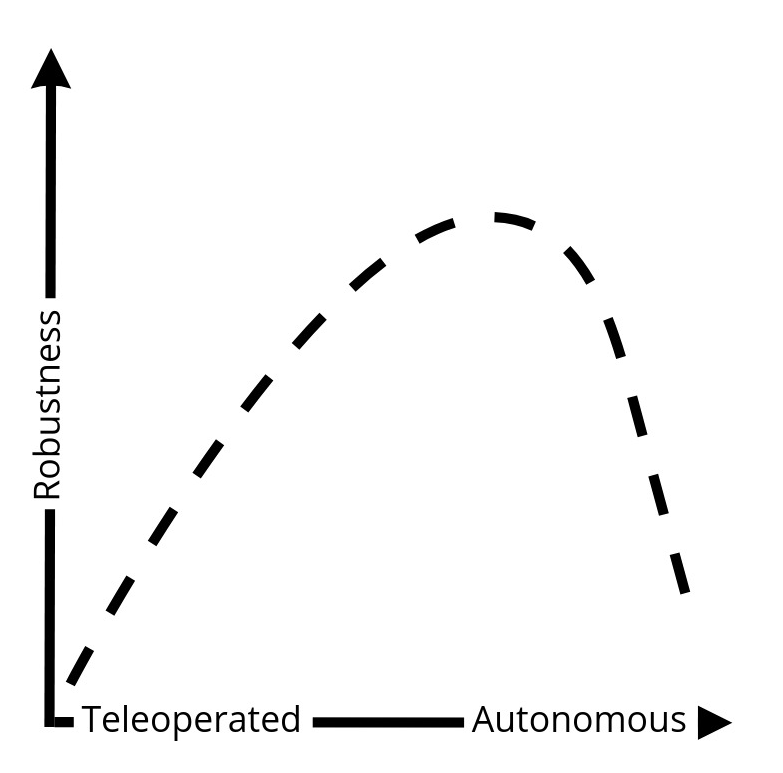
\includegraphics[width=0.45\textwidth]{pics/autonomy_robustness.png}
    \caption{\textsc{TODO: Maximum robustness is achieved through a compromise}}
    \label{fig:autonomy_robustness}
\end{figure}
\noindent
It is obvious, but also important, that in a dynamic environment it is not possible to anticipate every possible type of failure and respond with appropriate recovery.
\cite{Meeussen:2011} For Meeussen et al., this is another motivation for including a human operator as a fallback solution. Their key insight for this thesis is the importance of having
a human \textquote{in-the-loop} to achieve robust long-term autonomy, where the robot acts autonomously most of the time but has the option to request help from a human operator
when needed. They strongly suggest that this type of semi-supervised control, with a focus on fault detection and recovery, has the potential to realize systems that actually deliver
practical benefits.\newline
Dayoub et al. \cite{Dayoub:2011} intend to equip long-term autonomous mobile robots with the ability to localize in changing environments. It is an early work on long-term mapping,
i.e. updating environmental knowledge over time, which, unlike static representations, takes into account the inherent dynamics of the real world. The authors facilitate the concepts
of long-term and short-term memory as well as hybrid metric-topological maps.\newline
In \cite{Veloso:2012}, Veloso et al. present their autonomous mobile service robots for indoor applications, which they call \textit{CoBots} (2012). Of particular interest to this thesis
is their focus on symbiotic autonomy, through which the authors allow the \textit{CoBots} to overcome their specific limitations by requesting help from humans.
Additionally, they propose to investigate robust execution monitoring strategies.\newline
Tipaldi et al. \cite{Tipaldi:2013} introduce a probabilistic localization framework for long-term autonomous systems, particularly acknowledging environment changes during
long-term operations. They state that previous approaches to localization in dynamic environments often treated dynamic objects as outliers and that this is insufficient
for semi-static objects that are naturally part of such environments.\newline
It should be noted that there is not a great deal of research providing actual long-term experiments with autonomous robots, mainly for two reasons:
Long-term studies are obviously more time-consuming and tedious, especially in real-world outdoor environments, and furthermore it is only in recent years that it has become
reasonably realistic to conduct such experiments based on technological progress. \cite{Leite:2013}\newline
In a special issue on long-term autonomy (2013), Barfoot et al. \cite{Barfoot:2013} ask what challenges need to be solved to bring long-term autonomous robots into the real-world. They are concerned with
two main subjects: Localization and mapping in dynamic environments and lifelong learning. The general theme under which one could summarize this special issue is the idea that it is
not possible to know every relevant aspect of the world in advance - these robots must have learning capabilities.
In accordance with this, Mühlfellner et al. \cite{Muehlfellner:2015} present an approach for lifelong visual localization and mapping based on three steps:
\begin{enumerate}
    \item Offline map generation based on multiple recordings (incorporating environment dynamics)
    \item Selection of landmarks that are considered useful for localization
    \item Online localization
\end{enumerate}
The authors have an interesting facet to their approach: \textquote{\textit{[...] we are concerned not so much with maintaining an accurate model of the world, but rather with
maintaining a useful model.}} \cite{Muehlfellner:2015}\newline
In 2016, Biswas et al. \cite{Biswas:2016} discuss results and insights from deploying a team of mobile service robots (\textit{CoBots}) in dynamic, unstructured real-world office environments
for extended periods of time. They emphasize the need for execution monitoring, which they incorporate in the form of scripts that monitor the progress of tasks and relay help
requests to human operators as needed. A particular focus of the work is on the robustness of the systems and understanding the nature of faults through extensive logging.
Ultimately, they require the intervention of human operators only in very rare situations and provide stable, long-term autonomous operation in the office environments considered.
\newline
Of course, there are not only long-term autonomous ground vehicles (AGVs). There is perhaps even more literature regarding the application of autonomous underwater vehicles (AUVs)
(e.g. \cite{Jones:2012}, \cite{Spears:2014}, \cite{Kunz:2009}, \cite{Chrpa:2015}, \cite{Harris:2021}) and unmanned aerial vehicles (UAVs) (e.g. \cite{Brommer:2018}, \cite{Dong:2014},
\cite{Dong:2017}) for extended periods of time. AUVs are particularly used for scientific observations and security applications. \cite{Chrpa:2015}
Steinberg et al. \cite{Steinberg:2016} debate challenges and opportunities for long-term autonomous systems in
maritime applications. They argue that many of the previous attempts in the literature targeting autonomous systems fail when the environment varies during deployment, e.g.
due to weather or seasonal effects. The work identifies three main types of challenges for long-term autonomous systems:
\begin{enumerate}
    \item Transience of initial knowledge of state, environment, goals, etc.
    \item Insufficiencies of traditional fault monitoring / diagnosis due to extended operating times
    \item Demand for context-based constraints, priorities and goals
\end{enumerate}
The authors highlight that most autonomous maritime operations in the literature are of short duration and that humans must intervene whenever an unexpected situation arises. 
Furthermore, the work underlines the demand for robust solutions even when the environment and context changes heavily. What will also be of particular importance
in this thesis is their view of the human operator. They do not envision autonomous systems that should completely abandon human cooperation, but point to the importance of
appropriate communication channels (dialogue / explanations) for autonomous systems.\newline
One approach to long-term autonomous navigation is vision-based route following, which enables robotic systems to autonomously follow routes that were previously demonstrated
manually. \cite{Paton:2016} However, as the authors claim, to be able to use such approaches in actual long-term scenarios, the algorithms must be able to address the challenge
of extreme appearance changes in dynamic outdoor environments. The work presents a route following algorithm for autonomous systems that addresses the problem of changing appearance
by facilitating multiple channels of information, allowing to extend the autonomous capabilities to longer time periods. Yet, the paper claims that this approach is insufficient for
true long-term autonomy that covers seasonal changes and point to the promising field of multi-experience localization.\newline
Palomeras et al. \cite{Palomeras:2016} are investigating robust long-term autonomous underwater vehicles in real-world environments with a focus on minimizing human surveillance.
The authors point out that this requires methods for error detection and correction. The work is mainly focused on developing a framework that integrates many aspects previously
demonstrated into a holistic and robust solution. They are able to demonstrate a reasonably functioning system, but also hint that future work will need to enhance robustness to
unexpected failures, e.g., by incorporating redundancy.\newline
One of the most influential projects in the field of long-term autonomous robotics is the \textit{STRANDS} \cite{Hawes:2017} project (2017). The goal of the project is to integrate all the
artificial intelligence and robotics technologies necessary to create a long-term autonomous mobile service robot in a care facility environment. Thus, it is again an example for a project
that focuses on indoor environments. Special emphasis is placed on the application of the systems in real everyday environments as opposed to specific laboratory installations.
Furthermore, the robots are supposed to improve their behavior during their long-term missions by learning the dynamics of their environment, thereby increasing their robustness.
For the authors, the attribute \textquote{long-term} implies that the robot should be able to run continuously and autonomously in its environment for at least several weeks, which requires
a certain resilience.
An example of a study that emerged from the \textit{STRANDS} project is a study of autonomous service robots deployed in a nursing home by Hanheide et al. \cite{Hanheide:2017}.
Although the work concentrates on aspects of human-robot interaction, it is a relevant example of long-term autonomous use of a mobile robot in a real-world environment.
Their robot was in fully autonomous operation for $63$ days.\newline
Santos et al. \cite{Santos:2017} focus on spatio-temporal environment representations during long-term autonomous operations of mobile robots with the goal of constantly updating
and refining the robot's knowledge of its dynamic environment during the application. They view it as a never-ending task of acknowledging environmental changes, which is a key
requirement for long-term autonomy without human intervention. \cite{Santos:2017}
Another method for long-term spatio-temporal mapping in a mobile robot scenario in dynamic environments is presented by Krajnik et al. \cite{Krajnik:2017}. Their work is also
based on the assumption that environmental changes are usually subject to certain periodicities and routines. They are able to represent dynamics and predict future conditions
in the robot's environment.\newline
Schuster et al. \cite{Schuster:2017} introduce the \textit{Lightweight Rover Unit (LRU)} and study autonomous planetary exploration with its specific hurdles, such as
inherent communication delays. Due to these delays, teleoperation is generally infeasible for planetary rover applications, and a certain level of autonomy is mandatory for successful
operation. \cite{Schuster:2017} Leaving aside all the aspects that are crucial for missions on other celestial bodies but less relevant to the scenario of this thesis, there are
still a number of useful insights. For instance, their view of robustness based on local recovery. Whenever a malfunction occurs due to certain environmental conditions, this should
be recognized and dealt with locally. \cite{Schuster:2017} The authors propose defining fallback strategies for such cases, such as retrying the procedure in the simplest case. Even
under the severely limited communications with planetary rovers, the authors emphasize the need for external (ground station) monitoring and intervention capabilities, which they
consider obligatory for any system operating in an unknown environment. Thus, they rely on shared-autonomy whenever necessary. The work describes various recovery methods for failure
cases, such as scripts that can be used to reinitialize failed hardware components or to adjust parameters. Another crucial aspect for increasing robustness is seen by the authors
in redundancy, which seems reasonable in light of the limited response options due to the communication delay.\newline
Del Duchetto et al. \cite{DelDuchetto:2018} address navigation failures in long-term autonomous mobile robot applications with a human-in-the-loop learning approach that provides
recovery policies. The approach is based on the \textit{learning by demonstration} paradigm that facilitates human demonstrations to learn failure situations and appropriate recoveries.
Whenever a robot is confronted with a situation for which it has no recovery strategy, it requests a new demonstration. As many before, the work deals with long-term service robots to be used
in indoor environments populated by humans, specifically in nursing homes. The authors fundamentally share the global goal of this thesis and focus on one specific aspect, namely the
detection and correction of navigation failures, but they also emphasize the need for a general framework for error detection and resolution for long-term autonomy.\newline
Han et al. \cite{Han:2018} work on a sub-field of long-term autonomy that has received a lot of attention in recent years - long-term place recognition. This is an important aspect
of long-term autonomous systems, particularly in outdoor scenarios. Outdoor environments over extended periods of time are naturally subject to significant change (day time,
seasons, etc.). \cite{Han:2018} Their method for long-term autonomous place recognition \textit{HALGE (Holism-And-Landmark Graph Embedding)} represents places by using both semantic
landmarks and holistic scene information. The idea of long-term location recognition is to be able to detect whether the place where a robot is currently located is a
previously visited place and, if necessary, to identify it in the history (loop closure). \cite{Han:2018} Long-term place recognition is an essential milestone on the way to robust
localization and thus long-term autonomy of mobile robots in general.\newline
In 2018, Brommer et al. \cite{Brommer:2018} study long-term autonomy of unmanned aerial vehicles, which are also commonly used for monitoring purposes in precision agriculture. One problem with using such
systems in long-term scenarios is their limited battery capacity, which allows only relatively short deployments, e.g., of $15$ minutes. \cite{Brommer:2018}
To address this drawback, the authors develop an autonomous landing and recharging procedure. Since GPS is not necessarily accurate enough, the authors use a visual approach to
landing. They also introduce a state monitoring system that keeps track of critical aspects such as unexpected low battery and triggers a response when needed.\newline
A further very relevant work is written by Kunze et al. \cite{KunzeSI:2018}, who discuss challenges for long-term autonomous robots in real-world environments and how these can be addressed with techniques from the field of AI.
First, they note that such systems must be both hardware and software robust, meaning that the systems must be able to cope with any potential environmental changes expected
during their deployments. \cite{KunzeSI:2018} They point out that much of the long-term autonomy research focuses on coping with changing environments. The work suggests that
long-term operation could be an opportunity to improve the robustness and overall performance of the robot over time, e.g., through log analysis and manual improvements or machine
learning approaches. The key message of the special issue is that there are numerous applications and opportunities for using AI methods to achieve or improve long-term autonomy,
or in other words, for combined research of AI and long-term autonomy.\newline
A recent example of long-term autonomous tour guide robots is provided by Wang et al. \cite{Wang:2018}. They state that autonomous robots deployed over a long period of time are
particularly prone to failure, as the duration of the deployment introduces more uncertainties and corner cases that rarely occur in short-term applications. Based on their deployed
robots \textit{TritonBot} and \textit{BoxBot}, they are able to closely investigate problems in terms of long-term autonomy and resilience. In particular, they draw attention to
certain hardware and software failures, infeasible workflows, and human-robot interaction problems. The authors underline that certain errors are inevitable and that it is therefore
crucial to equip the robot with failure detection and fail-safe capabilities to achieve a certain level of reliability. Furthermore, they claim that it may be useful to establish a form
of component-level monitoring, which is fairly consistent with the approaches described in section \ref{sec:sim_and_mon_of_lta_challenges}. Another important aspect the authors
stress is that certain failures, especially hardware failures, occur so infrequently that they often go unnoticed. However, since they will occur in long-term autonomous operation,
it is essential to find a way to systematically and reproducibly evaluate potential failure cases, e.g., through simulations. \cite{Wang:2018} This is precisely the rationale behind
all the simulations described in section \ref{sec:sim_and_mon_of_lta_challenges}. The paper also suggests that it is advisable to design the software components in such a way that
they tolerate the temporary unavailability of other components and wait until the recovery is completed. Finally, as a further important remark for this thesis, they note that
comprehensive logging in long-term autonomous applications offers great potential for evaluation, testing, and learning, e.g. through the use of the ROS tool \code{rosbag}.\newline
Egerstedt et al. \cite{Egerstedt:2018} consider a long-term autonomous environment monitoring scenario in which they define survival constraints inspired by the bond between
biological organisms and their environment in ecology. First, the authors highlight the unique challenges of long-term deployment in a dynamic, unstructured environment, such as
agriculture, noting that robots must have adaptive capabilities and manage problems potentially affecting their survivability. \textquote{\textit{The basic issue of survivability
over long time periods remains an open problem for autonomous robotic systems in uncontrolled environments.}} \cite{Egerstedt:2018} The work claims that survivability has been
previously addressed either by planned tasks that enforce survivability, such as battery station revisits in the scenario described in section \ref{sec:lta_plant_observation},
or by defining specific survivability goals that are combined with other objectives, i.e. multi-objective optimization. However, the authors point out that survivability is a
necessary condition for any successful operation and therefore a constraint-based approach may be preferable, based on the idea of ensuring survivability during the optimization
of an objective function. A very important aspect of long-term autonomous applications highlighted in the paper is that \textquote{\textit{[...] any assumption about environmental
stationarity, or even predictability, are doomed to be incorrect}}. \cite{Egerstedt:2018} They conclude that drastic environmental changes can lead to infeasible assumptions and
dysfunctional controls. Thus, they prefer to rely on low-level constraints that ensure safety and robustness and assume nothing about the environment.\newline
An important overview of the state of the art in artificial intelligence for long-term autonomy has been provided by Kunze et al. \cite{Kunze:2018}. The authors point out that there
are still many challenges to be overcome with respect to the reliable deployment of long-term autonomous robots in dynamic, partially unknown real-world environments. As essential
AI building blocks, they identify \textit{navigation \& mapping}, \textit{perception}, \textit{knowledge representation \& reasoning}, \textit{planning}, \textit{interaction}, and
\textit{learning}. All of these aspects have been major research areas in the AI / robotics literature for decades. The survey emphasizes the importance of bringing all of these
facets together to actually create systems that work in a practical way. Particularly relevant to this work are the identified natural challenge of system integration, i.e.
integrating numerous methods and technologies into a comprehensive solution for long-term autonomy, as well as the design of ``human-in-the-loop'' systems capable of utilizing the
help of human operators in unexpected problematic situations. \cite{Kunze:2018}\newline
A very recent example of a long-term autonomous mobile robot serving as a tour guide in a museum is provided by Del Duchetto et al. \cite{Duchetto:2019}, who present their robot
\textit{Lindsey} (2019), which is designed to have better social abilities compared to previous models. However, since the focus of this thesis is not on human-robot interaction, another aspect of the work is of
greater relevance - their approaches to dealing with contingencies. A useful monitoring interface that can be used to observe and, to a limited extent, control the robot via a web
application is developed. They note that it is obligatory for long-term autonomous robots that operate without the supervision of a human operator to be able to communicate
problems and situations that the robot cannot handle itself. In the work, a ROS module is developed in which operators can specify problematic conditions that are then constantly
checked during runtime. As soon as such a condition occurs, the information is transmitted via a specific channel. This allows the operator to respond to faults without having to
permanently monitor the robot's activities. Human-robot communication in this thesis operates in an analogous manner (cf. section \ref{sec:fallback_solution}).\newline
Tomy et al. \cite{Tomy:2019} study a specific aspect of long-term autonomous mobile robots, namely their charge scheduling. It is emphasized that the actual operating times of
such systems are mainly determined by their battery capacities and that most systems simply use certain thresholds to determine charging stops. With the work, the authors attempt
to improve this by relying on the fact that long-term autonomous robots have ample opportunity to learn adequate charging times and match them to natural idle times, etc.\newline
Krajnik et al. \cite{Krajnik:2019} and Fentanes et al. \cite{Fentanes:2015} propose methods for modeling and dealing with variations in the environment in long-term mobile robotic
applications caused by human activities or natural processes, based on the assumption that such events are often periodic and not entirely random. They claim that the long-term
nature of such operations is not only a challenge but also a chance to learn how the environment changes and to identify certain regularities. They further note that this ability
allows the robot to predict the future state of the world based on the recognized patterns, which certainly has a positive impact on long-term autonomy performance.\newline
With manipulation under uncertainity, Lanighan et al. \cite{Lanighan:2019} work on another aspect of long-term autonomous robotics. They consider a robotic system with a monitoring and
cleaning task in a dynamic environment where it is expected to operate autonomously for extended periods of time without human supervision. They see the uncertainty in unstructured
dynamic environments as the greatest challenge to long-term autonomy and highlight the need for planning and execution approaches capable of dealilng with such uncertainties and
inherent risks. They model the problem as a \textit{Partially Observable Markov Decision Process (POMDP)}, plan in the belief space, and try to avoid unrecoverable situations by
managing the stochastic actions.\newline
Recently (2020), Basich et al. \cite{Basich:2020} introduced a method for robots to improve their competence during long-term autonomous applications. Their particular focus is on so-called
\textit{competence-aware systems}, which are able to rate their own feasible level of autonomy under certain circumstances. This competence must be learned through feedback
(reinforcement learning) from human operators. The idea is that over time, the level of autonomy increases and the dependence on the human operator diminishes as the robot creates
finer models of its environment.\newline
Also just recently, Kyberd et al. \cite{Kyberd:2021} presented their work on long-term autonomy in diverse outdoor environments. They emphasize that the focus in the literature to date
has been on indoor environments due to hazardous weather conditions and the like in outdoor settings. The work introduces design principles for unmanned ground vehicles suited to the specific
intricacies of operating outdoors, with special emphasis on redundant safety layers and the ability to function in harsh weather and lighting conditions. Since their systems
lacks an autonomous charging procedure, a human operator is notified whenever the robot needs to be recharged. The authors indicate that in the future they will aim for autonomous
charging, e.g. by inductive charging, so that the entire operating cycle can be captured autonomously. This is exactly what the integration of autonomous docking described in section
\ref{sec:docking_solution} aims to achieve in this work.\newline
Eventually, in 2021, Emam et al. \cite{Emam:2021} present a \textit{Control Barrier Function (CBF)} framework to tackle the problem of perturbations that the robot may face. The authors
underscore that when developing new algorithms for robots operating autonomously for extended periods of time in dynamic environments, it is imperative to pay close attention to
robustness in order to deal with all the challenges potentially occuring in such situations (cf. section \ref{sec:challenges_for_lta}). As they claim:
\textquote{\textit{[...] if these disturbances are not addressed, the possibility of failure becomes almost assured if the robots are required to operate over long time horizons.}}
\cite{Emam:2021} Accordingly, the work indicates the need for robust control mechanisms capable of dealing with such contingencies.\newline

\noindent
\textit{Execution Monitoring.}\newline

\noindent
An early work on execution monitoring in robotics is by Pettersson \cite{Pettersson:2005}. The author attempts to transfer the knowledge of \textit{fault detection and isolation
} (FDI) commonly used in industrial control to the field of robotics. The work already highlights the requirement for execution monitoring when planning the deployment of robots in
dynamic environments, e.g. due to lack of information, unreliable resources, or stochastic effects. Pettersson discusses several attempts to deal with uncertainty, but notes that
there is no way to completely eliminate uncertainty in partially observable dynamic environments and that systems must tolerate some degree of uncertainty. The paper asserts that
systems must expect faulty execution from time to time, e.g. by including execution monitoring as part of the control architecture. This is exactly what is done in this thesis
(cf. \ref{sec:execution_monitoring_smach_architecture}). Pettersson compares several definitions for execution monitoring. A classic variation from the field of AI is the
identification and classification of inconsistencies between observations and predictions, and mechanisms to recover from these inconsistencies. \cite{Pettersson:2005}
However, according to this definition, only systems with predictive models can perform monitoring. \cite{Pettersson:2005} A second definition, which comes more from an
industrial control perspective, defines it as a continuous process of real-time information acquisition that determines the state of the system and signals anomalies.
\cite{Pettersson:2005} Based on the literature, Pettersson proposes three types of general functions of a monitoring procedure, the first two of which are more or less mandatory:
\begin{enumerate}
    \item fault detection \textrightarrow $\thinspace$ recognizing problem
    \item fault isolation \textrightarrow $\thinspace$ classifying error type
    \item fault identification \textrightarrow $\thinspace$ rating severity
\end{enumerate}
Based on the definitions in the paper, the execution monitoring procedures described in section \ref{sec:sim_and_mon_of_lta_challenges} fall under the category of data-driven
approaches, where fault detection and isolation are based on the (statistical) evaluation of the input data. Statistical analysis assumes that data variability changes drastically
only in problematic situations and is otherwise relatively stable. \cite{Pettersson:2005} Many of the monitoring methods presented in this thesis involve comparing an input signal
to a specified limit (cf. \ref{sec:sim_and_mon_of_lta_challenges}), which is called \textit{limit value checking} and is very common in industrial control. \cite{Pettersson:2005} However, the methods in this thesis are also
quite well aligned with the core ideas of expert systems (knowledge-based systems), which often represent knowledge with conditional statements. \cite{Pettersson:2005} Pettersson,
like many other authors, points out that one of the most common problems in the field of mobile robotics is that methods and solutions are developed and tailored for a specific
system and the generalizability is rather limited, which is a motivation for developing solutions that are as general as possible but still useful.\newline
Vechet et al. \cite{Vechet:2015} state that fault detection is underexposed in robotics research and development, but is nonetheless fundamental to the
deployment of autonomous mobile robots. They see a demand for health monitoring to prevent system failures and present a Markov chain model for \textit{Failure Detection and
Identification (FDI)}.\newline
Iocchi et al. \cite{Iocchi:2016} develop a framework for plan generation and execution with a focus on robustness by addressing certain shortcomings of classical plan execution
monitoring approaches. They are evaluating the framework in a service robot application in public, human-populated environments such as shopping malls and offices. A critical
challenge in such an environment, identified in the paper, arises from the fact that the robot must interact with inexperienced users. In particular, they highlight the great
significance and need for planning under uncertainty, execution monitoring solutions, and the combined consideration of planning and execution when it comes to the use of
autonomous robots in real-world environments populated by humans. The framework proposed in the work relies on \textit{Progressive Reasoning Units} and \textit{Petri Net Plans}
and is, like many works in the literature considering monitoring, particularly focused on plan execution.\newline
Winder \cite{Winder:2016} proposes an anomaly reasoning framework capable of recognizing and responding to previously unknown entities and situations, with the overall goal of
increasing an agent's versatility and robustness in dynamic environments. The author postulates the hypothesis that such an approach requires the integration of machine learning
methods and systematic knowledge representation.\newline
Khalastchi et al. consider \textit{fault detection and diagnosis} (FDD) for robotic systems, which is necessary for recovery from problematic situations and thus
robust long-term operation. \cite{Khalastchi:2018} The application of FDD to robotics is a relatively new field of research, but one that is very crucial
because errors can disrupt a robot's mission, reduce its efficiency, or even pose safety problems for itself or the environment. \cite{Khalastchi:2018} The paper notes that it is
critical that the detection of a problem is followed by some form of diagnosis that identifies the affected component and supports the recovery process. The authors provide a useful
fault taxonomy for robotic systems in which they generally divide hardware (detection, action), software (algorithms, implementations), and interaction (internal / external) faults.
Knowledge-based FDD methods, e.g. expert systems such as the ones proposed in section \ref{sec:sim_and_mon_of_lta_challenges}, are essentially based on predefined issues and
diagnoses. \cite{Khalastchi:2018} The authors note that internal sensors that provide information about the current state of the robot can be facilitated in FDD. In addition,
exteroceptive sensors should be used for this purpose, but of course they can be used not only for FDD, but also can be the target of FDD in case of sensor failures. \cite{Khalastchi:2018}
As a major challenge, the authors see the real-time nature of robotic applications, where erroneous situations must be detected as quickly as possible so that the robot can resume
its operation. Usually, FDD must be performed on board the mobile robot, which imposes significant constraints on computational resources. \cite{Khalastchi:2018} As mentioned earlier,
the monitoring approaches in this thesis are model-free, which has the advantage of providing some generality and thus transferability to other systems and scenarios. \cite{Khalastchi:2018} 
In addition, the authors emphasize that trying to model every aspect of the system as well as its interaction with the environment is very complex and often infeasible.
However, they also illustrate the disadvantage of expert system approaches, namely dealing with the unknown, since it is not trivial to extrapolate from a fixed ruleset.\newline
A somewhat different perspective is provided by Honig et al. \cite{Honig:2018}, who review methods for fault detection and recovery with a particular focus on human-robot interaction. Nevertheless, the work contains several aspects
that are quite relevant for this thesis, despite their different focus. First, like many authors before, they emphasize that robots working in dynamic real-world environments are
constantly confronted with errors and that there is still a lack of proper error management methods. Consistent with the literature, they define a \textit{failure} loosely as a
state in which the performance provided by the robot deviates from the norm, caused by one or more \textit{errors}, which they consider system conditions that lead to such
situations. Additionally, they consider \textit{errors} as the result of \textit{faults}, which are ultimately the reason why the system gets into such an error state.
[TODO: Apply this terminology to the thesis?] The authors discuss numerous taxonomies for classifying failures and compare various concepts from the literature. Of particular
interest to this work is the concept of terminal failures that break the current mission of the robot, non-terminal failures that merely affect the outcomes or performance and
reparability of such cases. Also useful is their discussion of failure categories, which largely coincide with the categories of Khalastchi et al. (interaction, hardware, software).
\cite{Khalastchi:2018}. The authors themselves focus on the distinction between technical failures (hardware + software) and interaction failures (environment + other actors).
Of crucial importance to this work is the authors' finding that the involvement of a human operator in certain critical situations is computationally cheaper than comparatively
costly and often unreliable other approaches. To do this in the most effective way, the problem should be communicated as precisely as possible. \cite{Honig:2018}\newline
Mauro et al. \cite{Mauro:2019} introduce a high-level deep learning and vision based approach to execution monitoring for robot tasks. Monitoring is again limited to the execution of the
plan and not to the operation of the robot in an environment in general. They evaluate their approach with a humanoid assistant robot in a warehouse environment and report some
promising results. However, as mentioned, it is only considering very specific tasks and high-level actions.\newline
Recently, Harris et al. \cite{Harris:2021} presented an execution monitoring and online plan modification approach that considers aspects such as resource availability
and goal reasoning. The approach is evaluated in a long-term AUV scenario with very limited opportunities for human intervention and a highly dynamic and uncertain environment.
Their method is based on the idea of altering the plan as needed, e.g. adding goals when resource consumption is lower than expected and removing goals (starting with those with
low priority) when it is higher than expected. In order not to generate infeasible plans, the method relies on information about the causal relationship between actions. In cases
where resources are uncertain, one approach is to provide branches in plans that allow a decision to be made between multiple options based on available resources. \cite{Harris:2021}
The general monitoring and resolution approaches developed in this thesis are not as tethered to a plan, but the overall ideas and goals are similar.\newline
Not necessarily focused on execution monitoring, but a good motivation for its necessity is provided by \cite{Roucek:2021}, which asserts that research papers are
usually concerned with aspects such as accuracy or computational complexity of their methods, but not so much with their reliability in integrated systems such as robots.
And further: \textquote{\textit{[...] the performance of robotic systems cannot be optimal in real-world situations which are impacted by the robustness of the deployed systems}}.
\cite{Roucek:2021} They conclude that the successful deployment of robots in real-world environments fundamentally depends on reliability and interoperability aspects of the
employd submodules, which is a great motivation for this thesis.\newline
Very recently, Coruhlu et al. \cite{Coruhlu:2021} studied plan execution monitoring for autonomous systems. They point out that it is critical to equip robots with the ability
to recognize and respond appropriately to deviations between expectations and observations, focusing particularly on diagnosis and explanation. Although at first glance their work
appears to be very closely related to this thesis, their focus is quite different in that they are concerned with high-level monitoring of plan execution, dealing in particular with
partial observability. As with most execution monitoring work in the literature, the focus is on plan execution rather than general robot operation in an environment, recovery often
relies on replanning.\newline

\noindent
\textit{Environment Monitoring and Agricultural Robotics.}\newline

\noindent
An early example of automated crop monitoring in its broadest sense is forest inventory. Lalonde et al. \cite{Lalonde:2006} address the task of automatic and accurate tree counting and
diameter estimation based on $3D$ point cloud processing. The motivation in this area is similar to the classic field scenarios: Optimizing efficiency and reducing manual labor.\newline
Singh et al. \cite{Singh:2010} present their results and findings from operating a reconfigurable autonomous driving system on a farm. Their overall goal is to integrate technologies
from the field of robotics with plant science to increase production efficiency. Based on the reconfigurable tool and sensor setup, they aim to use the systems to improve the
efficiency of various agricultural operations such as harvesting, spraying, plant inspection, tree counting, etc. The vehicle drives autonomously in the sense that it detects and
follows rows of trees in an orchard based on laser scans. One of the most important insights, which may also be relevant to this work, is that it is crucial to keep the project
consistent with the actual requirements of the intended users and real-world applications. Only then can the result actually be of use to practitioners.\newline
Xue et al. \cite{Xue:2010} present a vision-based system also capable of guiding a mobile robotic platform trhough crop rows in a field, thus enabling autonomous navigation
in a field. The work stresses the need for reconfigurable platforms that can, in principle, be used for various agricultural tasks, depending on the particular sensor equipment.
\newline
A comprehensive overview of robotic systems (AUVs, AGVs, UAVs) for environmental monitoring, e.g. deep-sea or volcano exploration, is provided by Dunbabin et al. \cite{Dunbabin:2012}.
The authors underscore the urgent need for long-term autonomous environmental monitoring systems to cope with natural catastrophes such as earthquakes, tsunamis, forest fires, volcanic
eruptions, etc. In a nutshell: \textquote{\textit{[...] scientists see robotics as a promising tool with the capacity to improve their current means to observe and collect
data about natural processes or phenomena at vast spatial and temporal scales.}} \cite{Dunbabin:2012} They view robots essentially as mobile sensors that are used to understand
the environment. Although there is an undeniable demand for such systems, the authors note that there is a lack of robustness, reliability, and security for a widespread use,
which could be addressed by fault-tolerant systems and redundant hardware components. \cite{Dunbabin:2012}\newline
Dong et al. \cite{Dong:2014} present an imaging method for crop monitoring based on both AGVs and UAVs. Traditionally, manual labor has been required to collect samples, which is
obviously not suitable for monitoring large areas over long periods of time. \cite{Dong:2014} Therefore, as the authors point out, imaging methods have been developed to enable
remote sensing and reduce the human effort required for data acquisition. Originally, hyper-spectral satellite imagery was used with the disadvantage of limited spatial and temporal
resolution. \cite{Dong:2014} Thus, they introduce a crop monitoring approach that uses UAVs or AGVs and methods from computer vision to increase the efficiency of crop imaging.
The goal of the work is to create a $4D$ representation of plant development based on high-resolution imagery and GPS / IMU data. The overall goal of the work is to increase the
efficiency of agricultural production by replacing time-consuming and costly human labor with highly efficient autonomous monitoring systems.
As an early work, however, it is still limited to manually operated vehicles and therefore disregards the aspect of autonomy.\newline
Bargoti et al. \cite{Bargoti:2015} introduce a system for automated tree detection on an apple orchard that combines image data and laser scans. The work highlights that information
acquisition and processing is becoming increasingly relevant for farmers trying to optimize the efficiency of their processes. The developed system is a UGV capable of autonomous
operation via intrarow nagivation. However, the authors point out issues regarding localization reliability and GPS connectivity that need to be addressed in future work.
This is a strong motivation for two of the challenges discussed in section \ref{sec:challenges_for_lta}.\newline
Carlone et al. \cite{Carlone:2015} highlight that recent advances in mobile robotics, particularly UGVs and UAVs, are increasingly providing a realistic alternative to
inefficient, labor-intensive manual work in the task of continuous crop monitoring. They target a specific aspect of crop monitoring and create $3D$ representations over time,
resulting in an overall $4D$ model of plant evolution. \newline
Virlet et al. \cite{Virlet:2016} choose a completely different approach of automating plant phenotyping. They are developing an automated field phenotyping platform, but instead of
relying on (autonomous) vehicles, they are building a sensor array mounted on stationary rails above the rows of plants to be monitored. They argue that such a system has the
advantage of completely eliminating the need for human supervision, which is not yet the case with vehicles. A further disadvantage of vehicle-based monitoring systems is their
impact on the soil structure and their potential damage, especially because of the continuous nature of the operations. \cite{Virlet:2016} Thus, they provide an interesting
alternative to autonomous monitoring using AGVs, which arguably has a higher initial effort to set up such a monitoring structure, but may be more reliable and soil-protecting,
at least with the current state of the art of AGVs. However, one could argue that such an approach may not scale for very large field areas.\newline 
Another semi-autonomous mobile ground vehicle for crop monitoring is presented by Bietresato et al. \cite{Bietresato:2016}.\newline
Bechar et al. \cite{Bechar:2016} provide an overview of the current state of the art of agricultural robots for field work. The authors particularly emphasize that the various
components that make up a robotic system must be integrated and synchronized to create a holistic system capable of performing in unstructured dynamic environments at least as
well and reliably as previously used methods, such as manual human labor. Successful systems that are rarely available on the market must be economically viable, safe and robust.
\cite{Bechar:2016} In specific, the authors stress the necessity of researching human-in-the-loop systems, as they see great potential in them for increased robustness and
reliability. The paper summarizes the extensive research that has demonstrated the potential of robots to address current and future problems in agriculture, particularly in terms
of production efficiency and environmental sustainability. As one of the biggest challenges in agricultural scenarios, they identify the unstructured and dynamic nature of the
environment, which changes over time and implies myriad unpredictable contingencies. Bechar et al. classify applications of robotic systems into four groups:
\begin{itemize}
    \item environment and objects structured
    \item environment unstructured and objects structured
    \item environment structured and objects unstructured
    \item environment and objects unstructured
\end{itemize}
They place the agricultural sector in the last and arguably most difficult category, which they see as a particular hurdle to commercialization. Based on their reasoning, it is
evident that the challenges to long-term autonomy that will be considered in this thesis are part of the barrier to commercialization. Another challenge identified in the work that
is particularly relevant to this thesis is that robotic systems and technologies developed for one specific agricultural use case are not necessarily reusable for others because they
are so different, i.e. it is difficult to find generic solutions. Nevertheless, it should be an important aspiration to develop solutions as generic as possible in terms of sensors
used, etc., which is taken to heart in this thesis. Regarding the autonomy of such systems, the authors believe that partially autonomous robots will undoubtedly be useful in
practice, even if they do not yet achieve full autonomy. The paper examines numerous research papers and concludes that there are very few commercially available solutions, all of
which are the result of iterative development for a very specific task. The authors note that the early examples of autonomous systems clearly suggest that the performance of the
system can be improved by human support in dynamically occurring problem situations, allowing some form of collaboration as human and robot capabilities tend to complement each
other. This is exactly the idea of this thesis, to cope with otherwise unsolvable situations. It is obvious that it is already a huge improvement when a robotic system can take over
a large part of the work and a human operator only needs to intervene once in a while in unpredictable and unsolvable situations. Full autonomy may be a reasonable goal to strive for
in the future, but it is not a requirement for improving productivity. The work also asserts that the most important aspect with respect to the numerous integrated components in a
robot is to provide methods capable of handling unexpected events, which is a great motivation for this work.\newline
In a later paper, Dong et al. \cite{Dong:2017} revisit autonomous crop monitoring with a focus on high temporal as well as spatial resolution. They claim that common $3D$ models do
not acknowledge the temporal aspect of crops that are continuously growing and changing. As in the previous work, they rely on UAVs and AGVs because of their potential to collect
data at high spatial and temporal resolution very efficiently. They present a crop monitoring method for $4D$ representation considering both space and time, as well as an algorithm
for robust data association that can deal with heavy environment variations. The work assumes a static environment during a data acquisition process, which means that it ignores
unexpected dynamic changes that can be expected in real-world environments and focuses on the evaluation of the proposed methods. Moreover, the aspect of autonomy is still not taken
into account.\newline
Ampatzidis et al. \cite{Ampatzidis:2017} provide an overview of robotics and AI methods and technologies applied to the field of plant pathology as well as precision agriculture
in general. In addition to the advancing automation of classic agricultural processes, there is an ever increasing focus on automated detection of plant deseases.
\cite{Ampatzidis:2017} According to the authors, it is crucial that further research and development of sophisticated autonomous robotic platforms for agricultural purposes
goes hand in hand with the development of diagnostic systems. Many of the incorporated AI methods, such as those from the field of computer vision, are developed independently of
the robotic systems that use them in practice. \cite{Ampatzidis:2017} Thus, the authors highlight the need for integrated testing and diagnosis.
Likewise, \cite{Roucek:2021} underlines the fact that robots consist of a large number of integrated hardware and software modules that are typically developed and
tested in isolation, which is why aspects such as system integration, interoperability, etc. often unjustly receive little attention.\newline
Roure et al. \cite{Roure:2018} study a monitoring and protection scenario in vineyards. Typically, human workers manually go through the field and distribute pheromone dispensers
to protect the plants. \cite{Roure:2018} The authors utilize a mobile AGV and focus on the necessary integration of state of the art robotics and AI techniques required to deploy
such a system.\newline
Very close to the scenario in this thesis in the work of Bayati et al. \cite{Bayati:2018}, which considers a mobile robot for crop monitoring. The authors present a high-throughput
plant phenotyping system for canola plants. Only such automated phenotyping systems are capable of efficiently providing the necessary information for plant breeding and related
genetic research. \cite{Bayati:2018} The authors claim that in 2018, there were no commercially available high-throughput plant phenotyping platforms (HTPPs) and especially no
autonomous vehicles. The goal of phenotyping is to identify desirable genetic responses to environmental stimuli in order to improve crop quality. \cite{Bayati:2018}
In the paper, a prototype of an automated HTP based on an agricultural vehicle is presented. However, it is not yet about full autonomy and especially not about long-term autonomy.
\newline
A recent work on real-time detection of crops for autonomous harvesting is provided by Montes et al. \cite{Montes:2020}. The work focuses on real-time detection of broccoli crops
in $3D$ point clouds.\newline
Very recently, Fountas et al. \cite{Fountas:2020} gave an overview of the state of the art in robotic systems for agriculture, especially for field work. The authors distinguish
the challenges that such robots might face in general and task-specific issues. The universal issues are more related to challenges that all AGVs might face in dynamic outdoor
environments (terrain assessment, route planning, safety etc.). \cite{Fountas:2020} Whereas task-specific issues are more related to the specific agricultural task. The authors
focus on problems specific to crop production, such as weed control, seeding, disease and insect detection, monitoring, phenotyping, spraying, and harvesting. Particularly relevant
to this thesis is the section on plant monitoring, where the authors underline the potential of automation in this area. There are systematic assessment tools such as
\textit{Ratio Vegetation Index (RVI)} and \textit{Normalized Difference Vegetation Index (NDVI)} that inform about important aspects of the overall plant health. \cite{Fountas:2020}
In general, the authors point out that robotics in agriculture has the potential to solve some of the fundamental efficiency problems that currently exist in the field. In summary,
they describe current research and commercialization efforts, highlight the technologies required for such systems, and hint to some potentials, particularly related to challenges
in computer vision that are ubiquitous in agricultural application of robots.\newline
Polvara et al. \cite{Polvara:2021} consider a specific issue related to the increasing use of autonomous mobile robots in agricultural environments where they collaborate with
human workers. The authors present a method for identifying and tracking human workers in such environments to enable robots to become useful assistants.\newline
Finally, Khak Pour et al. \cite{KhakPour:2021} present an implementation of an autonomous, mobile, ground-based HTPP for crop monitoring. However, autonomy refers to the
monitoring task, but not to the entire operation, as the tractor is a semi-autonomous vehicle. Nevertheless, since the authors consider their system ready for the commercial
market in principle, it is a good example for the fact that full-autonomy is not necessarily the paradigm to strive for, at least not to be useful.\newline

\noindent
\textit{Concluding Remarks.}\newline

\noindent
A substantial majority of the research described concerning long-term autonomy deals with indoor service scenarios. One could argue that this is a manual sample that may be biased,
however, it should fairly accurately reflect the focus in the literature. The examples available for outdoor scenarios tend to focus on very specific aspects of long-term autonomy,
such as environmental change and place recognition, which is briefly discussed in section \ref{sec:challenges_for_lta}. In addition, general problem handling capabilities are often
tightly tethered to specific systems and environments and therefore hardly reusable; sometimes they are not even explicitly described. What is perhaps a bit underexposed in the
literature is the big picture of long-term autonomous mobile robotic applications in outdoor scenarios, not focusing on specific aspects but approaching an integrated functioning
system. More precisely, work that discusses the common problems in all autonomous long-term scenarios, regardless of the specific application, and how to address them by merging
ideas from long-term autonomy and general execution monitoring. This thesis is intended as a step in the direction of thinking about a generic framework that is nevertheless specific
enough to be concretely applicable in the scenario under consideration. Referring to the overview of agricultural robotics, it should be emphasized that a fully autonomous mobile
robot is considered in this work. Most of the work in the literature considers autonomy in the sense that a system is able to autonomously follow plant rows, e.g., intrarow
navigation, but typically not a system that can freely and autonomously navigate through its environment. The work rarely considers full autonomy, and particularly not long-term
autonomy. As mentioned before, full autonomy is not necessarily the paradigm to strive for if the goal is to increase efficiency. Nonetheless, it is worth investigating full autonomy
for agricultural applications, whether or not it proves to be the best suited concept.

\section{Long-Term Autonomous Plant Observation}
\label{sec:lta_plant_observation}

The particular scenario that is going to be considered in this work takes place in an agricultural context. Therefore, the robot will be faced with a highly dynamic unstructured
environment. Long-term autonomy in known static environments is essentially solvable by a robust system that is able to
stay functional for extended periods of time. \cite{Kunze:2018} Such environments are often given in an industrial context where the robot must perform well-defined, repetitive tasks
in a stable and predictable setting. \cite{Bechar:2016}
In contrast, a highly dynamic, partially unknown environment such as in this scenario poses much more difficult
challenges, e.g., due to unexpected environmental changes that are hard, if not impossible, to anticipate.
Such environments are often referred to in the literature as \textquote{automation-averse}.
The idea is to enable a mobile robot to autonomously conduct 3D-Lidar scans and hyperspectral images of the plants on a field in order to monitor their growth progression and 
to detect certain features based on the growth stage. Moreover, these recordings can be used to detect leaf diseases [TODO: refine based on literature]. It is essentially a task of
data acquisition.
Correspondingly, the robot has to be able to process the entire field continually without the need for human supervision,
including the requirement for repeated charge stops. For this purpose, there is supporting infrastructure in the form of a container with an inductive charging station on site
establishing the power supply. Since the focus of the work is not going to be the scanning task, but to establish robust long-term autonomy, the actual detection of features 
etc. will be disregarded.
A crucial question is how to actually define ``long-term''. As Hawes et al. remark, it has no strict definition and can have various meanings depending
on the context, e.g. NASA's rover \textit{Opportunity} has been exploring the surface of Mars autonomously for years and autonomous wave gliders are able to monitor
ocean sections for months. Furthermore, there are mobile service robots used for extended periods of time in everyday, indoor environments like hospitals 
as examined in the STRANDS project. \cite{Hawes:2017}
For this work, in contrast, ``long-term'' is going to be defined in terms of the robot's temporal radius of action that is mainly based on its battery capacity, i.e. charge cycle,
but may also include aspects like maintenance intervals etc. In general, all processes that require a number of such cycles are considered long-term processes.
Accordingly, ``long-term'' can only be defined depending on the system in question. To give an example: There are systems with very limited battery capacity, 
such as toy drones. Based on absolute time, a two-hour experiment might not be regarded as being long-term, but if it involves multiple charging cycles, it can be 
algorithmically considered a long-term process. Consequently, ``long-term'' is relative.\newline
In the agricultural sector, there are processes that last much longer than a charge cycle, e.g. vegetation periods.
However, the seasonal cycle is not the sort of long-term process that will be investigated in this work, as such processes already exist on a much smaller scale.
On the one hand, there is the mission level, i.e. one processing of an entire field. 
Such a mission can already be regarded as long-term, since based on the dimensions of the particular field under consideration, it is not guaranteed that one
battery charge will be sufficient to process the entire field. Instead, one battery cycle will be defined as sufficient to process a certain fraction of the scan
positions, and a planner should maximize the number of planned scan stops in a mission under the constraint that a battery safety buffer is not undercut.
Thus, a key aspect of the scenario is going to be that the mission must be paused, the state must be saved, and the mission must be continued after recharging.
In the meantime, the environment may have changed, e.g. weather conditions or illumination, which is relevant for certain sensors of the robot.
On the other hand, there are going to be several such field processings during one vegetation period, which makes it a long-term process of repeated missions.
Hence, it takes a number of charge cycles to process the entire field, and that mission is going to be repeated every few days,
which means that there are two different long-term cycles that are intertwined.
These two cycles basically represent a lower bound for the length of long-term autonomous episodes in the scenario under
consideration. Likewise, in contrast to the above examples of Mars rovers and autonomous wave gliders, which are long-term
processes of arbitrary length, it is useful to think about natural upper bounds on the length of such episodes in agricultural
applications. Such a natural upper bound could be a time after which a human operator will inspect the robot anyway,
which in agriculture is certainly the case sooner than after a few months, e.g. during maintenance sessions 
when sensors such as cameras and laser scanners are cleaned, tire pressures are checked, etc.
After such a maintenance session, the new episode begins. 
Based on these bounds, it makes sense that the robot does not send every minor problem it recognizes directly to the operator,
but keeps a list of minor issues that do not require immediate action, but should be resolved during the next maintenance
appointment.\newline
Now that it has been sufficiently clarified how \textit{long-term} and \textit{mobile} are to be understood in the context of this work,
a precise definition of what is meant by the remaining attribute \textit{autonomous} follows.
Like the concept \textit{long-term}, \textit{autonomous} is not sharply defined in the literature and can have different meaningful connotations depending
on the context. Autonomy in the context of application-oriented robots usually has the goal of achieving a higher degree of automation in these applications,
i.e. using technical means so that a process runs completely or partially without involvement and supervision of a human operator. \cite{Hertzberg:2015}
Completely or partially already indicates that autonomy is not a binary attribute, but refers to a spectrum of different degrees of autonomy,
ranging from teleoperation at the lower end over shared and traded control up to full autonomy at the upper end. \cite{Hertzberg:2015}
Figure \ref{fig:autonomy_spectrum} summarizes these concepts based on \cite{Hertzberg:2015}.
\begin{figure}[H]
    \centering
    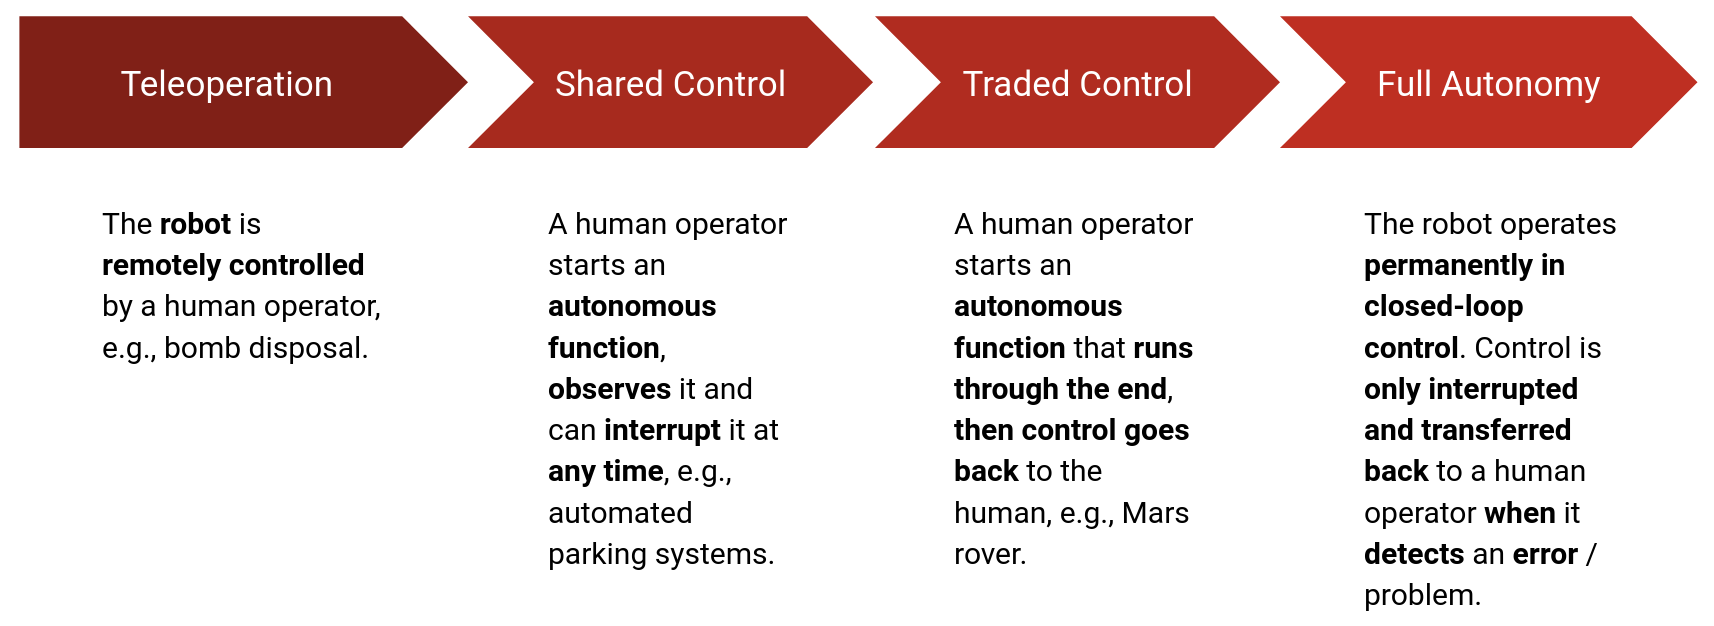
\includegraphics[width=\textwidth]{pics/autonomy_spectrum.png}
    \caption{\textsc{Autonomy Spectrum}}
    \label{fig:autonomy_spectrum}
\end{figure}
\noindent
Accordingly, autonomy does not necessarily mean that there is no connection to a human operator at all.
The concept of traded control is particularly relevant for robotics in space applications, e.g. satellites or planetary rovers.
NASA's Mars exploration rovers \textit{Spirit} and \textit{Opportunity}, for example, do not operate fully autonomously, but rely on human assistance for many tasks,
such as plan generation and evaluation. \cite{Bresina:2005} NASA calls the concept \textit{mixed-initiative planning}. Involving humans in control has the advantage of gaining
flexibility, which allows to dynamically react to unexpected situations. \cite{Bresina:2005}
The idea is that the robotic system operates autonomously in principle, performing all the repetitive routine tasks, but the human operator can take over in certain situations,
such as when the robot is in danger and human intervention is required, or when a task needs to be performed that for some reason is better suited for a human operator.
\cite{Kortenkamp:2009} There is even evidence that \textit{human initiative} systems that can switch between different autonomy levels during operation perform better than
systems with fixed autonomy levels, at least in certain environments. \cite{Chiou:2021}
The plant monitoring robot considered in this work, however, can be classified as fully autonomous in the sense of figure \ref{fig:autonomy_spectrum}, 
i.e. during a long-term autonomy cycle as defined above, the robot should only come into contact with a human operator when it detects an error or a problematic situation
that prevents it from continuing its task.

\section{Prototype Scenario in the Simulation}
\label{sec:prototype_scenario}

As starting point serves a physics simulation in \textit{Gazebo}\footnote{Open-source 3D robotics simulator} that has been created within the research project PORTAL \cite{portal}
and is adapted and extended as part of this work. The simulation includes the AROX model, i.e. a simulated version of the system described in section \ref{sec:robotic_system},
as well as a 2.5D reflection of a test field environment. For the prototypical baseline scenario of this work, the layout of abstract crops as objects of interest shown in 
figure \ref{fig:prototypical_layout} was created. Initially, the simulation works under the assumption that the robot is able to charge its battery as soon as it is located at 
certain coordinates as a simplification of the container infrastructure. These coordinates are visualized by the charge patch displayed in figure \ref{fig:prototypical_layout}.
In order to determine the robot's route through the field as well as the whole scanning processes, a plan is needed, i.e. when to drive to and process which parcel of the field. 
An example of a simple scan route can be seen in figure \ref{fig:example_scan_route}. Since this work does not deal with planning algorithms, it is simply assumed that the plans
are created by human operators. Hence, a plan is going to be a CSV file of actions. Plan generation and format are described in detail in section \ref{sec:plan_generation}, 
but in general plans will focus on two types of actions. The first type is \code{drive_to(lat, lng, theta)}, which causes the robot to drive to the specified latitude, 
longitude, and orientation (if possible), an action the employed robotic system AROX is capable of. The second type of action is \code{scan}, which initiates a scanning procedure
at the robot's current position. In practice, the real robot is equipped with a high-resolution 3D-Lidar sensor (cf. RIEGL sensor in fig. \ref{fig:arox_system}) that is going 
to be used to scan the field parcels with the aim of detecting features of the plants. To simulate the scanning procedure, some kind of dummy node is required that allows to 
scan on command (cf. section \ref{sec:dummy_scanning_node}), i.e. to simulate scanning, since we are not actually interested in any real scanning data. Thus, the second type 
of action will initiate a scanning procedure of the 3D-Lidar sensor or an execution of a dummy node, respectively. There are other actions, but these two are the very specific ones
relevant to the scenario under consideration; the details are described in section \ref{sec:plan_generation}. This prototypical scenario is the implementation of a minimal 
example of a long-term autonomous plant monitoring scenario in a simulation. Basic autonomous long-term functionality is provided, which means that the robot is able to 
complete its plant observation missions interrupted by several necessary charge stops. It will be used later to evaluate the challenges identified in section 
\ref{sec:challenges_for_lta} as well as the monitoring approaches presented in section \ref{sec:sim_and_mon_of_lta_challenges}.
The overall process implemented for each of the challenges considered is to simulate the occurrence of the respective issue, detect it using
the monitoring approaches developed in this work, interrupt the robot's normal operation, solve the problem, and transition back to normal operation to resume 
plan execution exactly where it was preempted. In terms of mapping, it should be noted that the global map of the environment for this scenario was created manually.
\begin{figure}[H]
    \centering
    \begin{subfigure}[b]{0.49\textwidth}
        \centering
        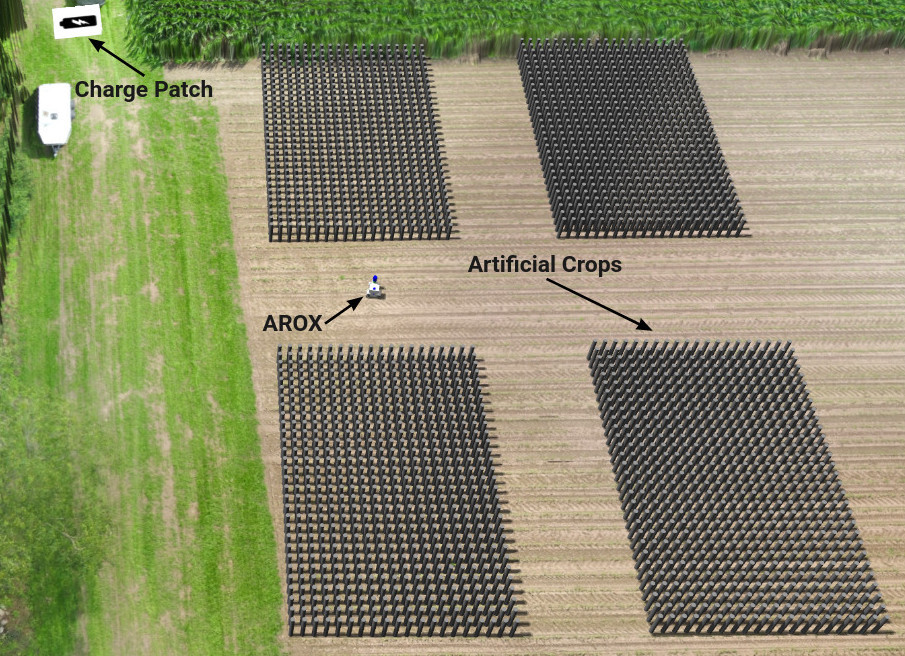
\includegraphics[width=\textwidth]{pics/prototype_scenario.jpg}
        \caption{\textsc{Prototypical Layout}}
        \label{fig:prototypical_layout}
    \end{subfigure}
    \hfill
    \begin{subfigure}[b]{0.49\textwidth}
        \centering
        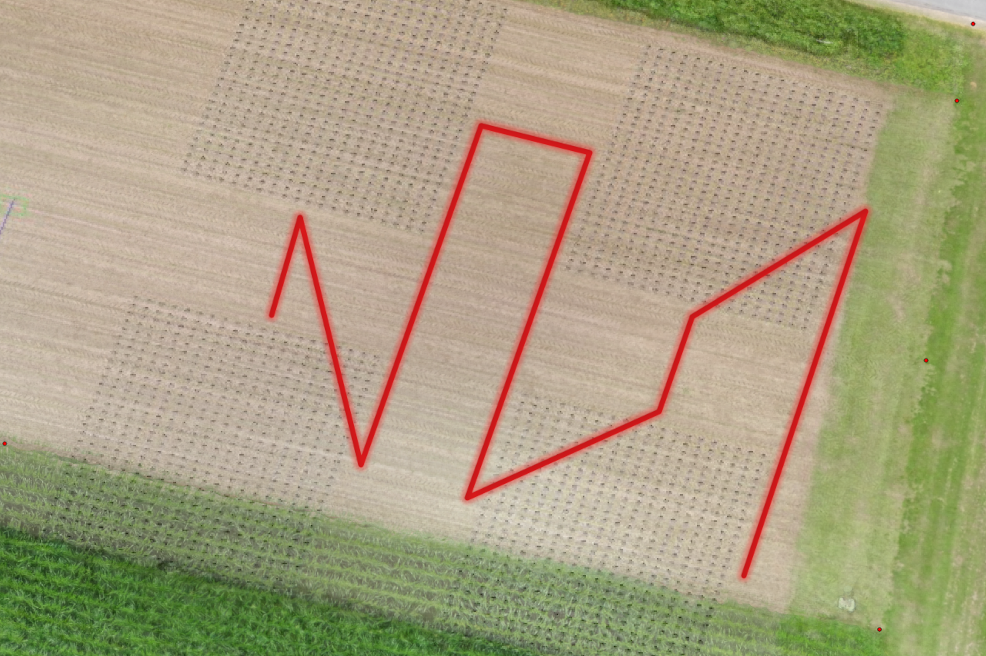
\includegraphics[width=\textwidth]{pics/example_path.png}
        \caption{\textsc{Example Scan Route}}
        \label{fig:example_scan_route}
    \end{subfigure}
\caption{\textsc{Prototype Scenario in the Simulation}}
\label{fig:prototype_sim}
\end{figure}

\section{Robotic System and Infrastructure}
\label{sec:robotic_system}

The robotic system under consideration is going to be the \textit{Autonomous Robotic Experimentation Platform} (AROX) \cite{Kisliuk:2021} that is depicted in figure \ref{fig:arox_system}.
It is assumed to integrate all the essential software and hardware required for the task at hand, i.e. processing a given plan (e.g. human provided) that causes the robot
to autonomously drive to specified locations and record scans. As discussed, this should be possible over extended periods of time, i.e. long term, including charge stops, etc.
According to Kunze et al. \cite{Kunze:2018}, different areas of AI must be brought together to enable long-term autonomous robots in practical applications.
As essential building blocks, they identify \textit{navigation \& mapping}, \textit{perception}, \textit{knowledge representation \& reasoning}, \textit{planning},
\textit{interaction}, and \textit{learning}. Accordingly, all these aspects are in some sense part of the AROX system, some more, some less explicit and sophisticated.
The AROX consists of a two-axle (2WD differential drive) mobile platform based on an \textit{Innok Heros}\footnote{https://www.innok-robotics.de/produkte/heros}. \cite{Kisliuk:2021}
In addition to the AROX system itself, Kisliuk et al. introduce a supporting infrastructure in the form of a mobile base station (container) at the field site,
which provides an inductive charging station, a mobile internet connection and a WiFi network for local data exchange.
Real-time kinematics (RTK) is used, a differential GNSS\footnote{Global Navigation Satellite System} method that results in high-precision positioning (in centimeter range)
near a base station, such as the mobile container. The errors or inaccuracies of basic GNSS techniques are avoided in RTK solutions by transmitting correction signals based
on carrier measurements of the base station, whose location is precisely known. \cite{RTK_fundamentals} For this purpose, the container also provides an NTRIP server.
Besides these technical features of the container, it also simply serves as a shelter for the robot.
In order to actually use RTK, a real-time communication channel (e.g. WiFi) is needed to connect the RTK base station, i.e. the mobile container, with the RTK rover,
i.e. the AROX, to transmit the aforementioned correction signals. Furthermore, it is crucial that both the robot and the base station receive their own GNSS signals, 
i.e. are connected to the GNSS service. The AROX also maintains WiFi or LTE connections for the purpose of transmitting the recorded scans to external servers or the base station.
The robot's localization is multi-layered and based on sensor fusion of inertial measurement unit (IMU), odometry and RTK-GNSS data using the \code{robot_localization} \cite{Moore:2014} package.
Several laser scanners are attached to its base and used to avoid collisions, e.g. the \textit{SICK TiM} and the \textit{Velodyne Puck} mounted at the optional sensor
slots displayed in fig. \ref{fig:arox_system}. For the actual task of plant monitoring, the high-resolution 3D-Lidar sensor \textit{RIEGL VZ-$400$i} is used,
which can be combined with a calibrated hyperspectral or RGB camera (cf. fig. \ref{fig:arox_system}). \cite{Kisliuk:2021}
For \textit{navigation}, the ROS package \code{move_base_flex} \cite{Puetz:2018} is used, a more flexible extension of the standard ROS navigation framework \code{move_base}.
The primarily used path planning algorithms are provided by the ROS packages \code{eband_local_planner} and \code{dwa_local_planner}.
Effective navigation assumes knowledge of the environment, e.g. a map, so that the robot can estimate its position relative to the navigation target. \cite{Krajnik:2010}
There are numerous approaches to representing knowledge about the environment. The map may be static and such that the robot only needs to be able to locate itself in that
map, or the robot may need to perform simultaneous localization and mapping (SLAM). \cite{Krajnik:2010} Particularly in long-term autonomy scenarios, the robot must be able to cope
with environmental changes over time. Santos et al. propose a way for the robot to update and refine its environment representations during long-term application. \cite{Santos:2016}
They introduce a $4D$ environment representation, i.e. they incorporate the time domain to account for dynamic changes. As introduced in section \ref{sec:prototype_scenario}, the AROX
in the basic configuration assumed in this work does not have an explicit \textit{knowledge representation}, but only a predefined static map of the environment. Moreover, the map
is not updated, i.e. no learning takes place in this sense, and no environmental changes are taken into account. In this simple scenario, \textit{reasoning} is also disregarded.
Another interesting facet is \textit{perception}. There is a kind of perception in the form of obstacle detection based on laser scans, but it is not a particularly elaborate form
of perception. An even less pronounced part of the system is \textit{learning}, technically this aspect also occurs somehow, e.g. in the sense that obstacles are detected and entered
into the local costmap. Of course,
sensor information is transferred into a kind of knowledge representation, so in a way obstacles in the environment are learned. Nevertheless, this is not what is typically
understood by machine learning. A counterexample is \textit{interaction}, which is again very explicitly part of the scenario under consideration, namely in the form of communication and
cooperation with the human operator (cf. section \ref{sec:fallback_solution}). The \textit{planning} process itself is not part of the scenario, but it is assumed that plans are available and usable,
e.g. handcrafted by a human operator or generated by a planner from the literature. In further extensions, all these aspects will play a more important role, as useful applications
have already been identified that could improve the long-term autonomy performance of the system in the future, but not in the minimum long-term autonomy scenario considered in this
thesis. To sum up: Technically, all of the aspects proposed by Kunze et al. are somewhat necessary and part of the system, but in part only in a very basal fashion. Certain aspects
are simply not explicitly part of the application. In addition to the actual physically available AROX, the system has been modeled in the unified robot description format (URDF) and
can be used in a simulation.
\begin{figure}[H]
    \centering
    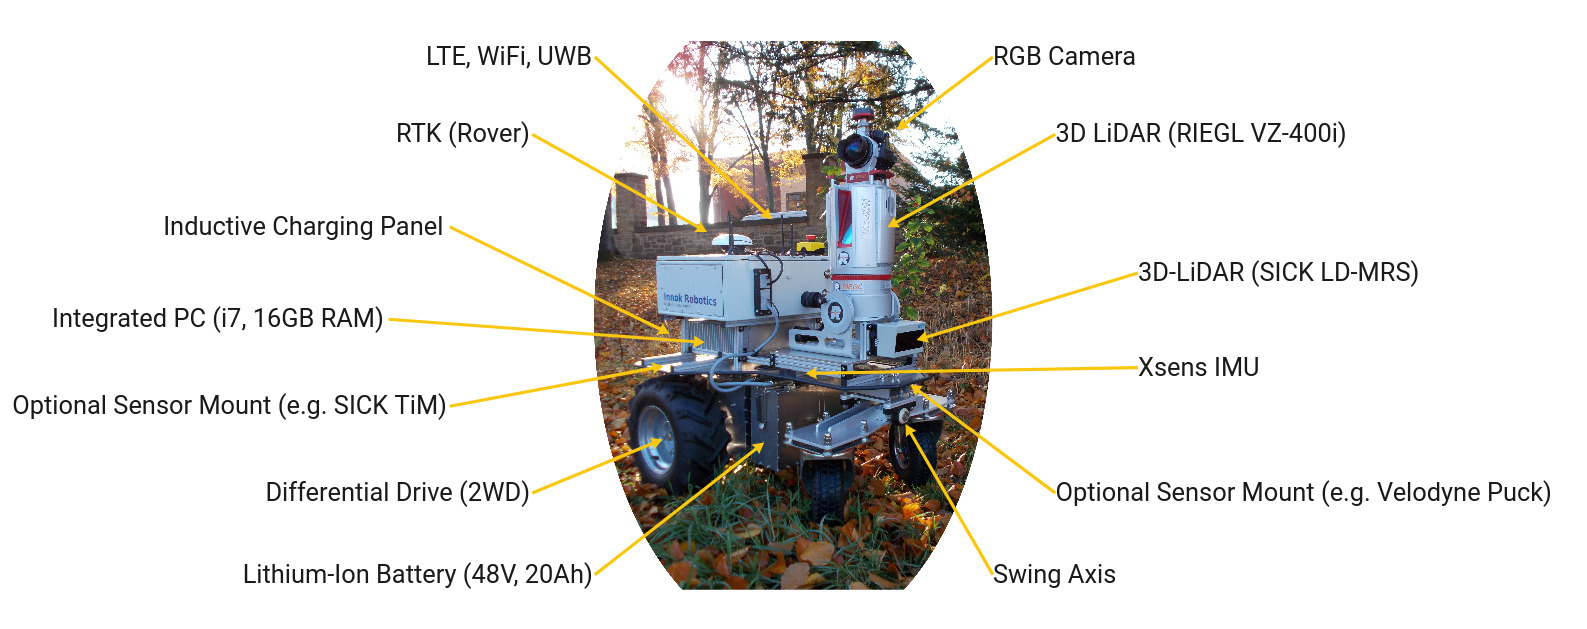
\includegraphics[width=\textwidth]{pics/AROX.jpg}
    \caption{\textsc{Autonomous Robotic Experimentation Platform (AROX)}}
    \label{fig:arox_system}
\end{figure}

\section{Challenges for Long-Term Autonomy}
\label{sec:challenges_for_lta}

Having clarified what long-term autonomy (LTA) means for this work, we now turn to potential problems that stand in its way.
There are numerous potential hinderances for long-term autonomous systems that can cause failure and prevent the system from continuing its task.
The following three constraints precisely define the LTA problems considered in this work.
\begin{enumerate}
    \item It can practically occur in the concrete scenario described in section \ref{sec:lta_plant_observation}.
    \item It can prevent the smooth functioning of LTA systems or affect the quality of its results.
    \item It can be detected by monitoring methods and subsequently solved or communicated.
\end{enumerate}
This definition contains certain implicit assumptions. The first constraint, for example, implies that these problems should have some probability of occurring,
i.e. they should be relatively likely to occur. Accordingly, potential problems such as lightning strikes or wild boar attacks are ignored because they are highly 
unlikely and also difficult, if not impossible, to solve. Moreover, many of the issues of this rather unconventional type, if solvable, could in principle be covered
by more general classes of problems from the following list. Furthermore, the third constraint, i.e. that the considered problems can be detected and subsequently solved 
or communicated, assumes that the system is still fundamentally functioning and has not completely collapsed; a counterexample would again be a lightning strike.
Without claiming to be exhaustive, the following is a list of potential problems in an agricultural field monitoring context that, 
from a practical perspective, fulfill the above restrictions and are thus worthy of investigation:
\begin{itemize}
    \item \textbf{power management} (battery failure / unexpected low battery)
    \item \textbf{charging failure} (unsuccessful docking / no charging)
    \item \textbf{drastic weather change} (e.g. storm, fog, extreme sunshine, heavy rain, extreme cold)
    \item \textbf{certain dynamics} (e.g. day / night)
    \item \textbf{sensor (perception) failure}
    \item \textbf{perceptual aliasing issue}
    \item \textbf{data management} (e.g. full memory, sensor data processing failure)
    \item \textbf{lost connection} (WiFi, GNSS + RTK, LTE)
    \item \textbf{obstacles blocking planned path} (static / dynamic)
    \item \textbf{robot gets stuck} (e.g. spinning wheels)
    \item \textbf{robot falls over}
    \item \textbf{navigation failure} (\code{move_base_flex} / \code{pdc})
    \item \textbf{sustained recovery}, i.e. no return to normal operation
    \item \textbf{incorrect / inaccurate localization} (GPS, IMU, odometry)
    \item \textbf{mapping error} (e.g. incorrect costmap entries)
    \item \textbf{plan deployment failure}, i.e. robot remains in idle state
\end{itemize}
When trying to envision challenges for long-term autonomous application of mobile robots, a common approach is to simply run a robot in such an environment for extended periods
of time and log any information that might somehow be relevant and indicative of problems, e.g. sensor data, internal diagnostics etc. \cite{Biswas:2016}
Some of the problems from the above list result from attempts of this type or the coincidental occurrence in other experiments. Others are obviously potential problems that may occur
and do not require further evidence or justification. The last group is the result of extensive literature research, i.e. challenges encountered in long-term autonomous experiments
presented in the literature. For each potential problem identified, its relevance and consequences, i.e. a brief description of why it might be problematic, is provided below.
A more detailed consideration as well as monitoring and simulation approaches for each selected problem are presented in section \ref{sec:sim_and_mon_of_lta_challenges}.

\subsection{Brief Overview of the Identified Problem Categories}

\noindent
\textbf{Power Management}\newline

\noindent
A natural requirement for LTA systems as defined in section \ref{sec:lta_plant_observation} is some form of energy management.
The system is expected to operate autonomously for extended periods of time, which of course assumes a power supply. 
As Hawes et al. \cite{Hawes:2017} point out, managing consumable resources such as battery charge is critical to long-term autonomous systems.
However, the energy management estimated at planning time may not work correctly or as expected at execution time, e.g. the battery could be 
depleted before the planned time. Or worse, there could be a complete battery failure. It would certainly be useful to enable the system to handle such issues, at least to 
some degree. Arvin et al. point out that long-term autonomy experiments are still rare due to the limited battery capacity of robots. \cite{Arvin:2018}
Therefore, they believe that solving power management issues is of great importance.\newline

\noindent
\textbf{Charging Failure}\newline

\noindent
Another category of potential LTA problems related to the system's power supply is charging failures. Several things can go wrong during a charging process. 
Leaving aside the simplistic assumption of charging upon arrival at specific coordinates and considering the actual charging process 
in practice with the AROX system, it must dock with an inductive charging station in a mobile container at the field site.
Accordingly, docking to the charging station may fail or the charging process itself may not start after docking.
Both cases lead to a failed charging process and thus to an abortion of the robot's LTA mission.
There is evidence in the literature that this is a common problem in long-term autonomous operation of mobile robots. Wang et al. \cite{Wang:2018}, for instance, encountered
this problem during the deployment of their long-term autonomous service robots when the charging port failed and the robot could not recharge and thus continue its mission.
An evaluation of potential docking failures would require integration of the autonomous docking / undocking solution described in section \ref{sec:docking_solution}.\newline

\noindent
\textbf{Drastic Weather Change}\newline

\noindent
Since the AROX system is designed for moderate weather conditions, drastic weather changes can also play a role.
If the weather changes too drastically, it can be problematic for various aspects of the system.
If it is stormy, for example, this can be delicate for the sensor recordings, but also for the robot platform itself, as it could fall over or otherwise be damaged.
The quality of the sensor images can also be affected by fog or extreme sunlight (illumination).
In addition, heavy rain should also be avoided. Finally, extreme cold could be a major problem for the system's battery.\newline

\noindent
\textbf{Certain Dynamics}\newline

\noindent
Similar to weather changes, there are other dynamics such as the natural transition from day to night. For sunlight-dependent sensors such as cameras, 
the robot should take twilight into account and plan its operations accordingly to be back in the shelter, i.e. the mobile container, by dark.\newline

\noindent
\textbf{Sensor (Perception) Failure}\newline

\noindent
Hardware issues are a very general problem class and could relate to almost arbitrary many kinds of problems. Since the correct functioning of the 3D-LiDAR sensor is
crucial for the long-term monitoring scenario described in section \ref{sec:lta_plant_observation}, the main focus will be on detecting hardware faults of this type. 
Sensor failures are, of course, a failure class in which the robot can do little except attempt to restart the corresponding sensor, and therefore rarely has any choice but to 
call the human operator for assistance. Nevertheless, it is important to identify such a malfunction as soon as possible, communicate the problem and avoid a lot of useless work 
and wasted operating time.\newline

\noindent
\textbf{Perceptual Aliasing Issue}\newline

\noindent
Place recognition can certainly be useful for LTA operation of a mobile robot. However, long-term place recognition is not trivial because 
the appearance of places in the environment changes quite drastically over time, e.g. due to illumination, vegetation periods, or weather. \cite{Han:2018}
A useful approach to compare two images (places) is local feature matching, e.g. based on the \textit{Scale-Invariant Feature Transform (SIFT)} and
\textit{Speeded Up Robust Features (SURF)} algorithms. \cite{Valgren:2007} The authors discuss how such approaches can be facilitatd to address the problems related to drastic
environment changes. Another method, proposed by Neubert et al. \cite{Neubert:2013} attempts to predict environmental appearance changes based on the assumption that they are
often systematic and repeatable. Moreover, Latif et al. tackle the task of place recognition using \textit{Generative Adversarial Networks (GANs)}, which enable them to transform the appearance, e.g. from summer
to winter, without requiring knowledge of the image correspondence beforehand, ending up with different versions of an environment snapshot in which the structure remains the same.
\cite{Latif:2018} These versions can then be used to learn how to distinguish locations. A further approach to recognizing changes between observations is based on the idea of
learning to separate the static and dynamic structures of an environment during long-term deployments. \cite{Ambrus:2014}
Visual place recognition in changing environments is a very active area of research, where it is far beyond the scope of this thesis to cover all recent advances (cf. \cite{Porav:2018},
\cite{LowrySur:2016}, \cite{Suenderhauf:2013}, \cite{Lowry:2016}, \cite{Milford:2012}, \cite{Churchill:2013}). In the scenario considered in this work, it is particularly relevant that the robot is able to recognize the place of the mobile container
that serves as shelter and provides the charging station. In addition to the natural changes in the environment over time, there is another important aspect
that makes long-term place recognition particularly challenging - the perceptual aliasing issue. This problem refers to the fact that certain places and objects are very 
similar to each other, that is, they have many common characteristics, which makes them hard to distinguish. \cite{Han:2018}
If, for example, a mobile office container is placed right next to the robot's base station, it might be difficult for the robot to distinguish the objects.
Hence, there could be a need for monitoring methods that are capable of recognizing such situations and providing some strategies to resolve the perceptual aliasing issue.\newline

\noindent
\textbf{Data Management}\newline

\noindent
As robots are deployed for increasingly long periods of time (LTA), it becomes ever more essential to address the challenge of managing the vast amounts of data that are generated
during such deployments. \cite{Ambrus:2014} Since the overall objective of the robot's missions is to acquire data, the appropriate management of this data is of relevance.
If, for example, the robot is no longer able to save further scans due to a full memory, it should recognize and communicate this.
In addition, there may be disturbances in the processing of the sensor data, so that the robot is no longer able to process and save the recordings correctly.
Successful scanning is worthless if the resulting data is not saved properly, so it is important to monitor whether the scans are being written to a file correctly.
Therefore, tt would be valuable to identify such problems as soon as possible to avoid redundant missions.\newline

\noindent
\textbf{Lost Connection}\newline

\noindent
For the robot to work as expected, it must maintain connections to various services. Accordingly, an interruption of one of these connections should be detected immediately.
A real time communication channel (e.g. WiFi) is required to connect the RTK base station, i.e. the mobile container, and the RTK rover, i.e. the robot, in order to
transmit the correction signals for high-precision positioning. In the literature, there are several examples of (semi-)autonomous mobile robots that cannot continue their
mission as expected when they lose WiFi connectivity, such as the service robots considered by Wang et al. \cite{Wang:2018}. The authors also establish a form of network monitoring
to deal with disconnects.
Furthermore, it is crucial that both the robot and the base station receive their own GNSS signals,
i.e. are connected to the GNSS service. Bargoti et al. \cite{Bargoti:2015} and Bechar et al. \cite{Bechar:2016} identify occlusions of GPS satellites leading to jumps in estimated position as one of the main reasons
for detection failures in their tree monitoring scenario, which highlights the value of being able to detect poor GNSS links.
In addition, the RTK-GNSS data is used for scan registration. Finally, the recorded scans are transmitted via WiFi or LTE 
to the base station or external servers for further processing. Whether LTE is behind it or the internet connection is provided via the WiFi connection, it would make sense
to monitor the robot's internet connection in any case. For all connections it is not only about complete disconnects, but also about qualitative estimations.\newline

\noindent
\textbf{Obstacles Blocking the Planned Path}\newline

\noindent
A relatively common problem for the long-term autonomy of a mobile robot is obstacles blocking the planned path.
A rough distinction can be made between static obstacles such as a trailer and dynamic obstacles such as animals or people.
Wang et al. \cite{Wang:2018} even claim that the greatest challenge for the navigation of autonomous robots are dynamic obstacles.
The used navigation framework \code{move_base_flex} can already detect obstacles and initiate a recovery behavior if the planned path is not traversable.
However, it would be good to refine the default recovery behaviors and adapt them to the scenario at hand. In addition, the robot should be able to deal with
recovery failures.\newline

\noindent
\textbf{Robot Gets Stuck}\newline

\noindent
A problem not unlike the obstacles, but slightly different, is that the robot gets stuck and cannot move on. This can happen, for example, when the wheels spin due 
to a muddy path. Such situations where the robot cannot move even though the plan calls for it should be identified and addressed.\newline

\noindent
\textbf{Robot Falls Over}\newline

\noindent
A special case of getting stuck, which should nevertheless be considered separately, is the robot falling over.
This problem should be considered separately, since in such a case the robot will not be able to recover and continue its mission without human assistance in any case.\newline

\noindent
\textbf{Navigation Failure}\newline

\noindent
Another potential LTA problem category, under which a whole range of concrete problems are subsumed, and which have already been encountered in experiments conducted as part of
this work, are navigation errors, which pose a particular challenge in highly dynamic real-world environments. \cite{DelDuchetto:2018}
For example, the local planner configured in \code{move_base_flex} (e.g. DWA, EBand) provides a path that
is infeasible, e.g. tries to drive around a field,  although there is no way. Del Duchetto et al. encounter similar problems in an indoor LTA scenario where valid navigation
trajectories cannot be generated from time to time.
They establish specific, hard-coded ad-hoc recovery behaviors for such cases, ranging from simple wait-and-repeat to interactive human assistance. \cite{DelDuchetto:2018} As Hawes
et al. \cite{Hawes:2017} point out, navigation errors are a critical factor in the long-term autonomy of a mobile robot, as they can result in the robot being incapable of returning
to the charging station (mobile container). Hence, it is imperative to guarantee a certain level of robustness against navigational flaws, i.e. to provide the robot with the
ability to detect and recover from such errors. \cite{DelDuchetto:2018}
The authors define the errors as follows: \textquote{\textit{[...] situation in which the robot is not able to progress toward the goal, because it is not
moving or it is performing some counterproductive behavior}}. \cite{DelDuchetto:2018}
As introduced in section \ref{sec:robotic_system}, the navigation system used is \code{move_base_flex}, an extension of the common ROS navigation framework \code{move_base}.
Navigation issues in practice can be due to a variety of reasons, such as sensor noise, dynamic obstacles, or inaccurate controls \cite{DelDuchetto:2018} and some of them are already
detected by \code{move_base_flex}. Nevertheless, even if this is the case, this information must still be used and processed appropriately by the system in order to be dealt with.\newline

\noindent
\textbf{Sustained Recovery}\newline

\noindent
If the robot tries to recover from a problematic situation, e.g. obstacles on the planned path, such recovery may not be successful, i.e. the robot may not be able
to return to the normal operation state. In case of an unsuccessful recovery attempt, the robot could either give up and abort its mission or perform another recovery.
Of course, the robot should not end up in an infinite loop of repeating the same failing recovery, but instead it should try a few different recovery attempts,
and if none of them work, it should shut down and call the operator. Therefore, it is important to introduce monitoring solutions for recovery behaviors as well.\newline

\noindent
\textbf{Incorrect or Inaccurate Localization}\newline

\noindent
It is obvious that it is a problem when the robot is not able to localize itself correctly in its environment.
Localization is a critical factor for a robot's long-term autonomy, which should therefore not deteriorate during long-term deployments. \cite{Hawes:2017}
In this case, it is a matter of localization within a global reference system, i.e. determining the pose (position and orientation) within a given map of the environment.
If the localization is no longer accurate, e.g. because the robot has been moved to a different position in the map, it must detect this in order to
trigger relocalization. In the case of such a localization error, the \textit{kidnapped robot problem} arises, because although no one has 
physically removed the robot from its position, it appears that way from the robot's perspective. \cite{Hertzberg:2012}
The relevance here can easily be argued based on practical experience, as this issue has already caused a lot of trouble in practice with the AROX system during 
the work for the PORTAL project. In these situations, a major problem for localization was rotating the robot on the spot.
The problems encountered consisted mostly of an incorrect orientation of the robot and rather rarely of an actual incorrect position.
If the orientation is incorrect, the sensor records will also be incorrectly aligned, which is a major problem for the scenario under consideration.
In addition to this practical experience, there are also numerous references in the literature to localization problems in long-term autonomous robot operations. For instance,
Wang et al. \cite{Wang:2018}, who identified localization and execution errors as the two core problems in their long-term application of indoor service robots.
They identify unexpected changes in the robot's position estimates as a useful method for predicting / detecting localization problems.
Of course, it can also be a problem for localization if the GNSS signal itself is inaccurate or non-existent \cite{Churchill:2013}, but that is another topic (cf. \textit{Lost Connection} section).
There are arbitrary many potential localization problems (e.g. slipping in sand, getting stuck, jammed wheels) and the correct functioning of the system always assumes an accurate
position estimate. \cite{Goldberg:2002}

\vfill
\pagebreak

\noindent
\textbf{Mapping Issues}\newline

\noindent
Mapping issues can generally refer to a variety of problems. In this case, a particular issue regarding the local \textit{costmap} observed during experiments for this work is meant.
The \textit{costmap} is a 2D occupancy grid based on sensor data of the world. It generates costs based on a user defined inflation radius.
If the robot drives over a hill and the sensors are configured in a certain way, parts of the ground may be incorrectly perceived as an obstacle and entered into the \textit{costmap}.
The problem then is that the robot is unable to drive through these ``virtual'' obstacles. \newline

\noindent
\textbf{Plan Deployment Failure}\newline

\noindent
The last type of problem is rather trivial again. If the plan distribution node does not provide a plan for the robot to execute, it remains idle until a human operator 
notices and takes care of it. It might therefore be useful to let the operator know if a plan has still not arrived after a certain time.
In addition, faulty plans that are not executable should also be reported, which requires some kind of content plausibility check.\newline

\noindent
\textit{Concluding Remarks.}\newline

\noindent
The idea is to tackle a subset of this list of issues that is realistically solvable in the scope of the work.
Generally, the potential barriers for long-term autonomy can be classified into three categories of increasing negative impact on the system:
\begin{figure}[H]
\centering
\begin{enumerate}
    \item The robot recognizes a problem and is able to solve it by itself.
    \item The robot recognizes a problem, is unable to solve it, and calls a (human) operator for help.
    \item The robot has a malfunction / problem, but does not recognize it and is therefore unable to solve or communicate it.
\end{enumerate}
\caption{Classification of Problems in Terms of Impact}
\label{fig:problem_types}
\end{figure}
Type $(1)$ is the ideal case and accordingly the ultimate goal of all efforts to implement long-term autonomy in practice. Type $(2)$ is already a step forward, because problems
are at least recognized and can be communicated, which is the minimum requirement to guarantee a certain robustness with respect to the problems.
In the baseline scenario, i.e. the running prototype of an integrated solution, each potential issue in the above list is classified as type $(3)$.
Part of the goal of this work is to shift the problems of the selected subset to another category and thereby improve the utility of the system, 
i.e. to solve them completely $(1)$, or at least to enable the robot to recognize them with execution monitoring approaches and request help $(2)$.
However, it is also part of the truth that not all possible external influences are solvable, i.e. a robot will not be able to solve all
conceivable problems itself. Long-term autonomy has its limits, and there are simply unpredictable situations that a mobile robot cannot be expected to handle,
e.g. if its battery bursts into flames, or it is knocked over by something. In such a case, the only way to do damage control is to try to shut down the 
robot in a controlled manner (e.g. with data backup) and, if possible, communicate the problem.
Of course, one could assign probabilities to specific incidents, which vary depending on the information available. 
For example, if the robot detects that the battery is showing unusual discharge behavior, such information could be taken into account and 
reported to the operator. Nevertheless, it's not feasible to cover everything that can happen, and long-term autonomy is subject to certain limits.

\subsection{Relevance Assessment}
\label{sec:relevance_assessment}

To assess the relevance to long-term autonomy of the potential problems introduced in the last section, a kind of informal analysis of the impact, 
difficulty, and likelihood of each problem was conducted. The idea is not to arbitrarily select the problems that will be studied in more detail as part
of this work, but to rely on the judgment of the more experienced roboticists in the working group, especially those who have hands-on experience with the
AROX or similar systems, to set priorities. For this purpose, a simple questionnaire was designed in the form of a spreadsheet. The first aspect by which participants 
were asked to rank each problem was its respective impact from \textit{high} ($1$), i.e. prevents a successful mission, to \textit{medium} ($2$) impact, e.g. delays missions 
or reduces the quality of results, to \textit{low} ($3$), where it has at most a minor impact on the robot's mission. The next aspect was about evaluating each problem in 
terms of its individual difficulty of solution and recognition. The options were \textit{easy} ($1$), meaning that simple solutions exist, \textit{medium} ($2$), which 
requires some effort but should be feasible within the scope of the work, to \textit{hard} ($3$), i.e. that it is a rather general problem that can only be tackled in first 
approximation. Finally, the likelihood of each problem occurring should be evaluated using the following three options. \textit{Very likely} ($1$), which roughly means you
have experienced this in practice several times, \textit{occurs} ($2$), meaning you have experienced or heard of this once, and \textit{highly unlikely} ($3$), meaning 
you have never seen or heard of this. The questionnaire was completed by a total of $7$ people. Obviously, this can by no means be considered representative or significant, but it 
nevertheless does give an indication of which problems should be considered with higher priority and contributes to systematization. The accumulated results are visualized in the
3D scatter plot depicted in figure \ref{fig:questionnaire_results}. For each problem, the average vote among all three dimensions (impact, difficulty, likelihood) is displayed.
The most relevant problem to consider under the introduced scoring system would be a problem at coordinates $(1, 1, 1)$, i.e. a high-impact problem 
that is easy to solve / discover and has a high probability of occurring. This optimal combination is shown as a golden cross in figure \ref{fig:questionnaire_results}.
The problems closest to this point in 3D space are the ones that are most important to consider based on the questionnaire and therefore should be 
investigated with higher priority in this work. For a more detailed overview, the average results and each problem's distance to the optimum can be taken from the table 
in figure \ref{fig:average_results}.
\begin{figure}[H]
    \centering
    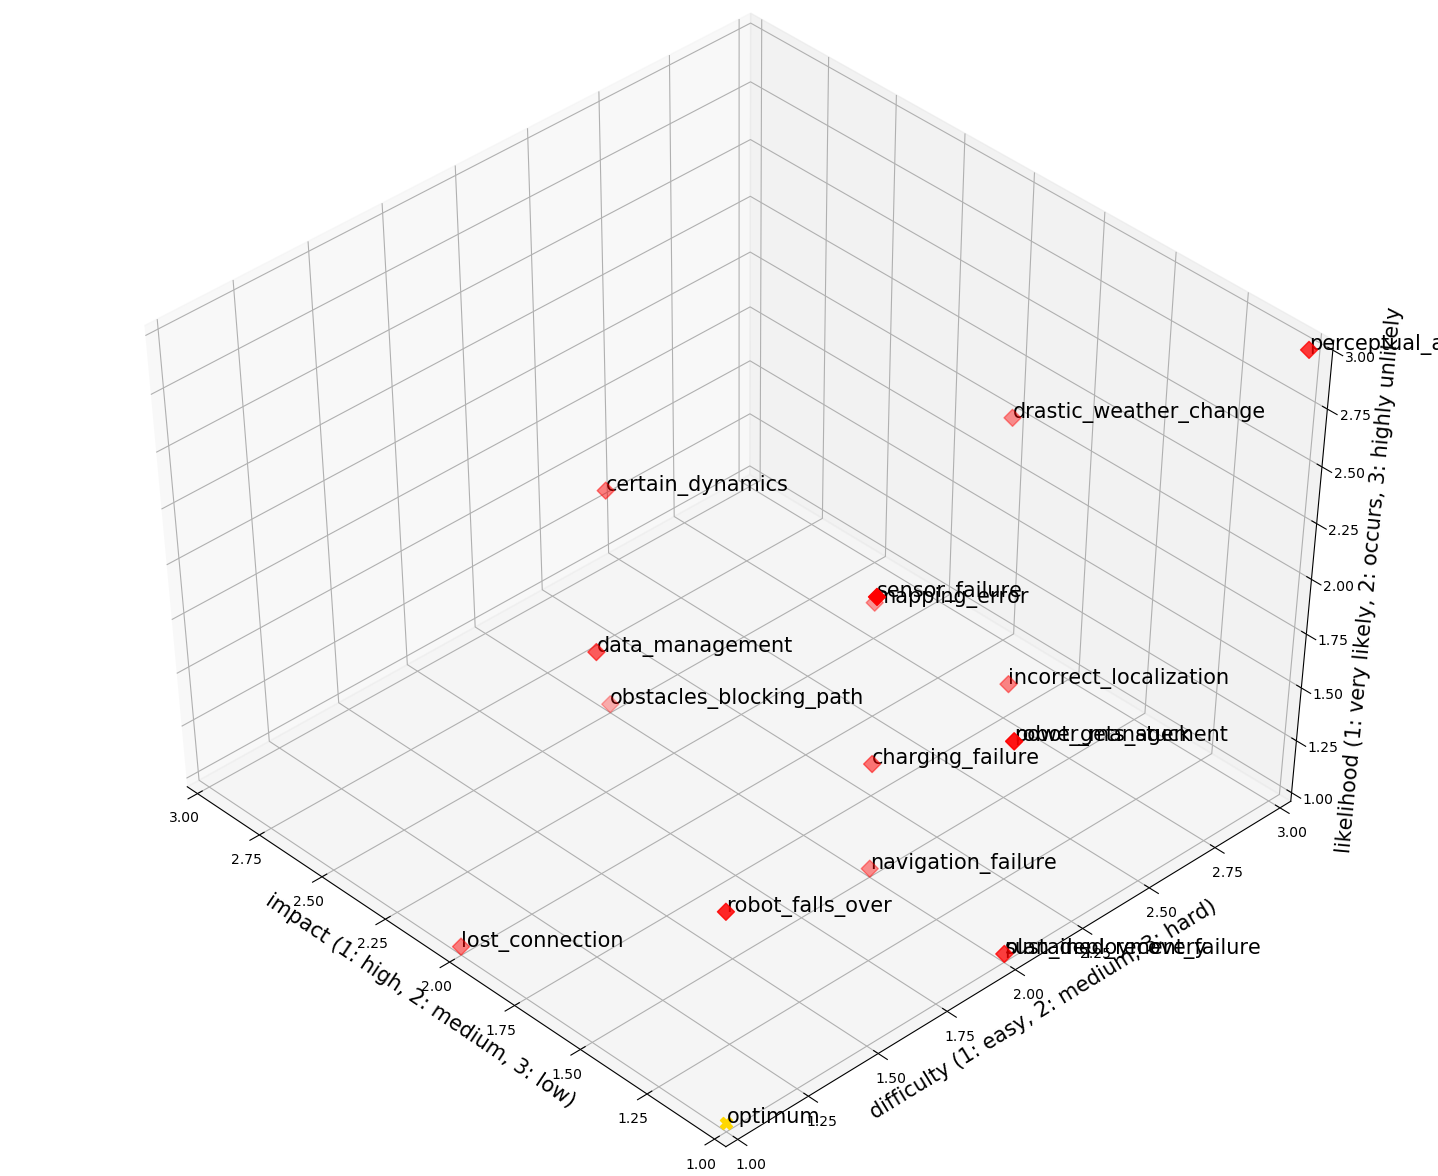
\includegraphics[width=0.95\textwidth]{pics/questionnaire.png}
    \caption{\textsc{Accumulated Results of Questionnaire}}
    \label{fig:questionnaire_results}
\end{figure}
\noindent
The results shown in the table in fig. \ref{fig:average_results} are ordered by their relevance according to the questionnaire results, i.e.
by their distance from the optimal combination of impact, difficulty, and likelihood. It is worth mentioning, however, that the resulting order is based on the assumption
that the three criteria of impact, difficulty, and likelihood are equally important in the consideration. One could argue that the difficulty criterion was introduced 
primarily because of the tight time frame of this work and may be less important when it comes to the question of which problem is really crucial to solve in practice.
Thus, it is worth considering the two-dimensional results only in terms of the expected impact and likelihood of each problem displayed in fig. \ref{fig:questionnaire_results_2d}.
\begin{figure}[H]
    \centering
    \resizebox{0.75\textwidth}{!}{
    \begin{tabular}{| c | c | c | c | c |}
        \hline
        \textbf{problem} & \textbf{\o \thinspace impact} & \textbf{\o \thinspace difficulty} & \textbf{\o \thinspace likelihood} & \textbf{dist. to optimum} \\ \hline
        charging\_failure & $1.29$ & $1.29$ & $1.71$ & $0.82$ \\ \hline
        power\_management & $1.0$ & $1.43$ & $2.0$ & $1.09$ \\ \hline
        data\_management & $1.57$ & $2.0$ & $1.86$ & $1.44$ \\ \hline
        sensor\_failure & $1.57$ & $1.71$ & $2.14$ & $1.46$ \\ \hline
        incorrect\_localization & $1.57$ & $2.29$ & $1.57$ & $1.52$ \\ \hline
        lost\_connection & $2.14$ & $1.86$ & $1.57$ & $1.54$ \\ \hline
        navigation\_failure & $1.86$ & $2.0$ & $1.83$ & $1.56$ \\ \hline
        plan\_deployment\_failure & $1.67$ & $1.83$ & $2.17$ & $1.58$ \\ \hline
        mapping\_error & $1.86$ & $2.14$ & $1.71$ & $1.6$ \\ \hline
        certain\_dynamics & $2.43$ & $1.43$ & $1.71$ & $1.65$ \\ \hline
        obstacles\_blocking\_path & $2.29$ & $2.14$ & $1.43$ & $1.77$ \\ \hline
        robot\_gets\_stuck & $1.43$ & $2.29$ & $2.14$ & $1.77$ \\ \hline
        sustained\_recovery & $1.33$ & $2.5$ & $2.0$ & $1.83$ \\ \hline
        drastic\_weather\_change & $1.86$ & $2.43$ & $2.29$ & $2.11$ \\ \hline
        robot\_falls\_over & $1.0$ & $2.33$ & $2.67$ & $2.13$ \\ \hline
        perceptual\_aliasing\_issue & $2.0$ & $2.5$ & $2.33$ & $2.24$ \\ \hline
    \end{tabular}}
\caption{\textsc{Results of the Evaluation - Problems Ordered by Relevance}}
\label{fig:average_results}
\end{figure}
\begin{figure}[H]
    \centering
    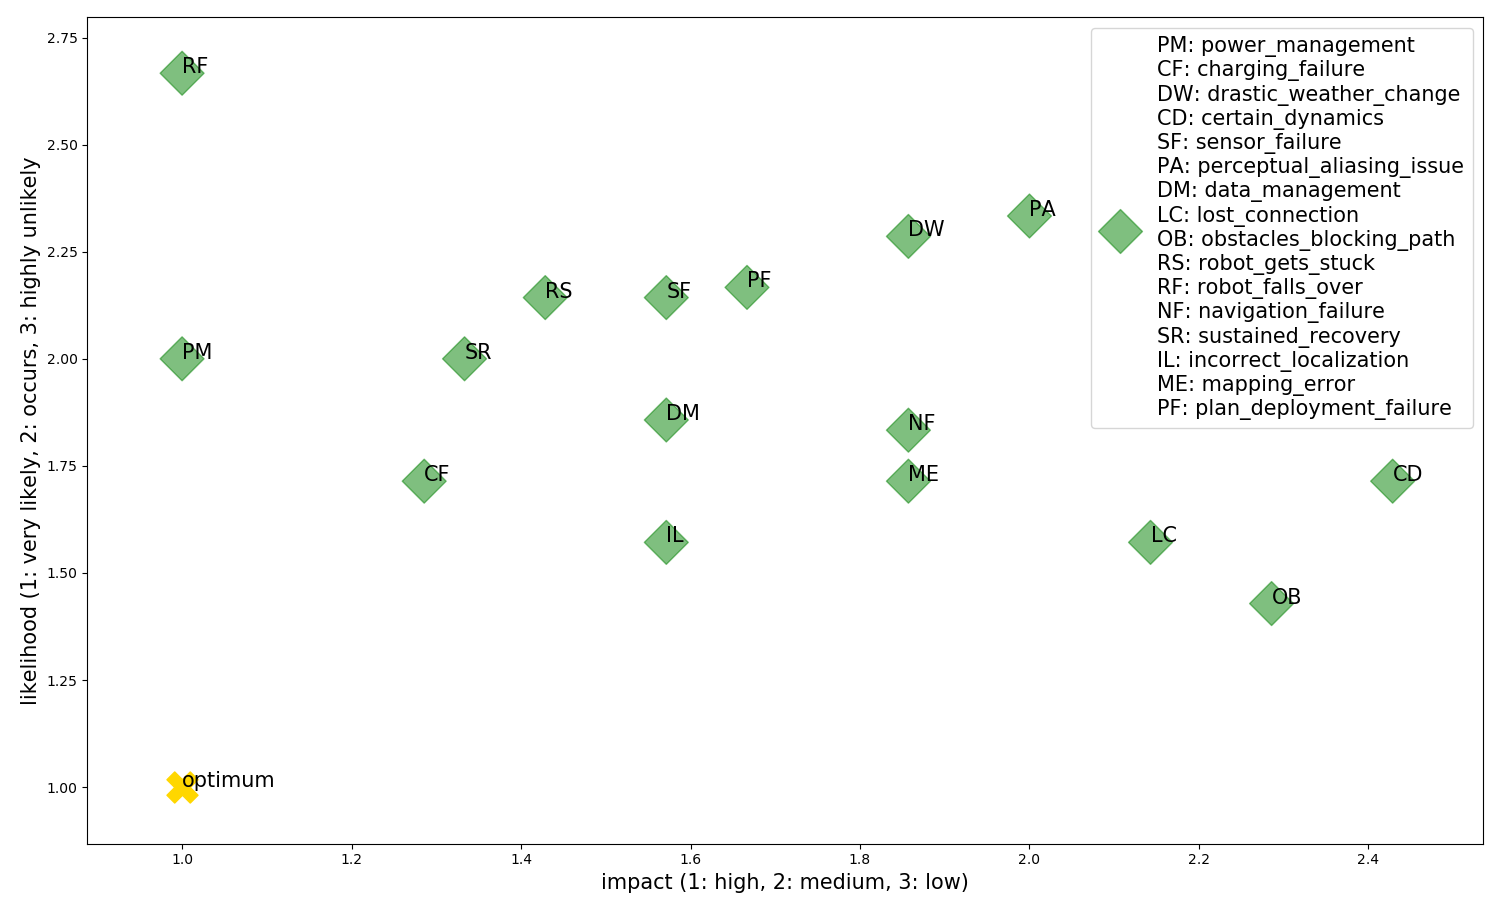
\includegraphics[width=0.7\textwidth]{pics/questionnaire_2d.png}
    \caption{\textsc{2D Results of Questionnaire}}
    \label{fig:questionnaire_results_2d}
\end{figure}
\noindent
Another interesting aspect to analyze is the range in given answers in the questionnaire, i.e. the agreement among the participants. Most of the judgments roughly coincide with
only few outliers. However, there are some controversial cases that are worth mentioning. First, the \textit{impact} category seems to be the easiest to assess, as it is the only
one where all participants agreed on two problem types (power management, robot falls over). In addition, the other problem types in the \textit{impact} category are rated fairly
consistently, most of them have only one outlier vote, and it is very rare that the votes are completely mixed. The most contested problem types in this category are perceptual
aliasing, connection losses, situations where the robot gets stuck, and navigation failures. It is also interesting to examine the reason for the mixed results. This could be
because most participants rated the problem as average on the scale, but it could also arise from extreme answers canceling each other out. There's a big difference - one means
participants agree, the other means they do not. For the \textit{impact} category, participants seem to agree overall, with only a few outliers and even some cases of perfect
agreement with unanimous votes. The next category, \textit{difficulty}, is already not so clear-cut, which may be explained by the fact that participants could imagine different
depths of problem-solving based on their particular experience, while \textit{impact} is quite easy to think about. There is no unanimous vote, and there are even some cases where
the answers are very mixed, such as in the case of lost connections, where the answers are almost evenly distributed among the possible options. However, this is still rare, in most
cases the overall trend is clear. Finally, the voting in the third category \textit{likelihood} is similar to the \textit{difficulty} votes. There is no unanimous vote, but there
are cases where participants are pretty much in agreement, such as in data management failures, where all but one voted for $2$ (\textit{occurs}). There is no extreme example of
evenly distributed responses, most have some tendency and a few outliers. In summary, an average score almost never results from an even distribution of responses across the options,
but almost always results from the actual rating of the problem as average based on the criteria. The exact results can be taken from the appendix 
(cf. \ref{sec:detailed_questionnaire_results}). As shown in fig. \ref{fig:average_results_2d}, the $2D$ evaluation purely based on impact and likelihood results in a different ordering based on their distances 
to the $2D$ optimum $(1, 1)$.
\begin{figure}[H]
    \centering
    \resizebox{0.65\textwidth}{!}{
    \begin{tabular}{| c | c | c | c | c |}
        \hline
        \textbf{problem} & \textbf{\o \thinspace impact} & \textbf{\o \thinspace likelihood} & \textbf{dist. to optimum} \\ \hline
        charging\_failure & $1.29$ & $1.71$ & $0.77$ \\ \hline
        incorrect\_localization & $1.57$ & $1.57$ & $0.81$ \\ \hline
        power\_management & $1.0$ & $2.0$ & $1.0$ \\ \hline
        data\_management & $1.57$ & $1.86$ & $1.03$ \\ \hline
        sustained\_recovery & $1.33$ & $2.0$ & $1.05$ \\ \hline
        mapping\_error & $1.86$ & $1.71$ & $1.12$ \\ \hline
        navigation\_failure & $1.86$ & $1.83$ & $1.2$ \\ \hline
        robot\_gets\_stuck & $1.43$ & $2.14$ & $1.22$ \\ \hline
        sensor\_failure & $1.57$ & $2.14$ & $1.28$ \\ \hline
        lost\_connection & $2.14$ & $1.57$ & $1.28$ \\ \hline
        plan\_deployment\_failure & $1.67$ & $2.17$ & $1.34$ \\ \hline
        obstacles\_blocking\_path & $2.29$ & $1.43$ & $1.36$ \\ \hline
        drastic\_weather\_change & $1.86$ & $2.29$ & $1.55$ \\ \hline
        certain\_dynamics & $2.43$ & $1.71$ & $1.6$ \\ \hline        
        robot\_falls\_over & $1.0$ & $2.67$ & $1.67$ \\ \hline
        perceptual\_aliasing\_issue & $2.0$ & $2.33$ & $1.67$ \\ \hline
    \end{tabular}}
\caption{\textsc{Results of the $2D$ Evaluation - Problems Ordered by Relevance}}
\label{fig:average_results_2d}
\end{figure}
\noindent
First, it is interesting to note that the charging failure is undisputedly in first place in both the two-dimensional and three-dimensional evaluations.
The problem of incorrect localization climbs to second place if the difficulty criterion is disregarded. This is followed, as before, by power and data management.
Subsequently, sustained recovery makes a huge jump of eight places when leaving aside its assumed difficulty to detect and solve.
Mapping errors are also on the rise, overtaking sensor failures, lost connections, navigation failures, and plan deployment errors.
Another interesting aspect is that sensor failures are far less relevant when disregarding their surprisingly low rated difficulty.
The remaining problems remain broadly similar in their assessment, with some changing places in the middle of the list, but this is not so relevant.
The problems rated as least relevant in the questionnaire remain the same as in the 3D case, mainly because they are considered relatively unlikely.
In conclusion, both lists are used to prioritize the problems to be studied in this work, as it is of course useful to also consider the difficulty of 
solving these problems, but the $2D$ view can be helpful in case of doubt.\newline

\noindent
\textbf{Systematization of LTA-Challenges}\newline

\noindent
It would be beyond the scope of this work to tackle every identified potential challenge for a mobile robot's long-term autonomy. Therefore, it is necessary to select a subset of the
problems to be considered based on the results of the questionnaire. For this subset, monitoring methods are presented that do not necessarily solve $100\%$ of the possible cases,
but a certain fraction, at least to a first approximation. In addition, more fundamental problems are emphasized that cannot be addressed in general within the scope of this work;
special cases may be. 
First, it is obvious that charging failures should be addressed in this work, since they are undisputedly in the first place in both the two-dimensional and three-dimensional
evaluations of the questionnaire (cf. \ref{sec:sim_and_mon_charging_failures}). Thematically closely related and also very relevant based on the survey:
power management problems (cf. \ref{sec:sim_and_mon_power_management}). Another aspect high on the list to be considered in this work is data management
issues (cf. \ref{sec:sim_and_mon_data_management}). Furthermore, sensor (perception) failures are a class of problems that should not be ignored in this work
(cf. \ref{sec:sim_and_mon_sensor_failures}). Although in principle a very intricate and general class of problems, localization issues, i.e. incorrect
localization (cf. \ref{sec:sim_and_mon_incorrect_localization}), has to be considered in this work, especially due to its high impact and likelihood
that can be seen in fig. \ref{fig:average_results_2d}. Additionally, connection problems are treated (cf. \ref{sec:sim_and_mon_lost_connections}). Also quite
general, but pretty high on the list are navigation errors, which are taken into account at least to some degree (cf. \ref{sec:sim_and_mon_navigation_failures}). Being relatively easy to detect, plan deployment failures will be tackled as well (cf. \ref{sec:sim_and_mon_plan_deployment_failures}). Although the problem of obstacles blocking the robot's path is ranked quite low in the lists in figs. \ref{fig:average_results} and
\ref{fig:average_results_2d}, it is considered to some extent because the reason for its low ranking is mainly its relatively small impact. However, it is rated as very likely,
and it would be good if such situations could be dealt with effectively (cf. \ref{sec:sim_and_mon_navigation_failures}). The problem of sustained recovery is fairly low on
the list in the $3D$ assessment, but very high in the $2D$ case, mainly because of its relatively large impact. Thus, it will be studied (cf. \ref{sec:sim_and_mon_navigation_failures}). The issue of drastic weather changes is rated as rather irrelevant in the overall result of the questionnaire. However, this is mainly due to
its high rated difficulty and the relatively low likelihood. Although it may be difficult to solve in general, it will be dealt with in first approximation due to its quite high
impact (cf. \ref{sec:sim_and_mon_drastic_weather}).\newline
A not so high-rated and also very general problem class that is not considered in detail in this work: Mapping errors. The problem class ``certain dynamics'' is of course formulated
quite generally in the questionnaire, which could be one of the reasons for the low impact rating, but for this work dynamics like sunset are not further investigated as they are
quite predictable. In addition, situations in which the robot gets stuck are not taken into account because they are regarded relatively irrelevant due to their low probability.
Of course, it is a severe problem when it happens, but the robot actually getting completely stuck is relatively rare, and due to the many possible reasons for getting stuck, 
a very general problem class. All participants agree that the scenario where the robot topples over has a very large impact, but it is also quite difficult to detect and quite
unlikely. It is not studied in detail itself, but might be detected as part of the sensor failure detection, e.g. if the sensor subsequently points to the sky (cf.
\ref{sec:sim_and_mon_sensor_failures}). Finally, ranked as least relevant in both evaluations, perceptual aliasing issues will be disregarded in this work. The problems not examined in
detail in this thesis are nevertheless potentially relevant problems for the long-term autonomy of a mobile outdoor robot and are thus briefly discussed in section 
\ref{sec:lta_problems_not_considered}.

\pagebreak

\subsection{Disregarded Problem Categories}

\label{sec:lta_problems_not_considered}

TODO: Clean up / refine section..\newline

\noindent
\textbf{Certain Dynamics}\newline

\noindent
There should be a monitoring solution that is able to detect twilight, stop the plan execution and postpone it to the next day.
It should be possible to simulate twilight in the \textit{Gazebo} simulation, e.g. by simply dimming the light source.\newline

\noindent
\textbf{Perceptual Aliasing Issue}\newline

\noindent
There could be a need for monitoring methods that are capable of recognizing such situations and providing some strategies to resolve the 
perceptual aliasing issue., e.g. by changing the position or the viewpoint in order to discriminate the objects.
The occurrence of a perceptual aliasing issue can be simulated, for example, by placing an object similar to the container in the simulation.\newline

\noindent
\textbf{Robot Gets Stuck}\newline

\noindent
Detection should be based on \code{move_base_flex} recovery behaviors, as in the case of obstacles, but again there should be a manual implementation 
specifically for these cases where, for example, the robot tries to rotate and reduce speed to leave the place where it got stuck.
In simulation, such a situation could be established by providing the necessary physical conditions leading to such a problem.\newline

\noindent
\textbf{Robot Falls Over}\newline

\noindent
It could be tested in simulation by applying a force to the robot that causes it to fall over.
It should be possible to detect the problem based on a combination of sensor information, and the robot should notify the human operator.\newline

\noindent
\textbf{Mapping Issues}\newline

\noindent
It is demanded to either pay close attention to obstacle detection when moving on uneven terrain or to clear the \textit{costmap} from time to time
to eliminate such erroneous entries. This is especially true for recovery behaviors,  where such ``virtual'' objects can block a path that the robot must traverse.
The problems described can be evaluated in simulation by having the robot travel over rough terrain or by artificially creating paths with steep inclines.

\chapter{Plan Execution and Monitoring}
\label{sec:plan_execution_and_monitoring}

Ghallab et al. point out several types of deliberation functions required for the successful deployment of autonomous artificial agents in diverse environments,
such as \textit{planning}, \textit{acting}, \textit{monitoring}, \textit{goal reasoning}, \textit{reasoning about sensing and information gathering}, and \textit{learning}. \cite{GNT:2016} This chapter deals with arguably the most
fundamental - \textit{planning}, \textit{acting} and \textit{monitoring}. Although, it is not about the plan generation itself, but rather about the handling and execution of given plans.
A key aspect of dealing with some of the potential issues introduced in section \ref{sec:challenges_for_lta} is going to be that the robot will not be able to
complete its missions without preempting the plan execution from time to time. Either due to insufficient battery capacity or other unmanageable conditions such as 
drastic weather changes that force the robot to interrupt its task. As Harris et al. remark: \textquote{\textit{Fixed plans may fail if states encountered during execution do not
sufficiently reflect the assumptions made during plan generation}}. \cite{Harris:2021} Although the overall route may always be the same for the same field, there are certain stopping
conditions that cause the robot to interrupt its active scanning tour and possibly drive back to its base, i.e. the mobile container.
There are generally two relevant perspectives. First, such stops have to be considered at planning time by acknowledging charge stops as crucial part of the plan.
Of course, this is only covering plannable stops such as expected battery consumption and is not able to deal with unplanned situations.
Therefore, a second perspective comes into play, that will be particularly relevant in this work - the execution time.
Just as important as the planning itself is the execution of the generated plan as well as monitoring the execution. Execution monitoring enables a robotic system to
recognize and classify failure situations caused by unexpected internal (robot) or exteral (environment) states. \cite{Pettersson:2005}
The idea is that the robot executes a given plan and is somehow capable of realizing that it has to interrupt the execution due to some unexpected condition.
In such a case, the robot needs to be able to save the current state of the plan execution and continue precisely with this state after the reason 
for the interruption has been resolved. Consequently, the robot has to be prepared to pause and resume the execution of a given plan, which is far from 
trivial, since the original plan may no longer be applicable for various reasons. This aspect is discussed further in section \ref{sec:plan_interruption_section}.
In this work, \textit{monitoring} is not meant to monitor plan execution in the sense of evaluating
pre- and post-conditions of specific high-level actions and the like, but is to be understood in a more general sense to monitor aspects of the robot system as well as its environment
that have been identified as critical to successful long-term autonomous deployment (cf. \ref{sec:challenges_for_lta}). Essentially, the things that are implicitly part of the plan,
like working sensors and a reasonable battery state of charge. \cite{Ingrand:2017} Based on the challenges identified in section \ref{sec:challenges_for_lta}, this includes the use of
proprioceptive as well exteroceptive sensors and information. As Hawes et al. put it: \textquote{\textit{A key strategy for
delivering long-term robustness is the monitoring of system behavior, from the individual component level up to navigation and task behaviors, as well as the ability to restart
system elements on demand}}. \cite{Hawes:2017} Likewise, Furgale et al. assert that long-term autonomous robots need introspection capabilities to recognize internal problems in
the interest of safety. \cite{Furgale:2015} Ingrand et al. perfectly summarize the view of monitoring in this work: \textquote{\textit{Compares what is predicted regarding the robot
activities to what is observed in the world. It detects and interprets discrepancies, performs diagnosis and triggers recovery actions when needed.}} \cite{Ingrand:2017}
As with planning, monitoring always raises the question of the level of the robot architecture at which it is carried out. The idea of this thesis is essentially to do it at an abstract level
defined by the rough notion of being as universal as possible to achieve some form of reusability while being applicable and useful in the context under consideration. Obviously,
monitoring also takes place at other levels of abstraction, such as monitoring WiFi signal strength or monitoring within \code{move_base_flex}, which reports errors. There is simply
no fundamental answer to the question of where monitoring should take place. Presumably, one could break it down to the fact that monitoring is necessary at all levels of abstraction,
at least in the sense of error treatment.
The potential problems identified in section \ref{sec:challenges_for_lta}, and their subtypes, are generally classified into two categories in this thesis according to their severity:
Those that cause contingencies and those that lead to catastrophes. The essence of these two categories has already been anticipated by the first two classes of problems in the
concluding remarks of section \ref{sec:challenges_for_lta}. Contingencies refer to cases where the robot is confronted with an unexpected event or problem, but its ability to act is
basically preserved, so that it can try to solve the problem itself, e.g. by returning to base. Catastrophes, on the other hand, refer to cases where the robot is no longer capable of
acting or solving the problem, necessitating human intervention. It is roughly equivalent to the definition of Ross et al. described in \cite{Honig:2018}, where
failures are divided into anticipated errors, exceptional errors, and unrecoverable errors based on the recoverability of the system. The ideas are more based on a high-level planning
perspective, as the first two refer to simple backtracking and replanning, respectively, while the last refers to cases where the plan is no longer feasible and replanning is not an
option. Nevertheless, the first two in combination correspond quite well to the view of contingencies in this thesis - contingencies can be dealt with. Similarly, unrecoverable errors
correspond to catastrophes in this work. They also consider socially recoverable failures where the robot relies on assistance from other operators (humans or other robots), which
is also encountered in this work, namely in the case of the catastrophe situations (cf. section \ref{sec:fallback_solution}).

\section{Plan Generation and Format}
\label{sec:plan_generation}

Long-term autonomous robot operation commonly includes following some sort of plan $\pi$. Planning is the process of selecting and ordering actions that must be performed to
achieve an objective. \cite{GNT:2016} While actions generally refer to processes that change the state of the robot or its environment, they can be considered at different
levels ob abstraction. \cite{Ingrand:2017} However, since the actual planning is not part of this work, it is assumed that
plans are provided and usable, e.g. handcrafted by a human operator or generated by a planner from the literature.
For the purpose of parsing a plan $\pi$ and making it retrievable via a service call, a ROS node was developed.
In order for the node to parse the plans, they must be formulated in the following CSV format.
Let $A := \{$\code{drive_to(lat, lng, theta)}, \code{return_to_base}, \code{charge}, \code{scan}$\}$ be the set of available actions in the considered scenario
described in section \ref{sec:prototype_scenario}.
Each line in a provided CSV file represents one action $a \in A$ of a plan $\pi$. The actions \code{return_to_base}, \code{charge} and \code{scan} have no parameters,
but \code{drive_to(lat, lng, theta)} needs the additional arguments latitude ($lat$), longitude ($lng$), and orientation ($\theta$) of the target pose. As anticipated in section
\ref{sec:prototype_scenario}, \code{drive_to(lat, lng, theta)} causes the robot to drive to the specified latitude and longitude, and take the specified
orientation. Analogously, \code{return_to_base} directs the robot to move to a user-configurable base position. \code{charge} in the simplified case with the charging patch is simply
a call that charges the battery when the robot is located at the corresponding coordinates. Leaving aside the simplifying assumption of charging at the charging station presented in
section \ref{sec:prototype_scenario} and considering the realistic case with the container infrastructure (cf. \ref{sec:docking_solution}), there are two other implicit actions
- \code{dock} always follows \code{return_to_base} and lets the robot dock to the inductive charging station inside the container and \code{undock} follows \code{scan} and reverses
the docking procedure. Finally, \code{scan} initiates a scanning operation at the robot's current position, using either the RIEGL sensor in practice or the dummy node (cf. section
\ref{sec:dummy_scanning_node}) in simulation, which saves a simulated \code{LaserScan} or \code{PointCloud2} to disk, depending on the configuration.
An example for a simple plan is shown in figure \ref{fig:plan_example}.
When the robot executes this plan, it drives to the four specified locations in sequence and records scans.
Afterwards, it returns to the base and recharges its battery. However, acting requirers a lot more than only processing abstract actions provided by a plan (cf. 
\ref{sec:execution_monitoring_smach_architecture}). \cite{Ingrand:2017}
\begin{figure}[H]
    \centering
    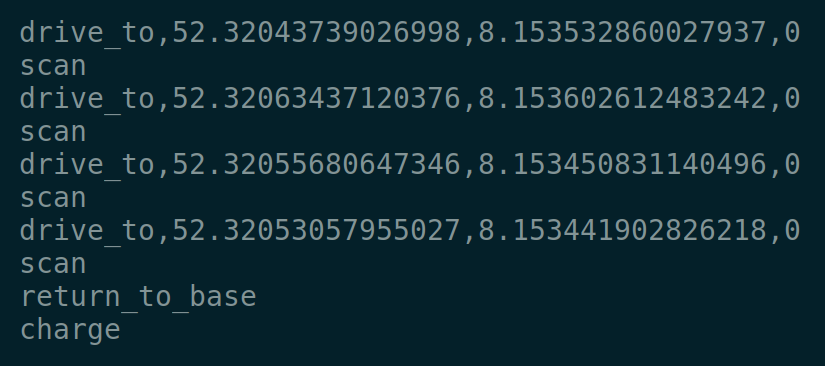
\includegraphics[width=0.5\textwidth]{pics/plan_example.png}
    \caption{\textsc{Sample Plan}}
    \label{fig:plan_example}
\end{figure}
\noindent

\section{Execution Monitoring State Machine Architecture}
\label{sec:execution_monitoring_smach_architecture}

Before introducing the developed architecture for plan execution, i.e. acting, and monitoring, it is useful to briefly consider the abstract idea of a general autonomous actor and
classify how these modules fit into the overall construction. Figure \ref{fig:GNT_actor} shows the conceptual view of such an actor based on a visualization by Ghallab et al.
and fig. \ref{fig:MSC_actor} applies this concept to the specific scenario studied in this work.
\begin{figure}[H]
    \centering
    \begin{subfigure}[b]{0.49\textwidth}
        \centering
        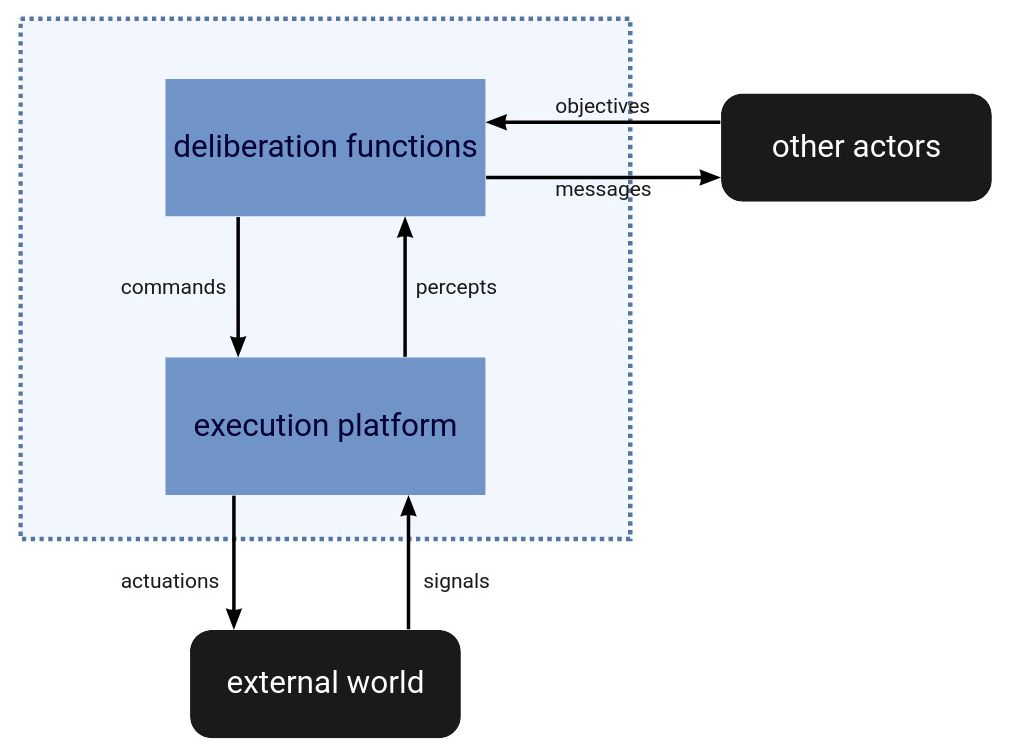
\includegraphics[width=\textwidth]{pics/GNT_actor_new.png}
        \caption{\textsc{Actor based on Ghallab et al. \cite{GNT:2016}}}
        \label{fig:GNT_actor}
    \end{subfigure}
    \hfill
    \begin{subfigure}[b]{0.49\textwidth}
        \centering
        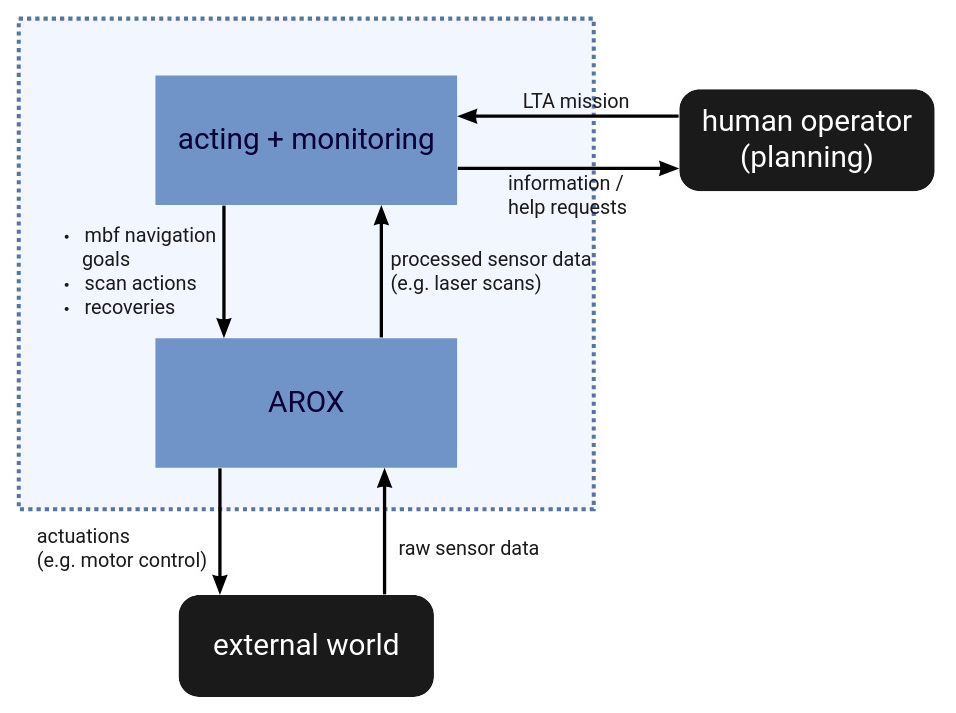
\includegraphics[width=\textwidth]{pics/MSC_actor_new.png}
        \caption{\textsc{Applied to our Scenario (cf. \ref{sec:prototype_scenario})}}
        \label{fig:MSC_actor}
    \end{subfigure}
\caption{\textsc{Abstract Architecture for Autonomous Actors}}
\label{fig:abstract_actor}
\end{figure}
\noindent
As anticipated before and visualized in fig. \ref{fig:abstract_actor}, the deliberation functions studied in this work are acting and monitoring. Furthermore, planning plays a role,
but is only relevant for retrieving and executing plans that are provided by a human operator, i.e. the human operator is essentially the planning component in our scenario.
Moreover, the human operator is the only other actor with whom the robot must interact. The communication between the robot and the operator will be discussed in detail later (cf.
\ref{sec:solutions_for_lta_challenges}), but the general idea is that it is a bidirectional channel that allows the operator to send LTA missions to the robot and, on the
other hand, allows the robot to transmit status information and help requests to the operator. Processed sensor data, mainly in the form of laser scans, is provided to the
acting and monitoring modules by the AROX execution platform presented in section \ref{sec:robotic_system}. Responsible for initiating the actual execution of low-level actions
are the deliberation functions that are also capable of sending commands such as \code{move_base_flex} navigation goals or recovery instructions to the AROX system.
Obviously, the AROX interacts with its environment via its sensors and actuators.\newline
Plan execution, as well as robot operation monitoring, i.e. the \textquote{deliberation functions}-module in fig. \ref{fig:abstract_actor}, is modeled as a high-level hierarchically
structured state machine, whose architecture is shown in figure \ref{fig:high_level_smach}. The capabilities of a certain degree of failure tolerance are commonly not a directly
integrated part of the control architecture, if considered at all. \cite{Khalastchi:2018} This is different in this thesis.
The architecture is implemented using the SMACH\footnote{ROS-independent Python
library to build hierarchical state machines \cite{smach}} library. The main objectives of monitoring are to detect deviations between what is expected and what is observed
(fault detection), diagnosis of the reasons for such deviations (identification), and provision of recovery options. \cite{Ingrand:2017}
If the behavior of a robotic system is plan-based, i.e., the operations of the robot are determined by some kind of plan, this is very meaningful for monitoring because the current
state of plan execution provides context and thus certain expectations. \cite{Khalastchi:2018} If, for instance, the robot is recording a scan in front of a plant, it may be useful
to start sensor monitoring, i.e. to check whether this operation results in a reasonable-looking scan that is successfully saved to disk.
\begin{figure}[H]
    \centering
    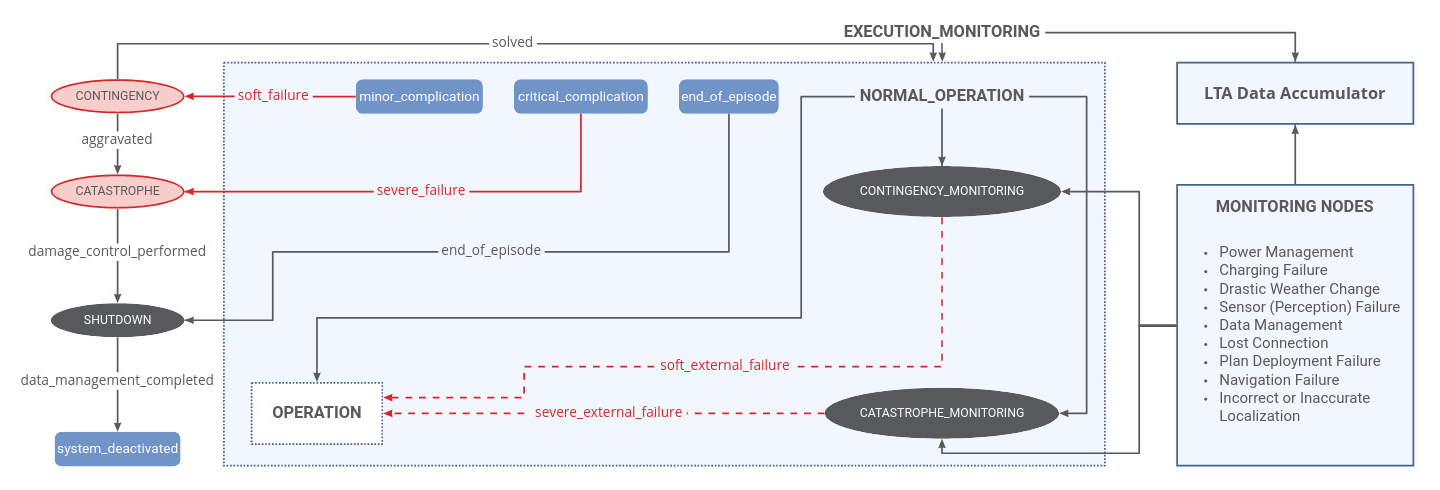
\includegraphics[width=\textwidth]{pics/SMACH_high_level.png}
    \caption{\textsc{Architecture of the Hierarchical State Machine (High-Level)}}
    \label{fig:high_level_smach}
\end{figure}
\noindent
As depicted in figure \ref{fig:high_level_smach}, the robot starts in the state \code{NORMAL_OPERATION} in the high-level hierarchical state machine \code{EXECUTION_MONITORING}.
\code{EXECUTION_MONITORING} coordinates the entire operation and is composed of the states \code{NORMAL_OPERATION}, \code{CONTINGENCY}, \code{CATASTROPHE}, and \code{SHUTDOWN}.
\code{CONTINGENCY} and \code{CATASTROPHE} essentially refer to type $(1)$ and type $(2)$ in fig. \ref{fig:problem_types}, respectively.
\code{NORMAL_OPERATION} is represented by an embedded state machine named \code{OPERATION}, visualized in figure \ref{fig:low_level_smach}, as well as the two
parallel running execution monitoring states (cf. ROS \code{MonitorState} \cite{monitor_state}) \code{CONTINGENCY_MONITORING} and \code{CATASTROPHE_MONITORING}, 
implemented as a concurrence container (cf. SMACH \code{Concurrence} \cite{concurrence_container}).
These parallel running states are used to monitor the robot's operation and to interrupt it when a problematic situation requiring special treatment is detected
(see the dashed arrows in figure \ref{fig:high_level_smach}).
When this case occurs, based on how severe the problem is, the respective procedure will interrupt \code{OPERATION} and provide for the outcome \code{critical_complication} or
\code{minor_complication}, which will then result in a state transition to the appropriate states in which the problem will be addressed. There is quite a bit behind
\code{CONTINGENCY}, namely the handling of the problem based on the problem type that is communicated along with the message of the interruption.
If \code{CONTINGENCY} is able to solve the problem, the \code{NORMAL_OPERATION} will resume (cf. top arrow). In case of \code{critical_complication} or if the robot was not able to
solve the problem, it ends up in the \code{CATASTROPHE} state, the human operator is notified, a backup is made if necessary, etc., and then the robot shuts down.
The interrupts of \code{OPERATION} are initiated by the monitoring nodes, which are shown on the right in fig. \ref{fig:high_level_smach}, and which detect problems as generally
as possible for each identified problem category.
Although a monitoring solution could in principle also be implemented sequentially, it seems more natural to choose a parallel approach, since a sequential option
would have the disadvantage that no monitoring takes place while a task / algorithm is being executed, but only afterwards.
It is desirable to be able to intervene at any time during the execution of a task when a monitoring procedure running in parallel is triggered and causes a change of state.
During the state \code{OPERATION}, i.e. in the nested state machine visualized in figure \ref{fig:low_level_smach}, the robot can be either in the state \code{IDLE}, 
in which it is waiting for a plan $\pi$, or in \code{EXECUTE_PLAN}, in which it is executing a given plan $\pi$. The embedded state machine \code{OPERATION} has 
four possible outcomes - \code{end_of_episode}, \code{minor_complication}, \code{critical_complication}, and \code{preempted}. 
It starts in the \code{IDLE} state and remains there as long as no plan $\pi$ is provided via a ROS service.
There are two common options for the robot to leave the state. The first is via a message on a ROS topic indicating that the end of the current long-term episode
has been reached, resulting in an overall outcome of \code{end_of_episode} for \code{NORMAL_OPERATION}. The second is to receive a plan $\pi$ that results in a state
transition to \code{EXECUTE_PLAN}. Additionally, the external parallel running monitoring states \code{CONTINGENCY_MONITORING} and \code{CATASTROPHE_MONITORING}
are capable of interrupting the \code{IDLE} state at any time (cf. state preemption \cite{state_preemption}) due to external problems leading to the outcome \code{preempted}.
In \code{EXECUTE_PLAN}, there are five possible outcomes, two of which result in state transitions and three of which cause \code{OPERATION} to return to the parent state machine.
The first possible outcome is \code{action_completed}, which indicates that an action $a \in \pi$  was completed successfully and causes the same state (\code{EXECUTE_PLAN}) to be
executed again with the reduced plan $\pi := \pi \backslash \{a\}$, i.e. the rest of the plan is executed. The next possible outcome is \code{plan_completed}, which means that the entire
plan $\pi$ has been successfully processed, i.e. $\pi = \emptyset$, and causes a transition back to the \code{IDLE} state.
These were the possible outcomes that cause a transition to another state. Now there are the three remaining outcomes that cause a return to the parent state machine. 
First, \code{soft_failure}, which means that something went wrong, e.g. an action $a \in \pi$ was not performed successfully, but the robot should be able to handle the problem. 
Second, there is the potential outcome \code{severe_failure}, which represents situations where the robot is unable to solve the problem itself.
Finally, the last potential outcome is again \code{preempted} based on some external issue detected by \code{CONTINGENCY_MONITORING} or \code{CATASTROPHE_MONITORING}.
In summary, there are two types of problems, low-level problems that are detected directly at this level, e.g. by simple error treatment, which then lead to an interruption based
on the severity of the problem, in this case \code{soft_failure} or \code{severe_failure}, which is then passed up to the high-level SMACH and handled accordingly.
The other, much more common case is that a problem is detected by the monitoring nodes. The consequence is that the execution is simply interrupted here and the problem is solved
at a higher level. Then \code{OPERATION} is restarted (cf. \code{external_problem} in fig. \ref{fig:low_level_smach}).
\begin{figure}[H]
    \centering
    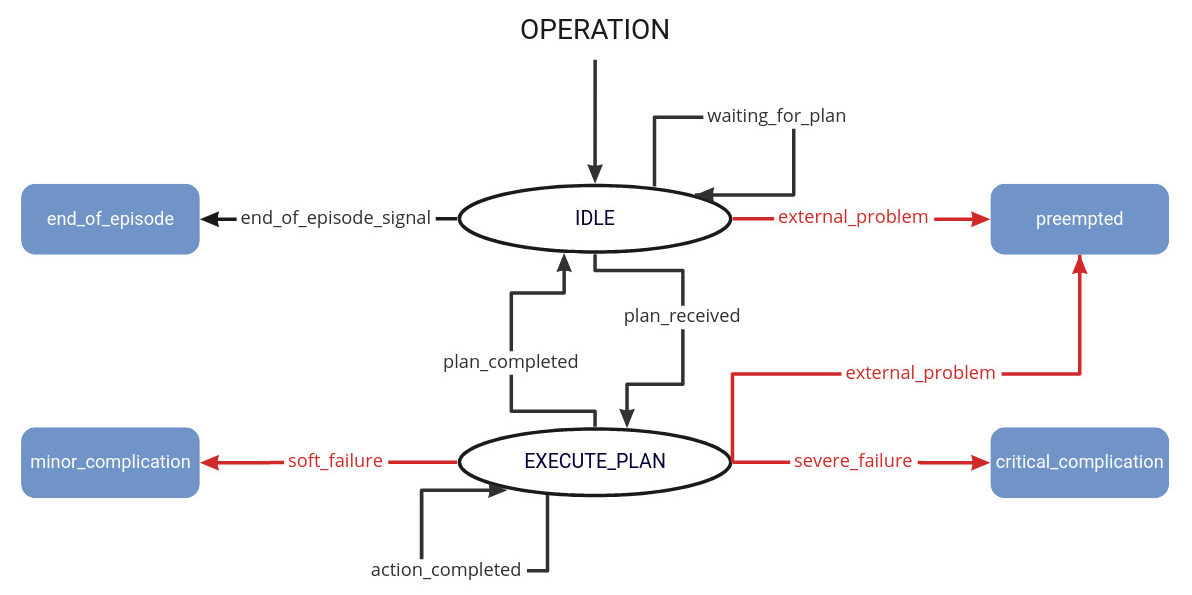
\includegraphics[width=0.8\textwidth]{pics/SMACH_low_level.png}
    \caption{\textsc{Architecture of the Embedded State Machine (Low-Level)}}
    \label{fig:low_level_smach}
\end{figure}
\noindent
Now that the control flow of \code{NORMAL_OPERATION} and, in particular, \code{OPERATION} has been clarified, we return to the parent state machine shown 
in figure \ref{fig:high_level_smach}.
As mentioned, when \code{NORMAL_OPERATION} returns \code{end_of_episode}, the parent state machine transitions to the \code{SHUTDOWN} state and the 
robot's work for that long-term episode is complete, which means that the robot performs data management and then the system is deactivated.
Essentially, in a long-term episode in the considered scenario, the robot should stay in \code{NORMAL_OPERATION} as 
long as the episode is running or an error / problem has occurred, either an error that it is able to deal with itself or even a more severe problem that requires the 
intervention of a human operator. Accordingly, if \code{NORMAL_OPERATION}, i.e. the embedded state machine together with the parallel running monitoring states has the outcome 
\code{minor_complication}, the robot enters the state \code{CONTINGENCY}, which means that it has detected a soft failure, e.g. a sensor failure, but its ability to act
is preserved, it is for example able to drive back to the base in safety mode. However, if \code{NORMAL_OPERATION} returns \code{critical_complication}, there is a severe 
failure that is unsolvable for the robot, perhaps even for the operator, and the robot transitions to \code{CATASTROPHE}. If it is still possible, the robot saves the current 
state of the plan execution, sends an emergency signal, e.g. communicates the problem to the operator, and shuts down, i.e. transitions to \code{SHUTDOWN}.
There are, of course, situations in which the robot can no longer do anything, such as when the battery is completely discharged.
In principle, such cases also fall under the category of catastrophe, but since monitoring then no longer works, there is nothing left to do there.
Besides, there are two more transitions depicted in figure \ref{fig:high_level_smach}: From \code{CONTINGENCY} back to \code{NORMAL_OPERATION}, after a minor problem is resolved by the robot, it can continue
its normal operation. Additionally, it is possible that something goes wrong during \code{CONTINGENCY} or that the problem actually cannot be solved by the robot,
such that it transitions to \code{CATASTROPHE}.\newline
To be clear, \code{NORMAL_OPERATION} can manage problems in two ways.
First, a problem may occur during plan execution in the child state machine, in such a case \code{OPERATION} returns \code{critical_complication} or 
\code{minor_complication} to the parent state machine based on the problem severity and a corresponding state transition takes place.
In addition, there are the described parallel monitoring states, which are responsible for problems that are not directly related to plan execution, but are of a more general nature.
If these detect a problem, they are able to interrupt \code{OPERATION} and also return \code{critical_complication} or \code{minor_complication} to the parent state machine
\code{EXECUTION_MONITORING}. It is trivial to interrupt \code{OPERATION} when no task is currently being executed, i.e. no scan is being recorded and no navigation target 
is being approached. However, it is obvious that potential problems do not wait for the completion of such tasks, but can also occur during the execution of an action $a \in \pi$.
Therefore, the \code{drive_to(lat, lng, theta)} and \code{scan} actions are implemented as ROS \code{SimpleActionClient}s that can be interrupted at any time
by calling the \code{cancel_all_goals()} method, which immediately interrupts all running goals. It is quite important that the robot is able to preempt the plan 
execution at all times, e.g. does not continue to drive to its goal, but should instantly stop the \code{move_base_flex} goal execution and start following the
recovery instructions.\newline
The general difference between the \code{CONTINGENCY} and \code{CATASTROPHE} states is the robot's ability to act. 
In a catastrophe case, it is no longer really capable of acting in the sense of driving back to its base, managing the problem itself, etc. 
An example for a catastrophic case would be that the robot falls over. It is then unable to recover, but it is of course still able to communicate the problem
and save the state, in full possession of its ``mental'' powers, so to speak. Whereas a lightning strike, as an extreme example, could cause the robot to have a 
complete breakdown and nothing to work at all. The boundaries there are not quite sharp, there are many edge cases.
The following somewhat more mundane example, considering the robot's battery, will illustrate the concepts.
In \code{NORMAL_OPERATION} the battery does not discharge precisely according to the plan. There may be some fluctuations due to temperature, for example.
The power management monitoring node would initiate a transition to the state \code{CONTINGENCY} when it detects that the battery is already too low to complete the plan until the
next charge stop, but it is still able to recover, i.e. drive back to its base, recharge, and continue the plan execution. However, it would proceed to \code{CATASTROPHE} if it
detects that the battery is so low that it can already tell that it is not possible to reach the base and recharge. It is then still able to communicate the problem and save the
state, but it is definitely not able to recover. This leads to a message to \code{CATASTROPHE_MONITORING}, then to an external failure, which interrupts \code{OPERATION} with a
\code{critical_complication} and causes the high-level state machine to transition to \code{CATASTROPHE}. The problem is communicated and the robot shuts down. The extreme case,
where nothing can be done, would be that the battery suddenly just breaks. Finally, there is also the case that first a \code{CONTINGENCY} is launched as the problem still seems to be
solvable based on current estimations and then it turns out that it in fact is not. For instance, when the discharge rate is furthermore increased. In such a case, it turns out during
the solution that it does not work anymore, i.e. the assumption was wrong, it is no longer solvable, then it comes to the \textquote{aggravated} case, i.e. the problem worsens and then
becomes a \code{CATASTROPHE}. Additionally shown in fig. \ref{fig:high_level_smach} is the data accumulator that logs all relevant information from the execution and monitoring nodes.
On the one hand for debugging purposes, but also to be able to learn from it later on, which will be discussed in section \ref{sec:black_box}.

\section{Black Box to Learn from Experience}
\label{sec:black_box}

From a software engineering perspective, it makes sense to create an interface for machine learning or general analysis in the architecture, even if it is not yet explicitly used.
This interface is intended for a concrete configuration, e.g. the AROX system with its sensors (cf. section \ref{sec:robotic_system}), the rationale being to learn from experience. The robot operates in an environment for an
extended period of time. Therefore, it is very valuable to collect data about the robot, its interaction with the environment, faults, etc. through extensive logging, with special
emphasis on fault context. Whenever something goes wrong, it is interesting to learn the reason for this problem. For a specific sensor setup, one could use learning techniques or
statistical methods in general to infer that a particular effect occurs experientially. For instance, experience might show that a particular sensor failure occurs repeatedly when driving $> 4$ hours at
$> 32$\textdegree{}C. A further example could be that the robot always has a failure after passing a certain waypoint. To determine this, it would be necessary to always
log the current location of the robot along with a problematic situation. This list could be arbitrarily extended.
In general, the objective is to avoid certain behaviors that have frequently led to failures in the past. Information about such effects can only be
obtained through runtime experience, which shows how relevant such information are and how crucial it is to collect them. So gathering information should go along with long-term
operation. The actual learning of such effects is beyond the scope of this thesis. Yet, the creation of an appropriate interface in the architecture and the collection of information
are part of the developed framework. The idea of gathering information and learning from it is natural, because that is essentially what a human operator would do as well, gaining
experience and improving over time. Essentially, in a problematic situation, it is a matter of logging what the associated relevant circumstances are. Of course, this would just be
the output of the system and the input to some sort of learning or analysis software. Nonetheless, if some regularities have been learned or identified from the logged data, they can
be exploited and it should be possible to feed that information back to the system, i.e., the path in the other direction. Unfortunately, since this is usually information of the type
\textit{in the event of $X$, do $Y$}, it is not trivial to feed it back automatically and actually apply it in a meaningful way. It would be possible to report back messages that
indicate problems based on learned regularities, but it is not as simple to create a way to automatically generate an appropriate response from the robot to avoid the problem. There
can be an arbitrary number of possible actions that are required, and the only truly viable solution is to provide a general and easily extensible framework so that learned
regularities can be implemented as advanced monitoring and resolution methods. Now, one could argue that such a feedback option would still be valuable for the learned messages that
indicate problems. However, this does not help significantly, as these messages have already been logged in erroneous situations, which have thus inevitably already been detected by
the existing monitoring solutions. The broad idea of learning from experience in long-term autonomous operation is not new, of course, and some examples have already been given in the
literature review in section \ref{sec:literature_review}. Hawes et al. \cite{Hawes:2017} also emphasize the usefulness of the information gathered in long-term autonomous operation for both learning and troubleshooting
purposes. For information gathering, they use \code{mongodb_store}\footnote{https://wiki.ros.org/mongodb\_store}, a ROS tool for storing data from a ROS system (messages,
configurations, etc.) in a \textit{MongoDB} instance, i.e., a document-oriented database. To achieve systematic and reusable logging and general data acquisition, this tool is also
used in this thesis. For this purpose, a \code{data_accumulator} node was written to capture the relevant data during LTA missions and store it in the database. Initially, a
\code{MessageStoreProxy} object is created to enable updating and maintenance of the \textit{MongoDB} database. Various logging categories are defined to semantically group the
collected data. Each component of the monitoring framework, i.e. each node, can initiate logging to the database under a specific category based on ROS topics provided by the
\code{data_accumulator}. To store an entry under a category or name, the \code{insert_named("name", entry)} method of the \code{MessageStoreProxy} is used. It is obviously relevant
to log contingency and catastrophe situations, which is why \code{/contingency_preemption} and \code{/catastrophe_preemption} lead directly to a database entry under the categories
\code{contingency} and \code{catastrophe} respectively. The content of this entry is in each case the message describing the problem that occurred. Whenever a contingency or
catastrophe situation is logged, the node triggers a method \code{log_failure_circumstances()} because, as mentioned earlier, the particular circumstances of a problematic
situation, i.e., the potential factors leading to the problem, can be very revealing. For the moment, the specific additional contextual information comprises, in addition to the
information logged anyway, the position of the robot in longitude and latitude obtained from \code{/fix}, as well as the number of tasks completed, the current operating time,
the charge level and the current charge cycle. This
list can be extended in the future as needed. All this information is stored summarized in a JSON dump under the category \code{failure_circumstances}. Numerous insightful but less
critical information about the robot and its environment is logged under the category \code{robot_info}, received as messages on a topic with the same name. In simulated experiments,
it is also critical to know exactly when error situations have been simulated. Therefore, all nodes simulating problem situations can report under the \code{/sim_info} topic when they
do so, and the messages are stored under the same category in the database. The \code{/action_info} topic is responsible for the also very relevant information about the currently
executed action, which is stored under the name \code{action_info}. Moreover, there are \code{/operator_communication} and \code{/resolution} that store any logged message between
the operator and the robot as well as any executed resolution methods under the same names. It is furthermore important to keep track of missions, which is why new messages via
\code{arox/ongoing_operation} are also logged. Finally, for debugging purposes, there is a \code{/show_db_entries} topic that allows to list
all database entries for the current LTA mission or the entries under a particular category specified by the string message published to the topic. The path for the
database can be configured in the launch file. Once a \textit{MongoDB} server is running with the generated database, ie. \code{mongod --dbpath ROS_db --storageEngine=wiredTiger},
a \textit{MongoDB} client can connect and examine the logged data. It can be visualized and queried in JSON, for example, as shown in fig. \ref{fig:database_entries}.
This shows, for instance, a contingency due to a failed docking attempt. This is immediately followed by the explicit error conditions, e.g. state of charge, tasks completed, charge
cycle, position and operating time. Besides, many aspects that are logged at the same time under \code{robot_info} are not displayed here. Subsequently, the resolution follows, the
charging failure resolver is started together with the information describing the problem.
\begin{figure}[H]
    \centering
    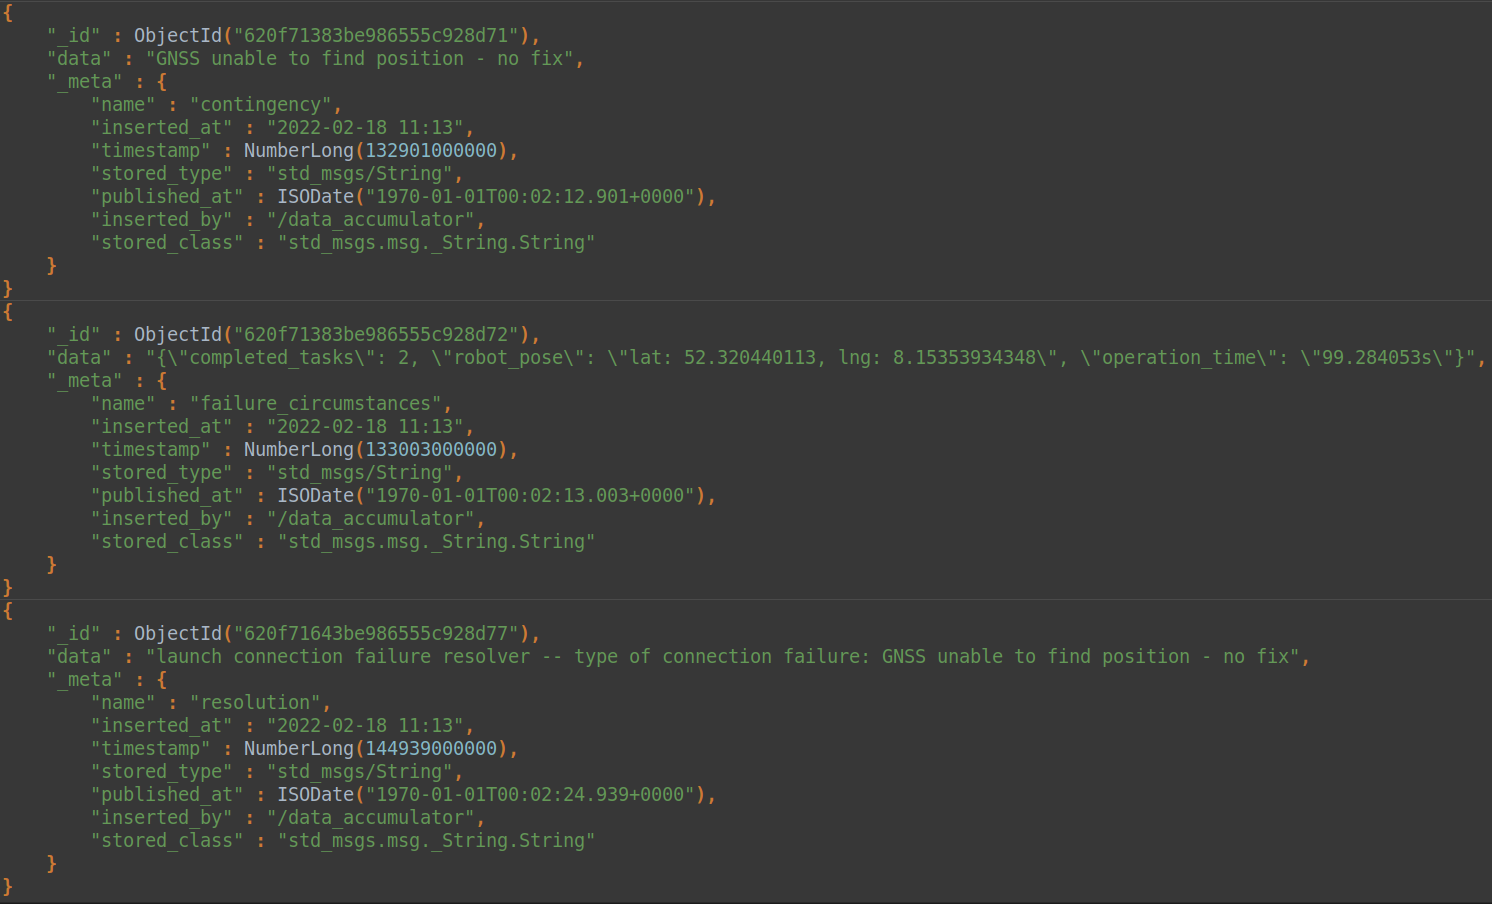
\includegraphics[width=\textwidth]{pics/database_entries.png}
    \caption{\textsc{Database Entries Shown in} \textit{MongoDB} \textsc{Client}}
    \label{fig:database_entries}
\end{figure}

\section{Interruption and Resumption of Normal Operation}
\label{sec:plan_interruption_section}

\textquote{\textit{Plans must be executed according to some strategy. This must account for action failure, plan failure due to ignorance or change in a dynamic environment [...].}}
\cite{Cashmore:2015}
In order to handle unexpected problematic situations, the robot must be able to stop and resume its normal operation in general
and plan execution in particular, i.e. to save the current state of the plan execution and resume exactly that state after the reason
for the interruption has been resolved. The idea is that whenever the monitoring procedures \code{CONTINGENCY_MONITORING} and \code{CATASTROPHE_MONITORING} 
introduced in section \ref{sec:execution_monitoring_smach_architecture}, or the plan execution itself, detect a problem, they should trigger such an interruption.
As seen in section \ref{sec:execution_monitoring_smach_architecture}, there are two states in \code{OPERATION} that the robot can be in during a long-term episode without any problems
- \code{IDLE} or \code{EXECUTE_PLAN}. In the \code{IDLE} state, where it waits for the plan generator described in section \ref{sec:plan_generation} to provide a plan $\pi$,
it is straightforward, the normal operation is interrupted, the high-level state machine transitions to \code{CONTINGENCY} or \code{CATASTROPHE} depending
on the severity of the problem, and then, i.e. when the minor problem is resolved, it transitions back to \code{IDLE} or, in the case of \code{CATASTROPHE},
it shuts down. The more interesting case, of course, is such an interruption of normal operation when the robot is in the low-level state \code{EXECUTE_PLAN}.
In this case, a plan execution must be interrupted.
During the \code{EXECUTE_PLAN} state, the currently executed plan $\pi$ is always stored in the \code{userdata} field of the state.
SMACH states always provide so-called \code{userdata} fields, which are essentially the input and output data of a SMACH state.
Initially, when \code{IDLE} receives a plan $\pi$ from the plan generator, it passes it as \code{userdata} to the \code{EXECUTE_PLAN} state. Then, whenever \code{EXECUTE_PLAN}
successfully completes an action $a \in \pi$, the reduced plan, i.e. $\pi := \pi \backslash \{a\}$, is passed to the next iteration of the same state.
Therefore, based on this architecture, the current state of the plan execution is always stored in the \code{userdata} of the SMACH. To comply with this fact, a certain situation
must be handled. If a plan execution is interrupted during the execution of an action $a \in \pi$, the action $a$ is already removed from the plan $\pi$, i.e. the \code{userdata},
by the latest \textit{pop} operation and since the execution of $a$ must be repeated when the normal operation resumes, $a$ must be reattached to $\pi$ before transitioning
to \code{CONTINGENCY} or \code{CATASTROPHE}. Thus, $\pi := a.\pi$.
Of course, when the robot transitions back to \code{NORMAL_OPERATION} after solving a contingency, it starts again in \code{IDLE}, which is why \code{IDLE}
always looks for existing unfinished plans $\pi$ in the \code{userdata} first. If there is one, i.e. $\pi \in$ \code{userdate.input_plan}, $\pi \neq \emptyset$, it does not prompt the
plan generator for a new plan, but continues the previously preempted and only partially completed plan $\pi$.
The catastrophe case works analogously to the \code{IDLE} state.\newline
Of course, it is not necessarily always feasible to simply execute the rest of the plan afterwards, since the planned charge stops may no longer be sufficient. However, if the
interruption of the plan involves returning to the base and seeking shelter, this is not a problem, since such a recovery can always be accompanied by recharging, so that the
battery is fully charged when the robot resumes its operation. In such a case, it might even be feasible to remove some of the next planned charge stops. If a charge stop is one
of the actions immediately following, this simple plan modification is performed. Nevertheless, there are cases in which the robot does not return to the base and has to consume
unplanned resources, so that the a priori planned charge stops are rendered insufficient. This problem, though, is addressed by the integrated battery monitoring module described
in section \ref{sec:battery_monitoring}, which detects this and initiates a return to base. In conclusion, the continuation of plan execution works either way.

\section{Simulation and Monitoring of LTA Challenges}
\label{sec:sim_and_mon_of_lta_challenges}

Now that the overall architecture of the execution monitoring state machine has been described (cf. section \ref{sec:execution_monitoring_smach_architecture}), we can turn to the
actual monitoring methods for the potential hinderances for long-term autonomous systems introduced in section \ref{sec:challenges_for_lta}. The idea is to implement a specific
monitoring procedure for each of the selected LTA problems that runs in parallel to the high-level state machine. Whenever such a procedure is triggered, i.e. the specific issue
is recognized, the problem gets reported via the \code{MonitorState}s, causing a transition to \code{CONTINGENCY} or \code{CATASTROPHE} based on the severity of the problem.
Depending on the nature of the problem, the information about the required solution method is conveyed via the message published to the topic of the \code{MonitorState}.
Thus, the long-term goal is to have a resolver node for each of the potential failures, which is executed in \code{CONTINGENCY} or \code{CATASTROPHE} depending on the
failure case at hand. It is useful to distinguish between internal and external exceptional situations that require special treatment, i.e. issues concerning the robotic
system itself or the environmental conditions. \cite{Hawes:2017}
The entire process is essentially the same for all potential LTA problems - fault simulation, monitoring, and subsequent remediation. Initially, it will be demonstrated that in the
prototypical scenario, the mission can no longer be completed successfully if these errors occur (cf. section \ref{sec:experiments}). After launching the monitoring nodes, the
problems should be detected and either resolved by the robot or reported to the operator so that the mission can continue. All of the simulated failures are implemented in a way that
allows them to be triggered by publishing to a certain topic in order to enable automation of these failure cases in subsequent experiments (cf. section \ref{sec:experiments}).
In the following, the simulation of the selected LTA problems is presented along with the monitoring solutions developed for each.

\subsection{Power Management}
\label{sec:sim_and_mon_power_management}

Power management issues are addressed based on the integrated battery watchdog module described in section \ref{sec:battery_monitoring}, which monitors the state of the battery
and acts as a fail-safe. The integrated watchdog module constantly publishes one of three states on the topic \code{/watchdog}. \code{"NORM"} indicates that the energy consumption is
as expected and no problem has been detected. In contrast, \code{"CONT"} and \code{"CATO"} represent situations in which the a priori planned charge stops are no longer feasible. In the
event of a contingency, i.e. \code{"CONT"}, an immediate return to the base station is required in order to still be able to reach it. Even more severe, in a catastrophe situation, ie.
\code{"CATO"}, it is no longer possible to reach the base station due to the battery charge level. The monitoring node simply subscribes to the \code{/watchdog} topic and initiates
appropriate responses based on the signals sent by the battery watchdog module. In case of a \code{"CONT"} message, \code{/contingency_preemption} is used to initiate a contingency
and communicate the specific reason. Likewise, in case of \code{"CATO"}, a catastrophe is triggered with \code{/catastrophe_preemption}. The node distinguishes between catastrophe
and contingency monitoring, since a contingency can be followed by a catastrophe situation. Thus, when a contingency occurs, active monitoring is suspended for \code{"CONT"} messages,
but the node continues to check for \code{"CATO"}. In fact, it is quite natural for a contingency to precede a catastrophe, since it is rather rare for the battery to suddenly drop in
such a way as to eliminate the possibility of returning to base. Therefore, catastrophe events should be able to interrupt contingencies, so monitoring must remain active during
contingencies. Monitoring for both is re-enabled when the robot is fully charged, indicated by a message on \code{/fully_charged}. For the power management monitoring node to be
applicable, a system must either incorporate the integrated battery watchdog module presented in section \ref{sec:battery_monitoring} or provide a similar module that publishes the
three expected states on the \code{/watchdog} topic. Additionally, a fully charged battery is expected to be communicated via the \code{/fully_charged} topic.\newline

\noindent
Power management problems can be simulated quite easily based on a controllable battery consumption model that can be manipulated at will. Both cases are simulated by creating a
\code{dynamic_reconfigure}\footnote{https://wiki.ros.org/dynamic\_reconfigure} client and manipulating the discharge rate of the robot's battery. Depending on the simulation case, i.e. contingency or catastrophe, different
user-configurable discharge rates are set. After the expected event is triggered, the discharge rate is reset to the default value. This is particularly relevant for contingency
cases, as otherwise a catastrophe would often follow due to the increased discharge rate. Power management failure simulation can be enabled using the following ROS topics:
\begin{itemize}
    \item \textbf{contingency} \textrightarrow \code{/sim_power_management_contingency}
    \item \textbf{catastrophe} \textrightarrow \code{/sim_power_management_catastrophe}
\end{itemize}
Power management failures can be addressed with the resolution methods described in section \ref{sec:power_management_resolver}.

\subsection{Charging Failure}
\label{sec:sim_and_mon_charging_failures}

As anticipated in section \ref{sec:challenges_for_lta}, (un-)docking to the charging station may fail or the charging process itself may not start after docking. Both cases should be
detected by the robot so that an appropriate response can be initiated, e.g. notification of the human operator. Thus, charging failures are not only considered explicitly, but also
as situations that imply charging failure (failed docking) or prevent successful continuation of the mission after charging (failed undocking). In general, the following remarks on docking,
undocking, and charging refer to the integrated base station and charging infrastructure as well as the state machines for docking and undocking presented in section
\ref{sec:docking_solution}. Initially, it should be pointed out again that the failure cases identified in this thesis are not always strictly separated from each other. For instance,
based on their nature, (un-)docking errors could sometimes already be covered by navigation error monitoring, e.g. in the event of a sustained recovery (cf. section \ref{sec:sim_and_mon_navigation_failures}).
However, this does not cover all types of docking and undocking problems. The first type of docking error is an explicit error returned by the docking state machine and can be caused
by various problems, such as not being able to detect the container in the laser scan of the robot's surroundings. Likewise, explicit errors can be communicated by the undocking state
machine, which is started after the charging process is complete. To notify the monitoring procedure of such errors, the operation state machine, which catches them as part of general
error treatment, publishes them on the topic \code{/explicit_charging_failure} to which the monitoring procedure is subscribed. In this case, the monitoring node triggers a
contingency via \code{/contingency_preemption} and communicates the reason for the problem. Finally, there is the case that the charging process does not start after successful
docking, i.e. the battery charge does not increase. A failed charging process can be detected based on a specific time in the state of charge without increasing the charge level
of the battery. Specifically, the current state of charge is constantly tracked via \code{/arox/battery_param}, on which messages of type \code{arox_battery_params.msg} appear,
containing the fields \code{std_msgs/header header}, \code{float64 charge}, \code{int64 charging_cycle}, \code{string battery_operation}, \code{float64 operation_time}, and
\code{int8 env_condition}. In case a charge action is performed, which is communicated by the operation state machine via \code{/charge_action}, the current charge level is stored,
the procedure sleeps for a user-specified time and afterwards compares the current charging state with the previously stored one. If the most recent state of charge is not higher
than the one stored at the start of charging, a contingency is initiated because the battery is not charging despite the robot being docked to the charging station. For a system to
use the charging failure monitoring node, it must either use the docking solution described in section \ref{sec:docking_solution} for explicit docking failures, or, if it uses a
different docking solution, communicate its explicit docking failures via \code{/explicit_charging_failure}. Moreover, to use actual charge monitoring, it must employ the battery
watchdog described in section \ref{sec:battery_monitoring} or publish its own system's data in the expected format, i.e. as \code{arox_battery_params.msg}. The naming scheme, which
includes references to the AROX system, is somewhat misleading given the idea of a certain universality, but is retained at this point to remain compatible with the battery watchdog
module.\newline

\noindent
The identified failure modes can be simulated using the following approaches. Docking errors can be easily simulated by having the robot move to an inappropriate location before
docking so that it cannot detect the container because it is not in its environment. For this purpose, the user-configurable location to which the robot supposed to move when
executing an action \code{return_to_base} is exchanged with an inappropriate destination. The idea of this location is generally that it is roughly in front of the base station so
that it can be detected in a laser scan. Thus, the substitute position will be a completely different one, meaning that the detection of the container will inevitably fail.
This exemplifies cases where the detection part of docking fails. An example that causes the navigation portion of the docking process to fail would be raising the ramp of the
container so that there is no way for the robot to enter after successful detection. To achieve this, the joint position $j \in \mathbb{R}$ of the entry ramp of the container must be adjusted
accordingly by publishing a suitable value in radians to \code{/container/ramp_position_controller/command}. Figure \ref{fig:joint_positions} depicts the feasible joint position
range $j \in [0, \frac{\pi}{2}]$ of the container ramp. Accordingly, to fully raise the ramp and thus close the container, a value of $j = 0$ must be published.
\begin{figure}[H]
    \centering
    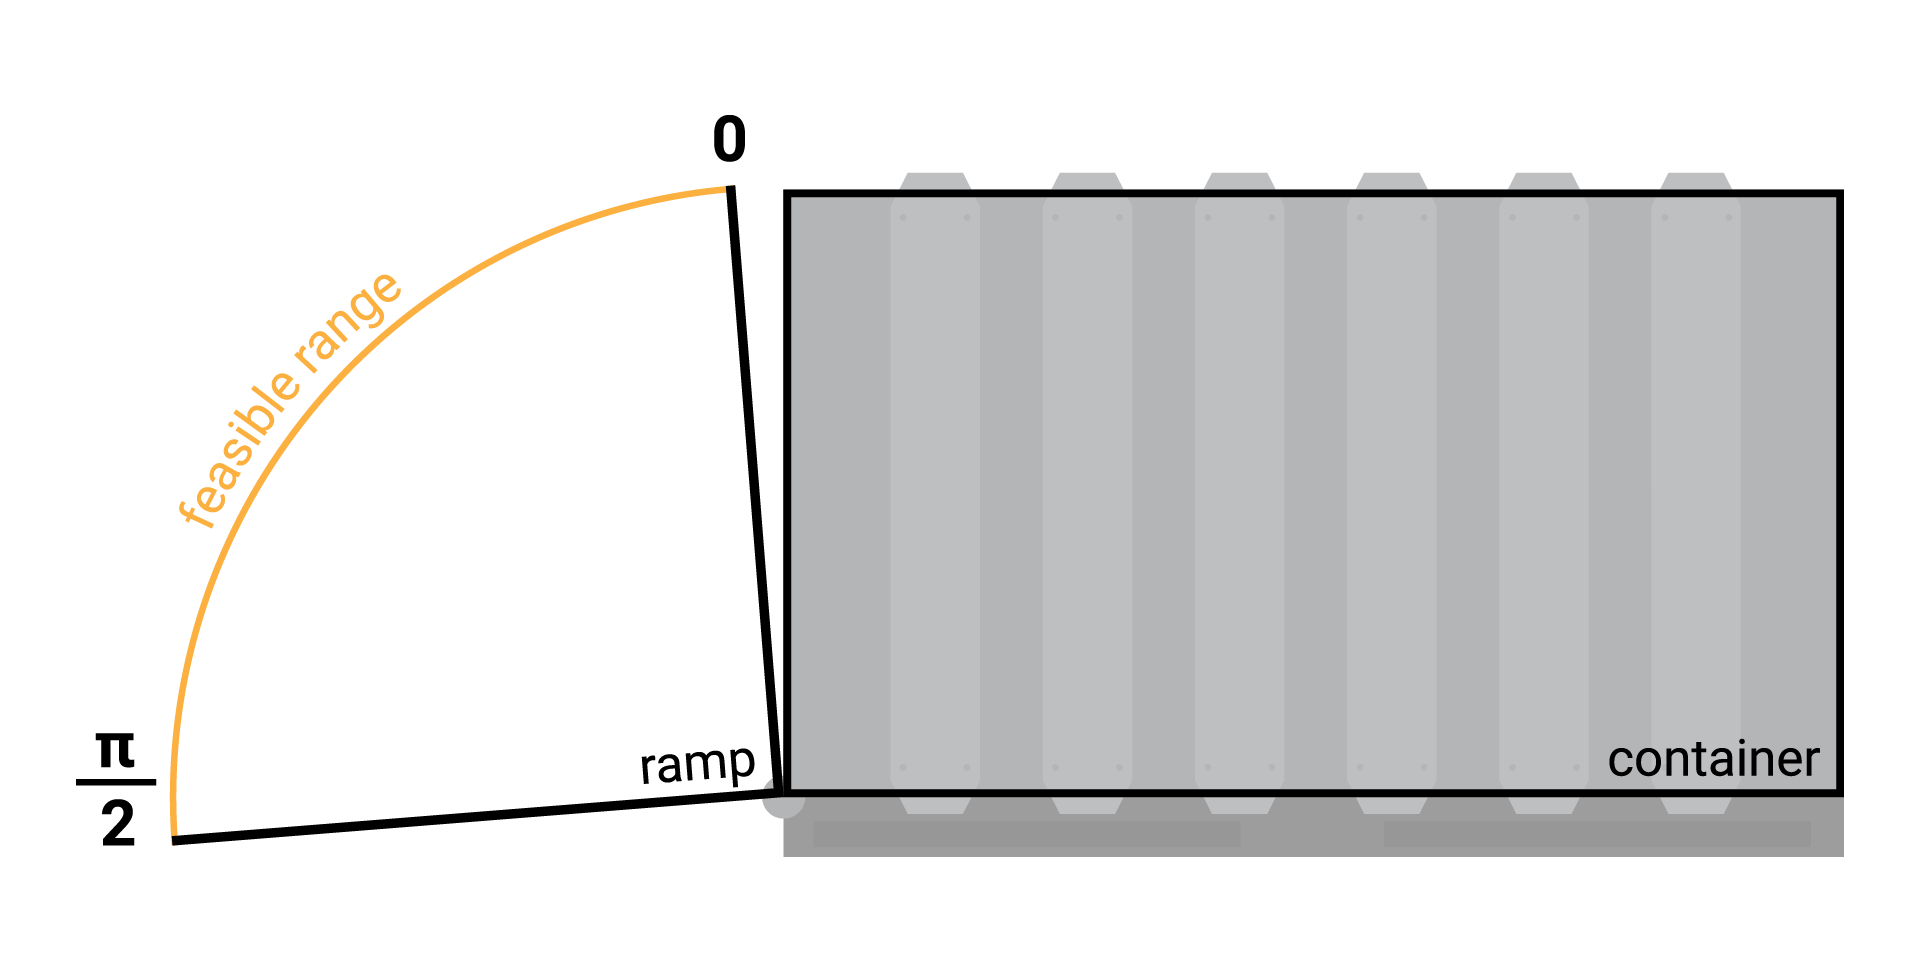
\includegraphics[width=0.6\textwidth]{pics/joint_position_container.png}
    \caption{\textsc{TODO: Entry Ramp Joint Positions}}
    \label{fig:joint_positions}
\end{figure}
\noindent
A closed container case could in principle also be detected by the navigation monitoring solution described in section \ref{sec:sim_and_mon_navigation_failures}, but such situations
are also recognized by the docking state machine, which returns an error after several entry attempts. Therefore, it is not determined which monitoring procedure is triggered first,
as this depends on the situation and environment, but generally one of the two nodes will be triggered and initiate resolution. Undocking errors are in principle not very diverse,
since it is only a question of leaving the container. They can therefore be simulated simply by a raised ramp, so that the robot is locked in the container. This is in turn achieved
by publishing $j = 0$ to \code{/container/ramp_position_controller/command} while the robot is inside the container. To ensure that the robot is actually inside the container when
this case is simulated, the execution of the simulation does not follow immediately after initiation, but waits until the next \code{charge} action indicated by the operation
state machine is executed. A noteworthy aspect of this simulation is that the robot cannot solve the problem itself, just as in the \textquote{robot prison} scenario in section
\ref{sec:sim_and_mon_navigation_failures}. Ultimately, a failed charge is also quite trivial to simulate based on a controllable battery consumption and recharge model.
Charge failure simulation can be enabled using the following ROS topics:
\begin{itemize}
    \item \textbf{undocking failure (raised ramp)} \textrightarrow \code{/sim_undocking_failure}
    \item \textbf{docking failure (raised ramp)} \textrightarrow \code{/sim_docking_failure_raised_ramp}
    \item \textbf{docking failure (wrong base pose)} \textrightarrow \code{/sim_docking_failure_base_pose}
    \item \textbf{charging failure} \textrightarrow \code{/sim_charging_failure}
\end{itemize}
Charging failures can be addressed with the resolution methods described in section \ref{sec:charging_failure_resolver}.

\subsection{Drastic Weather Change}
\label{sec:sim_and_mon_drastic_weather}

There are two ways to incorporate weather information, either by having the robot detect it with its own sensors or by utilizing external weather information. In any case,
it would be good to identify extreme weather conditions that could affect the proper functioning of the system in order to react accordingly, i.e. return to the base station and
seek shelter. Since we live in a world where local weather information is quite readily available and the robot's sensing capabilities would also be limited in its ability to
reasonably detect it, external weather information is used. In addition, realistic simulation of weather phenomena is a difficult task that would shift the focus of the work.
Thus, the robot does not detect extreme weather conditions itself through its sensors, but relies on external local weather data. To retrieve local weather information, a Python
wrapper of the \textit{OpenWeatherMap} API\footnote{https://openweathermap.org/api} is used, guaranteeing cross-platform applicability. Initially, the weather monitoring node
establishes a connection to the \textit{OpenWeatherMap} API. If successful, it continuously requests local weather data at a user-configurable frequency, e.g. every half hour.
As weather data should be based on the current location of the robot, the node maintains a subscription to the \code{/fix} topic described in section
\ref{sec:sim_and_mon_gnss_connection_problems}, through which \code{NavSatFix} messages containing the latitude and longitude of the robot's current presumed position arrive as
new GNSS data is made available. These coordinates are used to retrieve local weather information from the \textit{OpenWeatherMap} API. After parsing the data relevant for
monitoring, the actual monitoring at the user-specified frequency begins. First, the current rain volume $r_v$ in $mm/h$ is monitored based on two cases: If $7.6 > r_v > 2.6$,
the rain is considered moderate and manageable, so an information is published to the operator, but the robot continues its work. When $r_v > 7.6$, the rain is considered heavy,
causing the robot to interrupt its mission and launch a contingency. This classification of precipitation intensity stems from the American Meteorological Society's
\textit{Glossary of Meteorology}\footnote{https://glossary.ametsoc.org/wiki/Rain}. Analogously, the current snow volume $s_v$ is monitored in $mm/h$. When $2.0 > s_v > 0.5$, it is
considered bearable and only the operator is informed about the situation, but if $s_v > 2.0$, an interruption of the work is initiated. The next aspect monitored is the wind speed,
where \textit{OpenWeatherMap} distinguishes between a general wind speed and a gust speed. The former refers to a prolonged wind speed and the latter to sudden gusts of wind.
Since both can be dangerous for the operation of the robot, they are monitored together and summarized as wind speed $w_s$ in $m/s$ in the following. If $14.0 > w_s > 11.0$, the
robot continues its work but informs the operator of a \textquote{strong breeze}. When $20.0 > w_s > 14.0$, the robot still continues its work, but informs the operator of a gale
and that it is starting to get critical. When $28.0 > w_s > 21.0$, the robot interrupts its mission and informs the operator of a strong gale and the risk of structural damage.
Moreover, at $33.0 > w_s > 28.0$, the robot reports a storm force and a very high risk of structural damage and aborts its mission. Finally, at $w_s > 33.0$, it aborts its operations
and reports a hurricane and a very high risk of severe and extensive structural damage. Wind speed classification limits are based on wind speed estimates from the US Department of
Commerce's \textit{National Weather Service}\footnote{https://www.weather.gov/pqr/wind}. Furthermore, the temperature is monitored in \textdegree{}C based on $t_{min}$ and $t_{max}$,
the minimum and maximum temperatures measured in the robot's further surroundings, as well as $t$, the current temperature at the robot's location. It is reasonable to assume both
an upper and a lower limit for the temperature in the robot's working environment. As such lower and upper bounds depend heavily on the robotic system in question as well as its
sensor equipment, the limits are user-configurable. By default, a contingency due to excessive temperatures is initiated when $t > 40$ or $t_{max} > 40$. Likewise, the robot
interrupts its mission due to extreme cold when $t < -5$ or $t_{min} < -5$, e.g. because this could be problematic for the system's battery. The \textit{OpenWeatherMap} API
additionally provides a weather condition code\footnote{https://openweathermap.org/weather-conditions} for each situation, which is well-suited for systematic monitoring.
Based on these codes, it is easy to interrupt the mission for all possible variants of thunderstorms. Besides the specific checks for precipitation amounts mentioned above,
there are also codes for variations of heavy rain and snow that are used as indicator for contingencies. Additionally, codes for squalls, tornados, and atmospheric features
such as mist, smoke, or fog are used to interrupt the mission. Eventually, the \textit{OpenWeatherMap} information also contains the sunrise and sunset times. Since the robot
requires daylight for its missions, it also interrupts them when it approaches or even exceeds sunset or when it tries to start before sunrise. Of course, all upper and lower bounds
for the attributes of the current weather situation are in principle configurable by the user, but are set to reasonable default values from the literature.  In all contingency
cases, the weather monitoring node publishes a message on the \code{/contingency_preemption} topic indicating the particular type of weather condition and causing a transition to
the \code{CONTINGENCY} state where an appropriate resolution method is selected and launched. Afterwards, it transitions to a kind of passive monitoring mode where it no longer
triggers contingencies etc., but only waits until the weather situation is moderate again and reports this on the topic \code{/moderate_weather}. In addition, it listens to a
topic where the resolver provides its results. If successful, the weather monitoring transitions to active monitoring again.
Similarly, the information that does not require interruption of the mission is transmitted via the \code{/robot_info} topic. Aside from the
information relevant to monitoring, there is some other information that may be of interest to the operator. Therefore, a full weather report can be configured to be communicated
to the operator at specified intervals, e.g. once a day. Beyond those already discussed, this information includes observation time, a general status description, the cloudiness
percentage, the humidity, the atmospheric pressure and the wind direction. In order for a system to utilize the weather monitoring node, it should provide \code{NavSatFix} data on
the \code{/fix} topic, as the weather information is based on the current location of the robot. Alternatively, the values for latitude and longitude can be configured explicitly.
Furthermore, an internet connection is required to connect to the \textit{OpenWeatherMap} API.\newline

\noindent
As always, in order to evaluate the monitoring procedures, a simulation of the various scenarios must be provided. This simulation takes place in the parser for
\textit{OpenWeatherMap} data. Based on the developed weather monitoring node, it is failry trivial to simulate the occurrence of such extreme weather conditions by simply setting
the attributes to extreme values, e.g. a heavy rain scenario can be simulated by setting the corresponding rain volume $r_v = 8$. Likewise, a heavy snow situation can be simulated
by setting $s_v = 3$. The simulation of the remaining extreme weather events can be triggered analogously. Weather-related challenges for LTA can be dealt with using the resolver
described in section \ref{sec:weather_resolver}. Simulating extreme weather events can be activated / deactivated via the following ROS topics:
\begin{itemize}
    \item \textbf{heavy rain} \textrightarrow \code{/toggle_rain_sim}
    \item \textbf{heavy snow} \textrightarrow \code{/toggle_snow_sim}
    \item \textbf{gale} \textrightarrow \code{/toggle_wind_sim}
    \item \textbf{low temperature} \textrightarrow \code{/toggle_low_temp_sim}
    \item \textbf{thunderstorm} \textrightarrow \code{/toggle_thuderstorm_sim}
    \item \textbf{sunset} \textrightarrow \code{/toggle_sunset_sim}
\end{itemize}

\subsection{Sensor (Perception) Failure}
\label{sec:sim_and_mon_sensor_failures}

Since the scenario described in section \ref{sec:prototype_scenario} assumes a representation of a \code{scan} action, but the work does not really depend
on realistic scan data, a pragmatic solution for the simulation is required. The result is the dummy scanning node introduced in section \ref{sec:dummy_scanning_node}.
The actual monitoring and simulation of sensor failures is described in the subsequent section \ref{sec:sensor_mon_and_sim}.

\subsubsection{Dummy Scanning Node}
\label{sec:dummy_scanning_node}

The dummy scanning node implements a ROS \code{SimpleActionServer} that simulates the results of the \textit{RIEGL} scanner
(cf. fig. \ref{fig:arox_system}). 
It is expected that a \code{scan} action will trigger an incoming \code{LaserScan} on the topic \code{/RIEGL}, which will then be
written to a file to also have some form of data management. Since the \textit{Velodyne} LiDAR sensor is already part of the simulation and the nature of the incoming data
is essentially the same, a \code{scan} action just leads to one republished \textit{Velodyne} scan under the \code{/RIEGL} topic using \code{rospy.wait_for_message()},
which merely creates a subscription to the topic, receives one message, and then unsubscribes. The incoming data is basically a list of distance values for certain angle-height 
combinations along with arbitrary many metadata such as minimum angle, maximum angle, scanning time, and identifier. Thus, the dummy node enables the \textit{Velodyne} sensor
to briefly pretend to be a \textit{RIEGL} sensor. This approach has the useful side effect of making it relatively easy to simulate sensor failures by simply stopping to
republish the \textit{Velodyne} after a \code{scan} action (cf. section \ref{sec:sim_and_mon_of_lta_challenges}).\newline
The actual real \textit{RIEGL} sensor scans are of data type \code{PointCloud2}, and the monitoring solutions described in section \ref{sec:sim_and_mon_of_lta_challenges}
are capable of processing incoming scans of types \code{LaserScan} as well as \code{PointCloud2}. It is configurable in which form the data should be received. The first
option is that the sensor makes the scans available to the ROS system via a topic, i.e. the sensor publishes the scans under a topic. These scans could potentially be reduced,
e.g. only every second value is published to reduce the overall size, because if the scans become too large, it is no longer viable. The second option is to specify a 
directory path and write the scans to the file system, where the scanner creates \code{.ply} files containing the scans in a human-readable ASCII format.
The two options result in the need for two different types of monitoring. If the scans are published to a specific topic, it is sensor monitoring.
If they are written to the file system, it is data management.

\subsubsection{Monitoring and Simulation}
\label{sec:sensor_mon_and_sim}

Obviously, total sensor failures are realistic in practice for any LiDAR sensor, or even any sensor in general, due to a hardware fault, an interrupted
power supply, or a variety of other reasons. However, there are more subtle failures than just a total breakdown, and the incoming scan data should be checked for plausibility.
From a practical point of view, it is a valid assumption to receive the scans via a specific ROS topic. One issue could be an empty list of range values, i.e. a scan arrives on
some ROS topic but is essentially vacuous. As mentioned in section \ref{sec:dummy_scanning_node}, the crucial part of a laser scan is the list of range values, which makes it 
useless if this list is empty for some reason. Its realism could be debated, and of course it is pointless to detect problems that do not occur in practice. However, since it is
relatively easy to simulate and detect, it is treated as a basic test that can be used, for example, to detect problems due to implementation-specific errors.
Another, more subtle problem could be a scan that mainly contains values that do not satisfy the sensor's maximum or minimum range, i.e. \code{inf}, which may indicate that
the robot has fallen over, or the sensor has slipped out of position. This could indicate, for example, that the sensor is pointing towards the sky, causing the values to exceed
the maximum range. However, depending on the sensor used and the environment, in large open fields the nearest objects that could be detected may actually be farther away and exceed
the maximum range of the sensor. Analogously, the same problem occurs if an object is too close to the sensor, i.e. the minimum range is undercut. In both cases, the sensor only
returns \code{inf} values. It should be detected when the list of range values is predominantly filled with impermissible \code{inf} values. Finally, it could be a problem if the
same scan is published repeatedly. It is possible that the range values between two scans where the robot has not moved are similar, although they should never be the same due to
noise, etc. However, what should be different in each case is the metadata such as the ID.\newline
Executing a \code{scan} action not only launches the dummy scanning node introduced in section \ref{sec:dummy_scanning_node}, but also a monitoring procedure that
looks for potential problems with the laser scanner. The most obvious type of sensor failure is of course a total failure, i.e. no messages arrive on the corresponding ROS topic.
A fairly trivial approach to detecting total sensor failures is therefore to use \code{rospy.wait_for_message()} with the particular topic and set a time limit $t \in \mathbb{N}$
in seconds after which a missing scan is considered a total sensor failure. Of course, such a timeout is highly dependent on the respective application and also on the sensor 
configuration, since a higher angular resolution naturally requires a longer runtime, e.g. a longer runtime due to a higher resolution should not be falsely identified 
as sensor failure. In addition, there could be different modalities of recording with the sensor. The scan can be recorded continuously or published in parts.
Therefore, the time limit $t$ is configurable by the user. While trivial, such a monitoring is not yet available and is critical for reasonable long-term autonomy in the 
considered scenario described in section \ref{sec:prototype_scenario}. In summary, whenever the runtime $r \in \mathbb{N}$ of a scan recording exceeds the user-specified time
limit, i.e. $r > t$, a total sensor failure is assumed. Nonetheless, more subtle errors should also be detected, beyond the outright absence of scans.
For this purpose, the incoming scans must be examined more closely and checked for plausibility. For example, if the list of range values is empty, it is as useless for
the mission as a scan that does not arrive at all. Hence, after the arrival of a new scan, the monitoring solution verifies that the list of range values is not empty.
Another interesting issue to detect is a list of range values that predominantly contains \code{inf} values, which, as mentioned in section
\ref{sec:sim_and_mon_of_lta_challenges}, could indicate that the sensor is pointing towards the sky, e.g. because the robot has fallen over,
or the sensor has slipped. Admittedly, it would be a bit too simplistic to consider only range lists entirely filled with \code{inf} values as problematic.
In many cases, depending on the field of view, the sensor can still receive reasonable values if it is oriented towards the sky, for example.
In the minimal simulation scenario with the AROX (see section \ref{sec:prototype_scenario}), the \textit{Velodyne} scanner still receives about $10$\% of 
reasonable-looking range values when the robot is tilted on its back and the sensor is pointing toward the sky, as shown in figure \ref{fig:tilted_AROX}.
As can be seen in figure \ref{fig:straight_line}, in such a case the sensor detects parts of the ground on both sides of the robot as well as parts of the 2.5D 
representation of a hedge in the background. Accordingly, it makes much more sense to let the user define a lower bound for reasonable-looking values (non-\code{inf}),
e.g. that depending on the scenario and sensor configuration at least $10$\% of the detected values must be non-\code{inf} for the scan to be considered feasible.
\begin{figure}[H]
    \centering
    \begin{subfigure}[b]{0.49\textwidth}
        \centering
        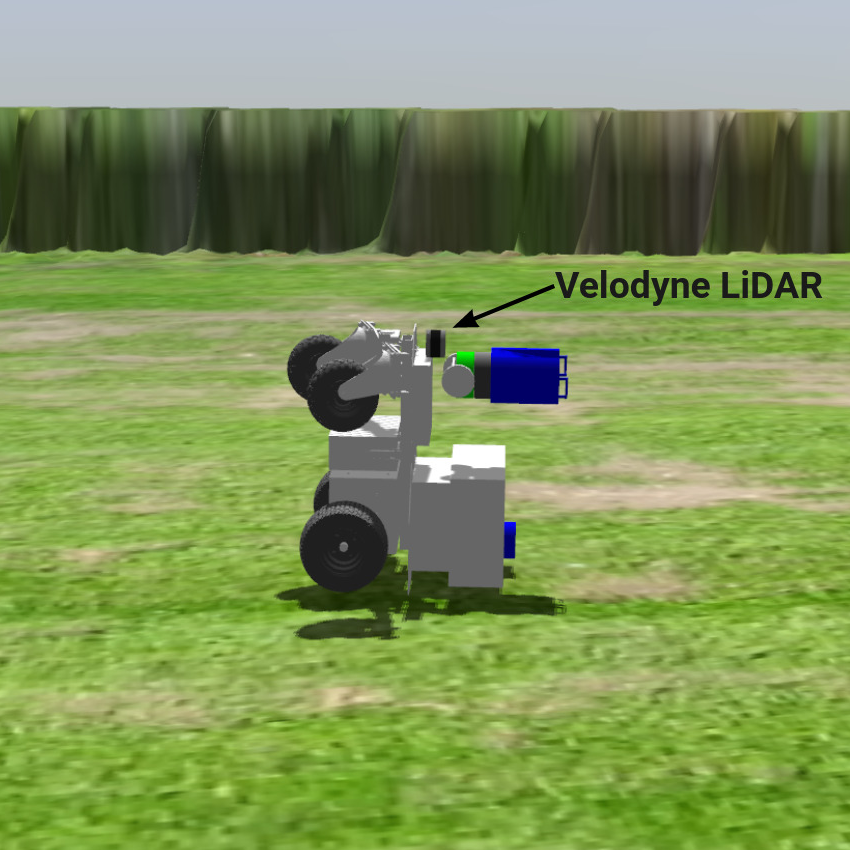
\includegraphics[width=0.8\textwidth]{pics/tilted_AROX.png}
        \caption{\textsc{Tilted AROX in Simulation}}
        \label{fig:tilted_AROX}
    \end{subfigure}
    \hfill
    \begin{subfigure}[b]{0.49\textwidth}
        \centering
        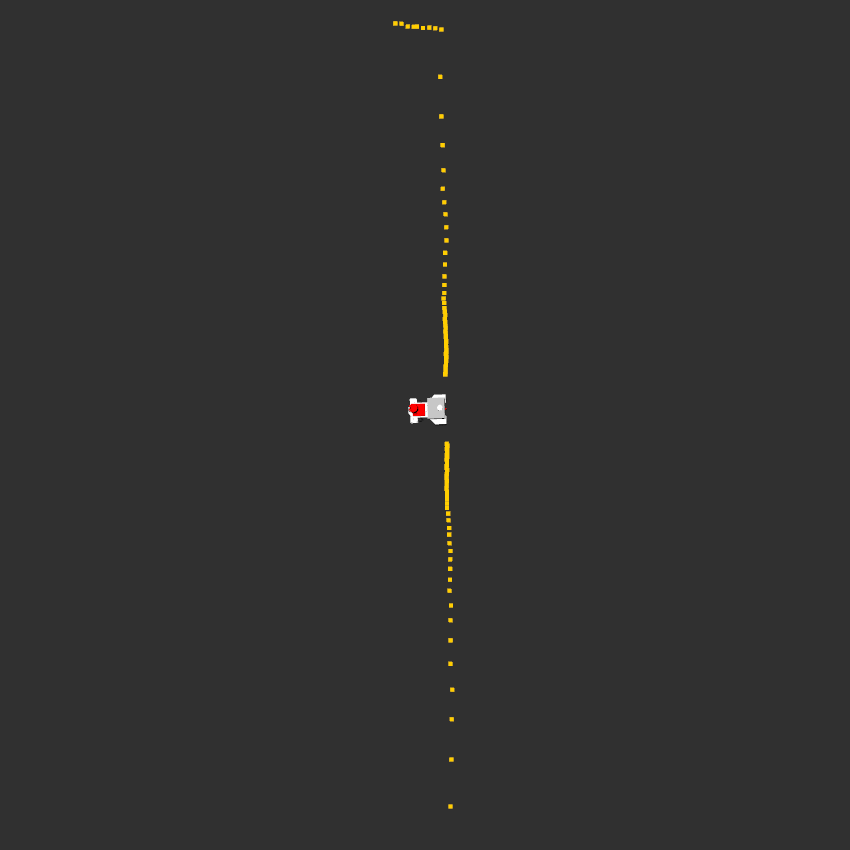
\includegraphics[width=0.8\textwidth]{pics/straight_line.png}
        \caption{\textsc{Feasible Range Values when Facing the Sky}}
        \label{fig:straight_line}
    \end{subfigure}
\caption{\textsc{Experiments with Tilted Sensor}}
\label{fig:prototype_sim}
\end{figure}
\noindent
The monitoring solution implements this approach by calculating the ratio between feasible and infeasible values and comparing it to the lower bound.
If the percentage of feasible range values does not exceed the lower bound, it is considered a sensor failure.
Moreover, it should be detected when no new scans arrive, i.e. the received scan is repeatedly the same.
To be able to compare the newly arrived scan with the previous one, the monitoring node always saves the last scan.
For the actual comparison, a unique hash value is calculated for both scans based on their range values as well as various metadata such as timestamp,
frame identifier, minimum and maximum angle, angle increment, time increment, scan time, and minimum and maximum range.
If the newly arrived scan has the same hash value as the previous one, such a sensor error has been detected.
In general, it is crucial to keep the monitoring solutions as general as possible, i.e. abstract from the specific sensors (\textit{RIEGL}, \textit{Velodyne})
in order to make them reusable for others. One hurdle standing in the way of this claim is the fact that many sensor manufacturers use their own proprietary data types.
Nevertheless, the underlying data is likely to be very similar. To provide some generality, the developed monitoring approaches will be able to handle the two data 
types commonly used in the ROS ecosystem, \code{LaserScan} and \code{PointCloud2}. In all cases, the sensor monitoring node publishes on the topic
\code{/contingency_preemption} with a message that specifies the particular kind of sensor failure and causes a transition to the \code{CONTINGENCY} state.
For a system to use the sensor monitoring node, it must indicate a scan action by publishing on the \code{/scan_action} topic. Additionally, the topic under which the
\code{LaserScan} or \code{PointCloud2} is expected must be configured.\newline

\noindent
The evaluation of a total sensor failure is straightforward, as it can be easily simulated by interrupting the publication of laser scans in the dummy scanning node
described in section \ref{sec:dummy_scanning_node}. The second identified type of sensor failure, i.e. an empty list of range values, is again rather trivial to simulate
by clearing the list of range values before republishing a scan in the dummy scanning node. Scans consisting mainly of impermissible range values can be realized by 
simply manipulating the range values of a scan so that they do not satisfy the maximum and minimum range of the sensor before republishing, i.e. \code{inf}.
Finally, to simulate repeated scans, the dummy scanning node always stores the previous scan and can replace the current scan with the previous one on command.
Accordingly, the simulation of each different sensor fault case is implemented as part of the dummy scanning node introduced in section \ref{sec:dummy_scanning_node},
and can be enabled / disabled via the following ROS topics:
\begin{itemize}
    \item \textbf{total sensor failure} \textrightarrow \code{/toggle_simulated_total_sensor_failure}
    \item \textbf{empty list of range values} \textrightarrow \code{/toggle_simulated_empty_ranges}
    \item \textbf{predominantly impermissible values} \textrightarrow \code{/toggle_simulated_impermissible_ranges}
    \item \textbf{repeated scan} \textrightarrow \code{/toggle_simulated_scan_repetition}\newline
\end{itemize}
Sensor failures of this kind can be addressed with the resolution methods described in section \ref{sec:sensor_failure_resolver}.

\subsection{Lost Connection}
\label{sec:sim_and_mon_lost_connections}

Monitoring and simulation of the specific types of considered connection failures, i.e. WiFi (\ref{sec:sim_and_mon_wifi_connection_problems}), internet
(\ref{sec:sim_and_mon_internet_connection_problems}) and GNSS (\ref{sec:sim_and_mon_gnss_connection_problems}) connection problems (cf. \ref{sec:sim_and_mon_wifi_connection_problems}),
are part of the following sections. However, there is also one monitoring aspect that works identically for all three, namely timeout monitoring. There is a continuously running
procedure that checks the time since the last message from either connection. If a user-specified time limit for one of the connections is exceeded, a contingency 
due to a disconnection is initiated. In general, connection problems can be addressed with the resolution methods described in section \ref{sec:connection_resolver}.

\subsubsection{WiFi Connection Failures}
\label{sec:sim_and_mon_wifi_connection_problems}

The most common form of WiFi failure, which is very relevant and realistic in practice, is of course a simple disconnection.
However, there are again more subtle problems than just the complete absence of a connection, so the quality of an established connection should also be monitored.
Generally, network monitoring can be done arbitrarily detailed, for this work it is limited to some attributes that allow a general statement about the quality of
the connection in practice. One realistic problem is an overall poor link quality, which is a measure combining different kinds of metrics, e.g.
\textit{Received Signal Strength Indication} (RSSI), \textit{Signal to Interference plus Noise Ratio} (SINR), \textit{Packet Delivery Ratio} (PDR), and
\textit{Bit Error Rate} (BER). \cite{Vlavianos:2008} Another well-known problem with WiFi systems is a poor signal, i.e. a low RSSI value. The RSSI is already part of
the link quality assessment, but due to its practical importance, it is also worth to be considered in isolation. Furthermore, the bit rate, i.e. the speed at which
information is transmitted, gives a good indication of the overall connection quality, and it should be recognized when it falls below a certain threshold, which is a
lower limit for practical use. In order to ensure communication with the base station at all times (RTK correction signals, scan storage, etc.), such problems should be
detected and reported or corrected immediately. Of course, the WiFi connection is context-dependent and should be very strong in the proximity of the base station, while it can
be arbitrarily weak out in the field. Nevertheless, for the scenario under consideration, it is assumed that it is available at all times in a certain quality. If this is not the
case in other scenarios, the thresholds can be reconfigured and, if WiFi is not expected to be available at all, the monitoring node can be disabled.\newline
Monitoring for WiFi connectivity problems takes place at two levels of abstraction. From the perspective of the high-level execution monitoring framework developed in this work,
the monitoring is completely independent of hardware and operating system details. However, monitoring the WiFi connection of a particular system depends heavily on such details,
so it is also necessary to provide low-level monitoring for network interfaces. The idea is that the high-level monitoring node expects the information that are evaluated as part 
of the monitoring in a very specific format on the ROS topic \code{/wifi_connectivity_info}. For this purpose, a custom ROS message \code{WiFi.msg} was defined consisting of the
three fields \code{float32 link_quality}, \code{float32 signal_level} and \code{float32 bit_rate}. Therefore, it is irrelevant where this information comes from, it is simply
assumed to be provided. In order to demonstrate the WiFi monitoring in this work, the low-level operating-system-specific monitoring node that transfers this
information to the ROS system is implemented exemplarily for an Ubuntu system. It starts the Unix tool \code{iwconfig}
\footnote{https://manpages.debian.org/bullseye/wireless-tools/iwconfig.8.en.html} as a subprocess for a WiFi interface identifier that can be configured by the user. Subsequently,
the relevant information, i.e. link quality, signal level and bit rate, is parsed from the \code{iwconfig} output for the respective interface and a \code{WiFi.msg} is created
based on this. This message is then published under the \code{/wifi_connectivity_info} topic, which is subscribed by the high-level monitoring node. This process is repeated
continuously every $10$s.\newline
Now that it is clear how the low-level node works, the actual monitoring follows. As mentioned, the high-level monitoring node receives the WiFi information via the ROS topic
\code{/wifi_connectivity_info}. Based on this, the numerical information about the connection is evaluated. If all three provided values are $0$, it is considered
a disconnect and the monitoring solution induces a transition to the \code{CONTINGENCY} state. The link quality is evaluated based on three thresholds: If it is below $5\%$,
it is considered critically poor quality and a transition to \code{CONTINGENCY} follows. For the remaining two thresholds, the quality is not as bad as requiring a contingency
case, but it is still worth notifying the operator. For a link quality of $< 25\%$ a poor quality is reported, and for values less than $50\%$ a below average quality.
The signal level is also monitored based on three thresholds. As introduced in section \ref{sec:sim_and_mon_of_lta_challenges} it gets practically unusable for values below
$-90$ dBm. Thus, $\leq -90$ dBm acts as the trigger for a contingency case. Signal levels of $\leq -80$ dBm and $< -75$ dBm cause notifications of very weak and weak WiFi signals,
respectively. Finally, the bit rate is monitored based on two cases: if it is below $1$ Mb/s, a contingency is triggered, and if it is below $20$ Mb/s, a notification of a
rather low bit rate is transmitted. As soon as a malfunction is detected, monitoring is deactivated and resumed only when the problem has been solved. In all contingency
cases, the high-level WiFi monitoring node publishes on the topic \code{/contingency_preemption} with a message that specifies the particular kind of connection problem.\newline
In summary, the problem of actually detecting the WiFi connectivity on the system in question is completely external to the execution monitoring framework,
which has no operating system coupling at all. There is a layer of abstraction that separates the two views. The assumption of the high-level monitoring framework is the
following: There is a node that publishes the WiFi connectivity for the system every $10$s int the \code{WiFi.msg} format on \code{/wifi_connectivity_info}. If someone wants to use
the execution monitoring framework on Windows, for example, there is no need to modify the framework's code, there just has to be an equivalent WiFi monitoring node for a Windows
system that replaces the Ubuntu-specific one.\newline

\noindent
The simulation of WiFi connection failures is realized by the operating-system-specific implementation of a WiFi monitoring node described in the monitoring section
below. The idea is to simply publish problematic values for each of the considered attributes of the WiFi connection,
i.e. link quality, signal level and bit rate. The simplest case of a complete disconnection is simulated by setting all three values to $0$.
Since the question of which values are considered problematic depends heavily on the environment and application scenario, these values are configurable by the user.
By default, a poor link is simulated by publishing a corresponding value of $2\%$, meaning that the measure of how good the link is described in section
\ref{sec:challenges_for_lta} estimates the quality with only two percent of the optimum. The second attribute, the received signal strength indication (RSSI),
ranges from $-30$ dBm to $-100$ dBm, depending on various aspects, such as distance. \cite{Heurtefeux:2012} The upper bound of $-30$ dBm is the optimal value, which
is almost impossible to achieve in practice, and $-100$ dBm basically means no signal at all. One could roughly classify it as follows: Anything between the optimal
$-30$ dBm and $-67$ dBm can be considered very good in practice, below an RSSI of $-80$ dBm it starts to become critical, and around $-90$ dBm it becomes practically 
unusable. \cite{metageek} Thus, a signal level failure is simulated by publishing an RSSI value of $-90$ dBm. Finally, the default value for a simulated bit rate failure 
is $0.1$ Mb/s. The simulation of each different WiFi fault case can be enabled / disabled via the following ROS topics:
\begin{itemize}
    \item \textbf{poor link quality} \textrightarrow \code{/toggle_simulated_bad_wifi_link}
    \item \textbf{poor signal level} \textrightarrow \code{/toggle_simulated_bad_wifi_signal}
    \item \textbf{poor bit rate} \textrightarrow \code{/toggle_simulated_bad_wifi_bit_rate}
    \item \textbf{disconnection} \textrightarrow \code{/toggle_simulated_wifi_disconnect}
\end{itemize}

\subsubsection{Internet Connection Failures}
\label{sec:sim_and_mon_internet_connection_problems}

Unlike monitoring WiFi connectivity, internet connectivity monitoring does not require an operating system-specific low-level node. The internet bandwidth is tested using the
cross-platform Python tool \code{speedtest-cli}\footnote{https://pypi.org/project/speedtest-cli/}. Nevertheless, for modularization reasons, there is a separate internet
connectivity monitoring node that communicates the internet connectivity properties to the general connectivity monitoring node via the ROS topic \code{/internet_connectivity_info}.
For this purpose, a custom ROS message \code{Internet.msg} was defined consisting of the two fields \code{float32 download_speed} and \code{float32 upload_speed}. Initially,
the connection to the \code{speedtest-cli} API is established. If this fails, an exception is caught and the first type of internet connection problem is detected, namely a
complete disconnect. In such a case, the internet monitoring node creates and publishes an \code{Internet.msg} consisting of an upload and download speed of $0$ Mb/s
reflecting cases of actual disconnects after a successful connection to the API. On the other hand, if the connection to the API was successful, the actual monitoring begins, which
repeatedly performs speed tests every $n$ seconds, where $n$ can be configured by the user. For each result, the download and upload speed is parsed and an \code{Internet.msg} is
generated and published. The high-level connectivity monitor receiving the message performs several checks based on the data. In addition to a check for complete disconnects,
i.e. upload and download of $0$ Mb/s, which causes a contingency, other specific checks are performed. When the download speed $d < 1$ Mb/s, a critically low download speed is 
detected and a contingency is initiated. If $d < 40$ Mb/s, an information is sent to the operator that a rather low download speed was detected. Analogously, the upload speed $u$ is
checked. An upload speed of $u < 1$ Mb/s causes a contingency, and $u < 10$ Mb/s initiates an information of a rather poor upload speed in the communication channel with the human
operator. As always, in all contingency cases, the monitoring node publishes a message on \code{/contingency_preemption} that specifies the particular nature of the connection
problem. In cases of a failed connection to the \code{speedtest-cli} API, the monitoring itself does not work properly, so the connection is reinitialized after the problem is fixed.\newline

\noindent
Simulating internet connectivity problems has three components. First, a total disconnect, which can be simulated by simply cutting the connection or publishing on a prepared topic.
The other two options are again simulated by publishing user-configurable problematic values for the respective download and upload speed components.
By default, a poor download as well as upload speed is simulated by publishing corresponding values of $0.5$ Mb/s.
The simulation of poor download and upload speed cases as well as a total failure can be enabled / disabled via the following ROS topics:
\begin{itemize}
    \item \textbf{disconnect} \textrightarrow \code{/sim_internet_connection_failure}
    \item \textbf{poor download speed} \textrightarrow \code{/toggle_simulated_bad_download}
    \item \textbf{poor upload speed} \textrightarrow \code{/toggle_simulated_bad_upload}
\end{itemize}

\subsubsection{GNSS Connection Failures}
\label{sec:sim_and_mon_gnss_connection_problems}

Unlike the connections considered in the previous two sections, i.e. WiFi and internet (cf. sections \ref{sec:sim_and_mon_wifi_connection_problems} and
\ref{sec:sim_and_mon_internet_connection_problems}), GNSS signals are already part of the ROS world both in the prototype simulation and in practice. The transmission of GNSS data
for both scenarios is shown in fig. \ref{fig:gnss_communication}, where the blue arrows represent the procedure in practice and the red arrows illustrate the case of simulated GNSS
data. In practice, the AROX system as well as the base station (mobile container) use a \textit{u-blox C099-F9P}
\footnote{https://www.u-blox.com/en/product/c099-f9p-application-board?lang=de} application board as GNSS receiver. The board can be configured to transmit or receive RTK correction
signals. Accordingly, the one on board the AROX is configured as RTK-rover and the one mounted inside the base station is configured as RTK-base. The board attached to the AROX is
connected to the on-board computer via USB. Since the on-board computer is an Ubuntu system, the Unix tool
\code{gpsd}\footnote{https://manpages.ubuntu.com/manpages/trusty/man8/gpsd.8.html} can be used, a daemon that can be configured to read the GNSS data from the connected
\textit{u-blox} board. Afterwards, the ROS community package \code{gpsd-client}\footnote{https://wiki.ros.org/gpsd\_client} serves as a bridge between the operating system and the
ROS world. It reads the GNSS data from \code{gpsd} and generates a \code{NavSatFix}\footnote{https://docs.ros.org/en/api/sensor\_msgs/html/msg/NavSatFix.html} message from it, the typical data type for GNSS data in ROS. This message is then published under
the \code{/fix} topic and used for localization, etc. In the simulation scenario (cf. red arrows), \code{GazeboRosGps}, a module from the ROS community package
\code{hector_gazebo_plugins} \footnote{https://wiki.ros.org/hector\_gazebo\_plugins}, is used to simulate GNSS data. It already generates a \code{NavSatFix} message with the
simulated data. However, it does not simulate every single relevant aspect of the GNSS data. It simulates the position and altitude of the robot in \textit{WGS84} coordinates and
also a GNSS velocity vector, but the status, service and covariance information are not generated. This is where the \code{GNSS Simulator} developed as part of this work comes
into play, acting as a \textquote{man-in-the-middle} to enrich the data coming from \code{GazeboRosGps}. For this purpose, it receives the \code{NavSatFix} message from the
\code{/fix_plugin} topic and enriches it with user-configurable service, status and covariance information. Finally, as in the real scenario in practice, a \code{NavSatFix} message
appears on the \code{/fix} topic. Thus, from the perspective of any component that uses the GNSS information, such as localization, it is not clear and also irrelevant whether the
data is real or simulated, the result is the same.
\begin{figure}[H]
    \centering
    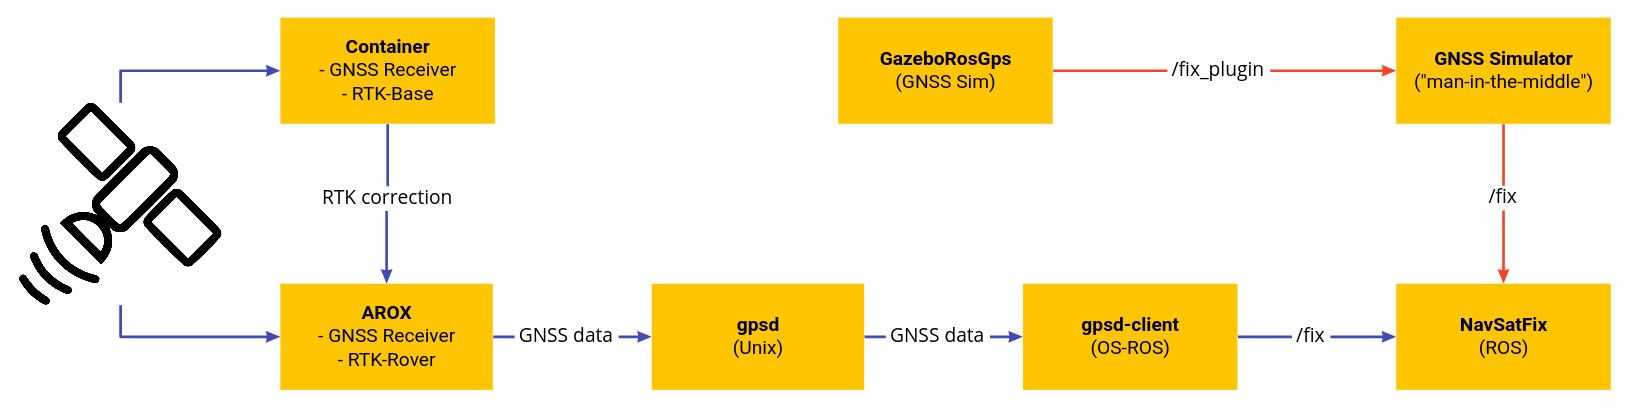
\includegraphics[width=\textwidth]{pics/GNSS_comm.png}
    \caption{\textsc{Processing of GNSS Data (\textbf{\textcolor{myblue}{Practice}} / \textbf{\textcolor{myred}{Simulation}})}}
    \label{fig:gnss_communication}
\end{figure}
\noindent
As can be observed in the processing scheme in fig. \ref{fig:gnss_communication}, the GNSS data arriving at the system,
i.e. received from \code{gpsd}, is already the data potentially corrected by RTK. What is received is the best result there is at the moment; if RTK is available, it will be used.
What is part of the \code{NavSatFix} definition and is also available in \code{gpsd}, i.e. in practice, is the GNSS status with the four possible options \code{STATUS_NO_FIX},
\code{STATUS_FIX}, \code{STATUS_SBAS_FIX}, and \code{STATUS_GBAS_FIX}. The first two options indicate whether or not it was possible to find a position using pure GNSS, e.g.
\textit{GPS}, \textit{GLONASS} or \textit{Galileo}. An SBAS (\textit{Satellite Based Augmentation System}) is a satellite-based system that provides additional real-time data from geostationary
satellites to refine the observations and increase the accuracy, e.g. \textit{StarFire\textsuperscript{TM}}. \cite{Dixon:2006} Hence, the third option indicates whether such
an SBAS was involved in positioning. Analogously, a GBAS (\textit{Ground Based Augmentation System}) aims to ensure integrity and increase accuracy
by using a ground infrastructure consisting of at least two GNSS receivers. \cite{GNSS_aug} Based on this, differential corrections are computed. The fourth option therefore
tells whether a GBAS was utilized during positioning. Essentially, RTK is a specific GBAS system used in practice with the AROX system and the base station. These four GNSS status
options are user-configurable in the \code{GNSS Simulator}. Regardless of whether in simulation or in the case of the real AROX in practice, with the setup described it is always
known if RTK data is currently being received.
Additionally configurable, part of the \code{NavSatFix} message, and given in practice are the service options, i.e. the actual GNSS services used to
retrieve the data, \textit{GPS}, \textit{GLONASS}, \textit{Compass} and \textit{Galileo}. Eventually, the GNSS covariance type as well as the covariances themselves are part of a
\code{NavSatFix} message and thus configurable in the \code{GNSS Simulator}. Covariances are commonly represented as a square matrix $C$ containing the covariance $c_{ij}$ for each pair
of variables $i, j$ in the considered domain $D$. These matrices have the property of being symmetric, that is, the covariance $c_{ij} \in C$ is the same as the covariance 
$c_{ji} \in C$, and provide the variances of the variables on their diagonal, since the covariance $c_{ii}$ of each variable $i \in D$ with itself is equal to the variance of
that variable. The \code{NavSatFix} specification distinguishes different types of position covariances, essentially indicating their reliability.
First, \code{COVARIANCE_TYPE_UNKNOWN} if the GNSS receiver does not yield a quality estimate and the GNSS data should be treated with caution.
\code{COVARIANCE_TYPE_APPROXIMATED} means that the GNSS receiver does not provide covariance values, but instead supplies another quality estimate, such as dilution of precision
(DOP). The covariance values are then approximated based on this estimate. If the GNSS receiver gives at least the variances or standard deviations of the individual measurements,
the type is \code{COVARIANCE_TYPE_DIAGONAL_KNOWN}, since the diagonal contains the variances. For example, assuming the GNSS receiver provides the variances, it is only necessary
to take the square root of the diagonal values to obtain the more meaningful standard deviations. Eventually, \code{COVARIANCE_TYPE_KNOWN} means that the GNSS receiver provides
a rather sophisticated error estimation with a complete covariance matrix of $3 \times 3$ values. The covariances are not directly based on the
current latitude, longitude and altitude belief state, but based on a $2D$ approximation of a small region of the Earth's surface, a tangential plane through the currently believed
position. There are several local tangent plane systems, the specific one assumed in \code{NavSatFix} is the \textquote{East-North-Up} (ENU) coordinate system. Using such a coordinate
system relative to a local origin has the advantage that it allows one to work with intuitive Cartesian coordinates. To give an example, let the locations considered be the 
\textit{Innovation Center Osnabrueck (ICO)} and the \textit{DFKI-Labor Niedersachsen}, shown in fig. \ref{fig:ICO_DFKI_map}. A typical GNSS receiver estimates positions in
geodetic coordinates - latitude (degrees), longitude (degrees), and altitude (meters), e.g. \textit{ICO} $(52.287690, 8.018690, 63.0)$ and \textit{DFKI} $(52.287863, 8.027347, 63.0)$.
Let the ENU representation be constructed with respect to the \textit{ICO} location. This location is the origin of the local coordinate system, i.e. the location where the tangent
plane meets the Earth's surface. The two-dimensional \textquote{east-north-plane}, together with the \textquote{up-axis} perpendicular to the Earth at the reference point, form
the local Cartesian coordinate system. This is, of course, only an approximation that is feasible for relatively small areas, since the Earth's curvature would have to be taken
into consideration for larger areas. Now another location, for instance that of the \textit{DFKI}, is considered. The ENU representation provides the information where this point
of interest is located in the local coordinate system in meters. The result of converting the geodetic coordinates of the DFKI to the ENU system ($590.7, 19.3, 0.0$), is displayed
in fig. \ref{fig:ICO_DFKI_ENU}, i.e. the DFKI is located $590.7 m$ east and $19.3 m$ north of the ICO site. In this case, both locations have the same height.
\begin{figure}[H]
    \centering
    \begin{subfigure}[b]{0.49\textwidth}
        \centering
        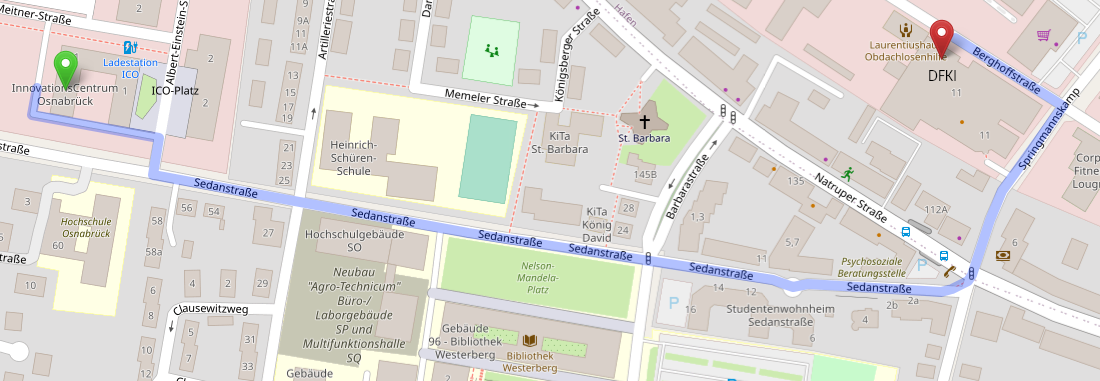
\includegraphics[width=0.8\textwidth]{pics/ICO_DFKI_map.png}
        \caption{\textsc{\textit{OpenStreetMap} Section}}
        \label{fig:ICO_DFKI_map}
    \end{subfigure}
    \hfill
    \begin{subfigure}[b]{0.49\textwidth}
        \centering
        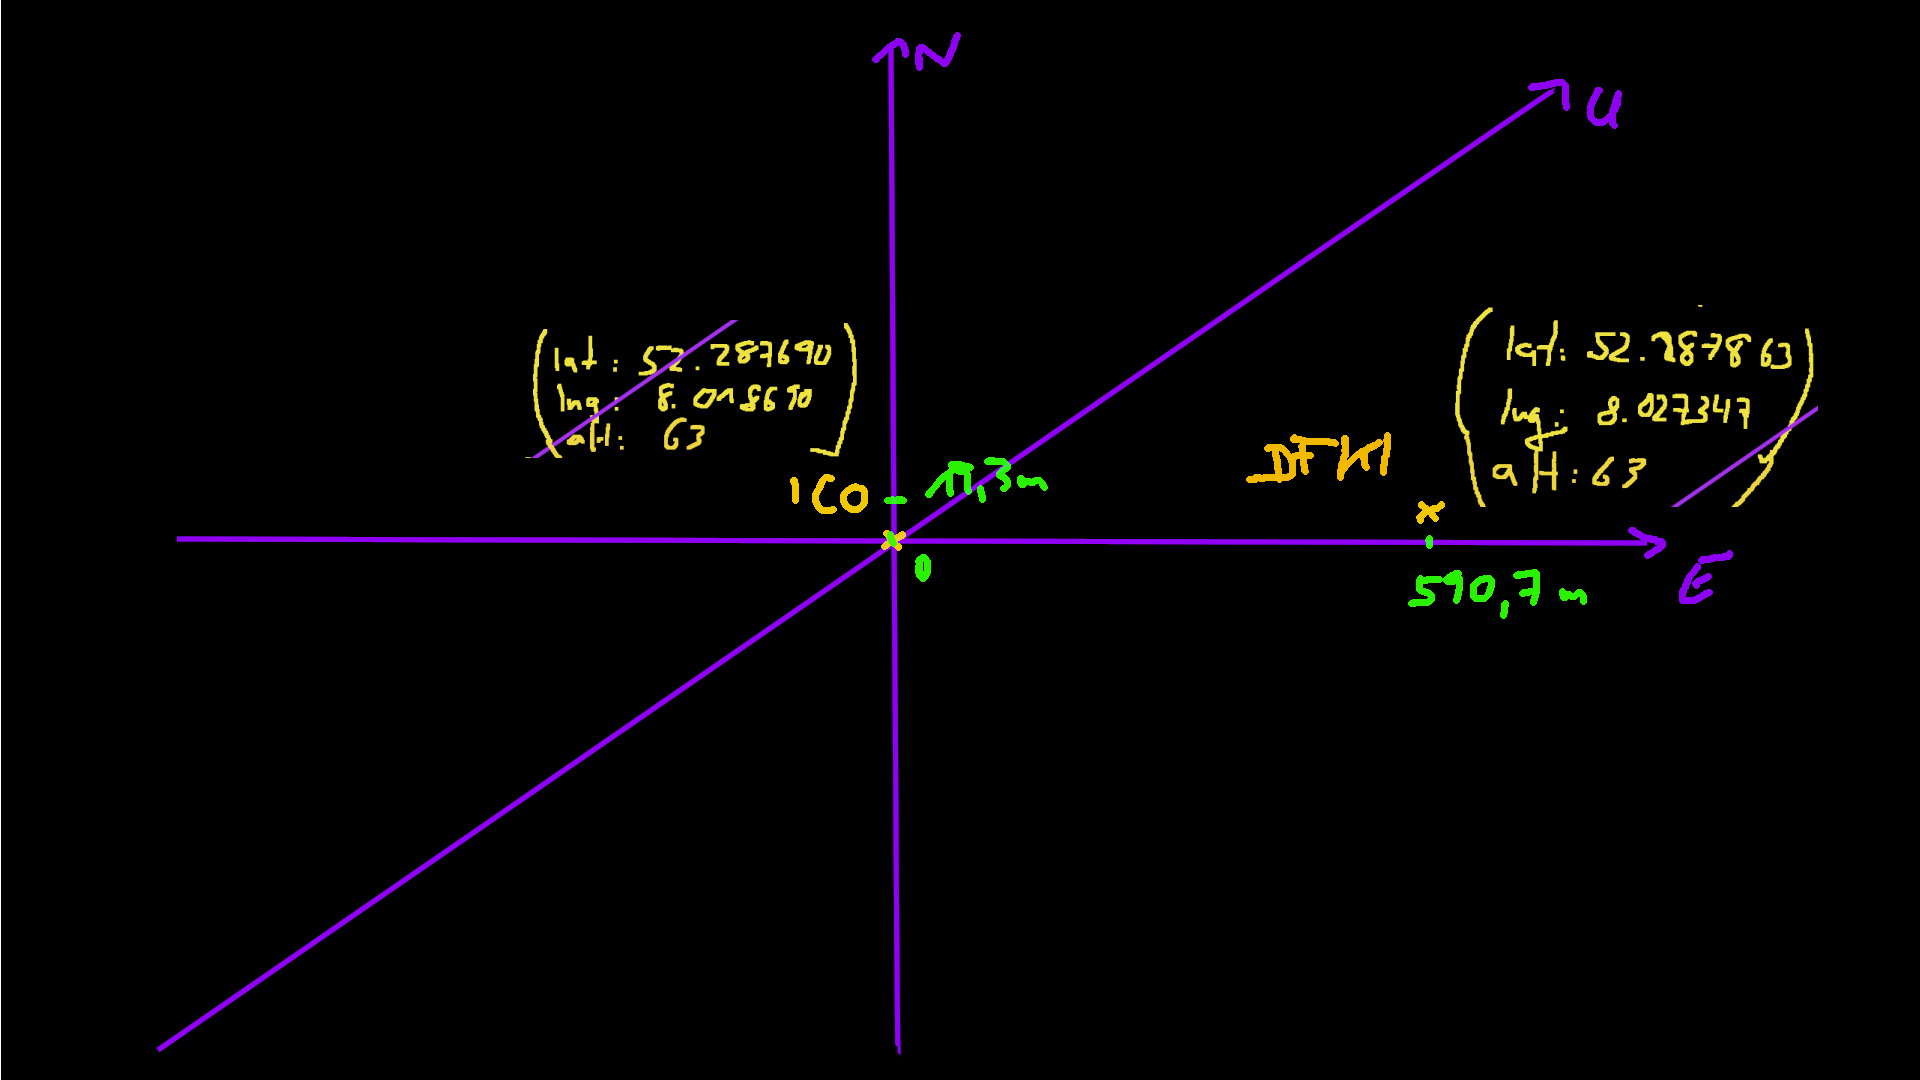
\includegraphics[width=0.8\textwidth]{pics/ICO_DFKI_ENU.png}
        \caption{\textsc{East-North-Up (ENU) Representation}}
        \label{fig:ICO_DFKI_ENU}
    \end{subfigure}
\caption{\textsc{ENU Example} TODO}
\label{fig:ENU_example}
\end{figure}
\noindent
The position covariances $c_{ij}$ in a \code{NavSatFix} message are defined in square meters relative to the tangential plane.
The ENU system is composed of the three variables east ($E$), north ($N$), and up ($U$), i.e. $c_{ij} \in C_{3 \times 3}$ with $i, j \in \{E, N, U\}$.
Thus, one has to consider $\sqrt{c_{ii}} \thinspace \forall \thinspace i \in \{E, N, U\}$ to end up with the standard deviation in meters, i.e. how widely the GNSS approximations are
currently spread in meters. In general, a minor standard deviation implies that the uncertainty about the current estimated position is very low, making the estimate very accurate.
Figure \ref{fig:low_uncertainty}, for instance, shows relatively low positional uncertainty based on standard deviations of $\sqrt{6}m$ in either direction. The violet shape
surrounding the AROX model indicates this uncertainty. In principle, the robot could be anywhere in this shape based on current GNSS data, but the center is currently the most likely
estimated position (the average). Figure \ref{fig:high_uncertainty} shares the same standard deviations for the north and up directions, but has a significantly higher deviation of
$\sqrt{101}m$ in the east direction, resulting in a fairly high uncertainty with respect to this direction.
\begin{figure}[H]
    \centering
    \begin{subfigure}[b]{0.49\textwidth}
        \centering
        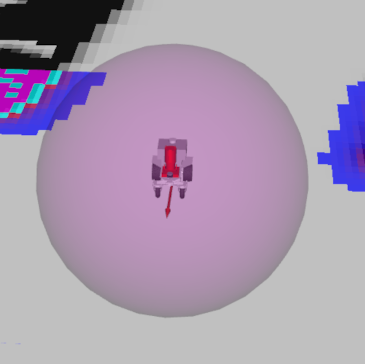
\includegraphics[width=0.5\textwidth]{pics/GNSS_cov_low.png}
        \caption{\textsc{Relatively Low Uncertainty}}
        \label{fig:low_uncertainty}
    \end{subfigure}
    \hfill
    \begin{subfigure}[b]{0.49\textwidth}
        \centering
        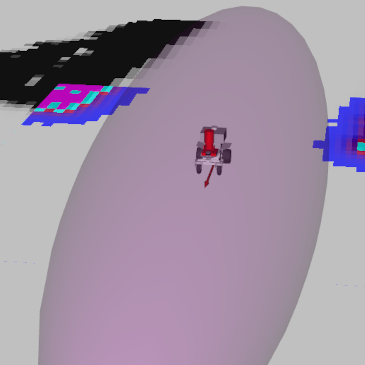
\includegraphics[width=0.5\textwidth]{pics/GNSS_cov_high.png}
        \caption{\textsc{High Uncertainty in One Direction}}
        \label{fig:high_uncertainty}
    \end{subfigure}
\caption{\textsc{Standard Deviations and Uncertainty}}
\label{fig:uncertainty_shape}
\end{figure}
\noindent
Nevertheless, in both cases shown in fig. \ref{fig:uncertainty_shape}, the standard deviations are in the meter range, which is not optimal. With RTK available, the deviations,
i.e. the violet shape, should be much smaller in the centimeter or even millimeter range. It is of some importance to detect and report such changes in position accuracy.
The monitoring for GNSS failures works as follows. First, there is a qualitative assessment of GNSS links that work in principle based on the information in the \code{NavSatFix}
message. If the connection is not perfect, the mission is not immediately interrupted, but it is at least documented.
The quality is rated as high, if the status is \code{STATUS_GBAS_FIX}, i.e. with ground-based augmentation such as RTK, the covariance type is $\geq$ 
\code{COVARIANCE_TYPE_DIAGONAL_KNOWN} (diagonal known or entirely known), and each standard deviation satisfies a user-defined upper bound $d_{max} \in \mathbb{R}_{0}^{+}$,
i.e. $\sqrt{c_{ii}} \leq d_{max} \thinspace \forall \thinspace i \in \{E, N, U\}$. The last entry of the matrix, i.e. $c_{UU} \in C$ , may not always be present, so
$c_{UU} \in \mathbb{R}_{0}^{+} \cup \emptyset$. It is classified as tolerable if the status is $\geq$ \code{STATUS_FIX}, the covariance type is $\geq$
\code{COVARIANCE_TYPE_APPROXIMATED}, and the standard deviations in turn satisfy $d_{max}$. 
Finally, it is classified as low if it provides a position belief state ($\geq$ \code{STATUS_FIX}), but the covariance
type is unknown. So much for the qualitative assessment of a GNSS link that works in principle.\newline
The first type of monitoring for real failures that interrupt \code{NORMAL_OPERATION} is the status monitoring.
If the status is not set to one of the available options (\code{STATUS_NO_FIX}, \code{STATUS_FIX},
\code{STATUS_SBAS_FIX}, \code{STATUS_GBAS_FIX}), a contingency is initiated, i.e. a message on \code{/contingency_preemption} interrupts the normal operation.
Furthermore, if the status is \code{STATUS_NO_FIX}, the GNSS system was unable to find the position, which is certainly a problem for localization that causes a contingency
case. Status monitoring also checks for cases of \code{STATUS_FIX}, which means that pure GNSS was used for positioning and no RTK is available. However, this is not a reason for
contingency, just information worth publishing on \code{/robot_info}. What is also worth reporting, but does not trigger a contingency, is an unknown service, i.e. when the
\code{NavSatFix} message does not contain any of the available GNSS services \textit{GPS}, \textit{GLONASS}, \textit{Compass} or \textit{Galileo}. Again more critical is the latitude ($lat$) / longitude ($lng$) belief state
monitoring. It is ensured that both values are present and satisfy their respective domains, i.e. $lat \in [-90\degree, 90\degree]$ and $lng \in [-180\degree, 180\degree]$. Altitude is not taken into account
because many GNSS receivers do not provide this information. Eventually, there is uncertainty assessment, i.e. covariance monitoring. 
First, it is checked whether the covariance type corresponds to one of the
available options (\code{COVARIANCE_TYPE_UNKNOWN}, \code{COVARIANCE_TYPE_APPROXIMATED}, \code{COVARIANCE_TYPE_DIAGONAL_KNOWN}, \code{COVARIANCE_TYPE_KNOWN}). Otherwise,
a notification is sent to the operator, but of course not a contingency, as this is not critical. The most meaningful components of the covariance matrix are the variances or, more
precisely, the standard deviations, i.e. the square root of the diagonal values, because they actually provide information about the accuracy of the estimated position.
As for the actual standard deviation values, two things can be observed: The absolute values (appropriate / too high) and their progression over time.
The latter is implemented as a variance history in the form of a fixed-length list that always stores the diagonals of the last $n \in \mathbb{N}$
covariance matrices and performs a list shift in which the oldest one is removed when a new one arrives. The length $n$ is again configurable by the user. In the analysis of the variance
history, the square roots, i.e. the standard deviations, are considered, since, as mentioned, these are the crucial values provided by many GNSS receivers.
Whenever the covariance type of an incoming \code{NavSatFix} message is $\geq$ \code{COVARIANCE_TYPE_DIAGONAL_KNOWN}, the history is updated. On the arrival of new feasible 
messages, the deviation progression is analyzed. Such an analysis primarily examines the standard deviations of the east and north components, but also those of the upward component,
if present. First, it is checked whether the history contains only increasing values for the respective component. If this is the case and, in addition, the difference between the
oldest and the newest deviation is greater than a user-defined significant deviation increase $d_{inc} \in \mathbb{R}_{0}^{+}$, a contingency is initiated. Thus, the definition of a
bad deviation progression is exclusively increasing values together with an overall absolute increase between the oldest and latest value that exceeds a certain threshold.
Finally, there is one last check, which relates to the absolute values. If the type is $\geq$ \code{COVARIANCE_TYPE_DIAGONAL_KNOWN}, the present variances 
$c_{ii} \in \mathbb{R}_{0}^{+} \thinspace \forall \thinspace i \in \{E, N, U\}$ can with a clear conscience be used for quality assessment. If any of the standard deviations exceeds the user-specified maximum deviation threshold $d_{max}$,
i.e. $\exists \thinspace c_{ii}, i \in \{E, N, U\} : \sqrt{c_{ii}} > d_{max}$, normal operation is interrupted by publishing to \code{/contingency_preemption}. 
If the type is \code{COVARIANCE_TYPE_APPROXIMATED}, the variances can be considered, but with caution, without giving it too much weight.
The standard deviations $\sqrt{c_{ii}} \in C \thinspace \forall \thinspace i \in \{E, N, U\}$ are checked, but high values exceeding the threshold do not cause a contingency, only a message on \code{/robot_info}.
In principle, it would also be useful to monitor the off-diagonal elements of the covariance matrix, i.e. the actual covariances, since these elements provide information about the
reciprocal relationship of the directions under consideration. For instance, if $c_{NE} < 0$, a negative deviation in the north direction is likely to be matched by a positive deviation in
the east direction, and vice versa. However, in the scope of this work, the monitoring of the covariance matrix will be limited to the above cases. It is crucial that the approaches
are essentially compatible with all systems using \code{NavSatFix} and are not limited to the AROX system or the present scenario. Hence, for a system to use GNSS monitoring, it simply needs
to publish \code{NavSatFix} messages on \code{/fix}.\newline

\noindent
As before, evaluation of potential problem cases as well as monitoring procedures requires simulation of such cases, which is performed in the \code{GNSS Simulator} described above.
The timeout failure can be easily simulated by unsubscribing the \code{/fix_plugin} topic for a period of time that exceeds the time limit. Quality estimation can be evaluated by
simply configuring the status, covariance information, and service according to the above definition. Monitoring of status, service and position belief state can be simulated by
setting inappropriate values for each. Likewise, absolute deviation monitoring as well as variance history analysis can be tested by simulating the respective problems.
Let the type be \code{COVARIANCE_TYPE_DIAGONAL_KNOWN}, the user-specified history length $n = 4$, and the deviation increase threshold $d_{inc} = 5 m$. Deviation monitoring
can then be tested by publishing the following (co)variance progression ($n = 4$ messages in sequence):
\begin{figure}[H]
    \begin{subfigure}[b]{0.24\textwidth}
    \centering
        $\left(
        \begin{array}{rrr}
        \boldsymbol{16.2} & 0.0 & 0.0 \\
        0.0 & \boldsymbol{4.4} & 0.0 \\
        0.0 & 0.0 & \boldsymbol{16.5} \\
        \end{array} \right) $
        \caption{\textsc{}}
        \label{fig:oldest}
    \end{subfigure}
    \hfill
    \begin{subfigure}[b]{0.24\textwidth}
    \centering
        $\left(
        \begin{array}{rrr}
        \boldsymbol{25.1} & 0.0 & 0.0 \\
        0.0 & \boldsymbol{9.8} & 0.0 \\
        0.0 & 0.0 & \boldsymbol{16.8} \\
        \end{array} \right) $
        \caption{\textsc{}}
        \label{fig:}
    \end{subfigure}
    \hfill
    \begin{subfigure}[b]{0.24\textwidth}
    \centering
        $\left(
        \begin{array}{rrr}
        \boldsymbol{89.0} & 0.0 & 0.0 \\
        0.0 & \boldsymbol{64.2} & 0.0 \\
        0.0 & 0.0 & \boldsymbol{81.3} \\
        \end{array} \right) $
        \caption{\textsc{}}
        \label{fig:}
    \end{subfigure}
    \hfill
    \begin{subfigure}[b]{0.24\textwidth}
    \centering
        $\left(
        \begin{array}{rrr}
        \boldsymbol{99.4} & 0.0 & 0.0 \\
        0.0 & \boldsymbol{77.7} & 0.0 \\
        0.0 & 0.0 & \boldsymbol{98.3} \\
        \end{array} \right) $
        \caption{\textsc{}}
        \label{fig:latest}
    \end{subfigure}
\caption{\textsc{(Co)variance History (old to new)}}
\label{fig:cov_history}
\end{figure}
\noindent
The (co)variance progression depicted in fig. \ref{fig:cov_history} is expected to cause a contingency for various reasons, e.g. due to the fact that the history only
contains increasing standard deviation values for the east component ($\sqrt{16.2} m \rightarrow \sqrt{25.1} m \rightarrow \sqrt{89.0} m \rightarrow \sqrt{99.4} m$) and the overall
absolute increase between the east deviation of the oldest (cf. fig. \ref{fig:oldest}) and latest (cf. fig. \ref{fig:latest}) covariance matrices exceeds the defined threshold
of $5 m (\approx 5.95 m)$. It is reasonable to interrupt normal operation in such a case, as such a (co)variance progression poses great challenges for localization.
The simulation of the GNSS failure cases can be enabled / disabled via the following ROS topics:
\begin{itemize}
    \item \textbf{disconnect / timeout} \textrightarrow \code{/toggle_simulated_timeout_failure}
    \item \textbf{good quality} \textrightarrow \code{/set_simulated_good_quality}
    \item \textbf{medium quality} \textrightarrow \code{/set_simulated_med_quality}
    \item \textbf{low quality} \textrightarrow \code{/set_simulated_low_quality}
    \item \textbf{unknown status} \textrightarrow \code{/set_simulated_unknown_status}
    \item \textbf{no fix} \textrightarrow \code{/set_simulated_no_fix}
    \item \textbf{no RTK} \textrightarrow \code{/set_simulated_no_rtk}
    \item \textbf{unknown service} \textrightarrow \code{/toggle_simulated_unknown_service}
    \item \textbf{infeasible lat / lng} \textrightarrow \code{/toggle_simulated_infeasible_lat_lng}
    \item \textbf{variance history failure} \textrightarrow \code{/toggle_simulated_variance_history_failure}
    \item \textbf{high deviation} \textrightarrow \code{/toggle_simulated_high_deviation}
\end{itemize}

\subsection{Data Management}
\label{sec:sim_and_mon_data_management}

Similar to sensor (perception) monitoring, executing a \code{scan} action launches the data monitoring procedure, which looks for the potential data management issues presented in
section \ref{sec:challenges_for_lta}. To perform the drive capacity check, i.e. to determine whether the drive on which scan logging or data storage in general takes place has enough
free space, the cross-platform library \code{psutil}\footnote{https://pypi.org/project/psutil/} is used. It provides a function \code{disk_usage()} which returns the load of the
specified disk, e.g. the one configured in \code{MONITOR_DRIVE}. Unlike WiFi connection monitoring, where the actual low-level network connectivity checks are outsourced
from the monitoring framework due to its operating system coupling, disk capacity checks can be part of the framework itself because of the cross-platform nature of \code{psutil}.
If the result of \code{disk_usage(MONITOR_DRIVE)} exceeds $99\%$, the node detects a full memory and causes an interruption of the robot's mission and a transition to the
\code{CONTINGENCY} state. Additionally, notifications are sent to the operator when the disk load exceeds $95\%$ and $90\%$, with an indication that the data should be backed up
externally soon. So much for very general data management monitoring, which in principle can be used for all types of data acquisition tasks, since the type of data is irrelevant
to capacity testing. There is also a more scenario-specific part based on certain assumptions and dependencies that is optional and can be enabled or disabled by the user.
This is the specific scan logging monitoring that assumes that the data acquisition task at hand is a scanning task, such as the one described in section
\ref{sec:lta_plant_observation}, and that the scans are written to a user-configured directory in a file published by the dummy scanning node described in section
\ref{sec:dummy_scanning_node}. Since the data format of the scans written by the dummy scanner is well-known, i.e. \code{LaserScan} or \code{PointCloud2}, the entries logged in
this log file can be easily evaluated. The idea is that there should be an additional scan entry in the log file after a successful scan action. If that is not the case,
a data management error has been detected and a transition to \code{CONTINGENCY} is initiated. It would also be possible to implement some sort of exception escalation system
based on sensor logging errors, but since this would require in-depth knowledge of implementation details of the sensors used, it was renounced.\newline
General capacity monitoring is based on the idea of not having dependencies on specific scenarios or configurations, and instead just monitor the configured path and communicate
when certain thresholds are exceeded, which, as mentioned, basically works for any data acquisition task. However, the goal of ensuring a certain level of generality applies to
both cases. Of course, the second case is only suitable for laser scanning tasks, but it is not limited to one specific sensor. It can deal with all kinds of sensors that provide
results in the form of \code{LaserScan} or \code{PointCloud2}, which covers quite some generality. Therefore, a specific sensor such as the \textit{RIEGL} (cf. fig.
\ref{fig:arox_system}) can be replaced by another model without any problems, and data monitoring should continue to work based on the slight constraint of producing data of the
two mentioned types. General capacity monitoring works either way. Since the logging of the data always follows the scanning and the scanner is the module that writes the scans to
the file system, it would be superfluous to check the data again for plausibility, as this is already part of the sensor monitoring. It suffices to verify whether the storing
operation, i.e. writing the scan to the log file, worked. Moreover, it is worth noting that a total sensor failure always implies a data management failure of the second type,
but this should already be detected by the sensor monitoring procedure. Of course, more checks could be made for scenario-specific logs on the drive, etc., but since this would
require additional knowledge of the specific circumstances, it would violate the goal of being as general as possible. Nevertheless, it is possible to extend data management in
the future to include application-specific monitoring aspects that can be easily disabled to maintain general applicability. For a system to use the data management monitoring node,
it must indicate scan actions via \code{/scan_action} and their completion via \code{/scan_completed}. Furthermore, \code{MONITOR_DRIVE} as well as \code{SCAN_PATH} need to be
configured.\newline

\noindent
It is not a big challenge to simulate the occurrence of the data management problems presented in section \ref{sec:challenges_for_lta}. To simulate a ``full disk''-failure,
i.e. a full memory of the drive on which the scans are to be logged, one could simply prepare a full USB flash drive and configure the path to be monitored accordingly,
e.g. mount flash drive to \code{/mnt/usb} and set \code{MONITOR_DRIVE = /mnt/usb}. It is also implemented in such a way that one can simply prepare the flash drive and later publish
to \code{/sim_full_disk_failure}, which will then set the \code{MONITOR_DRIVE} to \code{/mnt/usb}. The second and more scenario-specific type of error is the scan logging error,
which can be simulated by simply not writing the scan to the file system in the dummy scanning node introduced in section \ref{sec:dummy_scanning_node}. Simulation of this type
of error can be enabled / disabled via the ROS topic \code{/toggle_simulated_scan_logging_failure}. Data management issues can be addressed with the resolution methods described
in section \ref{sec:data_management_resolver}.

\subsection{Plan Deployment Failure}
\label{sec:sim_and_mon_plan_deployment_failures}

There are several potential failures regarding the deployment of generated plans. The first and most apparent is a missing plan, i.e. a situation where the robot is ready in
principle to perform a mission, but no plan arrives and it remains in the \code{IDLE} state. Since this is not an error per se and this case may be perfectly valid, once a certain
threshold is exceeded, it merely triggers a notification via \code{/robot_info} to the human operator and keeps notifying at a specified frequency. The information whether a plan
has been received, i.e. a mission is being executed, is retrieved via a configurable topic, in the scenario described in section \ref{sec:prototype_scenario} via
\code{arox/ongoing_operation}. Additionally, the \code{PlanDeploymentMonitor} subscribes to a topic \code{/plan_retrieval_failure} on which the embedded low-level operation state
machine publishes as its normal error treatment behavior in case of plan retrieval failures, e.g. exceptions. There are defined error codes published on this topic ($0$: plan
retrieval service unavailable, $1$: empty plan, $2$: infeasible plan). Based on this error code, the \code{PlanDeploymentMonitor} initiates a contingency with an appropriate message
explaining the reason, using the \code{/contingency_preemption} topic. Monitoring of plan deployment failures is
therefore a special case, since most of the monitoring is based on error handling reported by the operational state machine. However, this makes sense because these errors are
naturally detected in the operation state machine and only need to be reported or passed on to the higher-level state machine for execution monitoring. Brodskiy et al. refer to these
types of failures recognized and indicated within a component as \textit{signaled failures} and argue that it is desirable to cover as many aspects as possible by such signaled
failures, with each component being more or less self-responsible. \cite{Brodskiy:2011}
The exact error treatment responsible for detecting these errors works as follows. First, the plan generation node described in section \ref{sec:plan_generation} provides plans via the
\code{arox_planner/get_plan} service. If a call to this service triggers a timeout exception, it gets caught, the error is reported (code $0$), and the operation state machine
remains in the \code{IDLE} state. Analogously, a plan with an empty list of actions (code $1$) and a plan containing an action of an unknown type (code $2$) are recognized and
reported. The detection of actions of an unknown type is based on a configurable list of actions that are expected, e.g.. \code{drive_to}, \code{return_to_base}, \code{charge}
and \code{scan} in the considered scenario. In order to allow the monitoring node to initiate the contingency without the operational state machine immediately transitioning back
to \code{IDLE} and repeatedly requesting a plan, a short delay (e.g. $1s$) is introduced for each detected problem to avoid unnecessary timing conflicts during transitions.
Thus, in order for other systems to be able to use the plan deployment monitoring, the mentioned topics and the action list must be configured. Moreover, explicit errors can be
communicated via \code{/plan_retrieval_failure} using the described error codes.\newline

\noindent
For simulation, it is quite obvious that it is reasonable to simulate the failures where they occur, i.e. in the plan generator (cf. section \ref{sec:plan_generation}). The
situation of an extended idle time is simulated by simply blocking the plan fetch for a configurable period of time, which must be greater than or equal to the threshold defined
in \code{PlanDeploymentMonitor}. The simulation of an unavailable plan service is done by temporarily shutting down the service using the \code{shutdown} method provided by ROS services.
Empty and otherwise infeasible plans are trivially simulated by either clearing the list of actions or setting one of the action names to an unspecified string.
The simulation of the plan deployment failure cases can be enabled via the following ROS topics:
\begin{enumerate}
    \item \textbf{extended idle time} \textrightarrow \code{/sim_extended_idle_time}
    \item \textbf{unavailable plan service} \textrightarrow \code{/toggle_unavailable_plan_service}
    \item \textbf{empty plan} \textrightarrow \code{/sim_empty_plan}
    \item \textbf{infeasible plan} \textrightarrow \code{/sim_infeasible_plan}
\end{enumerate}
\noindent
Plan-deployment-related challenges for LTA can be addressed using the resolver described in section \ref{sec:plan_deployment_resolver}.

\subsection{Navigation Failure}
\label{sec:sim_and_mon_navigation_failures}

Since the identified challenges of \textit{Obstacles Blocking the Planned Path} and \textit{Sustained Recovery} are also essentially navigation problems, the three challenges are
considered together under the heading \textit{Navigation Failure}. Although sustained recoveries could in principle refer to all kinds of problems, this thesis is limited to
sustained recoveries in the case of navigation problems, as this is by far the most relevant case from a practical perspective. Thus, it is sustained recoveries initiated by
\code{move_base_flex}.\newline
Recovery behaviors should naturally vary between static and dynamic obstacles. A dynamic obstacle like a person or an animal will in most cases simply walk through the scene and
disappear a moment later, so waiting for a moment can already be a very reasonable and sufficient recovery behavior. Static obstacles, on the other hand, may be present for longer
periods of time, requiring more sophisticated recovery behaviors. \code{move_base_flex} is generally already able to detect obstacles. The task of a monitoring procedure in this
case is to closely observe what \code{move_base_flex} is doing and intervene if necessary. Concerning the obstacles, there are two distinct cases: Either the obstacles only block
the direct path, but there is still one, or the obstacles actually block every single path and the robot cannot reach its destination. In the first case, it would be preferable if
the robot was able to find it, but if it is incapable of doing so, it should be detected and communicated. This is basically the case of navigation failures in the sense that there
is a path to the navigation goal, but \code{move_base_flex} cannot find it (cf. fig. \ref{fig:nav_fail}). Fig. \ref{fig:nav_fail} shows a side by side comparison of what the robot
perceives and the actual section of the simulated world. In fig. \ref{fig:nav_fail_rviz} the route currently considered by \code{move_base_flex} is depicted (green line) as well as the
target pose (cyan arrow). Examining the actual world excerpt in fig. \ref{fig:nav_fail_gazebo}, it is obvious that this route will not lead the robot to its destination. However, as
can be observed from fig. \ref{fig:nav_fail_gazebo}, there is a viable route (red line) that would accomplish this. In some cases, \code{move_base_flex} may find the viable route after a while,
but this is not assured. The problem in such cases is often that the viable routes are somehow counterintuitive, e.g., because they require a detour, at least given the robot's partial
knowledge of the environment. Analogous to leaving local optima in optimization, in some circumstances the robot must first navigate farther away from the target before it can actually
reach it.
\begin{figure}[H]
    \centering
    \begin{subfigure}[b]{0.49\textwidth}
        \centering
        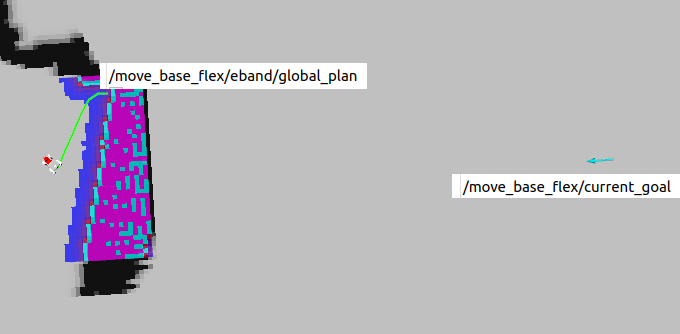
\includegraphics[width=\textwidth]{pics/nav_fail_wrong_route_0.png}
        \caption{\textsc{Considered Route (rviz)}}
        \label{fig:nav_fail_rviz}
    \end{subfigure}
    \hfill
    \begin{subfigure}[b]{0.49\textwidth}
        \centering
        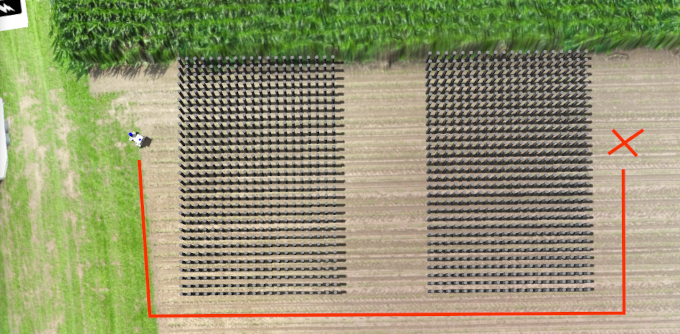
\includegraphics[width=\textwidth]{pics/nav_fail_wrong_route_1.png}
        \caption{\textsc{Feasible Route (Gazebo)}}
        \label{fig:nav_fail_gazebo}
    \end{subfigure}
\caption{\textsc{Navigation Failure - Unable to Find a Path to the Goal}}
\label{fig:nav_fail}
\end{figure}
Such examples are by no means contrived, it is not unrealistic that the robot will regularly face such situations in practice, i.e. it is important to recognize them and enable
the system to cope with them. To give an example from the scenario under consideration: An unexpected obstacle could block the path of the robot, e.g. a large agricultural machine. 
If the local costmap, which is usually between $3 \times 3$ and $5 \times 5$ meters, is smaller than the obstacle, this problem arises. The keyword here is \textit{sensor horizon},
if it is too small it can lead to problems like this. On the other hand, it should be as small as possible to save runtime and increase efficiency. In general, the problem arises
from the fact that \code{move_base} and \code{move_base_flex} work with two layers, i.e. two maps, the global map where everything is static and known, and the local map for dynamic
obstacles, which is initially empty. Now back to the example of the agricultural machine blocking the robot's path. Since this machine is not a static object that is part of the
global map, it can only be recognized as part of the local map. However, the local costmap shows a section of the machine that is at most as large as the local costmap. Moreover,
everything that leaves the local costmap is \textquote{forgotten} by the robot. This leads to absurd situations in which the robot drives along the obstacle and forgets about it when
parts of it leave the sensor horizon, so that the path behind it appears clear again. Thus, the robot oscillates back and forth in an endless loop. A simple workaround, which is not
a panacea but is practically used in the considered scenario, is to simply copy information from the local map to the global map so that the local obstacles can be taken into
account in the global planning (\code{move_base_flex}). This assumes that everything the robot perceives locally is transferred to the static global costmap so that it is henceforth
considered static. This approach misuses the global static map as a knowledge store for local sensor information. However, not persistently, but only as working memory, only during
the runtime of the robot. An obvious problem is that this assumption does not hold, since in this approach dynamic obstacles such as people can be erroneously entered into the global
map and henceforth be considered static obstacles. This happens when a person remains stationary until leaving the sensor horizon of the robot. Nevertheless, since such cases are much
rarer compared to the first issue, this workaround proved to be practically useful in this particular context. In the long term, of course, a more sensible solution must be developed.\newline
So much for situations that can be solved in principle. In the other case (obstacles block every single path), however, it should be detected and communicated in any case, because the robot can not solve it itself. If the robot is unable to successfully generate a
path, there are essentially two different outcomes, regardless of whether this is because there is no path or because it simply cannot find it. First, it results in a sustained
recovery. Second, it simply fails with an error and aborts the navigation target. Both cases should be recognized. During practical experiments in this work, there were many
situations where \code{move_base_flex} was unable to find a correct path and simply ended up in a loop of failed recoveries without ever returning to normal operation. In this
case, the robot should try a few different recovery actions and then abort and report the problem. Monitoring methods must therefore track the results / states of recovery
behaviors and decide whether it is appropriate to try more or stop. To identify sustained recovery situations, it is necessary to count them somehow. \code{move_base_flex}
communicates its status via the ROS topic \code{move_base_flex/exe_path/status}. Consequently, to count the number of failed recoveries, one can simply count the transitions
from \code{GoalStatus.ACTIVE} to \code{GoalStatus.ABORTED}. \code{GoalStatus.SUCCEEDED} should always reset the counter, because then the recovery has actually solved the problem.
Monitoring is performed at a frequency specified by the user and verifies the current recovery count $r \in \mathbb{N}$. Whenever $r = 1$, i.e. when the first recovery occurs after successful
operation, the current position of the robot is stored using the GNSS data obtained from the \code{/fix} topic (cf. section \ref{sec:sim_and_mon_gnss_connection_problems}). If the
recovery count reaches a user-configurable recovery limit $l \in \mathbb{N}$, i.e. $r \geq l$, a contingency is initiated via \code{/contingency_preemption} due to a sustained recovery. This method covers a sustained recovery, as it
arises from a case of obstacles without the possibility of circumvention. Combined with a check for explicit \code{move_base_flex} errors, this covers all expected navigation failures, since
they will all end with a persistent recovery or an explicit termination. The explicit check works as follows. The navigation monitoring node maintains a subscription to
\code{/explicit_nav_failure} through which external procedures, such as the low-level operation state machine, can trigger a contingency due to a navigation problem. For this
purpose, the operation state machine publishes to \code{/explicit_nav_failure} and notifies the monitoring procedure whenever a navigation goal issued to
\code{move_base_flex} explicitly returns \code{GoalStatus.ABORTED}. This is again an example of \textit{signaled failures} proposed by Brodskiy et al. \cite{Brodskiy:2011} and
discussed earlier in section \ref{sec:sim_and_mon_plan_deployment_failures}.
One problem is that repeated recoveries in which some progress is actually achieved should not be mistaken as
sustained recoveries and thus failure. Hence, one should not only count the repetitions and declare that it has failed after a number of unsuccessful attempts, i.e. $r \geq l$, but
also take into account reasonable progress towards the goal. For instance, if the robot approaches the target during the process rather than just rotating on the spot, it should be
viable. For this purpose, each time $r \geq l$, a further check is performed before a contingency is triggered, namely comparing the stored position of the robot at the beginning of
the recovery sequence with the present position. If the distance between the two locations is less than a user-configurable lower bound, the robot has not made sufficient progress
and a contingency is initiated. Otherwise, the robot has performed a number of recoveries, but with some success as it progresses towards the goal, so this is not considered a
failure. In such cases, the operator is informed via \code{/robot_info}, the recovery counter is reset, i.e. $r = 1$, the initial recovery position is set to the present position
and the recovery process can be continued.
It is important to note that monitoring is kept as generic as possible to be compatible with other scenarios and applications involving autonomous mobile robots.
For instance, it is easy to switch to the common navigation framework \code{move_base} by simply changing the topic configuration.
The counting of transitions etc. should still work, because \code{move_base} works with the same \code{GoalStatus} information.
Essentially, any navigation framework that is compatible with the general \code{actionlib_msgs/GoalStatus} is compatible with the introduced monitoring solution.
For a system to use the navigation monitoring node, it simply needs to specify the \code{GOAL_STATUS_TOPIC} under which the \code{GoalStatusArray} messages appear. Additionally,
\code{NavSatFix} messages are again expected to appear on \code{/fix} to track progress in cases of sustained recovery. As described, the topic \code{/explicit_nav_failure} can be
used to report explicit navigation errors. Of course, it would be possible to simply extend the \code{move_base_flex} state machine to perform this type of monitoring, but doing so
would only solve the problem for a specific framework, which would contradict the claim of achieving some generality.\newline

\noindent
Sustained recoveries as well as explicit \code{move_base_flex} failures can be evaluated in simulation by inducing situations where recovery is not possible, e.g., when the
path to the destination is blocked and there is no other way, i.e., by specially constructed examples that are particularly difficult for the navigation algorithms to solve.
The occurrence of static and dynamic obstacles can be implemented in the simulation by spawning mobile and immobile objects at randomized positions that could potentially block
the robot's path. However, as mentioned earlier, dynamic obstacles are generally not a major concern as they will appear as obstacles, initiate a recovery, usually a turn on the
spot, and after that, in most cases, the obstacle has already disappeared and the robot can continue its mission. If this is not the case, it could be treated as static anyway.
Therefore, only the harder case of unexpected static obstacles is considered here, since this is the case to which the robot actually has to adapt. The most extreme case of an
unexpected static obstacle would be one that blocks all paths between the robot and its navigation target, so that it simply cannot reach it. In order to simulate certain scenarios
with obstacles systematically, the \code{ObstacleSpawner} was developed. The obstacle models used must be stored in \code{home/.gazebo/models} and are all freely available
\footnote{http://models.gazebosim.org/}. The ROS service \code{/gazebo/spawn_sdf_model} is used to spawn the obstacle models. The service must be called with the model name,
the XML model read from file, an initial pose and a reference frame. The extreme case is simulated by spawning a \textquote{robot prison} (cf. fig. \ref{fig:robot_prison}). Any
navigation target outside the prison leads to an error situation, which should be recognized. The idea is to dynamically spawn obstacles around the robot's current location encircling
it. Since this is only a simulation, the $x$ and $y$ coordinates of the robot's current world position ($r_x, r_y$) can be taken from the \code{/pose_ground_truth} topic.
As the ground truth provides the orientation as quaternion, the $z$ orientation, i.e. the yaw angle $r_\psi$ is computed using \code{tf.transformations.euler_from_quaternion}.
Now the idea is to spawn the four barriers depicted in fig. \ref{fig:robot_prison}. Therefore, the poses of all four barriers have to be computed relative to the robot's current
pose. The barrier height $b_h \in \mathbb{R}$ and the distance $b_d \in \mathbb{R}$ to the robot are the same for all four and configurable by the user. Moreover, the roll $\phi$
and pitch $\theta$ angles are always $0$. More interesting are the $x$ and $y$ coordinates as well as the yaw angle of each barrier, which are computed as follows:
\begin{itemize}
    \item \textbf{barrier right:} $\boldsymbol{b_x^r} \coloneqq r_x + (b_d \cdot \cos{(\frac{\pi}{2} + \psi})), \boldsymbol{b_y^r} \coloneqq r_y + (b_d \cdot \sin{(\frac{\pi}{2} + \psi)}), \boldsymbol{b_\psi^r} \coloneqq r_\psi$
    \item \textbf{barrier left:} $\boldsymbol{b_x^l} \coloneqq r_x + (b_d \cdot \cos{(1.5 \pi + \psi})), \boldsymbol{b_y^l} \coloneqq r_y + (b_d \cdot \sin{(1.5 \pi + \psi)}), \boldsymbol{b_\psi^l} \coloneqq r_\psi$
    \item \textbf{barrier front:} $\boldsymbol{b_x^f} \coloneqq r_x + (b_d \cdot \cos{(\psi})), \boldsymbol{b_y^f} \coloneqq r_y + (b_d \cdot \sin{(\psi)}), \boldsymbol{b_\psi^f} \coloneqq r_\psi + \frac{\pi}{2}$
    \item \textbf{barrier back:} $\boldsymbol{b_x^b} \coloneqq r_x + (b_d \cdot \cos{(\pi + \psi})), \boldsymbol{b_y^b} \coloneqq r_y + (b_d \cdot \sin{(\pi + \psi)}), \boldsymbol{b_\psi^b} \coloneqq r_\psi + \frac{\pi}{2}$
\end{itemize}
Thus, the pose passed to the \code{/gazebo/spawn_sdf_model} service proxy to spawn the barrier to the right side of the robot would be $(b_x^r, b_y^r, b_h, 0, 0, b_\psi^r)$.
Since spawning the \textquote{robot prison} takes a moment, it is advisable to do this only when the robot is standing still, otherwise unwanted side effects such as collisions may
occur. Consequently, when the simulation is launched, it will only be executed when the robot is next at a standstill, i.e. when it is in a state other than \code{GoalStatus.ACTIVE}
based on \code{/move_base_flex/exe_path/status}. The \textquote{robot prison} exemplifies cases that cannot be solved by the robot and that should be detected by monitoring.
\begin{figure}[H]
    \centering
    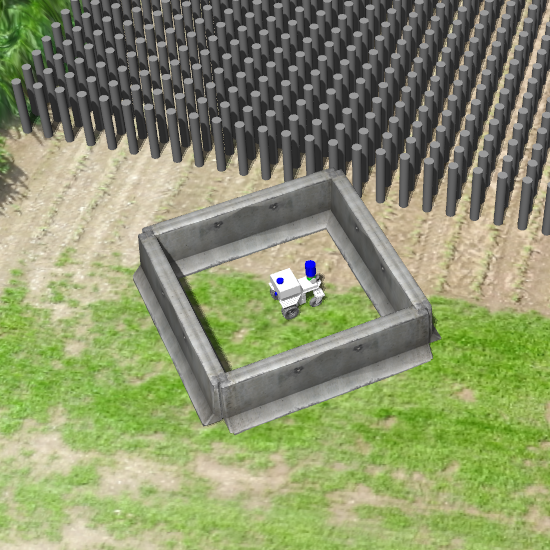
\includegraphics[width=0.3\textwidth]{pics/robot_prison.png}
    \caption{\textsc{\textquote{Robot Prison} - Static Obstacles that Completely Confine the Robot.}}
    \label{fig:robot_prison}
\end{figure}
Furthermore, the following (cf. fig. \ref{fig:obstacle_scenarios}) solvable static obstacle scenarios were implemented in order to test the robot's ability to overcome them. All of
these scenarios are predefined in the \code{ObstacleSpawner} configuration and can be arbitrarily spawned during a robot operation using the \code{/gazebo/spawn_sdf_model} service.
The number plate on the ground always indicates
the target position of the robot in the manual evaluation of the corresponding scenario. However, they also coincide with the general direction in which the robot must overcome them in
a simulated mission, i.e., the prototype scenario described in section \ref{sec:prototype_scenario}. The idea is essentially to block the robot's direct path and see whether it is
able to come up with an alternative. In this manner, the situation that a static obstacle appears on the robot's route can be simulated, and the robot is usually able to manage it.
\begin{figure}[H]
    \centering
    \begin{subfigure}[b]{0.24\textwidth}
        \centering
        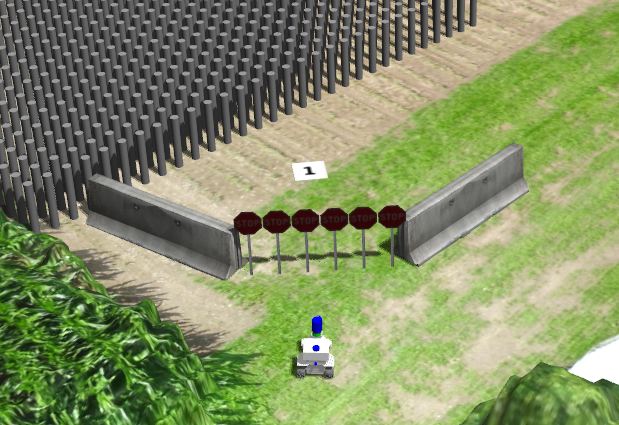
\includegraphics[width=\textwidth]{pics/static_1.png}
        \caption{\textsc{Scenario One}}
        \label{fig:static_1}
    \end{subfigure}
    \hfill
    \begin{subfigure}[b]{0.24\textwidth}
        \centering
        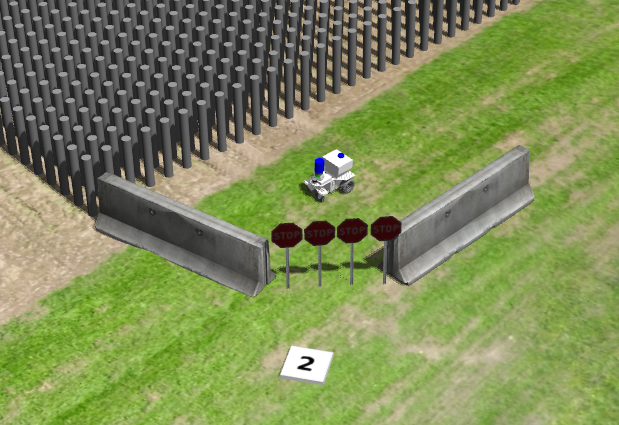
\includegraphics[width=\textwidth]{pics/static_2.png}
        \caption{\textsc{Scenario Two}}
        \label{fig:static_2}
    \end{subfigure}
    \begin{subfigure}[b]{0.24\textwidth}
        \centering
        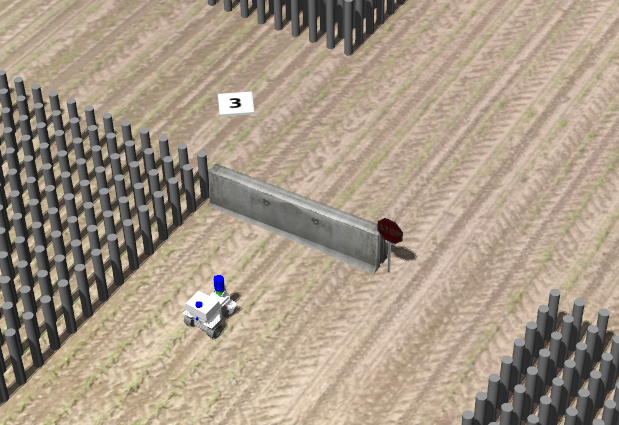
\includegraphics[width=\textwidth]{pics/static_3.png}
        \caption{\textsc{Scenario Three}}
        \label{fig:static_3}
    \end{subfigure}
    \hfill
    \begin{subfigure}[b]{0.24\textwidth}
        \centering
        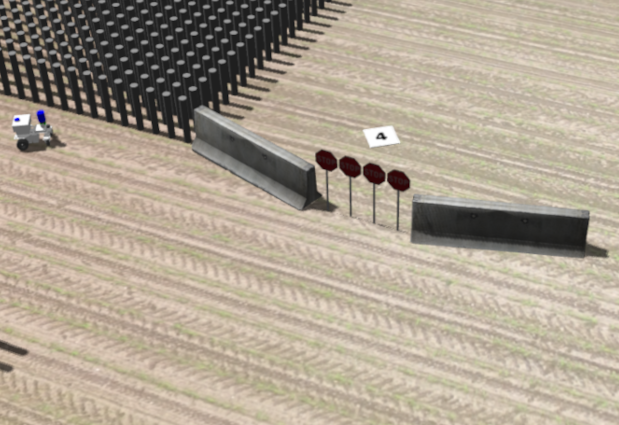
\includegraphics[width=\textwidth]{pics/static_4.png}
        \caption{\textsc{Scenario Four}}
        \label{fig:static_4}
    \end{subfigure}
\caption{\textsc{Solvable Static Obstacle Scenarios.}}
\label{fig:obstacle_scenarios}
\end{figure}
For instance, fig. \ref{fig:obstacle_success} shows how the robot copes with the first scenario (cf. fig. \ref{fig:static_1}). As can be seen, the robot manages to iteratively
progress around the static obstacle until it reaches the blocked target. This illustrates that unexpectedly appearing obstacles are not a great problem as long as there is a way.
Nevertheless, if they are, it will be detected by the aforementioned monitoring method.
\begin{figure}[H]
    \centering
    \begin{subfigure}[b]{0.24\textwidth}
        \centering
        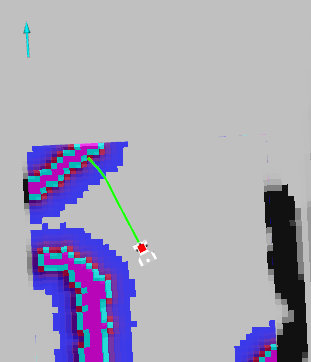
\includegraphics[width=\textwidth]{pics/succ_1.png}
        \caption{\textsc{}}
        \label{fig:succ_1}
    \end{subfigure}
    \hfill
    \begin{subfigure}[b]{0.24\textwidth}
        \centering
        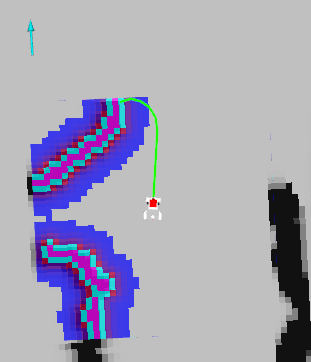
\includegraphics[width=\textwidth]{pics/succ_2.png}
        \caption{\textsc{}}
        \label{fig:succ_2}
    \end{subfigure}
    \begin{subfigure}[b]{0.24\textwidth}
        \centering
        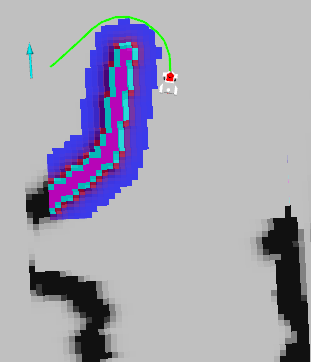
\includegraphics[width=\textwidth]{pics/succ_3.png}
        \caption{\textsc{}}
        \label{fig:succ_3}
    \end{subfigure}
    \hfill
    \begin{subfigure}[b]{0.24\textwidth}
        \centering
        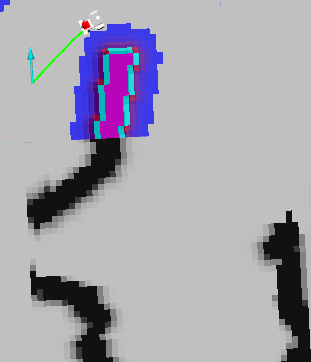
\includegraphics[width=\textwidth]{pics/succ_4.png}
        \caption{\textsc{}}
        \label{fig:succ_4}
    \end{subfigure}
\caption{\textsc{Successful Overcoming of Static Obstacle Scenario One.}}
\label{fig:obstacle_success}
\end{figure}
Unfortunately, it is not trivial to
simulate a case where \code{move_base_flex} fails on every attempt, although there is a path. Depending on the location and surroundings of the robot, it is sometimes able to find
the right way after a while. Yet, it is sufficient to show that such situations exist, as this is adequate justification for the need to address them. The straightforward approach to
simulate such situations works as follows. The user can specify a set of points, e.g., the one (red crosses) shown in fig. \ref{fig:outlier_points} in the scenario described in section \ref{sec:prototype_scenario}.
These points are not hard to reach per se, but should be quite difficult to reach from certain locations, e.g. because there are many obstacles in between.
When simulating such a situation, the point from the specified set of points farthest from the robot's current position is chosen, which does not guarantee navigation problems,
but is a fairly good heuristic. As the user is supposed to specify these points in latitude and longitude, the robot's position is taken from the GNSS estimate, i.e. \code{/fix}.
\begin{figure}[H]
    \centering
    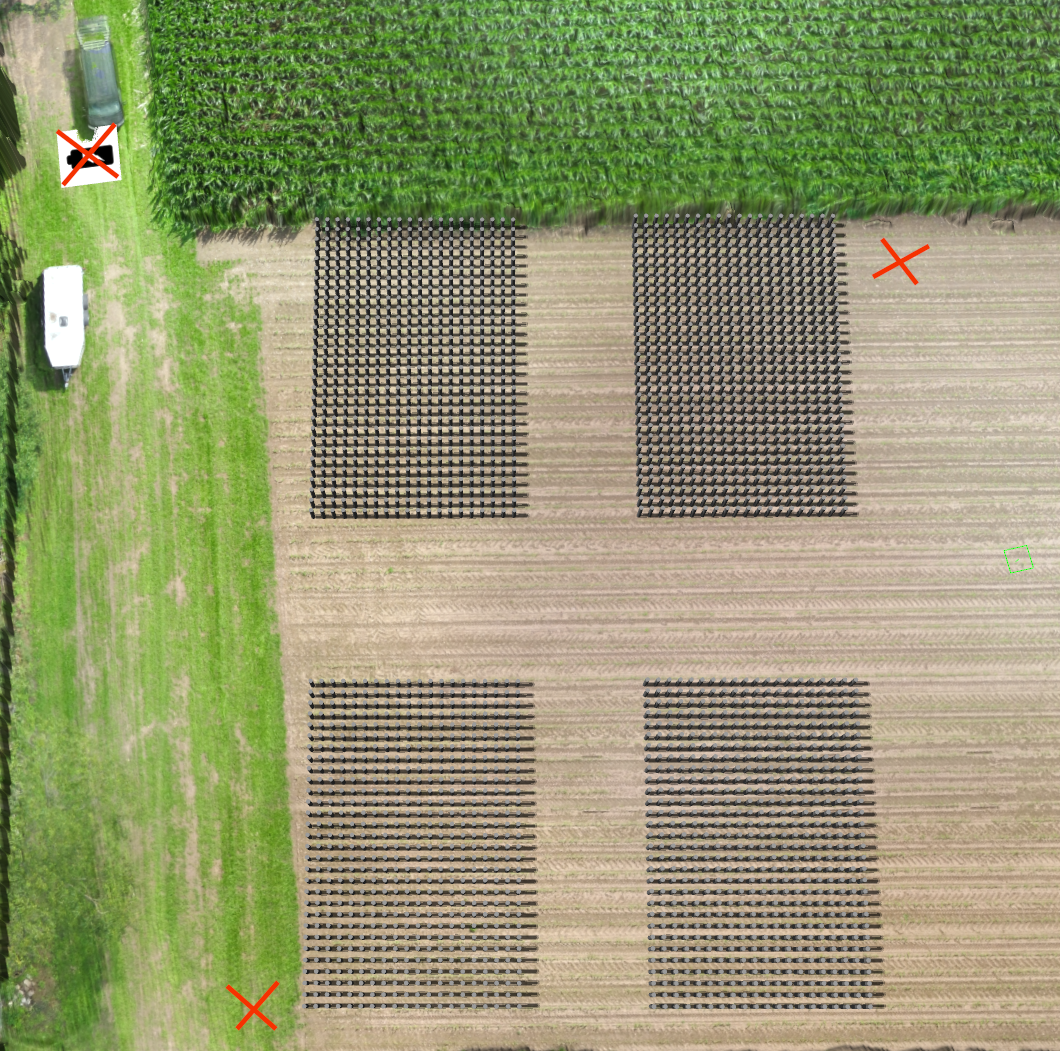
\includegraphics[width=0.3\textwidth]{pics/hard_to_reach.png}
    \caption{\textsc{Specified Set of \textquote{hard-to-reach} Points in the Prototype Scenario.}}
    \label{fig:outlier_points}
\end{figure}
As anticipated, this is not a guarantee of navigation failure, but it does cause it on a regular basis (cf. fig. \ref{fig:nav_fail}). It would be infeasible to simply interrupt the
active plan and set the selected point as navigation target, as there would then be no successful outcome that continues the plan. Thus, the dummy target is introduced as an
intermediate action in the plan, an option that is implemented as part of the low-level operation state machine. The \code{ObstacleSpawner} publishes the point to be used on
\code{/introduce_intermediate_nav_goal}, and the operation state machine executes it after the currently active action has been completed.
The simulation of the navigation failures can be enabled via the following ROS topics:
\begin{itemize}
    \item static obstacles \textrightarrow \code{/spawn_static_obstacles} with string message \code{`scene_n'}, $n \in \{1, 2, 3, 4\}$
    \item robot prison \textrightarrow \code{/spawn_robot_prison}
    \item navigation failure \textrightarrow \code{/trigger_nav_fail}
\end{itemize}
Navigation failures that are in principle solvable, i.e. not inescapable, can be addressed with the resolver described in section \ref{sec:nav_fail_resolver}.

\subsection{Incorrect or Inaccurate Localization}
\label{sec:sim_and_mon_incorrect_localization}

In general, localization is a complex topic whose detailed consideration is far beyond the scope of this work.
Nevertheless, it would be very valuable to develop a monitoring approach that is capable of realizing situations in which the localization is no
longer accurate, as there is a simple workaround that alleviates the problem in practice in many cases: Just driving the robot
a few meters back and forth to recalibrate the localization using different GNSS positions. The localization of the AROX system
is based on three components, IMU (inertial measurement unit), odometry and GNSS. Hence, incorrect or inaccurate localization can only be the product of problems in the pose
estimation of one or more of these components. There are numerous causes of drift and accumulated sensor errors, such as wheel slippage or being exposed to local magnetic fields
or magnetic materials. \cite{Bechar:2016} An implementation of a generalized
extended Kalman filter (cf. ROS community package \code{robot_localization}) is used to fuse the data from the different
sensors. The idea of a localization monitoring procedure is to measure the quality of localization. In absolute values, the
quality of localization cannot be determined. Of course, one could compare the used localization to another localization method,
i.e. to a redundant system. An example of such a redundant system could be a landmark localization where, for example, there are
fixed measured (known) reference points to which the robot can go to compare with its current localization. In the scenario
considered, however, such a system does not yet exist. Therefore, the plausibility of the localization can only be estimated
from the sensor data, which is retrievable via ROS topics (\code{/imu_data}, \code{/odom}, \code{/odometry/filtered_odom},
\code{/odometry/gps}). The messages arriving on these topics are of type \code{sensor_msgs/Imu.msg} and
\code{nav_msgs/Odometry.msg} respectively. The GNSS is perhaps the easiest component to monitor because at least the variance of the data is provided most of the times.
If the position estimates have a high variance, i.e. are not very reliable, it is probably not very accurate at the moment. GNSS monitoring is already part
of the connection monitoring described in section \ref{sec:sim_and_mon_gnss_connection_problems}. In contrast, IMU and odometry data are not as straightforward to
verify. One idea is to let the robot take known states and check if the values are what would be expected, e.g. let the robot
stand still and check whether the IMU values (angular velocity and linear acceleration) are approximately zero. Likewise, if no
control values are sent to the motors, the odometry values (twist) should be approximately zero. Since GNSS information cannot be
immediately compared to odometry data because the position is given in latitude and longitude, there is the \code{/odometry/gps}
topic where the GNSS information is converted to the same format as the odometry data, i.e. \code{Odometry.msg}. Moreover,
\code{/odometry/filtered_odom} is the result of sensor fusion of odometry and IMU data using \code{robot_localization}. Thus,
the difference between what arrives on \code{/odom} and \code{/odometry/filtered_odom} is due to the IMU. Unfortunately, it is
fairly common for IMU, GNSS, and odometry estimates to diverge considerably. That is why they are used in combination, their
weaknesses cancel each other out, which is why they complement each other well. As Khalastchi et al. put it: \textquote{\textit{When multiple sensors sense different aspects of
the (unknown) environment, their readings can be fused to form a consensus.}} \cite{Khalastchi:2018}
Odometry, for instance, is very good at continuously approximating the distance traveled,
i.e. the length of the trajectory, but is highly inaccurate when it comes to curves, which is why the trajectory can be in a completely wrong direction but with correct length.
A strength of GNSS, on the other hand, is the measurement / estimation of the absolute position. Yet, a single GNSS data point does not provide any orientation information at all.
As for the IMU, in principle one could try to use the linear acceleration (subtracting gravity) measured with the IMU to estimate the distance traveled by first integrating the
acceleration to get the velocity and subsequently integrating the velocity to obtain the displacement. Unfortunately, this process of double integration is numerically unstable
and becomes very inaccurate as even small sensor errors quickly explode. \cite{Yan:2018} As Yan et al. note, such an approach is not feasible unless one has access to an extremely
expensive military-grade IMU, which is generally not the case in field observation scenarios. Since the monitoring of the GNSS quality is already part of connection monitoring
(cf. section \ref{sec:sim_and_mon_gnss_connection_problems}), a high accuracy is assumed for this component of localization because if this were not the case, it would already have been detected by the corresponding connection
monitoring approaches. Consequently, if the connection monitoring does not report GNSS problems, it should be sufficiently accurate to be used to validate the other components,
i.e. IMU and odometry.\newline
There are monitoring approaches for the individual components of localization (IMU, odometry, GNSS) as well as those that compare two different localization components.
An example of the latter is the monitoring of the distance divergence between odometry and GNSS. It is sufficient to consider the two-dimensional distance, i.e. to use the $x$ and
$y$ coordinates of the current position estimate of the robot. Let $p_o$ be the current position estimate of odometry and $p_g$ that of GNSS. Of course, $p_o$ and $p_g$ can be
arbitrarily different, since odometry estimates the position relative to the robot's starting position, and GNSS estimates an absolute position on the Earth's surface, converted to
map coordinates. What should be approximately the same for both, however, is the distance traveled between the respective starting positions ($s_o, s_g$) and the latest positions
($p_o, p_g$) at all times. Therefore, one only needs to compare the Euclidean distances between the initial and latest positions for the odometry $d_o$ and for GNSS $d_g$,
i.e. $d_o = \sqrt{\sum_{i=1}^{n}(s_{o_i} - p_{o_i})^2}$ and $d_g = \sqrt{\sum_{i=1}^{n}(s_{g_i} - p_{g_i})^2}$. Now the divergence $|d_o - d_g|$ between the two estimates can be analyzed.
There are user-configurable divergence thresholds that trigger information via \code{/robot_info} or contingencies via \code{/contingency_preemption} based on severity. Significant
divergences may certainly be an indicator of localization problems. The usually more precise filtered odometry data is used for this purpose.
An extreme example leading to such a discrepancy would be a very poor GNSS link providing a highly inaccurate
position estimate that sort of teleports the robot away from its previous position, inducing the \textit{kidnapped robot problem}. Another monitoring approach that compares different
localization components is $yaw$ angle monitoring, arguably the most relevant kind of orientation for
ground vehicles. As mentioned above, GNSS itself does not provide any orientation at all. However, if it is known that the GNSS data is very accurate at the moment, it is feasible
to interpolate an orientation based on two successive GNSS positions $\hat{p}_g, \tilde{p}_g$, since it is evident that the direction in which the robot was moving was
$\overrightarrow{\hat{p}_g\tilde{p}_g}$ when the trajectory led from $\hat{p}_g$ to $\tilde{p}_g$. $\hat{p}_g$ and $\tilde{p}_g$ are taken from \code{/odometry/gps}, i.e. in map
coordinates. This estimated orientation can be compared to the orientation components of the
IMU and filtered odometry. Obviously, such an interpolation yields only the $z$ or $yaw$ component of the orientation. The idea is to always keep track of the latest $\tilde{p}_{g}$
and second latest $\hat{p}_{g}$ GNSS position estimates. If the Euclidean distance between the two exceeds a certain minimum interpolation threshold $i_{min}$, i.e.
$\sqrt{\sum_{i=1}^{n}(\hat{p}_{g_{i}} - \tilde{p}_{g_i})^2} > i_{min}$, the $yaw$ component is interpolated. The orientation vector
$o^{\top} = (\tilde{p}_{g}.x - \hat{p}_{g}.x \quad \tilde{p}_{g}.y - \hat{p}_{g}.y)$ is then used to calculate the angle $\arctan{\frac{o.y}{o.x}}$. After conversion to the format
suitable for comparison with \code{tf.transformations.quaternion_from_euler} the actual comparison can take place. Now it is again a matter of acceptable divergence, where the
user can specify a maximum feasible $yaw$ divergence $y_{max}$. When the absolute difference between the $yaw$ component of the IMU or filtered odometry orientation and the interpolated GNSS
$yaw$ component exceeds $y_{max}$, a contingency is initiated.
These were the monitoring approaches comparing different components of localization. The first monitoring for individual components considers the IMU. IMU monitoring is based on two
lists of IMU data. The first one stores active IMU data, meaning IMU data that has been recorded during \code{move_base_flex} activity, i.e. \code{GoalStatus.ACTIVE}.
Thus, the status of \code{move_base_flex} is taken into account at any time during localization monitoring. However, a certain generality is realized.  If other navigation
frameworks such as the basic \code{move_base} are present in different scenarios, they can also be used if they work with the common \code{actionlib_msgs}
\footnote{https://wiki.ros.org/actionlib\_msgs}. Additionally, since the transition between active and passive states in \code{move_base_flex} can be quite abrupt while smaller
movements are still taking place, there is a certain timeout between monitoring intervals after the mode change. For instance, when the robot moves to its next target,
\textquote{active monitoring} starts a few seconds after the mode change from passive to active. The same applies to the transition from active to passive. The second list
stores IMU data for inactive situations. It is important to note that IMU data is not gathered for all inactive states, but only for \code{GoalStatus.SUCCEEDED}. The other reasons
for inactivity, e.g. \code{GoalStatus.REJECTED}, are already accounted for at other levels of execution monitoring. In addition, unprocessed linear and angular twists would still be
part of the IMU data and would be added to the passive IMU history, distorting the results.
For both, due to the high frequency of $100Hz$ at which the IMU data arrives, as well as natural \textquote{anomalies}, a fairly long
history is tracked. The length of the history $n$ is user-configurable, the default is $n = 1500$. The first aspect monitored is the angular velocity for passive IMU data $a^p$ in
$rad/s$ measured by the IMU's gyroscope.
Since this is data recorded in the passive state, i.e. when the robot was not moving, it is expected that $a^p.x \approx a^p.y \approx a^p.z \approx 0 \thinspace rad/s$.
There is a user-defined upper bound $a^p_{max}$ for the angular velocity in the passive state. For all three directions, the average over the last $n$ absolute angular velocities in
the passive state is considered. If one of these values exceeds $a^p_{max}$, i.e. $\thinspace \exists \thinspace \frac{1}{n}\sum_{i=1}^{n} |a^p_i.d| > a^p_{max}, d \in \{x, y, z\}$, a contigency is initiated.
The next aspect is the linear acceleration in $m/s^2$ measured by the accelerometer of the IMU.
Both linear acceleration and angular velocity are examples of observations with contextual errors, where certain measurements (non-zero values) are legitimate in some
contexts but illegitimate in others, e.g. motion versus stasis. \cite{Khalastchi:2018} In preparation, a user-configurable fraction of the active and passive IMU
history is considered, sorted in descending order by the maximum absolute linear acceleration in the $x$ and $y$ directions for each IMU entry in the respective list.
For both, the median is taken to obtain a representative value ignoring outliers. To increase reliability, there are again histories with configurable length $m$ for these values.
In summary, these lists contain the median values of a certain fraction of the largest absolute linear acceleration values in $x$ and $y$ directions in the active and passive states.
Obvioulsy, the $z$ direction is not considered, since it always contains $g \approx 9.81m/s^2$. One could simply subtract $g$ and still take the direction into account, but it is not
as relevant as the others and is therefore disregarded. Then the average ratio between the two is calculated, i.e. for each value $l^p$ in the passive linear acceleration list and
each value $l^a$ in the active linear acceleration list the ratio $\frac{l^a}{l^p}$ is calculated. If the average of these ratios is below a user-defined minimum ratio $r_{min}$,
i.e. $\frac{1}{m} \sum_{i=1}^{m} \frac{l^a}{l^p} < r_{min}$, a contingency is initiated, as the linear acceleration during motion should be significantly higher compared to standstill.
Additionally, if one of the median values $l^p$ in the passive linear acceleration history exceeds an upper bound for linear acceleration $l_{max}$ at standstill, a contingency is initiated,
analogous to the case of too high angular velocities during inactivity. In the last step of IMU monitoring, the covariance matrices are checked. Each component, i.e. orientation, angular
velocity and linear acceleration, can have a covariance matrix $C_{3 \times 3}$ for the three axes $x, y, z$. As with GNSS covariance monitoring, only the standard deviations, i.e.
$\sqrt{c_{ii}} \thinspace \forall \thinspace c_{ii} \in C, i \in \{x, y, z\}$, will be considered. An upper limit $d_{max}$ for the standard deviations can be configured. Since these matrices are
not always provided or filled with meaningful entries, it must first be checked whether this is the case. If $c_{ij} = 0 \thinspace \forall \thinspace i, j \in \{x, y, z\}$,
it can be assumed that the covariance is unknown and it should be disregarded in monitoring. Moreover, if $c_{xx} = -1$, it means that the IMU device used does not support estimates
for this data, e.g. because the IMU in question does not provide an orientation estimate. If neither is the case, the standard deviations are monitored.  If any
of them exceeds the threshold, i.e. $\exists \thinspace \sqrt{c_{ii}} > d_{max}, i \in \{x, y, z\}$, a contingency is triggered due to a high IMU standard deviation. Finally, there is odometry monitoring, both for pure
odometry and filtered odometry with IMU data. The first point is again based on a known condition. When the robot is stationary, i.e. when \code{move_base_flex} has no active target,
all components of linear and angular twist should be approximately zero. An upper limit can be set for both. If one of the components exceeds this threshold in one direction, a
contingency is triggered due to an unexpectedly high twist in the passive state. Furthermore, there is pose and twist covariance monitoring. This time based on
covariance matrices $C_{6 \times 6}$ for the following list of components $\{x, y, z, roll, pitch, yaw\}$. Again, only the variances on the diagonal are considered. The pose uncertainty as well as the uncertainty of the velocity
in free space are checked for excessive standard deviations and initiate an interruption of the normal operation if necessary. In a nutshell, the general idea of localization
monitoring is to check expected values for known states. All localization monitoring is performed at a frequency specified by the user. To avoid timing issues during transitions from
active to passive states and vice versa, there is a short timeout that blocks monitoring immediately after a transition. A further aspect worth mentioning is that not all identified
issues that are monitored are actually erroneous localizations. When the robot is subjected to a certain forward acceleration even though it has no active navigation target, this is
not necessarily wrong, just unexpected. A slip on an icy surface that causes a position change without an active navigation target may be unexpected, but it is still true that the
position has changed. Nonetheless, this can cause problems with localization, since, for example, the odometry data no longer matches the GNSS data, which makes re-initialization of
the localization advisable. In order for a system to make use of the localization monitoring node, its localization must be based on sensor fusion of IMU, odometry, and GNSS data,
and it must provide the corresponding sensor information on the aforementioned topics. Additionally, it requires a navigation based on \code{actionlib_msgs/GoalStatus.msg}, e.g.
\code{move_base} or \code{move_base_flex}. Kinematics also play a role; in general, it should be a wheeled robot with differential drive. While an Ackermann drive would also be
permissible, others, such as omni-drive robots, are not compatible because they would violate certain assumptions used in the monitoring approaches, such as in the orientation
interpolation based on GNSS data.\newline

\noindent
As previously, the evaluation of localization problems as well as the corresponding monitoring procedures demands the simulation of such cases. For this purpose a
\code{PhysicsController} node was written. The general idea of the \code{PhysicsController} is to manipulate certain aspects of the physics in the \textit{Gazebo} simulation to
provoke the circumstances that lead to localization problems. The ROS services \code{/gazebo/pause_physics} and \code{/gazebo/unpause_physics} are used to pause and unpause the
simulation before and after physical manipulations, respectively. For the actual manipulation of physics, the \code{/gazebo/set_physics_properties} service is utilized. The most
important aspects of a physics property specification request are the gravity vector and the \code{ODEPhysics}\footnote{Open Dynamics Engine (https://www.ode.org/)} configuration,
i.e. the configuration of the physics engine used by default in \textit{Gazebo}. Initially, \code{ODEPhysics} is configured with reasonable default values from the literature and the
ODE documentation. The gravity vector $\vec{g}$ is naturally initialized with $\vec{g} = (0, 0, -9.81) \thinspace m/s^2$. The first simulation option is a wheel motion with no change
in position, resulting in a distance divergence between the estimated distances traveled by odometry and GNSS. In practice, such a situation can for example occur when the wheels spin
due to low friction on an icy or muddy surface. First, the gravity, i.e. acceleration in $z$ direction, is set to a low positive value for a short time to levitate the robot above
the ground, e.g. $\vec{g} = (0, 0, 0.4) \thinspace m/s^2$. To prevent flying off, a small negative acceleration is then briefly set in the $z$ direction. Finally, the robot should
hover in this position for a certain time so that the wheels can rotate without touching the ground, i.e. changing the position of the robot. For this purpose, the acceleration in
all directions is set to $0 \thinspace m/s^2$. After a short period of time, normal gravity is restored, i.e. $\vec{g} = (0, 0, -9.81) \thinspace m/s^2$. The second simulation option
is the reverse case - a change in position without wheel revolutions, which in practice could be related to the robot slipping away on a muddy path. This can be simulated by briefly
changing the acceleration in $x$- or $y$-direction to a relatively high value (e.g. $8 m/s^2$) so that the robot drifts off. 
The third option, a divergence between the estimated yaw angles of the interpolated GNSS positions, the filtered odometry and the IMU, can be simulated by rotating the robot by e.g.
$50\degree$ around the yaw axis. This assumes knowledge of the robot's current pose (position + orientation). The position is taken from \code{NavSatFix} messages to the \code{/fix}
topic, and the angular rotation, i.e. orientation, based on the IMU's gyroscope is extracted from the latest \code{Imu} message to \code{/imu_data}.
The pose is always kept available in terms of latitude ($lat$), longitude ($lng$), and the yaw angle $yaw$ in degrees. Since the IMU stores
the orientation as a quaternion, the function \code{tf.transformations.euler_from_quaternion} is used to obtain the Euler angles $roll, pitch, yaw$. Eventually,
$yaw = yaw \cdot \frac{180}{\pi}$ to convert the resulting radians to degrees. For the actual simulation, $yaw$ is increased by $50\degree$ if it does not exceed $180\degree$,
since $yaw \in [-180\degree, 180\degree]$. Otherwise, $yaw = -180 + ((yaw + 50) \mod 180)$. This adjusted $yaw$ angle is the goal orientation. A \code{Twist.msg} is created,
which then accounts for the actual rotation by being published to \code{/cmd_vel}. Since the rotation is supposed to distort the active \code{move_base_flex} navigation, it must
be published at a very high frequency as long as the actual rotation of the robot is approximately equal to the defined target angle $yaw$. The tolerance is configurable by the user.
To further amplify the impact on the active navigation, the twist publishing is accompanied by some gravitational changes, a positive low gravity in $z$ direction (e.g. $0.2$) and
a slightly stronger acceleration in the $x$ and $y$ directions (e.g. $2.5$). This gravitational change does not start immediately, but only after a configurable number of twist
messages have been published on \code{/cmd_vel}, resulting in a reinforced rotational distortion. The value of the angular twist in $z$ direction is $\pi$ or $-\pi$, depending on
the initial orientation. After the target $yaw$ is reached with sufficient accuracy, normal gravity is restored. A real-world problem reproduced by this simulation is when the robot
unexpectedly slips away and turns during navigation.
Furthermore, the situation of too high acceleration values detected by the IMU's accelerometer can be simulated in situations
where the robot is supposed to stand still. For this it suffices to apply a rather low acceleration in $x$- or $y$-direction for a brief period of time. Additionally, an unexpected
motion for the odometry can be simulated by publishing a linear twist (change to be performed) on \code{/cmd_vel} to let the robot move slightly without active navigation goals.
Practically, both cases may refer to situations where the
robot does not have an active navigation goal, but is moved for some reason, e.g. slipping away. Crucially, not all of the simulated processes described can take place at all times.
Therefore, the status of \code{move_base_flex} must be taken into account by subscribing to \code{/move_base_flex/exe_path/status}. Whenever a simulated localization error is
triggered, a flag is set, but actual execution is not initiated until the required \code{move_base_flex} state is encountered. For instance, the simulated case of wheel revolutions
without position change can only be performed if there is an active navigation target causing the wheel revolutions. Thus, when the most recent status of \code{move_base_flex}
changes from a passive state to \code{GoalStatus.ACTIVE}, the simulation is initiated. To ensure the distance divergence, there is also a high-frequency linear twist published to
\code{/cmd_vel}, which amplifies the wheel rotations. Likewise, the case of a change of position without wheel revolutions should take place in a
passive state. A particular challenge is the simulation of deviations in yaw angle estimation. First, they can only be simulated in \code{GoalStatus.ACTIVE}, as the corresponding
monitoring is disabled in passive states, due to the fact that a divergence in yaw angle estimates in passive states can only result from unexpected movements in passive states,
which is already covered by other monitoring options. If the yaw estimates diverged in the passive state without a change in position, the divergence would have already been present
in the active state that led the robot there, and should thus be detected in the active state. In addition, there could be cases where active navigation ends with a rotation on the
spot to align the robot in an expected orientation, which would always cause a contingency of this type after the transition to the passive state, since the GNSS interpolation is
inevitably obsolete after the rotation. Consequently, monitoring and simulating yaw divergence is only meaningful during active navigation. Beyond that, of course, there can be no
GNSS interpolation in the passive state, because the position of the robot does not change by definition and thus there can be no two distinct positions. Aside from the fact that
rotating on the spot is a frequent occurrence in standard navigation, this is a common recovery behavior that should certainly be viable. For this reason, the aforementioned
interpolation threshold $i_{min}$ was introduced, since otherwise a rotation on the spot would always trigger a yaw divergence. That is why it is not sufficient to simulate a
rotation on the spot, there must also be a minor change in position that does not precisely match the robot's orientation. Simultaneously, this motion cannot be too large, otherwise
a case of distance divergence would be triggered. It takes some experimentation to find a stable configuration for the system in question, but the idea should be clear.
It is also worth mentioning that the simulations are not necessarily sharply separated. For instance, applying a force to trigger high acceleration values recorded by the IMU may
very well cause wheel rotations, triggering other problem cases such as estimated position changes by the odometry. Conversely, letting the wheels rotate will accelerate the robot
and result in higher IMU values. Finally, the two remaining simulation cases of motion in passive states indicated by IMU and odometry can obviously only be simualted when no
active navigation goal is being pursued, otherwise the motion would be expected. The simulation of the localization failures can be enabled / disabled via the following ROS topics:
\begin{itemize}
    \item \textbf{odometry-GNSS distance divergence (type $1$)} \textrightarrow \code{/wheel_movement_without_pos_change}
    \item \textbf{odometry-GNSS distance divergence (type $2$)} \textrightarrow \code{/pos_change_without_wheel_movement}
    \item \textbf{interpolated GNSS and IMU/odometry yaw divergence} \textrightarrow \code{/yaw_divergence}
    \item \textbf{IMU acceleration, although no active navigation target}\newline \textrightarrow \code{/moving_although_standing_still_imu}
    \item \textbf{odometry twist, although no active navigation target}\newline \textrightarrow \code{/moving_although_standing_still_odom}
\end{itemize}
\noindent
Localization-related challenges for LTA can be addressed using the resolver described in section \ref{sec:localization_resolver}.

\section{Solutions for LTA Challenges}
\label{sec:solutions_for_lta_challenges}

As anticipated, the focus of this work is on detection, and an initial solution adopted for all the issues identified in section \ref{sec:challenges_for_lta} is to communicate the
problem to a human operator. However, as can be concluded from section \ref{sec:sim_and_mon_of_lta_challenges}, there is only one identified problem that explicitly causes a
catastrophe condition and thus relies on the fallback option of requesting the help of the human operator.
This problem is the power management failure, where it is determined that the robot is definitely no longer able to reach the base station to recharge its
battery. This is the only case where the robot is definitely no longer able to solve the problem and immediately calls the operator for help. All other problems start with a
contingency and therefore launch at least a simple heuristic or workaround that attempts to resolve the issue before transitioning to the catastrophe state in case  all other solution
attempts are unsuccessful. Surprisingly, workarounds often lead to success, sometimes very simple approaches are sufficient, such as waiting for a short time, restarting a component,
changing the position slightly, etc.
In general, the idea of recovery is to transform an erroneous or problematic state into one without any issues. \cite{Brodskiy:2011}
The idea is to have the monitoring procedures described in section \ref{sec:sim_and_mon_of_lta_challenges} that
look for the specific types of issues and initiate an appropriate response. Kunz et al. \cite{Kunz:2009} emphasize that the robustness of a system can be maximized by
providing fail-safe procedures. Although they are dealing with AUVs, the general problem remains the same.\newline
Whenever a monitoring solution described in section \ref{sec:sim_and_mon_of_lta_challenges} causes a transition to the \code{CONTINGENCY} or \code{CATASTROPHE} states
by publishing on the respective topics \code{contigency_preemption} or \code{catastrophe_preemption}, information about the cause of the interruption is
transmitted via a ROS message. Based on this cause, the corresponding resolver class is selected and executed. The idea is that each general problem class, e.g.
connection problems, provides a resolution method for each potential specific problem in that class, e.g. poor WiFi link quality. The \code{CONTINGENCY} state in turn
communicates the failure reason to the resolver classes. If available, the specific resolving method will be executed. Afterwards, the outcome is reported back to the
high-level state machine, which either continues normal operation if the problem is successfully solved, or aggravates to catastrophe. To this end, each monitoring node publishes on
a topic \code{/aggravate}, which then initiates the transition from \code{CONTINGENCY} to \code{CATASTROPHE}. Thus, if the specific resolver
method is not able to handle the problem, or if there is not even a specific resolver method for the failure case, the problem is handed over to the fallback resolver,
which passes the problem to the human operator and awaits resolution. If the respective failure was caused by a simulation, the corresponding flag must be reset to restore
normal operation, which is done by publishing on the particular toggle topic described in section \ref{sec:sim_and_mon_of_lta_challenges}.

\subsection{Fallback Solution - Requesting Help of a Human Operator}
\label{sec:fallback_solution}

Requesting assistance from a human operator was identified early on as a crucial aspect of long-term autonomous mobile robots: \textquote{\textit{[...] critical aspect of autonomy in our
unsupervised application is the ability to detect failure and signal humans for help}}. \cite{Nourbakhsh:2003}
Communication with a human operator, i.e. notifying a human operator that a problem has occurred that requires human intervention or providing useful information about the state
of the robot or mission, is implemented as a separate \code{OperatorCommunication} class. The robot-human communication module is subscribed to two different topics. First, a message
on \code{/request_help} indicates that the robot is requesting the help of a human operator, i.e., is unable to solve a problem by itself. The second topic is \code{/robot_info},
which is used for minor problems or tasks that do not require immediate action, but are good to know and tackle soon, e.g. a memory usage of $90\%$. According to the definitions in
section \ref{sec:plan_execution_and_monitoring}, a request for assistance to the human operator is always triggered by a catastrophe situation. This means that the human operator is
notified and the robot then performs a graceful shutdown. Therefore, the robot aborts its current mission and cannot restart or continue until the problem is solved by the human
operator and the robot is restarted. All the monitoring modules described in section \ref{sec:sim_and_mon_of_lta_challenges} are subscribed to the \code{/robot_info} topic and thus
able to communicate relevant information. The more critical topic for catastrophe cases can be triggered directly by the power management monitoring node and additionally as a result
of a failed resolution attempt by the resolver methods described in the following sections.

\subsection{Power Management}
\label{sec:power_management_resolver}

Of the two types of power management faults considered (cf. section \ref{sec:sim_and_mon_power_management}), one can be solved by the robot autonomously, namely the case in which it
must immediately return to the charging station to prevent a total failure. The solution to this problem is based on the introduction of two intermediate goals into the plan
- \code{return_to_base} and \code{charge}. For this purpose, the operation state machine provides the topic \code{/introduce_intermediate_recharge_goal}. Messages on this topic
cause these two actions to be inserted at the front of the plan, i.e. as the next actions to be executed. Compared to implementing the return to base and recharge procedure as part of
the resolution, this method of augmenting the plan and returning to normal operation has the distinct advantage of having all monitoring procedures active again and allowing for any
necessary handling of other contingencies, such as docking or charging failures. Generally, this plan modification and subsequent continuation of normal operations is much more elegant.
This kind of plan augmentation is a very classical problem that entails many subtleties and, in general, is not trivially solvable. However, in the context of this work, this is
possible based on the management of such situations described in section \ref{sec:plan_interruption_section}. The other type of failure, i.e., a catastrophe, as defined in this
thesis, is not solvable by the robot itself. The resolver node reports the problem to the human operator and initiates a graceful shutdown of the robot.

\subsection{Charging Failure}
\label{sec:charging_failure_resolver}

There are plenty of cases where the robot can remedy charging faults on its own. Docking failures, regardless of whether they are due to detection or navigation problems, are tackled
in the same simple and often effective way: Simply repeating the \code{return_to_base} action. Obviously, this solves the problem of an unsuitable destination. However, it
furthermore often solves problems with detection, as a slight change in position often realigns the perspective on the container, which can be helpful. This autonomous resolution is
performed only once. There is a counter, and if one docking failure is followed by another, it is not worth trying repeatedly, but to notify the human operator immediately. This
covers all cases where the robot is not able to solve the problem, e.g. if the ramp is raised and the robot cannot drive in. Since the natural solution that a human would perform in
such a case would be to lower the ramp and thus open the container, this is what is done in this case, in a sense as a predefined reaction of a human operator. For this purpose, a
value of $j = \frac{\pi}{2}$ is sent to \code{/container/ramp_position_controller/command} (cf. section \ref{sec:sim_and_mon_charging_failures}). In principle, it would also be
reasonable to equip the robot with a resolution function for lowering the ramp, but the real version of the container in the considered scenario does not yet provide automated ramp
lowering. Additionally, the local and global costmaps are cleared so that the robot can immediately perceive the open container. The clearing of costmaps is already described in
detail in section \ref{sec:nav_fail_resolver}. The resolution of undocking failures is based on the premise that they are often due to slightly inappropriate positioning of the robot.
Hence, the resolver moves it back and forth a bit by publishing linear twists to \code{/cmd_vel}, which practically solves the problem in some cases. As in the case of docking
failure, this is attempted only once. If the robot still fails to undock, the human operator is notified, including a potential lowering of the ramp and clearing of the costmaps
if necessary. Eventually, to the third type of charging failure, i.e. the explicit non-functioning of the battery charging, despite successful docking. As this is often due to
imprecise alignment in front of the inductive charging plate, it may help to repeat the alignment process. Again, this resolution is performed only once. If it still fails, it
may be a more complex problem beyond the robot's ability to solve, which is why the operator is notified. All resolution counters that ensure that the respective method is only
attempted once are reset at appropriate events. The counters for docking and charging failure resolution are reset when the battery charge level increases after the docking
error, as this is a clear indicator that the docking was finally successful and the battery is being charged. For this purpose the current state of charge is stored at the start of
the docking resolution and later compared with the most recent state on \code{/arox/battery_param}. The undocking resolution count is reset when \code{move_base_flex} reports
\code{GoalStatus.SUCCEEDED}.

\subsection{Drastic Weather Change}
\label{sec:weather_resolver}

The resolver, which is launched after normal operation is interrupted when somewhat extreme weather conditions are detected by the monitoring procedures described in section
\ref{sec:sim_and_mon_drastic_weather}, operates as follows. All contingencies based on extreme weather events are resolved in the same manner: The robot returns to its base,
i.e. the mobile container, and seeks shelter. Thus, a \code{move_base_flex} navigation goal with the coordinates of the base station is executed. If successful, the robot
should charge its battery while waiting for moderate weather, i.e. it will be docked to the charging station in the base and start charging. When the battery is fully charged,
the robot waits for clearance before continuing its mission. If something goes wrong during this resolution attempt, e.g. the \code{move_base_flex} navigation fails, the
fallback solution of calling the operator for help is executed (cf. sec. \ref{sec:fallback_solution}). Clearance is transmitted via a topic \code{/moderate_weather} to which the
resolver subscribes to and on which the weather monitoring node publishes. After a contingency, the weather monitor transitions to a kind of passive monitoring where it no longer
initiates contingencies etc., but just passively observes the weather and estimates whether it has returned to moderate. If this is the case, it notifies the resolution procedure,
which then reports back successful resolution, and the high-level state machine can resume plan execution in normal operation mode. Finally, the weather monitoring node switches
back to active monitoring. In summary, the robot seeks shelter in extreme weather situations, uses the time to recharge its battery, and waits until conditions are moderate before
continuing to execute the plan.

\subsection{Sensor (Perception) Failure}
\label{sec:sensor_failure_resolver}

The solution approaches for sensor (perception) failures are rather trivial. There is once again a counter for resolution attempts. If it is the first sensor failure, the scan is
simply repeated. However, if it fails repeatedly, a catastrophe condition is initiated, i.e. the operator is notified and the system is shut down. The counter is reset at appropriate
times, e.g. when the scan was successful.

\subsection{Lost Connection}
\label{sec:connection_resolver}

Dealing with WiFi and GNSS connectivity issues is once again based on retries, counting them, and potential aggravation. The rationale is to have a short timeout, followed by a
reconnection attempt and notification of the problem in the event of a repeated failure. Internet connection issues, however, are resolved by
reinitializing the internet monitoring node, as this could fix a failed connection to the \code{speedtest} API. Of course, this is also not done arbitrarily often and in case of
repeated failure, the human operator is notified.

\subsection{Data Management}
\label{sec:data_management_resolver}

Data management problems are a special case as there is one case where the robot is definitely not able to solve the problem itself, namely the case of a full memory. However, this is
not a problem in principle. For instance, the robot could upload the scans instead of storing them on its drive, but for the prototypical scenario considered in this work, the robot
will store the scans on its drive, so this is a problem that must be solved by the human operator. Nevertheless, it is not a direct catastrophe case like the power management problem
where the robot cannot return to the base station due to its battery charge, but there is a useful step that can be taken before the catastrophe case is initiated. The robot can
return to its base and seek shelter before waiting for the human operator to take care of the problem. The second type of data management problem, i.e. an improperly logged scan, is
again addressed by a retry and count-based attempt before a catastrophe is triggered if necessary.

\subsection{Plan Deployment Failure}
\label{sec:plan_deployment_resolver}

All three of the plan deployment problems presented in section \ref{sec:sim_and_mon_plan_deployment_failures} can be addressed with workarounds that the robot can try
on its own, ignoring the fourth issue that only causes a message on \code{/robot_info} and no contingency case. The cases of empty or otherwise infeasible plans can be resolved
in some cases simply by requesting the plan again. For this purpose, the resolver keeps track of plan retrieval attempts. If the counter for either case is $0$, which means that the
first attempt to retrieve a plan failed, the resolution is to re-try and the counter is incremented. However, if the counter reaches a configurable threshold, e.g. $2$, which means
that the robot has already unsuccessfully requested the plan three times, it stops repeating the plan request, resets the counter and forwards the problem to the fallback solution,
i.e. it notifies the operator. In such a case, it should waste no further time and immediately notify the operator. The remaining problem case of an unavailable plan service can also
be dealt with by the robot itself in some cases. For this purpose, the plan generation node provides a topic \code{/activate_plan_service} that enables external service activation.
Thus, in case of an unavailable service failure, the resolver simply publishes on this topic and initiates a re-initialization of the plan generation service. Similar to the two
cases above, such a re-initialization is not performed arbitrarily often, but there is a counter and a limit that cause the problem to be forwarded to the human operator in case of
repeated failure. In summary, for all potential contingencies arising from problems in the deployment of the plan, the robot has a strategy to solve them itself. As always, when it
fails, it passes the problem on to the human operator.

\subsection{Navigation Failure}
\label{sec:nav_fail_resolver}

Irrespective of whether the navigation failure is due to a sustained recovery or an explicit \code{move_base_flex} error, the resolution is the same. Initially, both the global
and local costmaps are cleared to remove previous obstacles that are no longer present.
The order is crucial - first, the global costmap is cleared using the \code{move_base_flex/clear_costmaps} service. Subsequently, the local costmap
is cleared, which is implemented as a \code{move_base_flex} recovery, i.e. a \code{SimpleActionClient(move_base_flex/recovery, RecoveryAction)} is created and a \code{`clear_costmap'} goal is sent.
In case the global costmap is not cleared first, the obstacles in the global map are immediately copied back to the local map. Eventually, a simple but often effective workaround is
executed: Driving the robot to one of several specified recovery points. Since these points are mission-specific and set by the user with the intention of being easily accessible from
almost any location possible in the scenario, it often frees the robot from deadlocked situations and allows the mission to continue from there. The underlying idea is essentially to
consider the problem from a different perspective, i.e. to try to plan a path from the new position. Obvioulsy, it is not possible to solve inescapable
situations such as the \textquote{robot prison} from section \ref{sec:sim_and_mon_navigation_failures} in this way. Therefore, it is a necessity to continue monitoring the execution
of this navigation target as well. Both explicitly, i.e., the return of \code{move_base_flex}, and implicitly, i.e., sustained recoveries. The explicit case is trivial, it is a
simple check for \code{GoalStatus.ABORTED} cases directly in the resolution method. The implicit case, though, must again be determined by the monitoring procedure, which counts
failed recovery procedures (cf. section \ref{sec:sim_and_mon_navigation_failures}). For this purpose, the navigation monitoring node described in section
\ref{sec:sim_and_mon_navigation_failures} has another mode that is activated after navigation recovery is initiated. In this mode, recovery operations are counted again, but no
contingencies are triggered as in default active monitoring, instead a special topic \code{/resolution_failure} is used to notify the recovery procedure, which then cancels all
active resolution goals. For both types of errors during navigation failure recovery, human operator notification is initiated as a fallback solution. An additional aspect of
navigation error recovery that is essential for cases of simulated navigation failures is the removal of simulated obstacles. When the human operator intervenes in the event that
the robot is unable to cope with obstacles, it is expected that the operator will remove the obstacles before re-initiating the autonomous operation of the robot. Thus, an obstacle
removal function is implemented as part of the navigation failure monitoring node described in section \ref{sec:sim_and_mon_navigation_failures}. The most obvious example is the
\textquote{robot prison}, which must be removed as part of the resolution, otherwise the robot will not be able to continue its mission in the simulation. The \code{ObstacleSpawner}
keeps track of all spawned obstacle models. If a resolution was successful, obstacle removal is initiated via a topic \code{/clear_spawned_obstacles}, which causes the
\code{ObstacleSpawner} to despawn all models via the \code{gazebo/delete_model} service. Finally, after successful resolution, the active monitoring mode is reactivated via a topic.

\subsection{Incorrect or Inaccurate Localization}
\label{sec:localization_resolver}

The approach to resolving localization problems described below is not a panacea, but merely a workaround that can, however, help in many practical situations. Whenever the robot's
normal operation is interrupted due to localization issues detected by the monitoring procedures described in section \ref{sec:sim_and_mon_incorrect_localization}, the same resolution
approach is initiated: The robot is moved back and forth a few meters to recalibrate the localization using different GNSS positions. This is realized by publishing appropriate linear
twists to the \code{/cmd_vel} topic. Afterwards, the localization monitoring node is reinitialized, clearing all previously collected data, etc. Furthermore, the local costmap is
cleared to remove potential mapping anomalies resulting from the localization failure. This is achieved by sending a \code{clear_costmap} \code{RecoveryGoal} to the
\code{SimpleActionServer} for recoveries provided by \code{move_base_flex} as well as plain \code{move_base}. As usual, if something goes wrong during the resolution attempt,
the fallback solution of asking the operator for help is executed (cf. section \ref{sec:fallback_solution}).

\chapter{Integrated Solutions}
\label{sec:integrated_solutions}

In general, an integrative work benefits from many integrated solutions. Nevertheless, it should be viable in the scope of the work and robust. Essentially, there is a tradeoff
between integrating as much as possible, thereby increasing the functionality, and staying feasible and realistic. Two solutions developed in the course of the PORTAL project that
match very well with the framework proposed in this thesis are introduced in the following sections. Section \ref{sec:battery_monitoring} is concerned with a battery monitoring
solution, and section \ref{sec:docking_solution} presents a system that enables autonomous energy supply.

\section{Battery Monitoring}
\label{sec:battery_monitoring}

One solution worth integrating is a watchdog module developed as part of the PORTAL project that monitors the battery state and acts as a fail-safe. In principle, the charge stops are part of the plan, i.e. are
considered at planning time. Thus, there is resource planning for the missions that includes to be back at the base station before the robot runs out of battery. However, if it fails,
there should be a monitoring process at execution time that is able to react to wrong plans, i.e. the battery is depleted before expected and the robot has to return to its base.
The module essentially checks the distance from the robot's current position to the base station, the expected battery consumption to get there, and the remaining battery charge.
The base station essentially restricts the robot's radius of motion; the robot is, as Egerstedt et al. put it, \textquote{spatially anchored}. \cite{Egerstedt:2018} In summary, the
module is running at execution time, it does not schedule the charge stops in advance, but only responds to failure cases where the robot needs to preempt the plan execution, return
to its base and recharge. This battery watchdog is the basis for the power management failure monitoring presented in section \ref{sec:sim_and_mon_power_management}. In order for the
module to provide reasonable estimates, it is critical that the robot constantly reports its current mode of operation. The battery watchdog distinguishes between \code{scanning},
\code{traversing}, \code{waiting}, \code{docking}, \code{undocking}, \code{charging}, \code{dead}, \code{contingency} and \code{catastrophe}. All these modes are set in the operation
state machine (cf. section \ref{sec:execution_monitoring_smach_architecture}) at appropriate transitions by publishing to \code{arox/ongoing_operation}.

\vfill
\pagebreak

\section{Autonomous Energy Supply}
\label{sec:docking_solution}

A fundamental step towards long-term autonomy of a mobile robot is to ensure its power supply. Arvin et al. \cite{Arvin:2009} identify autonomous navigation and precise docking at
a charging station as major problems for mobile robots, since most mobile robots require human assistance to charge. They identify three critical aspects for mobile robots that can
recharge themselves: Awareness of the need to charge, locating and navigating to the charging station, and precise docking. For this purpose, there is an inductive charging station
located in a mobile container on the field site. For the PORTAL project, the container providing the inductive charging station was modeled in URDF and can be used in the \textit{Gazebo} simulation (cf.
fig. \ref{fig:container_model}).
\begin{figure}[H]
    \centering
    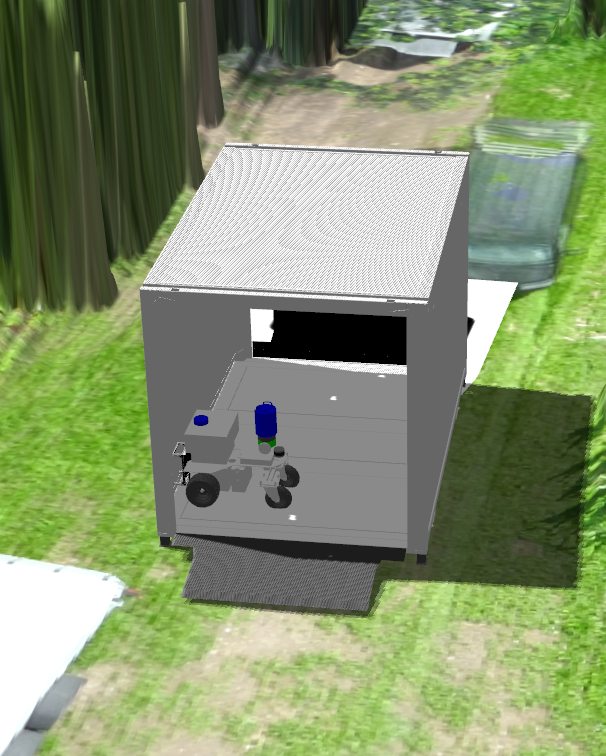
\includegraphics[width=0.3\textwidth]{pics/docked.png}
    \caption{\textsc{Robot Docked to Charging Station}}
    \label{fig:container_model}
\end{figure}
Thus, the power supply could be realized by integrating an autonomous docking / undocking solution that enables the robot to detect the container in a laser scan of its nearby
surroundings, drive into it and dock to the inductive charging station. Such a docking solution has been created as part of the PORTAL project and extended in this work by some
error handling mechanisms to realize meaningful monitoring. The docking solution is integrated into the framework developed in this thesis to provide the robot with autonomous
recharging capability. The part where the (un-)docking solution is integrated into the presented framework is
the operation state machine, which is responsible for the action execution (cf. section \ref{sec:execution_monitoring_smach_architecture}). Essentially, two of the available actions are extended: \code{return_to_base} and \code{charge}. First,
\code{return_to_base} must select the correct base pose specified by the user, i.e. the position to which it is supposed to move before charging its battery. In the case of the
simplified charging patch scenario, it is expected to be exactly on the patch. In the more realistic container scenario, however, it is assumed to be somewhere in the proximity of the
container and pointing approximately in its direction. In either case, the robot then drives to the specified location. Afterwards, the action is completed in the simplified charging
patch scenario. Yet, in the container scenario, \code{return_to_base} includes docking. Thus, docking is initiated by creating a
\code{SimpleActionClient(`dock_to_charging_station', DockAction)}. After sending the docking goal via this action client, the docking state machine visualized in fig.
\ref{fig:docking_smach} is executed.
\begin{figure}[H]
    \centering
    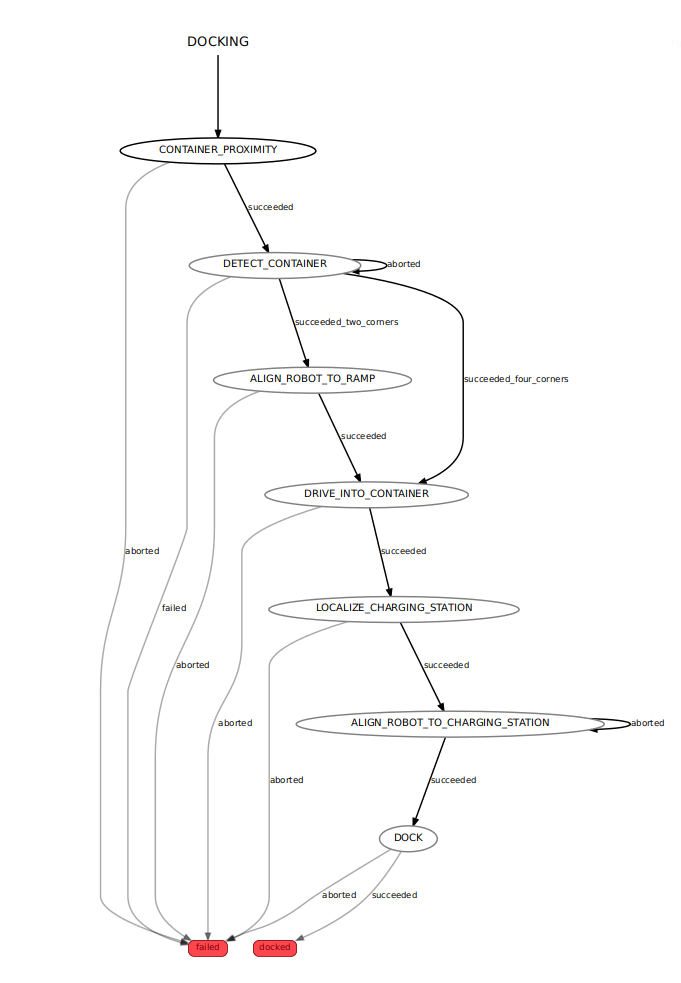
\includegraphics[width=0.75\textwidth]{pics/docking_smach.png}
    \caption{\textsc{Docking State Machine}}
    \label{fig:docking_smach}
\end{figure}
The first state is \code{CONTAINER_PROXIMITY}, which assumes that the robot has navigated close to the container, e.g. based on GNSS (cf. fig. \ref{fig:container_view}).
Subsequently, if this is the case, \code{DETECT_CONTAINER} begins based on a laser scan recorded by the robot facing the container. In simple terms, it performs a Hough transform
to detect lines in the scan and uses a large number of tailored rules to find a reasonable combination of line segments that could represent the container. Essentially, the whole
approach is centered around the idea that the container is a relatively simple geometric shape that can be detected in a laser scan - a combination of line segments
(cf. fig. \ref{fig:rviz_view}).
\begin{figure}[H]
    \centering
    \begin{subfigure}[b]{0.49\textwidth}
        \centering
        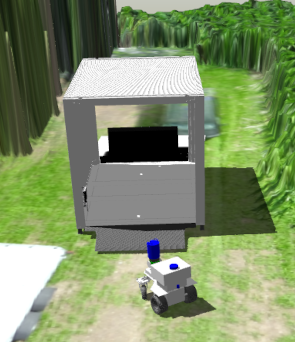
\includegraphics[width=0.5\textwidth]{pics/container_view.png}
        \caption{\textsc{Robot Facing the Container}}
        \label{fig:container_view}
    \end{subfigure}
    \hfill
    \begin{subfigure}[b]{0.49\textwidth}
        \centering
        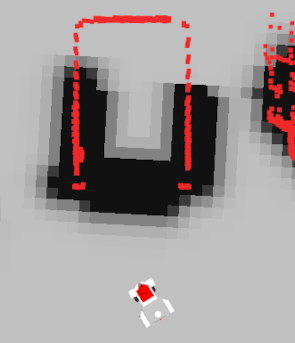
\includegraphics[width=0.5\textwidth]{pics/rviz_view.png}
        \caption{\textsc{Container Perception Based on Lidar}}
        \label{fig:rviz_view}
    \end{subfigure}
\caption{\textsc{Container Perception - Geometric Shape}}
\label{fig:container_geometric_shape}
\end{figure}
Initially, the input \code{LaserScan} in which the container is to be detected is transformed into the parameter space constructed by spanning the space of possible parameter
combinations, often called Hough space. Typically, when using a Hough transform for line detection, the lines are represented in normal parametrization
$\rho = x \cos{\theta} + y \sin{\theta}$, as suggested by Duda et al. \cite{Duda:1972}. Hence, the Hough space is a $2D$ space based on the two parameters $\rho$ and $\theta$. Points
$(x, y)$ on a line in the original Euclidean space intersect in a point, i.e. a $(\rho, \theta)$ combination, in Hough space. The basic idea is to transform each point in the laser
scan into Hough space and count for every parameter combination $(\rho, \theta)$ the number of occurrences. A maximum corresponds to a \textquote{best} match of a line in Euclidean
space. It is therefore reasonable to look for $(\rho, \theta)$ combinations with many hits in Hough space as promising container side candidates. Of course, it is not sufficient to
simply detect lines, because lines occur frequently in the robot's natural environment, not just as part of the container. Nevertheless, the result of this line detection serves as
the basis for the following container detection. It is trivial to calculate the corresponding points that are actually part of the original scan based on the detected lines, so that
the characteristics of the actual line segments that are part of the scan can also be taken into account. Starting with the most prominent line, i.e. the line with the most hits in
Hough space, container detection begins. The initial step is to evaluate whether this baseline candidate could really be a side of the container based on its properties. The first
line segment that matches in this sense, starting with the line with the most hits, followed by the next best lines, is selected. Then, for this line segment, the remaining line
segments that in combination could form the basic shape of the container are considered, in turn ordered decreasingly by their hits in Hough space. The idea is to determine if the
detected line segments meet several criteria that support their plausibility in terms of being a possible container side. For instance, each newly considered line segment must have
an appropriate distance to the previously recognized segments. Appropriate means that the distances do not contradict the dimensions of the container. Moreover, they must be
orthogonal or parallel to all previously detected line segments and their length should not exceed the longest side of the container. However, it is crucial not to be too restrictive,
for example, it must be allowed to undercut the shortest side, due to the fact that the sides may be partially covered. In addition, because of the expected geometric shape of the
container, i.e. a combination of three to four lines, there can be only two lines with approximately the same angle. This fact is used to determine if a newly considered line segment
could still be part of the container candidate. Furthermore, the (infinite) lines must have feasible intersections that match the dimensions of the container. Based on the
intersections of the final set of candidate lines (green lines in fig. \ref{fig:detection_success}) that could represent the container, it can be verified that there must be two segments that exactly satisfy the container width and
two segments that exactly satisfy the container length. At this point, potentially occluded sides are irrelevant as the intersections are based on the angular orientation of the
infinite lines, which is why the resulting dimensions should precisely match the actual known container dimensions. It is of course important to provide a certain tolerance for all
these measurements to ensure practical functionality. There are numerous other details to the container recognition, but the broad ideas of the detection process should be clear.
The result of a successful detection is depicted in fig. \ref{fig:detection_success} where the four blue boxes represent the corners of the detected container shape.
\begin{figure}[H]
    \centering
    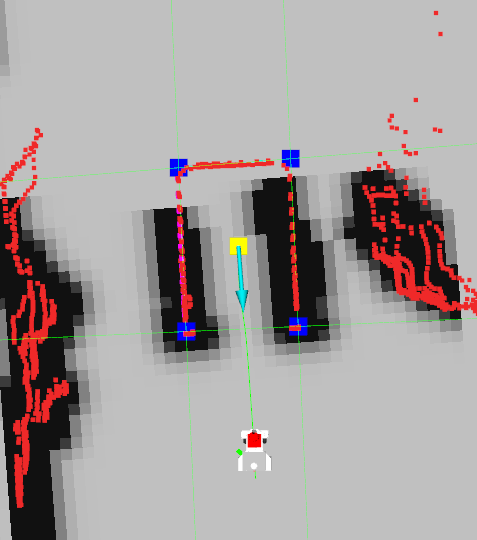
\includegraphics[width=0.3\textwidth]{pics/detection_success.png}
    \caption{\textsc{Successfully Detected Container Shape}}
    \label{fig:detection_success}
\end{figure}
As a result of a successful execution of \code{DETECT_CONTAINER}, either two or four corners are detected and passed to the next state. If only two corners, i.e. the entry, are
detected, \code{ALIGN_ROBOT_TO_RAMP} follows. If, on the other hand, four corners are detected (cf. fig. \ref{fig:detection_success}), this state is skipped and \code{DRIVE_INTO_CONTAINER} follows, since the entire
container has already been detected. In \code{ALIGN_ROBOT_TO_RAMP}, the robot is aligned in front of the container based on the detected entry. The target pose is passed as the
output of \code{DETECT_CONTAINER} and the robot navigates there. Subsequently, \code{DRIVE_INTO_CONTAINER} follows. If the transition came from \code{DETECT_CONTAINER}, i.e. if
\code{ALIGN_ROBOT_TO_RAMP} was skipped, all four corners were already detected in the previous state, which are now utilized. If, on the other hand, it follows the state
\code{ALIGN_ROBOT_TO_RAMP}, there is no input and the robot should detect the entire container from this improved position. In both cases, based on the four detected corners,
a pose is computed in the center, facing the entrance, and the robot is navigated there (cf. cyan arrow in fig. \ref{fig:detection_success}). Thereafter, \code{LOCALIZE_CHARGING_STATION} starts using the input corners detected in the
previous state as input. As the mounting position of the charging station within the container is known, the target position for the alignment in front of it can be calculated
relative to the detected container shape. Afterwards, the robot is moved there in \code{ALIGN_ROBOT_TO_CHARGING_STATION} and the whole execution of the state machine ends in
\code{DOCK}. Analogously, the undocking state machine ensures that the robot leaves the container after a successful charging procedure and can continue its mission.\newline
This (un-)docking solution can be used for both planned charge stops as well as unexpected but necessary stops detected by monitoring processes such as the one described in section
\ref{sec:battery_monitoring}. Concluding, it is easy to configure whether the simulation should use the docking solution in combination with the container model or only the simplified
charging patch. Similar to Hawes et al. \cite{Hawes:2017} and Pinillos et al. \cite{Pinillos:2016}, one could exploit the fact that the
robot keeps returning to the charging station by resetting the position to the location inside the container aligned in front of the charging station to avoid cumulative localization
errors. In contrast to the scenario considered there, however, the exact position of the container is not necessarily assumed to be known, but it must be detected within a certain
range. Nevertheless, it will certainly be the same within a mission, so one can expect to use it as a landmark after the initial detection.\newline

\chapter{Experiments and Evaluation}
\label{sec:experiments}

The general idea behind the upcoming experiments is the following simple scheme: problem simulation by publishing on the respective topic, followed by a triggered monitoring
procedure that should detect the problem, interrupt normal operation, and initiate an appropriate resolution. Either it succeeds and \code{NORMAL_OPERATION} continues, or it cannot be
resolved and execution ends in \code{CATASTROPHE}.\newline
Hawes et al. introduce two useful metrics to evaluate the performance of a long-term autonomous system: the total system lifetime and the autonomy percentage. \cite{Hawes:2017} The
first measures the time the robot was in autonomous operation and is reset when an unrecoverable failure or an unrequested intervention of the human operator is required. However,
it does not make sense to evaluate this time when it certainly depends on the frequency with which the failures that are considered in this work are simulated. The second metric
(autonomy percentage), on the other hand, is very useful for this work as well. \textquote{\textit{The motivation of the autonomy percentage is that it is of little value to achieve a long
total system lifetime if the system does nothing}}. \cite{Hawes:2017}
Steinberg et al. \cite{Steinberg:2016} introduce the metric of time between undesired human interventions. By undesired situations, they mean situations in which the robot should
in principle be able to recover itself, as opposed to situations in which human intervention is expected. Applied to this work, this could refer to LTA failures for which specific
solutions or workarounds have been proposed but do not succeed (cf. \ref{sec:solutions_for_lta_challenges}). Furthermore, they propose a metric for information sharing, i.e. the
percentage of time the robot communicates meaningful information to the operator.\newline

TODO: Hardware + real-time factor information\newline

\textit{Demonstration of the Basic Functionality of the Integrated System.}\newline

The very first step is to show that without simulating any of the identified LTA problems, the mission runs flawlessly for an extended period of time, e.g., $5$ hours. This serves as
a verification of the sample plan, i.e. it shows that the charging stops are sufficient if everything works as expected. Furthermore, it is a demonstration of the fundamental
functionality of the entire integrated system in the absence of unexpected problematic events. For evaluation purposes, let a failed mission be defined as a mission that exceeds a
user-configurable timeout $t = 900s$ without publishing a message to \code{arox/ongoing_operation}, although the previous message contained a value of \code{total_tasks} that is
greater than one, indicating that the current plan is not completed and thus that the robot has been stuck in that task for a time greater than $t$. Obviously, a \code{severe_failure}
in the low-level state machine leading to a \code{CATASTROPHE} state followed by a system shutdown is also considered a failed mission. This would be the result of a completely
discharged battery. To endow this test of basic functionality with some significance, it was performed three times. Most importantly, all runs were completed without failure. Thus,
unsurprisingly, the average runtime was $5.09$ hours. In this time, the robot has completed an average of $3.67$ missions and $106.67$ tasks. The robot required an average of $9.67$
charge cycles and the average total distance traveled was $1102.68 m$. It is also interesting to look at the mode distribution, i.e. how long the robot was in which mode during the LTA
episodes, which is shown in Fig. \ref{fig:mode_times_basic}. [TODO: Explain real mode dist]
\begin{figure}[H]
    \centering
    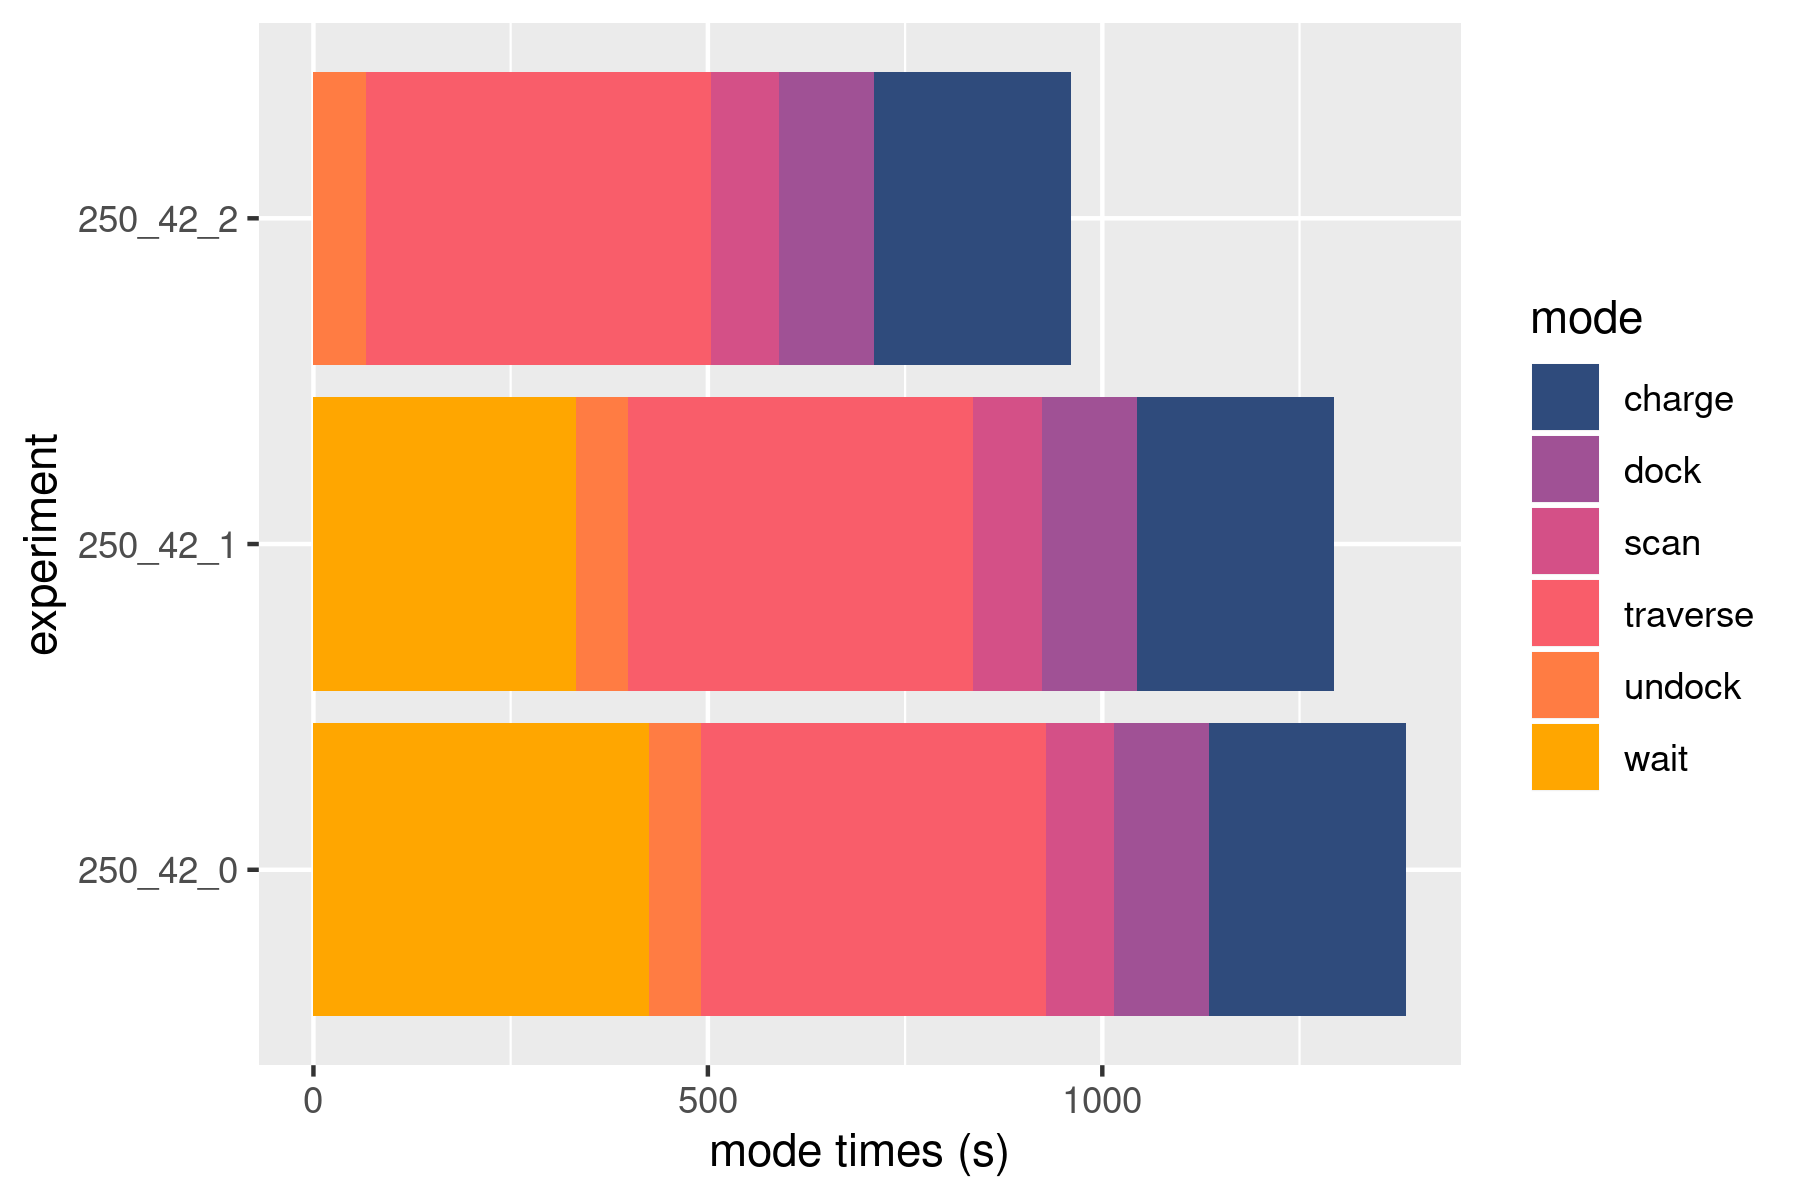
\includegraphics[width=0.75\textwidth]{pics/mode_times_basic.png}
    \caption{\textsc{Mode Distribution}}
    \label{fig:mode_times_basic}
\end{figure}
The slight discrepancy in the number of successfully completed tasks between runs results from the fact that, for instance, the docking procedure does not always detect the container
at the same speed. In general, the simulation has certain non-deterministic aspects in the sense that the combination of all the ROS nodes, their communication, possible effects in
the simulation, and execution times mean that two runs of such an experiment in simulation will certainly not be exact reproductions of the same states. Although the three runs do not
guarantee a fundamentally error-free use of the system, they demonstrate that the basic expected stable functionality is given.
The detailed results can be found in the appendix (cf. fig. \ref{fig:detailed_functionality_res}).\newline

\textit{Classification of the Selected LTA Problems.}\newline

The classification of the selected LTA problems is based on their evaluation in the simulation together with a comparative contextualization of the practical case. The aim is to
classify the identified problem categories in the simulation according to their severity, i.e., which LTA problem can lead to which worst-case outcome. By definition, all identified
problems can lead to contingencies, as outlined in the corresponding sections (cf. section \ref{sec:sim_and_mon_of_lta_challenges}). Additionally, all of them can lead to
catastrophes, at least as a fallback option in case of resolution failures. However, this implies monitoring to detect the problems. As a brief recap, contingencies are situations in
which the robot's ability to act is essentially preserved, so that it can attempt to solve the problem itself. Catastrophes, on the other hand, definitely require human intervention.
Hence, when the proposed monitoring framework is active, each problem category can potentially lead to the worst case outcome of \code{CATASTROPHE}. More interesting in terms of
classification is the present state of the AROX system, i.e. no monitoring for the identified issues. In this case, \code{CATASTROPHE} refers to one of the two aforementioned
conditions - battery failure or timeout - and is thus equivalent to mission abort. The first category is LTA problems that, when they occur, prevent the successful continuation of the
mission in the simulation. Despite the fact that it is evident for some of the identified problems for LTA operations (e.g. power management failures) that they are capable of
interrupting the mission, it is systematically investigated how the system in simulation responds to these failure cases without the developed monitoring procedures. This is critical to verify the
correct and expected behavior of the simulated fault cases. Power management failures are the first case to be considered. When simulating a power management failure, e.g. by
publishing on \code{/sim_power_management_catastrophe}, the battery discharge rate is increased without the robot noticing, so it simply runs out of battery and normal operation
ends with a \code{severe_failure}, leading to a transition to \code{CATASTROPHE} and then a system shutdown. Thus, the simulation of power management failure works as expected. That
the general error class of charging failures can lead to a failed mission can be demonstrated by simulating a docking error that results in not being able to recharge and also
ends in \code{CATASTROPHE}. Hence, without active monitoring, \code{/sim_docking_failure_raised_ramp} is used to verify this. As expected, this also ends with a completely
discharged battery and thus a failure of the mission. Evidently, both cases lead to a failed deployment in practice with the real robot as well, which would go unnoticed without
monitoring. The first example that cannot interfere with the operation in the simulation is drastic weather changes. Since these phenomena are not explicitly simulated in
\textit{Gazebo}, but are only indicated by corresponding messages on the weather monitoring channels, without active monitoring for these messages, the robot simply does not recognize
this. The same is true in practice: the robot would continue its mission without detecting a change in circumstances. Therefore, the mission would continue as long as possible, that
is, as long as the robot is not damaged. This is of course highly risky and can result in the robot being damaged or the sensor data being worthless. Consequently, it is apparent that
the monitoring of these phenomena is necessary. However, drastic weather changes per se will never lead to a \code{CATASTROPHE}. Naturally, if the robot gets damaged, catastrophic
situations could occur, indirectly caused by drastic weather changes. Analogously, without the active monitoring, errors in sensor perception and data management would simply be
disregarded and go unnoticed. The robot's operation is not affected, but the results are of course worthless or not even saved, both in practice and in simulation. The
connection-related failures can be considered separately. WiFi outages do not affect the mission in the simulation, and in practice it depends on the exact use of the connection in
the considered scenario. If the RTK correction signal is sent via WiFi, localization may be compromised.  Additionally, if the scans are transferred via WiFi, the results may be lost
and the entire mission may become a futility. The same applies to an internet connection, where several parts of the system can be affected. Finally, GNSS-related failures can
directly lead to navigation failure even in simulation. For instance, \code{/toggle_simulated_teleport}, which manipulates the latitude or longitude estimates, can drastically
falsify the robot's localization and cause arbitrarily severe failures. The robot could travel in dangerous or unsuitable places, or it could simply find itself in a situation that it
cannot leave and, in the best case, completely discharges its battery, leading to a \code{CATASTROPHE} or to the fact that it can no longer perform any tasks, so that the mission fails
due to the timeout criterion introduced above. Moreover, plan distribution errors or navigation failures such as obstacles surrounding the robot, e.g. the \textquote{robot prison}
case in section \ref{sec:sim_and_mon_navigation_failures}, are simply not detected, but the mission can fail due to the timeout criterion or a completely discharged battery
(\code{CATASTROPHE}), whichever comes first. Failure is guaranteed for plan distribution errors and possible for navigation errors. This again holds for simulation as well as for
practice. That localization errors can have dramatic consequences up to \code{CATASTROPHE}
cases has already been shown by the example of GNSS connection issues. The findings of the classification are summarized in fig. \ref{fig:lta_classification}. Crucially, any problem
category that has a \textquote{\cmark} or \textquote{(\cmark)} in the catastrophe column has the potential to abort the mission without monitoring solutions. Assuming persistent
failures, \textquote{\cmark} means that mission abort is a certainty, while \textquote{(\cmark)} stands for the possibility. Another perspective is that \textquote{\cmark} refers to
catastrophes caused directly by the problem, the problem itself causes the failure, not some effect on another aspect of the system, whereas \textquote{(\cmark)} stands for indirect
causation. Furthermore, the remaining problems of drastic weather changes, sensor failures, and data management issues do not interrupt the mission, but they do invalidate the results
and thus have the potential to render the mission worthless both in practice and in simulation. There is only one exception: drastic weather changes in the simulation. As already
anticipated, the actual occurrence of such events is not simulated, only the information of their presence. However, since the practical relevance is obvious, there is no need for
further simulation of e.g. impaired scans due to bad weather conditions. In summary, all of the identified issues have the potential to render LTA deployments worthless in real-world
scenarios, clearly highlighting the importance of addressing all of these problems if one aims to operate robots long-term autonomously in an outdoor context.
\begin{figure}[H]
    \centering
    \resizebox{\textwidth}{!}{
    \begin{tabular}{| c | c | c | c | c |}
        \hline
        \textbf{problem} & \specialcell{\textbf{contingency \& catastrophe} \\ \small{\textit{(with monitoring)}} \\ sim / prac} & \specialcell{\textbf{catastrophe} \\ \small{\textit{(without monitoring)}} \\ sim \quad\quad\quad\quad prac} & \specialcell{\textbf{potential to render mission worthless} \\ sim \quad\quad\quad\quad prac} \\ \hline
        power\_management & \cmark & \cmark \quad\quad\quad\quad\quad \cmark & \cmark \quad\quad\quad\quad\quad \cmark \\ \hline
        charging\_failure & \cmark & \cmark \quad\quad\quad\quad\quad \cmark & \cmark \quad\quad\quad\quad\quad \cmark \\ \hline
        drastic\_weather\_change & \cmark & \thinspace\thinspace \xmark \quad\quad\quad\quad\quad (\cmark) & \xmark \quad\quad\quad\quad\quad \cmark \\ \hline
        sensor\_failure & \cmark & \xmark \thinspace\thinspace\quad\quad\quad\quad\quad \xmark & \cmark \quad\quad\quad\quad\quad \cmark \\ \hline
        data\_management & \cmark & \xmark \thinspace\thinspace\quad\quad\quad\quad\quad \xmark & \cmark \quad\quad\quad\quad\quad \cmark \\ \hline
        lost\_connection & \cmark & (\cmark) \quad\quad\quad\quad (\cmark) & \cmark \quad\quad\quad\quad\quad \cmark \\ \hline
        plan\_deployment\_failure & \cmark & \cmark \quad\quad\quad\quad\quad \cmark & \cmark \quad\quad\quad\quad\quad \cmark \\ \hline
        navigation\_failure & \cmark & (\cmark) \quad\quad\quad\quad (\cmark) & \cmark \quad\quad\quad\quad\quad \cmark \\ \hline
        incorrect\_localization & \cmark & (\cmark) \quad\quad\quad\quad (\cmark) & \cmark \quad\quad\quad\quad\quad \cmark \\ \hline
    \end{tabular}}
\caption{\textsc{Classification of LTA Problems in Terms of Severity}}
\label{fig:lta_classification}
\end{figure}

\vfill
\pagebreak

\textit{Evaluation of the Monitoring Framework.}\newline

In general, the experimental evaluation is based on the process that has already been followed throughout the work: Problem simulation, monitoring and subsequent solution. The
simulations of error cases, as they can be taken from section \ref{sec:sim_and_mon_of_lta_challenges}, can always be activated by a message on the corresponding topic. Then, a
monitoring node should detect the problem, interrupt \code{NORMAL_OPERATION}, and initiate an appropriate resolution. The resolver either solves the problem and then returns to
\code{NORMAL_OPERATION}, or it cannot solve the problem and proceeds to \code{CATASTROPHE}. In the previous section, it was shown that all of the problems identified indeed have the
potential to render the mission worthless. Moreover, none of them can be detected by the AROX system without the developed monitoring framework. Now the natural question is to what
extent the developed monitoring framework improves the situation. This section is about assessing the reliability of the monitoring solutions, i.e. the degree to which the monitoring
nodes are able to detect and solve / communicate the problems when they occur. To this end, a series of experiments were conducted. The idea is to run an LTA episode and randomly
simulate the occurrence of issues from the set of identified problem categories at a user-configurable frequency by publishing to the respective topic. Since it is always known which
reaction is expected after a certain simulation, the expected can be compared with the observed. It is essentially based on a dictionary that maps the fault simulation topics to the
corresponding expected error messages on the \code{contingency_preemption} topic. The following results are based
on a frequency of $250s$, i.e., a random problematic situation occurs every $250s$. However, the $250s$ are only a lower bound on the time between two fault simulations because some
of the simulations can only occur in certain situations, such as when the robot is stationary, so they are only run when that situation occurs next, and there are never two
simultaneous fault simulations. Furthermore, the $250s$ are real time and since the RTF in \textit{Gazebo} was only about $0.2$, the average frequency in the simulation should be
$\approx 1250s$. The frequency was not chosen too high, so that the robot can still perform tasks and is not only occupied with error handling.
In order for the evaluation to be reasonably meaningful, the experiments must be of a certain length. At the same time, they must be feasible within the restrictive
time constraints of this thesis. As a compromise, the time per run was set at $5$ hours. Experimentally, it turned out that this runtime is sufficient to achieve a certain validity,
since several mission and charge cycles occur and there is enough room for error simulation. This $5$-hour episode was repeated $10$ times. The intention behind the repeated
experiments is on the one hand to endow the conclusions with some significance, but on the other hand also to be able to judge how many of these runs ended in a \code{CATASTROPHE} and
how many ran successfully to the end. Ideally, there should be no missions that end in a \code{CATASTROPHE}, since only problems that are in principle solvable are simulated for this
experiment. However, if a resolution fails, for example, a \code{CATASTROPHE} case can still occur, leading to the end of the episode. In order for the runs to be comparable, the
random selection of failure simulation was initialized with the same seed leading to the same sequence of simulated problems. In the future, further experiments should be conducted
with different seeds to cover the full range of simulated failures. Both plots presented in fig. \ref{fig:evaluation_res} show the experimental runs on the $y$ axis using the following
naming scheme: \code{frequency_seed_idx}. The frequency refers to the failure frequency in seconds, i.e. how often a random failure is triggered, the seed is used to initialize the
random number generator for selecting the simulated error, and the index simply identifies the individual runs.
As can be observed, $8/10$ runs completed successfully without a \code{CATASTROPHE} case. The two aborted runs are the result of docking failures that could not be resolved.
This still happens from time to time at the moment, but is not a flaw of the monitoring framework, but rather a matter of robustness of the integrated docking solution presented
in section \ref{sec:docking_solution}. Thus, the problems did occur and were correctly identified and communicated by the monitoring framework.
Fig. \ref{fig:expected_res} shows the expected response to error cases per run in percent.
Ideally, this would be $100\%$, which would mean that the monitoring detects exactly all simulated problems and nothing beyond, which was the case in several runs ($0, 3, 5, 6, 7$).
This proportion is composed of correct \code{CONTINGENCY} cases, i.e. when exactly the expected case occurs, which means that the monitoring worked correctly, and correct
$\lnot$\code{CONTINGENCY} cases, where there is no \code{CONTINGENCY} expected and none occurs. Correct $\lnot$\code{CONTINGENCY} situations refer to cases where the simulated problem
is so minor that it should be handled by the robot without initiating a contingency or catastrophe. A good example of such a case are the simulated static obstacles with an escape
route displayed in fig. \ref{fig:obstacle_scenarios}. In this particular case, the purpose is to test that navigation error monitoring is not configured too aggressively and does not
trigger \code{CONTINGENCY} in the event of a sustained recovery with progress. Figure \ref{fig:obstacle_success} shows how the robot successfully deals with the obstacles by
iteratively approaching the goal. In such a situation, there should be no interruption of the normal operation. In general, across the problem categories, there are some cases that
are somewhat problematic but do not cross the boundary of \code{CONTINGENCY}, i.e., do not require interruption of the normal operation. Thus, the $\lnot$\code{CONTINGENCY} category
is used to verify that the monitoring solutions are not configured too restrictively to ensure that the robot does not constantly try to solve imaginary problems. The remaining
unexpected responses are composed of false-positives, i.e. \code{CONTINGENCY} cases with no simulated failure, false-negatives, i.e., cases where a failure simulation would require
a \code{CONTINGENCY} but the problem is not detected by the monitoring nodes, and finally unexpected contingencies, which refer to cases where a \code{CONTINGENCY} is expected due to
a simulated failure but a different type of problem is detected. It is very crucial to note that false positives and unexpected contingencies are not necessarily a
fault of the monitoring framework or its configuration. A significant majority of the cases is related to problems in the simulation that were not simulated as part of an experiment,
but actually occur and are thus correctly detected by the monitoring framework. For instance, docking errors occur from time to time simply due to the robustness of the integrated
docking solution. Once the monitoring framework detects such a non-simulated problem, it is considered a false positive or unexpected contingency, depending on the circumstances,
even though it is perfectly correct to identify the problem. In order to actually evaluate the performance of the monitoring framework and not include other aspects such as the
robustness of the docking solution, these correctly identified but not simulated problems are manually removed from the results to allow reasonable conclusions to be drawn at the
end. Ideally, the results post-processed in this way will contain no or few false positives and false negatives, indicating that the monitoring detects exactly what is actually
problematic and no more. 
On average, the number of simulated problem cases is $13.75$ per episode. The average proportion of expected responses to these error cases across all runs is
$95.89\%$, which highlights a fairly reasonable reliability of the system. The few unexpected responses consist of some false positives with respect to localization problems.
Apparently, some of the monitoring approaches are configured to be too sensitive. In addition, there were a total of two false negatives for the same simulated problem, namely
divergence between odometry and GNSS estimates of the total distance traveled. This is most likely due to the fact that the way this is simulated is not perfect for all circumstances
and should be fairly easy to resolve in the future. Moreover, on average, the robot completed $3$ missions with a total of $88.75$ tasks and required an average of
$10.38$ charge cycles. Per episode, the robot traveled an average total distance of $967.1$ meters in $5.06$ hours, estimated from odometry data. Another interesting aspect of LTA systems
discussed in the literature is the autonomy percentage, i.e. the time during which the robot actually performs autonomous tasks, excluding idle time, etc. The autonomy percentage for
the performed experiments is depicted in fig. \ref{fig:autonomy_percentage} and illustrates that the majority of the runtime is spent on actual autonomous tasks, on average $96.28\%$.
\begin{figure}[H]
    \centering
    \begin{subfigure}[b]{0.49\textwidth}
        \centering
        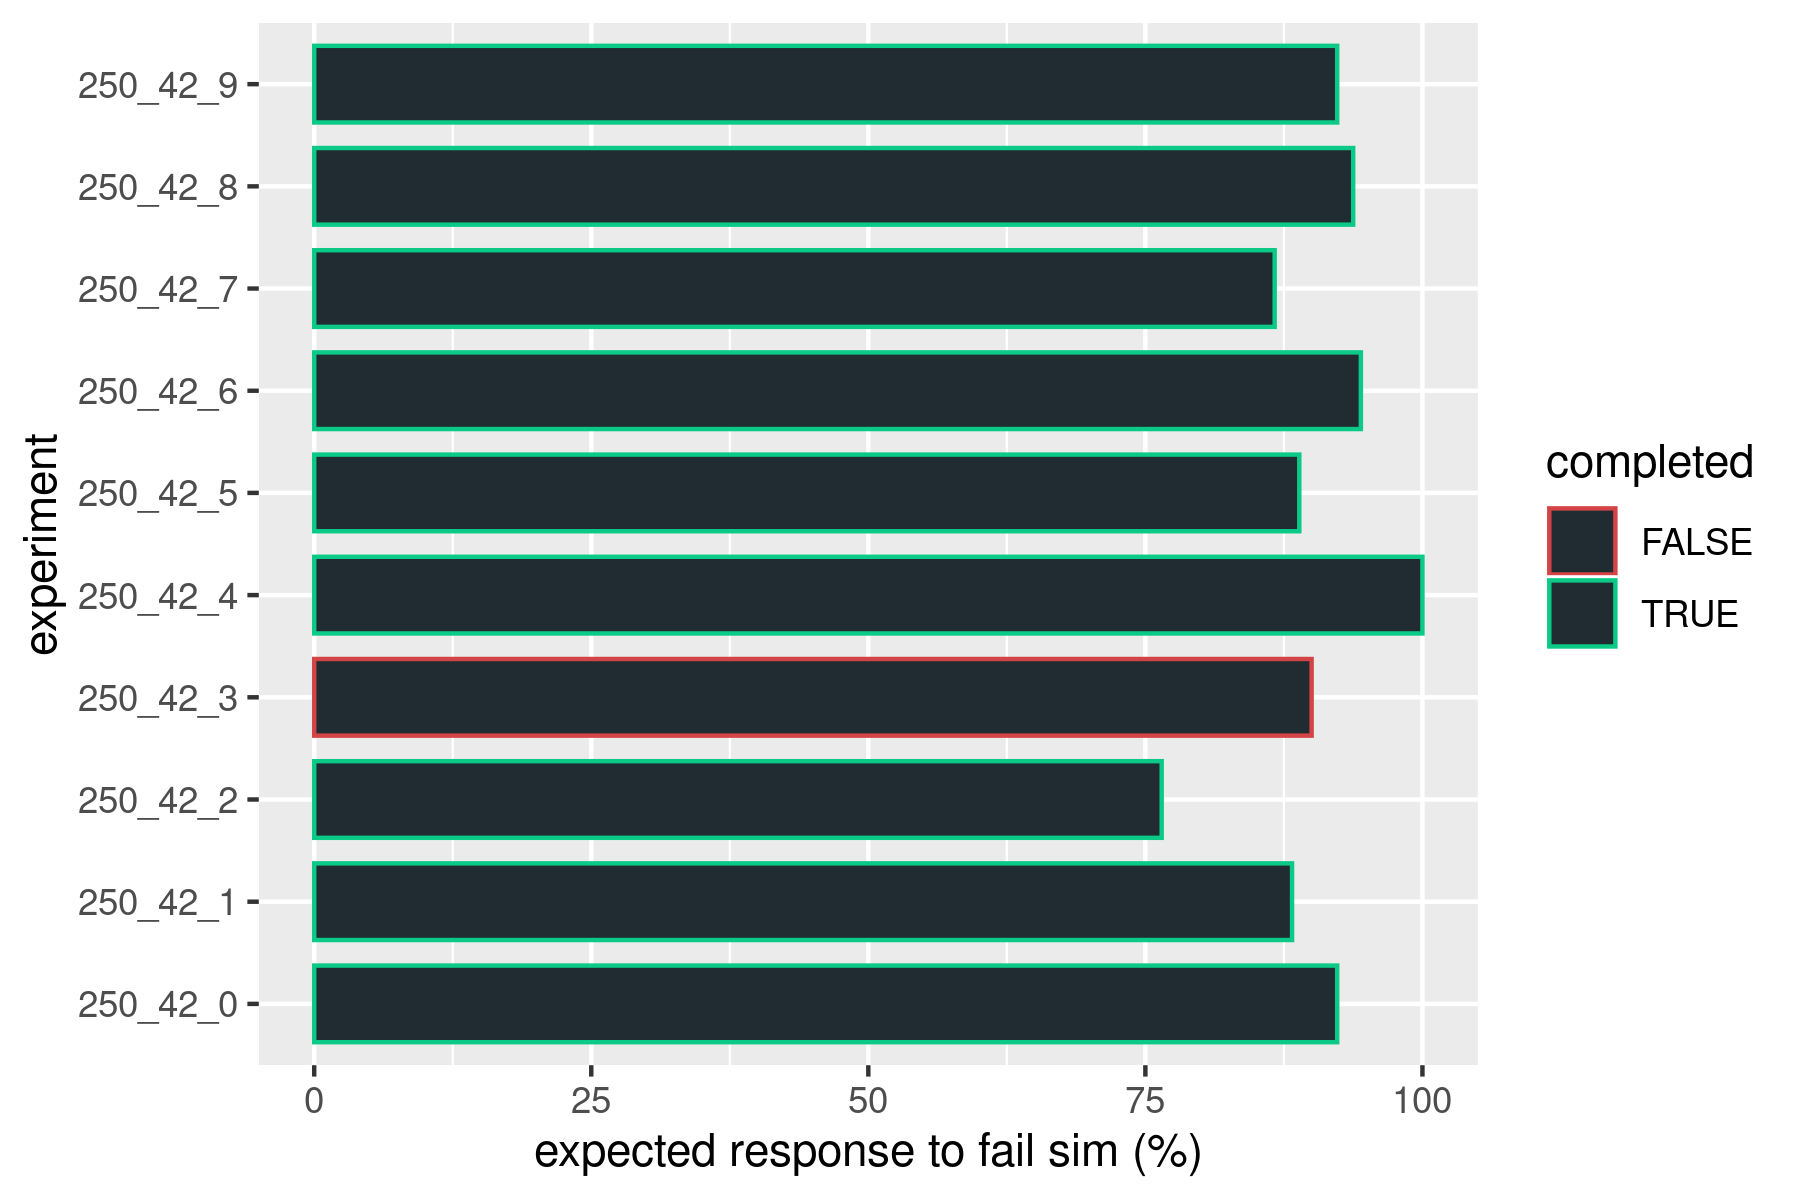
\includegraphics[width=\textwidth]{pics/expected_res.png}
        \caption{\textsc{Expected Response}}
        \label{fig:expected_res}
    \end{subfigure}
    \hfill
    \begin{subfigure}[b]{0.49\textwidth}
        \centering
        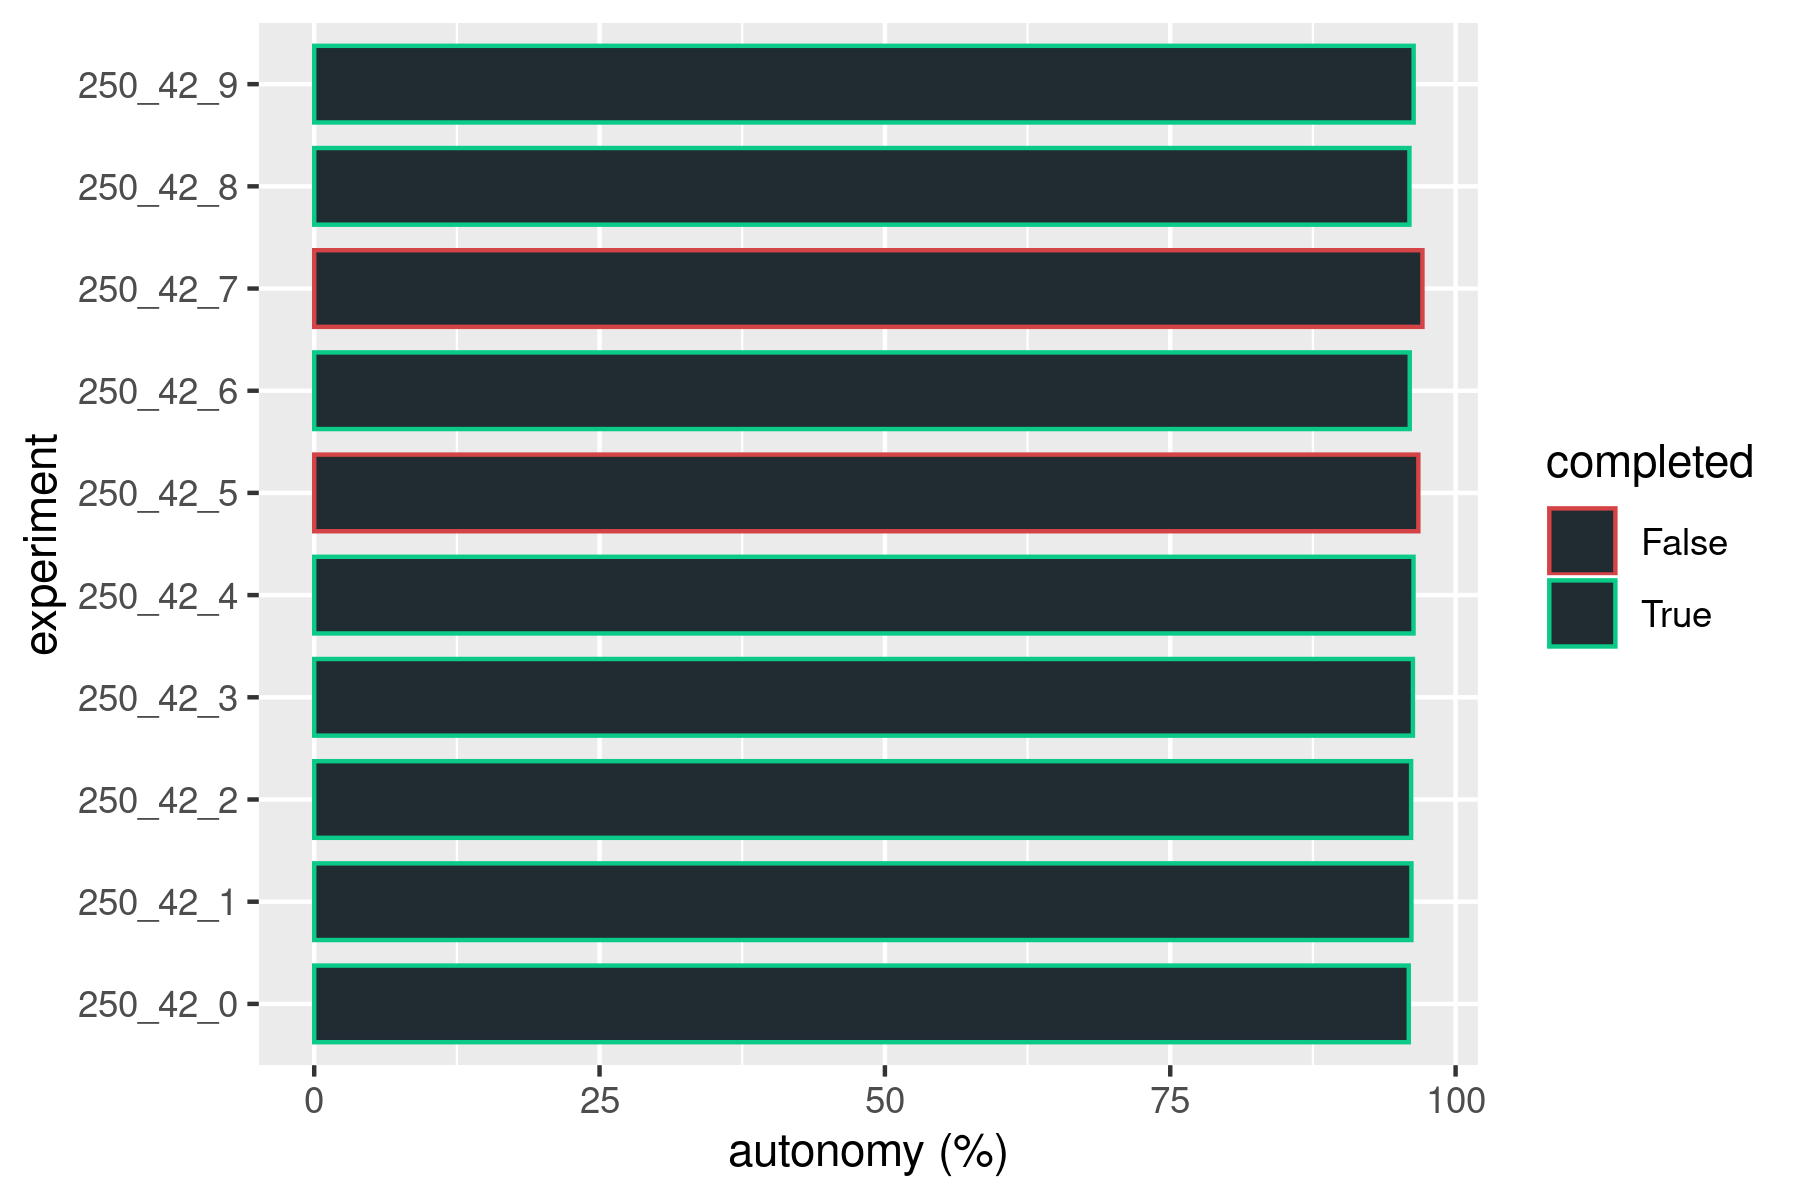
\includegraphics[width=\textwidth]{pics/autonomy_percentage.png}
        \caption{\textsc{Autonomy Percentage}}
        \label{fig:autonomy_percentage}
    \end{subfigure}
\caption{\textsc{Evaluation Results}}
\label{fig:evaluation_res}
\end{figure}
Also revealing is the activity distribution, i.e. how much of the runtime the robot spends on which activity or in which mode.
This contextualizes the autonomy percentage quite well, and again it can be seen that the robot spends little time waiting and most of its time driving and scanning.
Beyond that, (un)docking and charging naturally takes some time as well.
\begin{figure}[H]
    \centering
    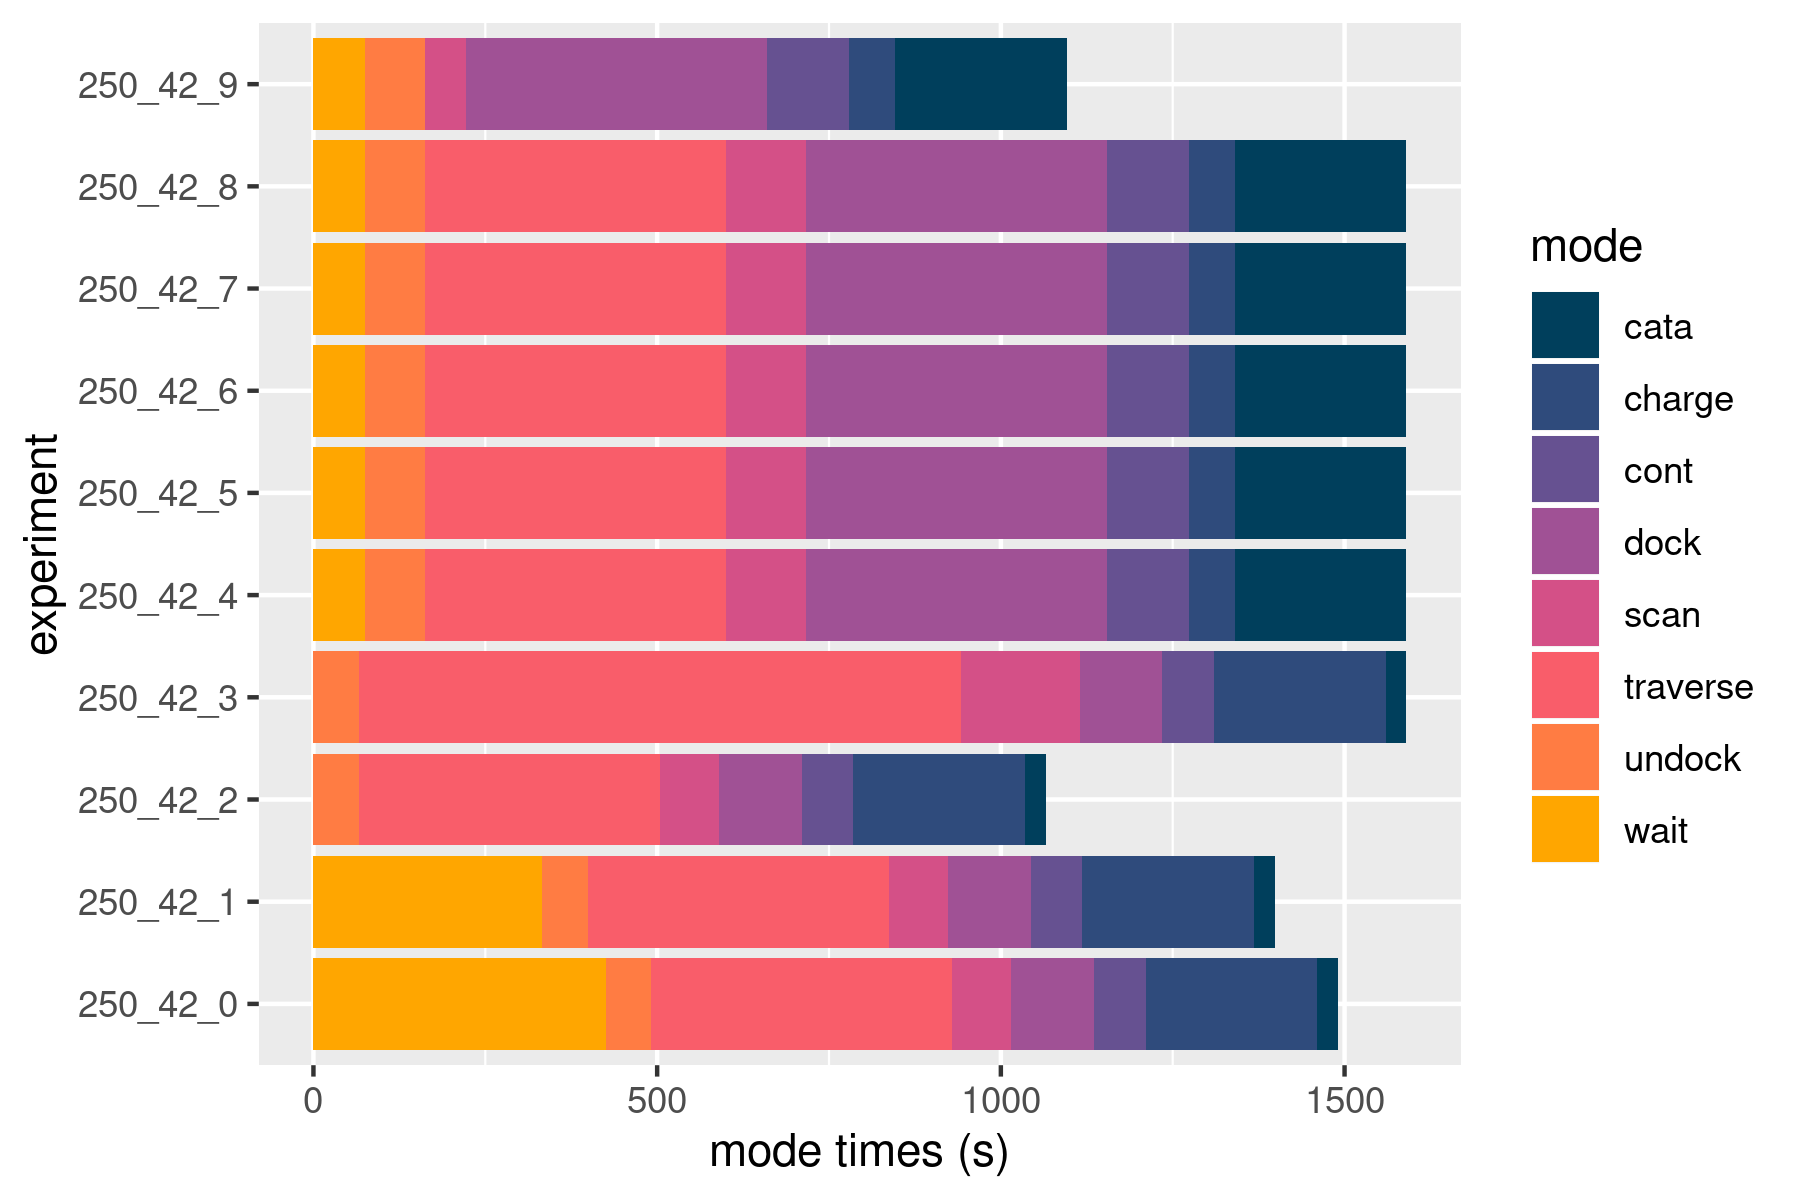
\includegraphics[width=0.75\textwidth]{pics/mode_times.png}
    \caption{\textsc{Mode Distribution}}
    \label{fig:mode_times}
\end{figure}
Based on the results, in can be concluded that the proposed framework drastically improves the resilience with respect to the identified challenges. The initial goal of assigning each
of the identified problem categories to a different category was achieved, and the experiments demonstrate a certain level of reliability in doing so. The detailed results can be
found in the appendix (cf. fig. \ref{fig:detailed_monitoring_eval_res}).

\vfill
\pagebreak

\chapter{Conclusion and Future Work}
\label{sec:conclusion_future_work}

\section{Conclusion and Discussion}

Since this work is at least partly integrative in nature, the first important aspect is that the functionality of the overall integrated system has been demonstrated.
Practically relevant challenges to the long-term autonomy of mobile outdoor robots were identified, classified in terms of their potential impact, and implemented in simulation.
As anticipated in section \ref{sec:challenges_for_lta}, the goal of the work with respect to the identified problems was to shift the selected subset of problems into category
$(1)$ or $(2)$ based on the classification in fig. \ref{fig:problem_types}, i.e. to enable the robot to solve or at least recognize them in order to communicate them.
Since monitoring approaches have been proposed for each of these categories (cf. section \ref{sec:sim_and_mon_of_lta_challenges}), this goal can be considered achieved. These
monitoring approaches are incorporated into a generic monitoring and resolution framework developed as part of this thesis, with an emphasis on a certain degree of universality.
This is manifested in the fact that as few assumptions about specific systems and scenarios were made as possible. One requirement, though, was that the system is conclusively usable
in practice in the considered context, which presupposes that not only abstract high-level architectures are defined, but that a compromise is found between the greatest possible
universality and simultaneous applicability in the scenario under consideration. This results in the fact that the universality ends when leaving the ROS cosmos, i.e. the system is
exclusively designed for ROS systems. While certain lines of reasoning and observations in this thesis may apply to non-ROS systems as well, there is at least no practical
applicability of the developed framework to these systems. Due to the high prevalence of ROS coupled with the requirement to be practically applicable, the restriction to
compatibility with ROS systems seems reasonable.
The reliability of the framework has been experimentally endorsed, at least in simulation. In total, there are $48$ problem instances that can be explicitly triggered
through simulation by publishing on a topic, as presented in section \ref{sec:sim_and_mon_of_lta_challenges}. Beyond that, there are many other problem cases that are explicitly
covered by the monitoring procedures. However, there are also numerous potential problem cases that are not explicitly considered by the monitoring nodes, but are nevertheless
implicitly covered and thus detected. For instance, a situation in which the robot falls over is neither explicitly recognized nor communicated. Yet at the latest when the expected
battery consumption no longer matches the actual situation, i.e. the robot has to recharge, a problem is detected and communicated. This also illustrates the fact that the problems
identified are not strictly separated, but that the transitions are somewhat fluid. Since the considered system was previously not able to deal with the identified problems at all
and each of these problems has the potential to make the mission fail, it is evident that the proposed approaches significantly improve the robustness of the system with respect to
the identified challenges. Since the purpose of this work was not only to identify and deal with the problem categories, but also to define an architecture that allows systematic
handling of such situations, it should be noted that the overall architecture has proven to be suitable for this type of non-nominal plan execution. In particular, due to the parallel
running monitoring nodes, the tight coupling of \textit{acting} and \textit{monitoring} in general, and the modularity that enables extensibility and reconfigurability.
In conclusion, all identified problems are detected with indications of quite high reliability and some of them can even be solved by the robot itself.
It is crucial to mention that even if an episode fails, as in the two cases of experimental evaluation in section \ref{sec:experiments}, catastrophe cases are always communicated to
the human operator, which is a huge improvement over the situation without the developed framework, where a total failure would go unnoticed.\newline

\noindent
As outlined in the introduction of monitoring techniques in section \ref{sec:sim_and_mon_of_lta_challenges}, monitoring is in principle applicable to other ROS systems if the
introduced slight constraints in terms of information provision based on the defined ROS messages and topics are met.
However, the tight coupling between the deliberation functions of \textit{acting} and \textit{monitoring}, which is not a mere by-product but is intended in this work, results
in the framework not being usable \textquote{out-of-the-box} for other systems. It should not be considered a weaknesses, though, as this coupling is necessary for the two functions to be
mutually beneficial, so \textit{acting} provides context to \textit{monitoring} and \textit{monitoring} is able to directly intervene in \textit{acting} when necessary. Furthermore,
it should be relatively simple to establish this coupling with the operational models of other systems as well. In order to be able to achieve this without too much effort and also
quite intuitively, the architecture proposed in this work was built in a modular way. Thus, in order for another robotic system to use the monitoring framework without using the
operational model used in this thesis, the embedded \code{OPERATION} state machine shown in fig. \ref{fig:high_level_smach} would have to be replaced by the system's own operational
state machine, which is either also implemented as \code{SMACH} or at least wrapped by one. There are some assumptions that such an operational state machine must satisfy. First, it
must communicate information about the mode of the system via \code{arox/ongoing_operation} in the form of \code{arox_operational_param.msg}. Once again, the naming scheme is somewhat
misleading in terms of universality, but is retained for the moment for the sake of compatibility with the integrated battery watchdog module. The available modes are \code{scanning},
\code{traversing}, \code{waiting}, \code{docking}, \code{undocking}, \code{charging}, \code{dead}, \code{contingency} and \code{catastrophe}. Most of them should be useful in any
context where the monitoring framework is to be used. However, not all of them need to be adopted. Another crucial aspect is that all active goals should be interruptible via a
message on \code{/interrupt_active_goals}, e.g. by using \code{actionlib.SimpleActionClient} and \code{cancel_all_goals()} for the tasks. To utilize resolution attempts during
navigation failures, extreme weather conditions, and power management failures, the topics \code{/introduce_intermediate_nav_goal}, \code{introduce_intermediate_recharge_goal},
\code{introduce_intermediate_shelter_goal}, and \code{stop_waiting} should be provided. Most of them are self-explanatory, \code{stop_waiting} is used to stop waiting in the
shelter, e.g. after extreme weather situations. Eventually, the outcomes must be compatible with the architecture shown in fig. \ref{fig:high_level_smach}, i.e.
\code{minor_complication}, \code{critical_complication}, \code{end_of_episode}, and \code{preempted}. A further important note with regard to the general applicability of the
framework is that each monitoring node can easily be removed, i.e. deactivated. Presently, this can be achieved by simply removing the option from the framework's launch file.
For instance, if a mobile outdoor robot is used without a Lidar scanner, the sensor monitoring node can simply be removed. Analogously, custom monitoring nodes can be added to the
framework by simply adding the nodes to the launch file and supporting the described architecture by publishing to \code{contingency_preemption}, etc. Thus, the idea is that
context-dependent special solutions can be easily added, removed and replaced by other specific solutions.

\section{Future Work}

Now that the presented framework performs well in simulation, a natural next step is to conduct field tests and demonstrate it on the real AROX platform. Furthermore, the meaningful
use of the presented \code{data_accumulator} is only possible with actual data from real long-term autonomy experiments. As announced, the idea is to learn from experience, which
obviously requires data from real-world experiments. While the logging aspect and basic functionality has already been part of this work, actually collecting real-world data from
long-term autonomous missions and then learning from that data is a step for the future. Beyond that, however, further experiments in simulation can be revealing. For instance, the
$10$ runs in the evaluation section were always initialized with the same seed, thus also always with the same sequence of problems simulated to have some comparability between runs.
Of course, there should be more experiments in the future that cover the entire set. In addition, variations in runtime and error frequency should be investigated. Since the focus of
this thesis was on monitoring and only simple workarounds were implemented, there is obviously great potential for future work in developing more elaborate solution techniques.
However, even simple contextual recovery behaviors could be easily defined and integrated and be of great use in practice.
Another practically useful aspect for future improvements would be a web interface that would allow remote access to sensors as well as direct control of the robot. This way, an
operator could take control for a short time in case of minor problems and would not have to be physically on site. Yet a simple improvement in communication with the operator would
also be of great benefit. So far it has been implemented in pure text form, but it is easy to imagine an improved version with graphically processed sensor, weather and other
information via a web interface. Ultimately, a truly crucial aspect is usability, i.e., the integration and reconfiguration of the developed framework. Throughout the work, it was
pointed out that great emphasis was placed on a certain universality and generic solutions. Although most of the implemented approaches are generally applicable to many scenarios due
to this focus, there is still much room for improving and simplifying the integration and reconfiguration of the monitoring framework.

\bibliography{papers}

\begin{appendices}
    \chapter{Detailed Results of Questionnaire}
    \label{sec:detailed_questionnaire_results}

    \begin{figure}[H]
        \centering
        \resizebox{0.75\textwidth}{!}{
        \begin{tabular}{| c | c | c | c | c |}
            \hline
            \textbf{problem} & \textbf{impact} & \textbf{difficulty} & \textbf{likelihood} \\ \hline
            charging\_failure & [1, 2, 1, 1, 2, 1, 1] & [1, 2, 1, 2, 1, 1, 1] & [2, 2, 2, 1, 3, 1, 1] \\ \hline
            incorrect\_localization & [2, 1, 1, 2, 1, 2, 2] & [2, 3, 2, 2, 3, 2, 2] & [2, 2, 2, 1, 1, 2, 1] \\ \hline
            power\_management & [1, 1, 1, 1, 1, 1, 1] & [1, 1, 1, 3, 1, 2, 1] & [2, 3, 2, 1, 2, 2, 2] \\ \hline
            data\_management & [1, 2, 2, 2, 2, 1, 1] & [2, 2, 3, 1, 2, 2, 2] & [1, 2, 2, 2, 2, 2, 2] \\ \hline
            sustained\_recovery & [1, 2, 1, 2, 1, 1] & [2, 2, 2, 3, 3, 3] & [2, 2, 1, 2, 3, 2] \\ \hline
            mapping\_error & [2, 2, 1, 2, 2, 2, 2] & [2, 3, 1, 2, 3, 2, 2] & [2, 2, 2, 1, 1, 2, 2] \\ \hline
            navigation\_failure & [1, 1, 3, 2, 2, 2, 2] & [2, 1, 2, 3, 2, 2] & [2, 3, 1, 1, 2, 2] \\ \hline
            robot\_gets\_stuck & [1, 1, 2, 1, 3, 1, 1] & [2, 3, 3, 1, 3, 2, 2] & [3, 2, 3, 2, 1, 2, 2] \\ \hline
            sensor\_failure & [1, 1, 2, 1, 2, 2, 2] & [1, 1, 2, 2, 2, 2, 2] & [1, 3, 2, 3, 2, 2, 2] \\ \hline
            lost\_connection & [2, 1, 2, 3, 3, 2, 2] & [1, 1, 3, 1, 2, 2, 3] & [2, 1, 3, 1, 1, 1, 2] \\ \hline
            plan\_deployment\_failure & [1, 2, 1, 2, 2, 2] & [2, 1, 2, 2, 2, 2] & [2, 3, 1, 2, 3, 2] \\ \hline
            obstacles\_blocking\_path & [2, 3, 2, 2, 2, 2, 3] & [2, 3, 3, 1, 2, 2, 2] & [2, 1, 3, 1, 1, 1, 1] \\ \hline
            drastic\_weather\_change & [2, 2, 1, 2, 2, 2, 2] & [2, 3, 2, 3, 3, 2, 2] & [3, 2, 2, 2, 3, 2, 2] \\ \hline
            certain\_dynamics & [2, 3, 3, 2, 2, 2, 3] & [2, 1, 1, 3, 1, 1, 1] & [2, 3, 1, 1, 3, 1, 1] \\ \hline
            robot\_falls\_over & [1, 1, 1, 1, 1, 1, 1] & [3, 2, 1, 2, 3, 3] & [3, 3, 2, 3, 2, 3] \\ \hline
            perceptual\_aliasing\_issue & [2, 2, 1, 2, 3, 2] & [2, 2, 3, 3, 3, 2] & [2, 2, 3, 2, 3, 2] \\ \hline
        \end{tabular}}
    \caption{\textsc{Results of the Questionnaire (cf. section \ref{sec:relevance_assessment})}}
    \label{fig:detailed_res}
    \end{figure}

    \chapter{Detailed Results of Experiments}
    \label{sec:detailed_experiments_results}

    \begin{figure}[H]
        \centering
        \resizebox{\textwidth}{!}{
        \begin{tabular}{| c | c | c | c | c | c | c | c | c | c | c | c | c |}
            \hline
            \textbf{exp.} & \textbf{duration (h)} & \textbf{comp.} & \textbf{tasks} & \textbf{charge cycles} & \textbf{missions} & \textbf{dist. (m)} & \textbf{traverse (s)} & \textbf{scan (s)} & \textbf{wait (s)} & \textbf{charge (s)} & \textbf{dock (s)} & \textbf{undock (s)} \\ \hline
            250\_42\_0 & $5.09$ & True & $100$ & $9$ & $3$ & $1036.39$ & $13751.42$ & $1075.85$ & $0.10$ & $501.25$ & $1330.16$ & $1461.30$ \\ \hline
            250\_42\_1 & $5.04$ & True & $110$ & $10$ & $4$ & $1131.86$ & $12121.07$ & $1060.32$ & $0.17$ & $514.19$ & $1966.06$ & $1770.60$ \\ \hline
            250\_42\_2 & $5.14$ & True & $110$ & $10$ & $4$ & $1139.80$ & $12118.70$ & $1038.16$ & $0.14$ & $493.30$ & $1840.95$ & $1940.00$ \\ \hline
        \end{tabular}}
    \caption{\textsc{Results of the Basic Functionality Experiments}}
    \label{fig:detailed_functionality_res}
    \end{figure}

    \begin{figure}[H]
        \centering
        \resizebox{\textwidth}{!}{
        \begin{tabular}{| c | c | c | c | c | c | c | c | c | c | c | c | c |}
            \hline
            \textbf{exp.} & \textbf{duration (h)} & \textbf{sim. probs.} & \textbf{correct cont.} & \textbf{correct no-cont.} & \textbf{false pos.} & \textbf{false neg.} & \textbf{unexp. cont.} & \textbf{comp.} & \textbf{tasks} & \textbf{charge cycles} & \textbf{missions} & \textbf{dist. (m)} \\ \hline
            250\_42\_0 & $5.06$ & $13$ & $12$ & $1$ & $0$ & $0$ & $0$ & True & $88$ & $11$ & $3$ & $904.09$ \\ \hline
            250\_42\_1 & $5.02$ & $15$ & $12$ & $2$ & $0$ & $1$ & $1$ & True & $72$ & $9$ & $2$ & $872.58$ \\ \hline
            250\_42\_2 & $5.03$ & $12$ & $11$ & $1$ & $1$ & $0$ & $0$ & True & $93$ & $12$ & $3$ & $1014.08$ \\ \hline
            250\_42\_3 & $5.05$ & $13$ & $12$ & $1$ & $0$ & $0$ & $0$ & True & $90$ & $10$ & $3$ & $991.41$ \\ \hline
            250\_42\_4 & $5.14$ & $15$ & $12$ & $2$ & $0$ & $1$ & $0$ & True & $99$ & $10$ & $4$ & $1043.19$ \\ \hline
            250\_42\_5 & $3.11$ & $8$ & $7$ & $1$ & $0$ & $0$ & $0$ & False & $45$ & $5$ & $2$ & $543.86$ \\ \hline
            250\_42\_6 & $5.03$ & $14$ & $12$ & $2$ & $0$ & $0$ & $0$ & True & $82$ & $10$ & $3$ & $944.71$ \\ \hline
            250\_42\_7 & $2.30$ & $5$ & $4$ & $1$ & $0$ & $0$ & $0$ & False & $34$ & $5$ & $2$ & $393.04$ \\ \hline
            250\_42\_8 & $5.07$ & $12$ & $10$ & $1$ & $0$ & $1$ & $0$ & True & $83$ & $11$ & $3$ & $908.25$ \\ \hline
            250\_42\_9 & $5.04$ & $16$ & $14$ & $2$ & $0$ & $0$ & $1$ & True & $103$ & $10$ & $3$ & $1058.45$ \\ \hline
        \end{tabular}}
    \caption{\textsc{Results of the Evaluation of the Monitoring Framework}}
    \label{fig:detailed_monitoring_eval_res}
    \end{figure}

    \begin{figure}[H]
        \centering
        \resizebox{0.65\textwidth}{!}{
        \begin{tabular}{| c | c | c | c | c | c | c | c |}
            \hline
            \textbf{exp.} & \textbf{traverse (s)} & \textbf{scan (s)} & \textbf{wait (s)} & \textbf{cont. (s)} & \textbf{charge (s)} & \textbf{dock (s)} & \textbf{undock (s)}  \\ \hline
            250\_42\_0 & $11625.58$ & $1189.62$ & $53.68$ & $832.23$ & $691.38$ & $2205.18$ & $1561.86$ \\ \hline
            250\_42\_1 & $11990.75$ & $970.09$ & $26.80$ & $749.50$ & $664.05$ & $2447.46$ & $1007.05$ \\ \hline
            250\_42\_2 & $11934.69$ & $996.74$ & $24.68$ & $544.81$ & $677.71$ & $1840.19$ & $2008.67$ \\ \hline
            250\_42\_3 & $12429.86$ & $1069.81$ & $73.06$ & $420.69$ & $603.87$ & $1605.38$ & $1898.25$ \\ \hline
            250\_42\_4 & $12279.08$ & $1266.11$ & $25.64$ & $487.82$ & $645.02$ & $2120.26$ & $1364.29$ \\ \hline
            250\_42\_5 & $6232.27$ & $624.24$ & $75.38$ & $368.37$ & $274.08$ & $2236.34$ & $896.04$ \\ \hline
            250\_42\_6 & $11914.37$ & $1085.09$ & $68.67$ & $394.88$ & $650.74$ & $2080.91$ & $1713.65$ \\ \hline
            250\_42\_7 & $4909.87$ & $419.87$ & $0.44$ & $271.59$ & $226.10$ & $983.53$ & $985.87$ \\ \hline
            250\_42\_8 & $11495.68$ & $1024.95$ & $51.77$ & $466.79$ & $679.69$ & $2122.77$ & $2243.42$ \\ \hline
            250\_42\_9 & $11875.13$ & $1308.44$ & $50.93$ & $801.70$ & $603.96$ & $1490.83$ & $1685.22$ \\ \hline
        \end{tabular}}
    \caption{\textsc{Mode Times in the Evaluation of the Monitoring Framework}}
    \label{fig:detailed_monitoring_eval_mode_times}
    \end{figure}

\end{appendices}

\closing %%%%%%%%%%%%%%%%%%%%%%%%%%%%%%

\end{document}
